%% thesis.tex 2014/04/11
%
% Based on sample files of unknown authorship.
%
% The Current Maintainer of this work is Paul Vojta.

\documentclass{ucbthesis}
%\usepackage{biblatex}
\usepackage{natbib} % use natbib over biblatex to be able to use GSAB .bst
\usepackage{textcomp,marvosym}
\usepackage{amsmath,amssymb}
\usepackage{rotating} % provides sidewaystable and sidewaysfigure
\usepackage{graphicx}
\usepackage{xspace}
\usepackage[hidelinks]{hyperref}
\urlstyle{same}
\usepackage{threeparttable}
\usepackage[font=footnotesize,format=plain,labelfont=bf,up,textfont=up]{caption} % change figure caption style
\usepackage{color,colortbl}
%\usepackage[table,xcdraw]{xcolor}
\usepackage{sidecap}
\usepackage{bibentry}
\usepackage{multirow}
\usepackage{pdfpages}
\bibliographystyle{gsabull}

% To compile this file, run "latex thesis", then "biber thesis"
% (or "bibtex thesis", if the output from latex asks for that instead),
% and then "latex thesis" (without the quotes in each case).

% Double spacing, if you want it.  Do not use for the final copy.
% \def\dsp{\def\baselinestretch{2.0}\large\normalsize}
% \dsp

% If the Grad. Division insists that the first paragraph of a section
% be indented (like the others), then include this line:
% \usepackage{indentfirst}

\addtolength{\abovecaptionskip}{\baselineskip}

\newtheorem{theorem}{Jibberish}


\begin{document}
% Declarations for Front Matter

\title{Late Proterozoic magmatism, geodynamo, and paleogeography from Laurentian paleomagnetic records}
\author{Yiming Zhang}
\degreesemester{Spring}
\degreeyear{2024}
\degree{Doctor of Philosophy}
\chair{Professor Nicholas L. Swanson-Hysell}
\othermembers{Professor Bruce A. Buffett \\
   Professor Seth Finnegan}
\numberofmembers{3}

\field{Earth \& Planetary Science}


\maketitle
% Delete (or comment out) the \approvalpage line for the final version.
%\approvalpage
\copyrightpage

% (This file is included by thesis.tex; you do not latex it by itself.)

\begin{abstract}

% \begin{center}
%     \textit{``An ancient time\\
%     When compass needles lost their way; \\
%     Finding North from South." \\}
%     \vspace{10pt}
%     S. W. Bogue
% \end{center}

Over 2000 years ago, one of humanity's earliest records of harnessing magnetism unfolded in ancient China, where lodestones (i.e. magnetic rocks) were used in telling directions in geomancy and divination practices. Compass made its way to Europe through the Silk Road, which granted European mariners the ability to tell their heading regardless of weather conditions or visibility constraints at sea. The improved navigation for mariners contributed to the Age of Discovery. Scientific advances through the centuries have made profound insights into the fundamental principles of electromagnetism. Today, our continued understanding and manipulation of the electromagnetic principles lie at the core of modern technology and life. 

It is because compass needles are made of magnetic materials that tend to align with Earth's magnetic field at surface which is dominantly dipolar and stable such that a compass can help navigate today. In the rock records, there are numerous microscopic compasses that are carrying ancient magnetic records through deep time. These microscopic compasses are magnetic minerals such as iron-titanium oxide minerals and iron sulfide minerals that occur rather ubiquitously in igneous, sedimentary, and metamorphic rocks. Through much of Earth's history, that a geodynamo that powered a strong magnetic field The study of paleomagnetism explores Earth history stories while being fundamentally rooted in the understanding of rock forming processes and the physics of magnetism.

In this dissertation, I find my applications of paleomagnetism in exploring the characteristics of magmatism in the Midcontinent Rift system in the Lake Superior region and in the southwestern Laurentia 1.1 billion years ago, shedding new lights in the strength of the geodynamo ca. 1092 million years ago, and furthering the development of global paleogeography through the end of the Mesoproterozoic and the earliest Neoproterozoic. 

\subsection{Late Mesoproterozoic magmatism in the Midcontinent Rift and the southwestern Laurentia large igneous province}

The ancient North American craton, Laurentia, first formed in the Paleoproterozoic Era when a series of collisional orogenies culminating the Trans-Hudson orogeny led to the amalgamation of Archean provinces \cite{Hoffman1988a, Whitmeyer2007a}. The craton continued to grow through the rest of the Paleoproterozoic and into the Mesoproterozoic via accretionary orogenesis along its margin. In the latest Mesoproterozoic (ca. 1110 to 1080 Ma) the large intracontinental Midcontinent Rift, which was colocated with a large igneous province (LIP) \cite{Swanson-Hysell2021a} led to extension within the Archean Superior province and adjacent Paleoproterozoic provinces to the south \cite{Cannon1992a}. Protracted magmatic activities punctuated by rapid and voluminous emplacement of extrusive and intrusive rocks in the rift led to the emplacement of a thick succession of volcanic rocks and mafic intrusions in Laurentia’s interior. Syn- to post-rift thermal subsidence led to the deposition of clastic sedimentary rocks on top of the igneous rocks.

The Midcontinent Rift eventually ceased and failed to split the continent into two. Far-field compressional forces associated with the onset and development of the Grenvillian orogeny along the eastern margin of Laurentia led to cessation and subsequent inversion of the rift \cite{Cannon1993a, Swanson-Hysell2019a}. In the southern Lake Superior region, Midcontinent Rift volcanic and sedimentary rocks were uplifted along with Paleoproterozoic and Archean lithologies via thrust faults, forming the crustal-scale Montreal River monocline \cite{Cannon1993a}. The resultant topography led to the deposition of the early Neoproterozoic Jacobsville Formation \cite{Hamblin1958a, Kalliokoski1982a, Hodgin2022a}, which overlies an angular unconformity that developed on lithologies that were exhumed through this earlier episode of contractional deformation associated with Grenvillian orogenesis. 

The intracontinental nature of the rift and the its cessation led to large amount of rift rocks being preserved in the interior of Laurentia far from continental margins. Rocks in the rift were subsequently experienced mild burial and metamorphism history. Rb-Sr dates from the uplifted basement rocks in southern Lake Superior region show that the area has not been heated to above 300 \textdegree C since ca. 1050 Ma \cite{Cannon1993a}. $^{10}$Be data show that some surface bedrock exposures have only recently been near the surface due to Pleistocene glacial and recent fluvial erosion \cite<e.g.>{Ullman2015a}. 

The rich record of well-preserved Midcontinent Rift rocks provide a wealth of opportunities for characterizing the magmatic history of Laurentia at the time. Geochronology and geochemistry data have been used to divide magmatic activity in the rift into four stages based on interpreted changes in relative magmatic volume and the nature of magmatism: early ($\sim$1109–1104 Ma), latent ($\sim$1104–1098 Ma), main ($\sim$1098–1090 Ma) and late ($\sim$1090–1083 Ma) \cite{Vervoort2007a, Heaman2007a, Miller2013a}. Advances in the method of chemical abrasion-isotope dilution-thermal ionization mass spectroscopy (CA-ID-TIMS) and its application in obtaining high-precision zircon U-Pb ages, together with the development of high-quality paleomagnetic data from the extrusive and intrusive rocks, have revealed distinct rapid and voluminous episodes of magmatism in the rift during the overall protracted period of active magmatism \cite{Swanson-Hysell2019a, Swanson-Hysell2021a, Zhang2021b}. In particular, a large igneous province, consisting of the massive Duluth Complex and its associated $\sim$8 km thick extrusive lava flows of the North Shore Volcanic Group, formed within 500 Kyr ca. 1096 Ma \cite{Swanson-Hysell2021a}. Stratigraphically above the Duluth Complex, the ca. 1092 Ma mafic Beaver Bay Complex represents another rapid and voluminous pulse of magmatism. It features the emplacement of the hypabyssal intrusion of the Beaver River diabase that has wide magma conduits containing giant anorthosite xenoliths that can be as much as 300 meters in width. Unlike the Duluth Complex and the North Shore Volcanic Group, whose magmatic linkage is supported by the exposed stratigraphic relationships and geochronologic data, there is no direct exposure of volcanic rocks that overlie conformably on top of the Beaver River diabase. Previously on the basis of geochemical data and petrographic observations, a hypothesis was put forward that the Greenstone Flow of the Portage Lake Volcanics that outcrop in the upper Keweenaw Peninsula in Michigan could be the surface expression of the Beaver River diabase. In chapter 1, I test this hypothesis by using paleomagnetic and geochronologic data to investigate the synchroneity of the emplacement of the intrusive and extrusive rocks. The data support that the Beaver River diabase was the feeder system for the $\sim$400 meters thick Greenstone Flow which ranks one of the largest lava flows known on Earth. In chapter 2, I utilize the exceptionally well-preserved anorthosite xenoliths hosted in the Beaver River diabase to shed new light on the evolution of Earth's geodynamo.

While rapid and voluminous mafic magmatism occurred in the Midcontinent Rift, improved geochronologic and paleomagnetic data show that distinct episodes of mafic magmatism occurred in southwestern Laurentia ca. 1098 Ma and ca. 1082 Ma \cite{Mohr2024a}. During a period of $<$0.25 Myr ca. 1098 Ma, thick mafic diabase sills and dikes intruded through southwestern basement rocks into the Mesoproterozoic sedimentary rocks including the Crystal Spring Formation in the Death Valley, Unkar Group sedimentary rocks in the Grand Canyon, and the Apache Group sedimentary rocks in central Arizona \cite{Bright2014a}. The tempo and extent of this episode of mafic magmatism and juvenile geochemical signature of the rocks are consistent with there being a southwestern large igneous province driven by a mantle plume. That the emplacement of the voluminous intrusions in the southwest occurred 2 Myr prior to the Duluth Complex led \cite{Mohr2024a} to invoke a tectonic model, where the mantle plume first arrived ca. 1098 Ma in southwestern Laurentia and laterally transported toward the readily thinned crust of the Midcontinent Rift. The arrival of the plume material in the rift postdates the latent magmatic stage ($\sim$1104–1098 Ma) and led to a replenishment of mafic magma and heat supply in the rift, which eventually drove the emplacement of the ca. 1096 Ma Duluth Complex and the associated lava flows. In chapter 3 I develop new paleomagnetic data from southwestern Laurentia and update the extent of the southwestern large igneous province. 

The Grenvillian orogenesis is a major event leading up to the assembly of the supercontinent Rodinia with Laurentia at its center \cite{Swanson-Hysell2023a}. Magmatism waned in the Midcontinent Rift and Laurentia's plate speed slowed down as the continental-scale collision commenced along Laurentia's eastern margin \cite{Swanson-Hysell2019a}. Following this time, there has been a lack of magmatism in Lauretia and thus a lack of well-dated paleomagnetic data that constrains global paleogeography until Rodinia began to rift apart $\sim$300 Myr later \cite{Eyster2019a}. The deposition of the post-rift Jacobsville Formation has been dated to be ca. 990 Ma and thus provides an opportunity to constrain the position of Rodinia in the earliest Neoproterozoic. In chapter 4 I develop new paleomagnetic data from the Jacobsville Formation in a detailed stratigraphic context. 

% A fruitful history of the development of paleomagnetic and high-precision geochronology data has helped advance the understanding of late Mesoproterozoic plate tectonics and Earth interior processes. Syntheses of paleomagnetic directional data in detailed volcanostratigraphic context, and pairing such data with high-precision geochronology data has found that Earth's magnetic field at the time was dominantly dipolar with symmetric reversals \cite{Swanson-Hysell2014a}, had a paleosecular variation patter similar to that today \cite{Tauxe2009a}, and likely developed superchrons \cite{Driscoll2016b}. The rapid pole progression from ca. 1110 Ma to ca. 1080 Ma shown by the Keweenawan Track indicate a period of rapid plate tectonic motion of Laurentia leading up to the Grenville continental collisional orogenesis and the assembly of the supercontinent Rodinia \cite{Swanson-Hysell2019a, Swanson-Hysell2023a, Rose2022a}. The new paleomagnetic directional data from the Midcontinent Rift region and the southwestern Laurentia can further constrain the apparent polar wander path of Laurentia in the late Mesoproterozoic. I also develop new paleomagnetic intensity data from anorthosite xenoliths in the Midcontinent Rift to probe the strength of the geodynamo ca. 1092 Ma. 

\subsection{The GAD hypothesis in the late Mesoproterozoic}

Earth's magnetic field today is dominated by the dipole component \cite{Alken2021a}. It is the working hypothesis that the surface expression of Earth’s geomagnetic field in deep time averages out to a geocentric axial dipole (GAD) whose poles coincides with the geographic poles that grants power to paleomagnetic directional observations. In the GAD model, an observation of an inclination of magnetization (I) uniquely corresponds to a latitude value ($\lambda$). This direction-pole relationship is expressed in the ``dipole equation" 
\begin{equation}
    tan(I) = 2 tan(\lambda)
\label{direction_eq}
\end{equation} The GAD hypothesis also empowers paleomagnetic field intensity observations in that there is a unique correspondence between an observed field strength at any latitude and the axial dipole moment, which is mathematically expressed as 
\begin{equation}
    B = \frac{\sqrt{1+3cos^2\theta}}{r^3}
\label{intensity_eq}
\end{equation} Where B is the observed field intensity, $\theta$ is colatitude where $\theta=90-\lambda$, and r is Earth's radius. 

% add inclination-latitude figure and geomagnetic field-dipole moment strength paired plot
\begin{figure}
    \centering
    \includegraphics{}
    \caption{Caption}
    \label{fig:dipole_equations}
\end{figure}

Effective ways of testing the robustness of the GAD hypothesis through time include comparing observed latitudinal dependence of paleomagnetic inclination data and intensity data with those predicted by the dipole equations. In addition, the symmetry of paleomagnetic reversals also provides insights into the dipolarity of the field, in that a geomagnetic field with a dominant non-dipolar component that does not reverse and a reversing dipolar component with minor contribution would have asymmetric reversals. It has been demonstrated that the GAD hypothesis is robust for the past 10,000 years on the basis of the magnetization of global compilations of archeological sites and sediments \cite<e.g.>{McElhinny1996a}. For the past 5 million years, compilations of paleomagnetic data are best described with a GAD-dominated field with minor persistent contributions from non-dipole components (1-5 \%; \cite{Johnson1997a, Tauxe2005a, Valet2011b}). Statistical analyses of compilations of the relatively abundant paleomagnetic directional and intensity data further back in time show that Earth's magnetic field has been compatible with being GAD-dominated throughout the Phanerozoic \cite{Evans1976a, Lhuillier2023a}. The use of paleomagnetic data under the GAD assumption lies at the core of reconstructing past plate tectonic configurations \cite{Creer1957a, Runcorn1962a, Irving1977a, Besse2002a, Torsvik2012a}. The GAD model gains support in the Phanerozoic in that the reconstructed plate motions are smooth with rates typically $<$20 cm/y \cite{Torsvik2012a}. Such results are independently verified by marine magnetic anomalies and hotspot tracks since the mid-Mesozoic \cite{Doubrovine2012a, Müller1993a}.

However, the Precambrian paleomagnetic observations challenge the uniformitariansm of a dipolar geomagnetic field through deeper time. There is increasing evidence that suggest Earth's magnetic field in the Ediacaran may not be GAD-dominated. Anomalously rapid changes in paleomagnetic field directions have been found in rocks from a variety of localities \cite<e.g.>{Abrajevitch2010a, Meert2014a, Halls2015a}. Magnetostratigraphy data developed by \cite{Kodama2021a} show the Johnnie Formation records anomalously frequent reversals ($\sim$13 per Myr) in the Ediacaran. A series of low paleointensity values have been obtained primarily using single silicate crystals (i.e. dominantly monomineralic crystal aggregates) from Ediacaran rocks \cite{Bono2019a, Thallner2021a, Thallner2021b}. All these data have invoked a hypothesis that Earth's magnetic field was not GAD-dominated in the Ediacaran Period. Some studies have posited that these data indicate a time when the geodynamo reached its minimum prior to a recovery brought by the onset of inner core nucleation \cite<e.g.>{Bono2019a}. Today, the characteristics of the geodynamo in the Ediacaran remain enigmatic, and the mechanism for the anomalous directional and intensity data remains debated \cite{Domeier2023a}.

In the Proterozoic, it had also been previously hypothesized that non-dipole components dominated the geomagnetic field. Prior to the high-precision geochronology data and detailed paleomagnetic data was developed within a volcanostratigraphic context became available, the apparent asymmetry in paleomagnetic field reversal records in Midcontinent Rift rocks led \cite{Halls1982a, Pesonen1981a} to interpret there being a significant non-GAD field component in the late Mesoproterozoic. However, high-resolution paleomagnetic data that span three geomagnetic field reversals in a more detailed stratigraphic context show each reversal was symmetric \cite{Swanson-Hysell2009a}. Since that work, more sophisticated statistical analyses have further clarified that the paleomagnetic pole progression recorded by rocks of the Midcontinent Rift represent rapid plate tectonic motions and does not require invoking a significant non-GAD geomagnetic field component or a significant true polar wander event \cite{Swanson-Hysell2019a, Rose2022a}. 

Additional statistical analyses by \cite{Tauxe2009a} show that the shape of the distribution of the paleomagnetic directional data recorded by lava flows of the North Shore Volcanic Group is consistent with that of the past 5 million years (model TK03 of \cite{Tauxe2004b}). My collaborative work with \cite{Pierce2022a} also show that correcting the inclination shallowing of syn-rift hematite-bearing sedimentary rocks of the Cut Face Creek Sandstone to be conformable with the field pattern of the TK03 model results in a mean direction that agrees with that recorded by the volcanic rocks that bracket the sedimentary rocks. These analyses support the interpretation that the geomagnetic field at Midcontinent Rift time was consistent with being dipole-dominated and had a secular variation patter similar to that of recent geologic times. The analyses of \cite{Gong2023a} show that paleomagnetic directional observations across Laurentia in the late Mesoproterozoic can be better fit with a dipole than a quadrupole configuration. Overall, the enriching paleomagnetic directional and intensity data in the Proterozoic have been adding increasing support for there being a GAD-dominated geomagnetic field through the Proterozoic Eon \cite{Veikkolainen2014a, Salminen2017a, Veikkolainen2021a, Gong2023a}. 

With confidence in the GAD-dominated field in the Mesoproterozoic, we can utilize paleomagnetic directional data to explore temporal associations between rock units when radiometric chronological constraints are not available. In chapter 1 I develop new paleomagnetic data from the ca. 1092 Ma Beaver River diabase and compare their pole position to that of the Greenstone Flow of the Portage Lake Volcanics. The agreement between the pole positions between the rift extrusive and intrusive rocks indicate close temporal linkage and leads way to a magmatic linkage between the two units. In chapter 3, I develop new paleomagnetic data from mafic intrusive and extrusive rocks in southwestern Laurentia and investigate the extent of the southwestern large igneous province, and its temporal and magmatic relationship with the Duluth Complex. These new data add to the existing paleomagnetic database for Laurentia for the reconstruction of the Keweenawan Track---the the late Mesoproterozoic apparent polar wander path of Laurentia which is central to the reconstruction of global paleogeography leading up to the assembly of the Rodinia supercontinent. 

\subsection{Probing the evolution of Earth's interior via paleointensity observations}

Earth's magnetic field is powered by convective flow of liquid iron-alloy in Earth's outer core. At present day, the geodynamo is collectively driven by heat flow across the core-mantle boundary and from the crystallization of the solid inner core from the liquid outer core which provides latent heat and compositional buoyancy due to the exclusion of light elements \cite{Buffett2000a}. The global entropy balance for the convective core that relates the Ohmic dissipation to thermal and compositional convection show that the the compositional energy is more efficient in maintaining the current energy dissipation \cite{Labrosse2003a, Landeau2022a}. A question thus arise regarding whether Earth has had an inner core since the beginning of its formation, and if not, when did the inner core begin to nucleate. Theoretical calculations show large uncertainties associated with the predicted timing of the inner core nucleation due to the lack of constraints on the thermal conductivity of the core \cite{Gubbins2004a, Konopkova2016a, Pozzo2012a, Ohta2016a}. Such uncertainties remain until further constraints on the core composition and agreements on experimental results of thermal conductivity values of iron-alloy become available in the literature. 

Paleomagnetic observations provide a unique tool that can provide constraints on the thermal evolution of Earth’s core. Based on paleomagnetic directional and intensity data, we know that an active dynamo  has existed since the 3.5 Ga \cite{Selkin2007a, Biggin2011a, Tarduno2014a, Brenner2020a, Brenner2022a} and probably earlier \cite{Tarduno2015a}. Theory and modeling predict that the nucleation of the inner core would produce a notable increase in the efficiency of convection in the outer core such that a notable increase in the surface geomagnetic field intensity may be observed and thus be reflected in the paleomagnetic intensity records \cite<e.g.>{Labrosse2003a, Aubert2009a, Driscoll2016a, Landeau2022a}. 

Paleointensity experiments are capable of reconstructing records of past geomagnetic field intensity from thermoremanent magnetizations based on the linear dependence of thermal remanence acquisition on the magnetic field present. Based on the single domain thermal remanence magnetization blocking theory of \cite{Neel1955a}, \cite{Butler1992a} deduced the following equation for the acquisition of thermal remanence magnetization (TRM) of a population of identical single-domain ferromagnetic grains when cooling in a constant magnetic field (H) from the blocking temperature ($T_B$) to ambient temperature ($T_0$):
\begin{equation}
    TRM [T_0] = N[T_B] v j_s [T_0] tanh(\frac{v j_s [T_B]H}{k T_B})
\label{PINT_eq_1}
\end{equation}
where $[T_0], [T_B]$ denote the temperature of the temperature-dependent parameters, $N[T_B]$ represents the number of single-domain grains per unit volume with blocking temperature $T_B$, $v$ is the volume of the single domain grains and $j_s$ is the saturation magnetization, k is the Boltzmann constant. This equation assumes the grains block in the remanence magnetization sharply when cooling through the blocking temperature $T_B$. Typically the term $\frac{v j_s [T_B]H}{k T_B}$ which measures the degree of alignment of the grains at the blocking temperature has a value $<<1$. Therefore, equation \ref{PINT_eq_1} becomes 
\begin{equation}
    TRM [T_0] = AH
\label{PINT_eq_2}
\end{equation}

where A is a generalized proportionality constant. A rock sample that acquires a thermal remanent magnetization that follows this linear relationship with the magnetic field that it cools in would thus have a proportionality constant $A$ which depicts that $TRM_{paleo}=AH_{paleo}$ and $TRM_{lab}=AH_{lab}$. Therefore, the paleointensity can be obtained by eliminating the proportionality constant, A, and 
\begin{equation}
    H_{paleo} = \frac{TRM_{paleo}}{TRM_{lab}}
\label{PINT_eq_3}
\end{equation}

% add paleointensity example plot
\begin{figure}
    \centering
    \includegraphics{}
    \caption{Caption}
    \label{fig:VADM_compilation}
\end{figure}

With this theoretical basis, \cite{Thellier1959a} developed the experimental protocol later known as the Thellier paleointensity method that features step-wise removal of the natural thermal remanence magnetization ($TRM_{paleo}$) and imposition of new thermal remanence ($TRM_{lab}$) in a known lab field through heating and cooling. The resultant comparison between a sample's capability of acquiring a TRM in the lab and its acquired TRM in nature is then illustrated in the paleointensity plot first introduced by \cite{Arai1963a} (Figure). The Thellier method has subsequently been improved such that sample behaviors that diverge from being ideal single-domain described in the theory can be better detected \cite<e.g.>{Coe1967b, Yu2003a, Yu2004a, Yu2006a}. Today, the ``in field-zero field-zero field-in field" (IZZI) Thellier paleointensity protocol combined with result filtering based on a series of statistical selection criteria is one of the most robust and widely used heating-based methods \cite{Yu2004a}. 

With the GAD assumption, Earth's (virtual) axial dipole moment can be calculated given known paleointensity and paleolatitude of a locality at a time (equation \ref{PINT_eq_1, PINT_eq_2}. There are compilations of paleointensity data that show Earth's (virtual) axial dipole moment through history (Figure; \cite<e.g.>{Veikkolainen2014b, Bono2022b}). Based on a selected compilation, \cite{Bono2019a} interpreted that the existing Precambrian paleointensity database shows a monotonic decay of the geomagnetic dipole moment throughout the Proterozoic. Together with their new data developed from silicate crystals of the ca. 565 Ma Sept-$\hat{I}$les mafic intrusions with the Thellier–Coe paleointensity method which were interpreted to show near-zero values, \cite{Bono2019a} hypothesized that a geodynamo primarily driven by waning thermal convection might have persistent through the Proterozoic until the nucleation of the inner core, which they interpreted to have happened in the Ediacaran. \cite{Bono2019a} further argued that their results are consistent with modeling results using an approach combining dynamo simulations and theoretical scaling relationships that predicted that progressive decay of the field’s dipole moment would be followed by a rapid increase in geomagnetic field intensity soon after the onset of inner core nucleation such that a minimum in dipole moment would occur just before inner core nucleation \cite{Driscoll2016a}. 

However, the geodynamo evolution model put forward by \cite{Bono2019a} was based on a sparse Precambrian paleointensity database and is challenged by more recent observations. Low paleointensity values similar to those in the Ediacaran have been observed in the Mesoproterozoic \cite{Lloyd2021b, Shcherbakova2022a, Shcherbakova2023a}, the Neoproterozoic \cite{Lloyd2021a}, the early-Cambrian \cite{Lloyd2022a}, and the Paleozoic \cite{Shcherbakova2021a}. These new data challenge the uniqueness of the Ediacaran weak geodynamo. In chapter 2, I develop new paleointensity data from the ca. 1092 Ma anorthosite xenoliths of the Beaver River diabase. The paleomagnetic directional data I developed in chapter 1 establish that the anorthosite xenoliths are stable remanence recorders that acquired remanence during cooling in the host diabase. I then used the ``IZZI" Thellier paleointensity protocol \cite{Yu2004a} to develop absolute paleointensity data from the same xenoliths and calculated the axial dipole moment of Earth's magnetic field. My data together with previous observations from rocks of the Midcontinent Rift show high paleointensity values ca. 1.1 Ga. Some of the xenoliths unequivocally show exceptionally high paleointensity values. Those high values require there being a strong dynamo in the late Mesoproterozoic, which does not fit in the interpreted Proterozoic monotonic decay trend hypothesized by \cite{Bono2019a}. 

Overall, the high paleointensity values of the Beaver River anorthosite xenoliths necessitate a strong late Mesoproterozoic geodynamo. The enriching paleomagnetic database for the Precambrian is revealing a more complex history if Earth's core than previously thought. The observational data from paleomagnetism are now stirring renewed interests in better understanding the core's material properties in deep-Earth conditions and in understanding the dynamic connections between the mantle and the core. 

% add VADM compilation plot highlighting the recent addition of data (say since 2019?) 
\begin{figure}
    \centering
    \includegraphics{}
    \caption{Caption}
    \label{fig:VADM_compilation}
\end{figure}


\subsection{Using silicate-hosted Fe-oxides for paleomagnetism in deep time}

Rocks are assemblages of fine-grained ferromagnetic minerals with various composition, size, and shape, that are dispersed within a matrix of diamagnetic and paramagnetic minerals. Not all ferromagnetic particles can maintain a magnetic memory through deep time. Theoretical derivations based on single-domain theory show that only sub-micron-sized magnetite grains or hematite grains with size up to 15$\mu$m can be stable remanence carriers through billions of years \cite{Butler1975a, Butler1992a}. Recent advances in micromagnetic modeling and fine-scale magnetic imaging show that particles with vortex state may actually be more ubiquitous than ideal single-domain particles in rocks \cite{Nagy2017a, Tauxe2020a, CortesOrtuno2022a}. Nevertheless, criteria for particles that can carry stable remanence through deep time still depends on 


% replot Butler 1975 a single domain diagram
\begin{figure}
    \centering
    \includegraphics{}
    \caption{Caption}
    \label{fig:Butler_single_domain}
\end{figure}


% show example vortex-state grain and stability field 
\begin{figure}
    \centering
    \includegraphics{}
    \caption{Caption}
    \label{fig:micromagnetic_model}
\end{figure}


That we can recover paleomagnetic information thanks to the tiny grains of ferromagnetic minerals. In the classical rock magnetism domain theory, single domain 

Ferromagnetic minerals in rocks can record Earth's magnetic field directions. In igneous rocks, minerals such as Fe-Ti oxides and Fe-sulfides can preferentially align with local Earth magnetic field directions during cooling through blocking temperatures. In sedimentary rocks, it is the preferential alignment of magnetic grains during settling and deposition that lead to a detrital magnetic remanence in those rock records. By measuring the directions in rock records, we can reconstruct the location of past Earth's magnetic north pole position under the assumption that the Earth magnetic field is dominated by a dipole. 

To investigate the characterstics of Earth's geodynamo , I have developed both paleomagnetic directional and intensity data from the 1.1 billion-year-old anorthosite xenoliths of the Beaver Bay Complex in the Midcontinent Rift system that formed at the end of the Mesoproterozoic Era. I then develop paleomagnetic records from rocks in Death Valley and the Grand Canyon to provide another look at the Mesoproterozoic geomagneic field from a different location. 

In this dissertation I focus on exploring questions


While much of  the study and use of magnetic stones were for directional purposes, the modern scientific study of magnetism of ancient rocks, i.e. ``paleomagnetism" did not gain its momentum until the 20th century. Through the use of inclination data derived from oceanic crust, we know how plate tectonics operated and the relative motion of plates in the past ca. 200 Ma. With the use of full vector directional paleomagnetic data from older rocks on the continent, now we are able to recosntruction global paleogeography deeper back in time, and discovered that there have been times in Earth history where continents conjoined to form supercontinents. Furthermore, by reconstructing the intensity of the dipolar magnetic moment of the geomagnetic field through Earth history we are able to explore the evolution of Earth's thermal history as well as the change in its inner structure (e.g. the timing of existence of the inner core), which can help us better understand the formation of planets. 

While many topics are still in debate and better methods, and statistics are emerging to improve the statistics, we are in an era where enriching compilations of direction data and intensity data are marking exciting progress in understanding Earth history and understanding of planet formation. 

We are still in the debate of the birth timing of the inner core. 

related development in the study of magnetic material led to the invention of cassets tapes (a version of which google still use today for long-term data storage!). Recent years the study of electromagnetism has progressed from 3D bulk material to 2-dimensional materials. Recent discovery of altermagnetism as a new class of magnetic ordering keeps expanding our understanding of the fundamentals of the physical world and sheds new lights to material and theoretical development of the future. 



4. In the chapters of this thesis, I use paleomagnetic data developed from Mesoproterozoic rocks of the Midcontinent Rift to explore the paleogeography 


4. In \textbf{Chapter 2}, I develop paleomagnetic data from Mesoproterozoic-aged diabase and anorthosite xenoliths from the Midcontinent Rift that outcrop today along the stretch of the North Shore area to explore magmatic linkage between the intrusions and the Greenstone lava flow, a single lava flow up to 400 meters in thickness which outcrop along the Keweenaw Peninsula and Isle Royale. Only indirect evidence can be drawn since direct field relationship is covered by water and other rock units in the present-day basin of Lake Superior. I compare the paleomagnetic pole position recorded by the Beaver River diabase intrusions with that developed from the Greenstone flow to test the hypothesis that they are cogenetic from a temporal aspect. 

5. 


Measurements of paleomagnetic remanence are used to develop paleolatitude constraints using the working hypothesis that the surface expression of Earth’s geomagnetic field averages out to a geocentric axial dipole (GAD) where the full vector can be decomposed into two orthogonal components where one points toward the center of the Earth. 
Redrawn after McElhinny (1973).

Of particular use is that under this dipole model the inclination of magnetization (I) is a simple function of latitude (λ) that can be determined using the “dipole equation”( Fig. 1.3)):
tan(I) = 2 tan(λ)

modern day observations show that Earth's magnetic field expressed on the surface is constantly changing but conforms to a dipole pattern with the poles overlapping with geographic poles if the observations are averaged over a long enough period of time. Statistical analyses have shown that 



The Proterozoic Eon is a important middle stage of Earth's 4.5 billion years of life with a distinct role that connects the preceeding Archean Eon when continental lithosphere start to emerge, and the following Phanerozoic Eon when multicellular life emerged and flourished on the planet. ancient pieces of cratons almagamated into the Proterozoic Laurentia craton, substantial evidence of modern-day style plate tectonics, surface evolution of eukaryotes, etc. The evolution through these 2 billion years culminated in a climatic extrema called Snowball Earth followed by the Cambrian period where life exploded. The rocks formed through magmatism bear information of deep Earth properties, the resultant lithospheric plate tectonic configurations set the stage for surface evolution. This dissertation focus on developing data that constrain the characteristics of the magmatism, paleogeography configurations in an improved chronological context.


1. The path of the research trajectory is largely dynamically evolved through progress of developing robust paleomagnetic data and pair that with high-precision chronological context and use such data in tectonic and magmatic interpretations 

2. start the program with evaluating the magmatic correlation between the intrusive Beaver River diaabse and the extrusive Greenstone flow. 

3. 

the key to obtain robust paleomagnetic record and pair that with chronological context. The asymmetry of the Keweenawan Track is resolved through high-resolution paleomag in a stratrigraphic context. paleomag data and high-precision absolute geochronology data played crucial role in revealing the 

This dissertation has a focus on the paleomagnetism and specifically using paleomagnetic records in rocks formed in the ancient north American continent to explore magmatic linkage between Beaver river diabase and the Greenstone flow and the implication for the scale and intensity of mafic magmatism in the Midcontinent Rift ca. 1.1 billion years ago; using anorthosite xenoliths to reconstruct the intensity of Earth's magnetic field 1.1 billion years ago and the implication for the strength of the geodynamo at the time, and the implications for the status of Earth's core---in relation to the Earth's thermal history; 

Learning from the work pioneered by Ian Rose, a former Ph.D. student at Berkeley EPS advised by Professor Bruce Buffett and Nick Swanson-Hysell who developed a Bayesian method 

during the time I worked with an undergraduate James Pierce on an hornors thesis project where we investigated how hematite-rich sedimentary rocks record paleomagnetic field directions and developed a method to represent uncertainties associated with inclination shallowing in such sedimentary record. 


\subsection{Using detrital remanence magnetization in hematite-bearing sedimentary rocks for paleogeographic reconstructions}

Moving from a rich record of paleomagnetic data especially provided by the well-preserved Midcontinent Rift, we have a lull in well-dated paleomagnetic data in the $\sim$300 Myr afterwards, until the ca. 775 Ma Gunbarrel dikes (as compiled in \cite{Eyster2019a}). We have to use sedimentary rocks when there is a lack of igneous poles. 

The Jacobsville Formation is a good candidate as it is post-rift sedimentary formation in the rift that has been well preserved. With recent exposure as the Oronto Group has been dated to have beginning of exposure since the retreat of the Laurentide ice sheet. However, to be able to use sedimentary data in paleomagnetic pole compilation requires sedimentary rock-specific statistical tools as there are distinctions between uncertainties associated with sedimentary paleomagnetic directional data. In igneous rocks, directional data uncertainties are typically considered to be sourced from spherically randomly distributed error introduced during sample handling throughout the experimental procedures and can be propagated through the spherical Fisher statistics \cite{Fisher1953a}. In sedimentary rocks, rotation of magnetic grains during deposition and post-formational compaction process has been found to cause apparent shallowing in the recorded inclinations with respect to the inclinations of the geomagnetic fields they were deposited in. Such phenomenon is known as the ``inclination shallowing" and has been demonstrated experimentally through redeposition process of clastic sedimentary rocks. 

Through an undergraduate summer research project and through mentoring an undergraduate honors thesis project, I collaborated with James Pierce in 2022 and published a manuscript named ``Quantifying Inclination Shallowing and Representing Flattening Uncertainty in Sedimentary Paleomagnetic Poles" in \textit{Geochemistry, Geophysics, Geosystems} where proposed using the spherical bivariate Kent distribution to represent uncertainties associated with inclination shallowing in sedimentary rocks. 

This new tool has been used in the following reserach work coming out from our group, including \cite{Slotznick2023a} and \cite{Zhang2024a}. 

\subsection{The global paleogeography in the earliest Neoproterozoic: puzzles and progress}

With the newly developed statistical tool in hand, 

\end{abstract}


\begin{frontmatter}

\tableofcontents
\clearpage
\listoffigures
\clearpage
\listoftables

\clearpage

\chapter*{Preface}
\phantomsection % make the ToC links work
\addcontentsline{toc}{chapter}{Preface} % add to ToC

The material within the chapters of this dissertation are largely taken from previously published (or soon to be published) articles. The following text identifies these articles, and provides brief summaries of each chapter.

\subsection{Chapter 1 - Synchronous emplacement of the anorthosite xenolith-bearing Beaver River diabase and one of the largest lava flows on Earth}

Zhang, Y., Swanson-Hysell, N.L., Schmitz, M.D., Miller Jr., J.D., and Avery, M.S., (2021), Synchronous emplacement of the anorthosite xenolith-bearing Beaver River diabase and one of the largest lava flows on Earth. Geochemistry, Geophysics, Geosystems. doi: \url{10.1029/2021GC009909}
\\

While magmatic activity within the 1.1 Ga North American Midcontinent Rift was protracted, it was punctuated by rapid pulses of voluminous magmatic activities. One of these pulses is represented in the massive \textit{ca.} 1096 Ma Duluth Complex while another is the \textit{ca.} 1092 Ma Beaver Bay Complex. A remarkable aspect of the Midcontinent Rift compared to most large igneous provinces is the extensive exposure both of extrusive lava flows and intrusive suites. Typically in a large igneous province one sees either the continental flood basalts (with the intrusions still in the subsurface) or the intrusions (with the extrusive flows having been eroded away). The exposure of both intrusive and extrusive units provides opportunities to more fully characterize the magmatic system and establish linkages. In this study, I developed paleomagnetic directional data from the anorthosite and the diabase, and collaborated with Professor Mark Schmitz and Professor Jim Miller to use paleomagnetic data, geochronology data, and geochemistry data to establish such an intrusive-extrusive connection. We show evidence that the anorthosite-bearing Beaver River diabase outcropping in northeastern Minnesota acted as a feeder system for the Greenstone Flow --- one of the largest single mafic lava flows on Earth.

The Beaver River diabase contains abundant anorthosite xenoliths liberated from a lower crustal cumulate. These xenoliths can exceed 150 meters which illuminates the large magma transfer enabled by wide conduits as magma transited to the near-surface and erupted into the rift basin. Thermal history modeling, U-Pb geochronology and paleomagnetic data from these anorthosite xenoliths illuminates their origin and history. Overall, we highlight that the rapid emplacement of the intrusive Beaver River diabase, anorthosite xenoliths therein, and the extrusive Greenstone Flow together punctuate a rapid and voluminous magmatic activity \textit{ca.} 1092 Ma during the Midcontinent Rift. 

Data and code used in this article are available on GitHub at \url{https://github.com/Swanson-Hysell-Group/2021_AX_BD} and on Zenodo at \url{https://zenodo.org/records/5394529}. 

\clearpage 

\subsection{Chapter 2 - High geomagnetic field intensity recorded by anorthosite xenoliths requires a strongly powered late Mesoproterozoic geodynamo}

Zhang, Y., Swanson-Hysell, N.L., Avery, M.S., Fu, R.R., (2022), High geomagnetic field intensity recorded by anorthosite xenoliths requires a strongly powered late Mesoproterozoic geodynamo. PNAS. doi: 10.1073/pnas.2202875119
\\

Acquiring high-fidelity observational records of ancient magnetic field intensity from the remanent magnetization of rocks is crucial for constraining the long-term evolution of Earth’s core. However, robust estimates of ancient field strengths are often difficult to recover due to alteration or non-ideal rock magnetic behavior. In this contribution, I developed high-quality paleointensity data with the best site-level standard deviation of 0.04 $\mu$T from well-preserved anorthosite xenoliths of the Beaver River diabase which were rapidly emplaced during the ca. 1.1 Ga North America Midcontinent Rift. The primary interpretation for the high paleointensity values gains strong support for there being a strongly powered geodynamo during the late Mesoproterozoic. These observations agree with previous results from Midcontinent Rift volcanic rocks and support such a strong field could have lasted at least 14 Myr. Together, paleointensity records from the Midcontinent Rift are inconsistent with there being a progressive monotonic decay of Earth’s dynamo strength through the Proterozoic Eon.
Our updated paleointensity data compilation show multiple observed paleointensity transitions from weak to strong in the Phanerozoic and the Proterozoic. Given that these records cannot all be the minimum prior to the beginning of inner core nucleation, they instead could indicate that processes such as plate tectonics could have modulated the core-mantle heat flow pattern in the Proterozoic. Regardless of when the initiation of inner core nucleation occurred, the observation of large variability in paleointensity in the Precambrian may present challenges in detecting the increase in surface geomagnetic field strength predicted by numerical models to have happened at the onset of inner core crystallization.

Data and code used in this article are available on GitHub at \url{https://github.com/Swanson-Hysell-Group/AX_BD_PINT} and on Zenodo at \url{https://doi.org/10.5281/zenodo.6658064}.
 
\clearpage 

\subsection{Chapter 3 - Paleomagnetism of the southwest Laurentia large igneous province and Cardenas Basalt: pulsed magmatism during rapid late Mesoproterozoic plate motion}

Mohr, M.T., Schmitz, M.D., Swanson-Hysell, N.L., Karlstrom, K.E., Macdonald, F.A., Holland, M.E., Zhang, Y., Anderson, N. (2024). High-Precision U-Pb geochronology links magmatism in the SW Laurentia Large Igneous Province and Midcontinent Rift. Geology. 
\\
\noindent Zhang, Y., Anderson, N., Mohr, M.T., Schmitz, M.D., Macdonald, F.A., Nelson, L.L., Thurston, O.G. Guenthner, W.R., Karlstrom, K.E., Swanson-Hysell, N.L. (2024). Widespread mafic magmatism across Laurentia in the late Mesoproterozoic: new paleomagnetic data from southwestern Laurentia. Submitted to JGR: Solid Earth. 
\\

High-precision geochronology data show that the emplacement of the ca. 1096 Ma voluminous mafic Duluth Complex and associated $\sim$ 8 km thick lava flows of the North Shore Volcanic Group occurred within 500 Kyr---consistent with these units being a large igneous province. In \cite{Mohr2024a} we show more high-precision geochronology data from the southwestern Laurentia that there was a ca. 1098 Ma pulse of large-igneous-province style mafic magmatism featuring the emplacement of thick mafic sills across at least eastern California and central Arizona. Geochronology data from that work further show that the Cardenas Basalt lava flows which were thought to be surface expressions of the ca. 1098 Ma mafic sills, are actually ca. 1082 Ma in age, indicating that they occurred during a distinct magmatic episode in the Grand Canyon. In this study, I develop new paleomagnetic data from mafic sills in Death Valley with Nick Anderson, and I developed new paleomagnetic data from mafic intrusions and the Cardenas Basalt in the Grand Canyon. These new data help better delineate the extent of the ca. 1098 Ma southwestern Laurentia large igneous province.

Prior to this work, late Mesoproterozoic global paleogeography reconstruction largely depends on the high-quality dataset from the Midcontinent Rift. New paleomagnetic data from this study provides independent support for there being a large latitudinal change in Laurentia's paleogeographic position at the time due to rapid plate tectonic motion. The new paleomagnetic pole from the Cardenas Basalt help further improve Laurentia's apparent polar wander path in the late Mesoproterozoic.

Data and code used in this study are available on GitHub at \url{https://github.com/Swanson-Hysell-Group/Cardenas_Unkar} and on Zenodo at \url{https://doi.org/10.5281/zenodo.}.

\clearpage 

\subsection{Chapter 4 - Tracking Rodinia into the Neoproterozoic: new paleomagnetic constraints from the Jacobsville Formation	Tracking Rodinia into the Neoproterozoic: new paleomagnetic constraints from the Jacobsville Formation}

Zhang, Y., Hodgin, E.B., Mohr, M.T., Alemu, T.B., Pierce, J., Fuentes, A.J., Swanson-Hysell, N.L. (2024). Tracking Rodinia into the Neoproterozoic: new paleomagnetic constraints from the Jacobsville Formation. Tectonics. 
\\

The assembly of the supercontinent Rodinia in the late Proterozoic is a pivotal event in the history of global tectonics. However, there has been a lack of well-dated paleomagnetic poles for its central piece, cratonic North America, for 300 Myr between the onset of the assembly ca. 1070 Ma and the initial break up of the supercontinent ca. 770 Ma. In this study, I developed high-quality paleomagnetic data from the Jacobsville Formation paired with previously developed state-of-the-art geochronology results to constrain cratonic North America's paleogeographic position ca. 990 Ma. The primary interpretation for this pole gains support from both an intraformational conglomerate test and a fold test. 
 
Our new high-quality paleomagnetic pole shows Laurentia's plate motion to have slowed down significantly following a previous period of rapid plate tectonic motion in the late Mesoproterozoic. Such slowdown in plate motion is coincident with the Grenvillian orogenesis along Laurentia's margin. This aspect of the results is quite interesting in terms of the tectonics and ties in with the geodynamics of the orogeny and supercontinent assembly. Our new pole adds a reliable constraint in the early Neoproterozoic that will be at the heart of future efforts to reconstruct the paleogeography of Rodinia.

Data and code used in this study are available on GitHub at \url{https://github.com/Swanson-Hysell-Group/Jacobsville} and on Zenodo at \url{https://doi.org/10.5281/zenodo.}.

\begin{acknowledgements}
\phantomsection % make the ToC links work
\addcontentsline{toc}{chapter}{Acknowledgements} % add to ToC
I thank my Ph.D. advisor, Nicholas Swanson-Hysell for bringing me to Berkeley. I always look up to him as a role model in scientific research and in life. His adept field geology skills, broad scientific interests and rigorous science ethics constantly challenged me to be a better scholar. I thank Nick for providing many field work opportunities in different places. I especially appreciated that Nick kept his office door open and allowed numerous walk-in discussions. I am also grateful for the company in the past five years from Nick's family. I have always enjoyed my time in the field together with Sarah, Maddy, and Wilma. 

I thank Scott Bogue and Margi Rusmore, my research advisors at Occidental College for their encouragement and support for pursuing a doctoral degree. I treasure our meetings at Santa Cruz and Los Angeles in the past five years. I thank my qualification exam committee, including Ben Gilbert, Harriet Lau, and Fernando Perez. I thank Bruce Buffett and Fernando Perez for being on my thesis committee and helping me improve this dissertation. 

I thank my advisors for the courses where I taught as a graduate student instructor. I learned a lot about Berkeley local bedrock geology by teaching EPS 101 field geology and digital mapping with Nick Swanson-Hysell and Matt Gleeson. The special 2020 COVID edition of video shooting the field geology class will be a life-long memory. I thank Daniel Stolper for the EPS 50 course in Spring 2021. Engaging with undergraduate student through EPS 50 lab sessions helped me stay positive and enthusiastic while the world was at a lock down. 

I thank John Grimsich for providing me with hands-on experiences on the many excellent instruments hosted at Berkeley EPS. I am grateful for the many hours that John spent teaching me to make professional petrographic thin sections, tuning and using scanning electron microscopes, and using X-ray diffraction machine. I very much appreciate John's curiosity over wide topics and enjoyed our daily interactions working together. 

I especially thank my parents for supporting my study abroad in the past eight years. It is a privilege to be able to experience the oriental and occidental lives, and to find my own definition through studying and traveling. 

I am grateful to the organizations whose funding enabled the research during my graduate course. The funding sources include:

\vspace{5mm}
$\bullet$ University of California, Berkeley
    \vspace{5mm}

    \hspace{\parindent} - Hearts to Humanity Eternal Programs
    \vspace{5mm}
    
    \hspace{\parindent} - Cheveron-Xenel Gateway Fellowship, Berkeley International House
    \vspace{5mm}
    
    \hspace{\parindent} - UC Berkeley student conference travel grant
\vspace{5mm}

$\bullet$ Institute for Rock magnetism
    \vspace{5mm}
    
    \hspace{\parindent} - US visiting student fellowship
    \vspace{5mm}
    
$\bullet$ Institute on Lake Superior Geology
    \vspace{5mm}
    
    \hspace{\parindent} - ILSG Student Research Fund
    \vspace{5mm}
    
$\bullet$ Geological Society of America
    \vspace{5mm}
    
    \hspace{\parindent} - 2022 GSA Graduate Student Research Grant 
    \vspace{5mm}
    
    \hspace{\parindent} - 2023 AGeS3-Grad Geochronology Award
    \vspace{5mm}
    
$\bullet$ National Science Foundation
    \vspace{5mm}

    \hspace{\parindent} - Grant career award  (awarded to Nick Swanson-Hysell)
    \vspace{5mm}
    
    \hspace{\parindent} - Grant FRES  (awarded to Nick Swanson-Hysell)
    \vspace{5mm}
    
    \hspace{\parindent} - Grant MagIC  (awarded to Nick Swanson-Hysell)
    \vspace{15mm}
    
Last but not least, I thank the earth, for being such a beautiful cosmic palimpsest. 

\end{acknowledgements}

\end{frontmatter}

\pagestyle{headings}


%%%%%%%%%%%%%%%%%%%%
%%%%% CHAPTERS %%%%%
%%%%%%%%%%%%%%%%%%%%

\chapter[Synchronous emplacement of the anorthosite xenolith-bearing Beaver River diabase and one of the largest lava flows on Earth][Beaver Bay Complex]{Synchronous emplacement of the anorthosite xenolith-bearing Beaver River diabase and one of the largest lava flows on Earth}

\let\thefootnote\relax\footnote{This chapter is published as a peer-reviewed manuscript: Zhang, Y., Swanson-Hysell, N.L., Schmitz, M.D., Miller Jr., J.D., and Avery, M.S., (2021), Synchronous emplacement of the anorthosite xenolith-bearing Beaver River diabase and one of the largest lava flows on Earth. Geochemistry, Geophysics, Geosystems. doi: \url{https://doi.org/10.1029/2021GC009909}.}

\section{Abstract}
New geochronologic and paleomagnetic data from the North American Midcontinent Rift (MCR) reveal the synchronous emplacement of the Beaver River diabase, the anorthosite xenoliths within it, and the Greenstone Flow --- one of the largest lava flows on Earth. A U-Pb zircon date of 1091.83 $\pm$ 0.21 Ma (2$\sigma$) from one of the anorthosite xenoliths is consistent with the anorthosite cumulate forming as part of the Midcontinent Rift and provides a maximum age constraint for the Beaver River diabase. Paired with the minimum age constraint of a cross-cutting Silver Bay intrusion (1091.61 $\pm$ 0.14 Ma; 2$\sigma$) these data tightly bracket the age of the Beaver River diabase to be 1091.7 $\pm$ 0.2 Ma (95\% CI), coeval with the eruption of the Greenstone Flow (1091.59 $\pm$ 0.27 Ma; 2$\sigma$) --- which is further supported by indistinguishable tilt-corrected paleomagnetic pole positions. Geochronological, paleomagnetic, mineralogical, and geochemical data are consistent with a hypothesis that the Beaver River diabase was the feeder system for the Greenstone Flow. The large areal extent of the intrusives and large estimated volume of the volcanics suggest that they represent a rapid and voluminous ca. 1092 Ma magmatic pulse near the end of the main stage of MCR magmatism.

\section{Introduction}

The North American Midcontinent Rift (MCR) is a ca. 1.1 Ga large igneous province for which there is excellent exposure of both the intrusive and extrusive components in the Lake Superior region (Fig. \ref{Chap_BBC_Geologic_map}). An exceptional feature within the Midcontinent Rift is the occurrence of large anorthosite xenoliths within a diabase sill and dike network known as the Beaver River diabase that outcrops in northeastern Minnesota, USA, as part of the Beaver Bay Complex (Fig. \ref{Chap_BBC_Geologic_map}). The anorthosite xenoliths range in size from centimeter-scale megacrysts to meter-scale, decimeter-scale and even $>$150 meter-scale blocks (Fig. \ref{fig:Chap_BBC_Field_photo}; \citealp{Morrison1983a, Grout1939a}). A particularly large anorthosite xenolith is exposed at Carlton Peak in the eastern Beaver Bay Complex with minimum dimensions of 180 $\times$ 240 meters (Fig. \ref{Chap_BBC_Geologic_map}, \ref{fig:Chap_BBC_Field_photo}; \citealp{Boerboom2006b}). In the southern Beaver Bay Complex, a large anorthosite xenolith near Corundum Point has dimensions of 180 $\times$ 230 meters while one exposed at Split Rock Point has dimensions of 180 $\times$ 260 meters \citep{Boerboom2004a}. To be able to accommodate such large xenoliths during magma ascent, the Beaver River diabase conduits must have been of at least the width of the anorthosite short axis diameters. Such wide conduits in these near-surface intrusions suggest high magma flux rates and make it likely that the magma extruded to the surface --- feeding voluminous lava flows.  

\begin{figure}[h!]
\noindent\includegraphics[width=0.85\textwidth]{figure/Zhang2021/Geologic_map.pdf}
\centering
\caption[Simplified geologic map of the Midcontinent Rift and regional maps of the Beaver Bay Complex]{\footnotesize{(A) Geologic map of exposures of Midcontinent Rift volcanics and intrusives in the western Lake Superior region. The Greenstone Flow (purple) of the Portage Lake Volcanics (red) outcrops throughout the Keweenaw Peninsula and Isle Royale. (B) Regional map of paleomagnetic and geochronologic sites in the southern Beaver Bay Complex (south BBC). Note that paleomagnetic site AX16 and geochronology sample MS99033 are from the same anorthosite xenolith. The geochronology sample numbers in (A) and (B) correspond to those in Fig. \ref{fig:BBC_geochron}. (C) Regional map of paleomagnetic sites in the eastern Beaver Bay Complex (east BBC). The xenolith at Carlton Peak is $>$100 meters in diameter. The younger Schroeder-Lutsen basalt of the North Shore Volcanic Group (NSVG) is lying unconformably atop the Beaver River diabase and other NSVG units. The nomenclature of the ``southern" and ``eastern" Beaver Bay Complex follows \cite{Miller1997a}. FTMD - Finland tectonomagmatic discontinuity, traced out by the dashed black line. Bedrock geology is from \cite{Miller2001a} and \cite{Jirsa2011a}.}}
\label{Chap_BBC_Geologic_map}
\end{figure}

\cite{Miller1997a} emphasized the composite nature of the Beaver River diabase network and Silver Bay intrusions (Fig. \ref{Chap_BBC_Geologic_map}), which are locally marked by abrupt transitions to progressively more evolved lithologies. Furthermore, \cite{Miller1997a} documented geochronologic, geochemical and structural evidence to support the notion that the diabase network may have served as principal feeder conduits to lava flows including parts of the Portage Lake Volcanics on the Keweenaw Peninsula and Isle Royale of Michigan (Fig. \ref{Chap_BBC_Geologic_map}). To more directly test this inferred intrusive-extrusive correlation, \cite{Doyle2016a} compared the mineralogical, textural, and geochemical attributes and the composite lithologic nature of the Beaver River diabase against those of the Greenstone Flow, the largest lava flow within the Midcontinent Rift and one of the largest lava flows on Earth (Fig. \ref{fig:lava_flow_rank}). \cite{Doyle2016a} documented remarkable similarities in petrography, mineral chemistry, whole rock geochemistry, and interpreted lithologic zonation between the Beaver River diabase intrusions in northern Minnesota and the Greenstone Flow on both Isle Royale and Keweenaw Peninsula. Based on the interpreted feeder system being in northern Minnesota, \cite{Doyle2016a} estimated the full areal extent of the Greenstone Flow to be $\sim$20000 km$^2$ and its volume to be between 2000 and 6000 km$^3$ (Fig. \ref{fig:lava_flow_rank}). 

A comagmatic relationship between the Beaver River diabase and the Greenstone Flow is consistent with the similar $^{207}$Pb/$^{206}$Pb dates developed from a granophyric ferrogabbro within the Beaver Bay Complex (1095.8 $\pm$ 1.2 Ma; \citealp{Paces1993a}) and the Greenstone Flow (1094.0 $\pm$ 1.5 Ma; \citealp{Davis1990a}). The relatively large uncertainties provided by the existing $^{207}$Pb/$^{206}$Pb geochronology provide less precise estimates of the temporal relationships between these rapid events than is possible with modern methods. Modern-day U-Pb geochronology techniques for chemical abrasion isotope dilution-thermal ionization mass spectrometry (CA-ID-TIMS) allow high-precision $^{206}$Pb/$^{238}$U dates to be developed from chemically abraded zircon crystals \citep{Mattinson2005a}. Studies utilizing these methods on Midcontinent Rift volcanic and intrusive rocks have shown that the analytical uncertainties on weighted mean $^{206}$Pb/$^{238}$U dates of multiple chemically abraded single zircons can be $\sim$200 kyr, an order of magnitude smaller than previous dates that are based exclusively on the $^{207}$Pb/$^{206}$Pb system \citep{Fairchild2017a, Swanson-Hysell2019a, Swanson-Hysell2021a}. These $^{206}$Pb/$^{238}$U dates are also considered to be more accurate than systematically older $^{207}$Pb/$^{206}$Pb dates \citep{Schoene2006a}. Such $^{206}$Pb/$^{238}$U dates indicate that the massive Layered Series and Anorthositic Series rocks of the Duluth Complex were emplaced in $\sim$500 kyr ca. 1096 Ma \citep{Swanson-Hysell2021a}.  

In this work, we use a new $^{206}$Pb/$^{238}$U zircon date for an anorthosite xenolith hosted within the Beaver River diabase, in conjunction with $^{206}$Pb/$^{238}$U dates from a Silver Bay intrusion and the Greenstone Flow (Fig. \ref{Chap_BBC_Geologic_map}; \citealp{Fairchild2017a}), to evaluate the timing of emplacement of the Beaver River diabase, and the hypothesized intrusive-extrusive correlation between the Beaver River diabase and the Greenstone Flow.

Paleomagnetic data can also provide chronological constraints on rock units. Laurentia experienced a period of rapid latitudinal plate motion during rift development \citep{Swanson-Hysell2009a}. A synthesized apparent polar wander path (APWP) based on the Midcontinent Rift volcanic rocks indicates that motion exceeded 20 cm/yr \citep{Swanson-Hysell2019a}, faster than the maximum speed of India of $\sim$17 cm/yr during the Cenozoic \citep{Hinsbergen2011a}. This motion resulted in significant differences in pole positions recorded by Midcontinent Rift rocks that were emplaced a few million years apart \citep{Swanson-Hysell2019a}. In this study, we present paleomagnetic data from the anorthosite xenoliths and the host Beaver River diabase. Data from the xenoliths give equivalent directions to the host diabase (Figs. \ref{fig:Demag}, \ref{fig:Direction_pairs}), indicating that they were heated above the Curie temperature of magnetite and acquired a thermal remanent magnetization when they cooled within the diabase. This thermal history is consistent with thermal diffusion modeling of the xenoliths (Fig. \ref{fig:thermal_history_model}). The paleomagnetic data can be compared to data from the Greenstone Flow to further test the hypothesis that they are synchronous. The resulting paleomagnetic pole positions can also be compared to the synthesized Laurentia APWP to obtain chronological constraints (Fig. \ref{fig:Direction_pairs}).

Here, by integrating the geochronologic and paleomagnetic perspectives with previous lithologic and geochemical analyses \citep{Miller1997a, Doyle2016a}, we show that these data are consistent with the Beaver River diabase network acting as the feeder system for the Greenstone Flow of the Portage lake Volcanics. Alternatively, they could both be the distinct manifestations of magmatism from a similar source. Regardless, their shared geochemical signatures and the inference of giant magma conduits that transported large anorthosite xenoliths characterize a period of ca. 1092 Ma voluminous magmatic activity (based on $^{206}$Pb/$^{238}$U zircon dates; Fig. \ref{Chap_BBC_Geologic_map}).

\section{Geologic Setting}

\subsection{Beaver Bay Complex and Related Rocks of NE Minnesota}

\begin{figure}[h!]
\centering
\noindent\includegraphics[width=0.62\textwidth]{figure/Zhang2021/Field_photo.pdf}
\caption[Field photographs and petrographic images of the Beaver River diabase and the anorthosite xenoliths]{\footnotesize{Field photographs and petrographic images of the Beaver River diabase and the anorthosite xenoliths within it. (A) Centimeter-sized plagioclase megacrysts in the diabase. (B) Rounded anorthosite xenolith with a diameter of $\sim$7 meters fully enclosed within the diabase. (C) Exposure of a giant Carlton Peak anorthosite with a diameter $>$100 m. (D) 27.5 m diameter anorthosite xenolith sampled as paleomagnetic site AX16 and geochronology sample MS99033. (E) Cross polarized (XPL) image of the subophitic texture of diabase at site BD2 (pyroxene partially enclosing plagioclase). (F) XPL image of anorthosite geochronology sample MS99033. Plagioclase crystals exhibit both granoblastic texture and interlocking lath fabrics. (G) Backscattered electron (BSE) image of a large Fe-Ti oxide with titanomagnetite-ilmenite lamellae in Beaver River diabase site BD2. (H) BSE image of micron-sized Fe-Ti oxides exsolved from pyroxene between plagioclase crystals in anorthosite xenolith site AX4. an-plagioclase with $\sim$70\% anorthite; ilm-ilmenite; mag-magnetite; px-pyroxene.}}
\label{fig:Chap_BBC_Field_photo}
\end{figure}

The North American Midcontinent Rift (MCR) is a failed intracontinental rift where protracted magmatic activity lasted from ca. 1109 Ma to ca. 1084 Ma \citep{Swanson-Hysell2019a}. Midcontinent Rift rocks extensively outcrop in today's Lake Superior region, with the total extent traceable by arcuate magnetic and gravity anomalies that extend to the southwest to Kansas, and to the southeast, to southern Michigan \citep{Hinze2020a}. Previous studies have divided magmatic activity in the rift into four stages based on interpreted changes in relative magmatic volume and the nature of magmatism: early ($\sim$1109--1104 Ma), latent ($\sim$1104--1098 Ma), main ($\sim$1098--1090 Ma) and late ($\sim$1090--1083 Ma) \citep{Vervoort2007a, Heaman2007a, Miller2013a}. In northeastern Minnesota, the Early Gabbro Series and the Felsic Series rocks of the Duluth Complex and reversed-polarity lavas of the lower North Shore Volcanic Group were emplaced during the early stage. The more voluminous Duluth Complex Layered Series and the plagioclase-rich Anorthositic Series, together with an associated $\sim$8 km thick extrusive volcanic sequences of the North Shore Volcanic Group (NSVG), were rapidly emplaced about 10 myr later at ca. 1096 Ma during the main stage \citep{Paces1993a, Swanson-Hysell2021a}. 

The Beaver Bay Complex, which sits stratigraphically above the Duluth Complex, is another intrusive complex that resulted from main stage magmatism. The exposed area of the Beaver Bay Complex is $\sim$1000 km\textsuperscript{2} where it has been mapped along the northwestern shore of Lake Superior in northeastern Minnesota (Fig. \ref{Chap_BBC_Geologic_map}). The Beaver Bay Complex is a multi-phase, composite intrusive complex that intrudes parts of the NSVG (Fig. \ref{Chap_BBC_Geologic_map}; \citealp{Miller1997a, Swanson-Hysell2021a}). Distinct from the deep plutonic intrusions of the Duluth Complex, the majority of the Beaver Bay Complex is formed of hypabyssal intrusions that were emplaced as dikes and sills at shallow depths \citep{Miller1997a}. Most of the Beaver Bay Complex intrusions are dioritic to gabbroic in composition \citep{Miller1997a}. The main lithology of the Beaver River diabase dikes and sills network within the Beaver Bay Complex is an ophitic olivine gabbro (Fig. \ref{fig:Chap_BBC_Field_photo}), but in wider areas of dikes and the upper parts of thick sills, this rock type can abruptly transition into intergranular olivine oxide gabbro, then into subprismatic (and commonly foliated) ferrogabbro, and finally into granophyric monzodiorite. The more evolved and later emplaced components of the Beaver River diabase network are commonly distinguished as the Silver Bay intrusions in the southern Beaver Bay Complex (Fig. \ref{Chap_BBC_Geologic_map}). Overall being intermediate in composition, the Silver Bay intrusions lithologies range from ophitic olivine gabbro to ferrogranite \citep{Shank1989a}. Field mapping by \cite{Miller1994a} found intrusive relationships between the Silver Bay intrusions and the Beaver River diabase. Angular inclusions of the host Beaver River diabase within marginal zones of the Silver Bay intrusions led \cite{Miller1997a} to interpret that the Silver Bay intrusions intruded after the diabase crystallized.


\begin{figure}[h!]
\noindent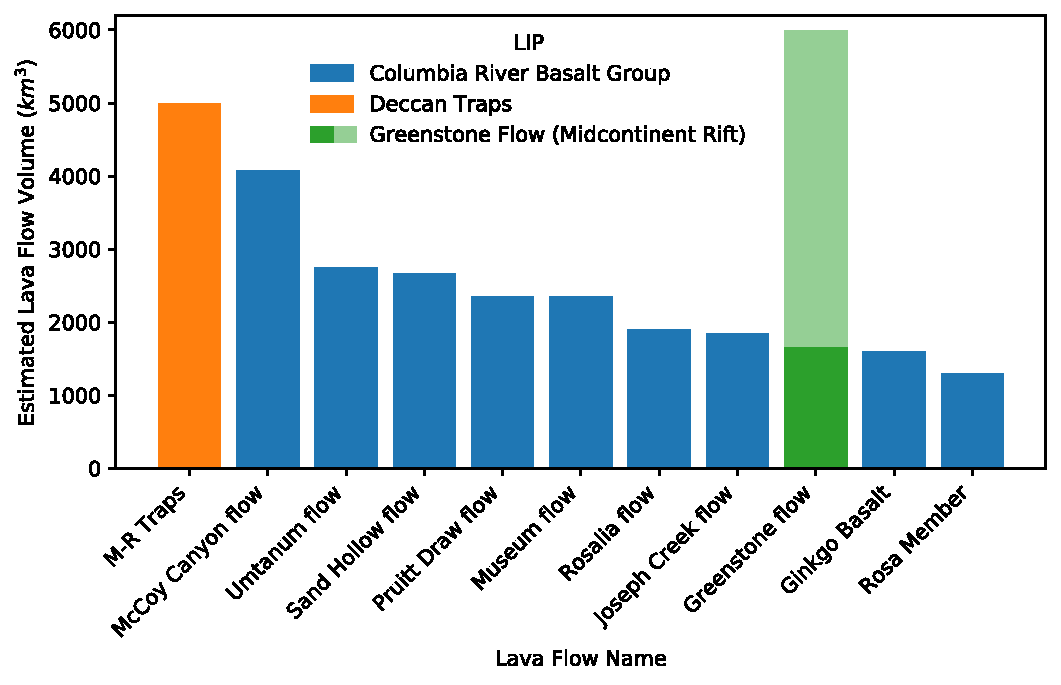
\includegraphics[width=\textwidth]{figure/Zhang2021/Lava_flow_rank.pdf}
\caption[Bar plot of ten of the world's most voluminous single mafic lava flows currently known.]{\footnotesize{Bar plot of ten of the world's most voluminous single mafic lava flows currently known. With an estimated minimum volume of $\sim$1650 km$^3$ and likely volume as high as $\sim$6000 km$^3$, the Greenstone Flow from the 1.1 Ga Midcontinent Rift stands amongst the giant lava flows from the Deccan Traps and Columbia River basalts. M-R Traps = Mahabaleshwar--Rajahmundry lava flow in the Deccan Traps. Volume estimates from \cite{Self2008a}, \cite{Bryan2010a}, \cite{Longo1984a}, and \cite{Doyle2016a}.}}
\label{fig:lava_flow_rank}
\end{figure}

One distinctive feature of the Beaver River diabase is its inclusions of anorthosite xenoliths. In the southern part of the Beaver Bay Complex, the Beaver River diabase occurs as dikes and sills, typically including anorthosites with various sizes ranging from centimeters to over 150 meters (Figs. \ref{Chap_BBC_Geologic_map}, \ref{fig:Chap_BBC_Field_photo}; \citealp{Grout1939a, Morrison1983a}). The diabase in this region intrudes the Palisade rhyolite of the North Shore Volcanic Group (Fig. \ref{Chap_BBC_Geologic_map}), which has a $^{206}$Pb/$^{238}$U date of 1093.94 $\pm$ 0.28 Ma (2$\sigma$ analytical uncertainty is presented for CA-ID-TIMS dates throughout this work; \cite{Swanson-Hysell2019a}). The Beaver River diabase is locally intruded by the Silver Bay intrusions (Fig. \ref{Chap_BBC_Geologic_map}). An aplite unit within the granophyre zone of one of these Silver Bay intrusions has a $^{206}$Pb/$^{238}$U date of 1091.61 $\pm$ 0.14 Ma \citep{Swanson-Hysell2019a}. Another arcuate, sill-like diabase body mapped as the Beaver River diabase outcrops along the eastern part of the complex (Fig. \ref{Chap_BBC_Geologic_map}; \citealp{Miller1997a}). The diabase composition there is similar to that in the south and it also contains large anorthosite xenoliths with dimensions that exceed 100 meters at Carlton Peak (Fig. \ref{Chap_BBC_Geologic_map}). The Beaver River diabase in the northern part of the complex, near the Houghtaling Creek area, typically forms narrow, near-vertical dikes instead of sheets in the southern and eastern regions (Fig. \ref{Chap_BBC_Geologic_map}; \citealp{Miller1994a}). The diabase in this region only locally contains xenoliths of anorthosite. 

Hundreds of anorthosite xenoliths have been recognized and mapped within the Beaver River diabase (Fig. \ref{Chap_BBC_Geologic_map}). Many hill tops in the Beaver Bay Complex, such as Carlton Peak and Britton Peak, are large anorthosite blocks (which lead \cite{Lawson1893a} to erroneously conclude that they were relict Archean topography). Later work established the anorthosite blocks as xenoliths, which are now extensively documented through geologic mapping of the region (Fig. \ref{Chap_BBC_Geologic_map}; \citealp{Miller2001a, Miller1988a, Miller1989a, Boerboom2004a, Boerboom2006a, Boerboom2006b, Boerboom2007a}) and outcrop-scale exposures (Fig. \ref{fig:Chap_BBC_Field_photo}). In the field, the anorthosites typically appear as subrounded to rounded, light-colored, translucent blocks that are in sharp contact with the hosting diabase (Fig. \ref{fig:Chap_BBC_Field_photo}). They also occur as exposures whose contact with the diabase is covered (Fig. \ref{fig:Chap_BBC_Field_photo}). \cite{Grout1939a} suggested that the rounded anorthosites are the result of abrasion during transportation as they were entrained by the diabase (i.e. physical weathering within a magmatic system). While the Beaver River diabase is chilled against the North Shore Volcanic Group lithologies that it intrudes, the diabase is not chilled against the margin of the anorthosite xenoliths \citep{Morrison1983a, Miller1997a}. The lack of chilled contacts is consistent with the anorthosite being at elevated temperatures and cooling at the same time as the diabase magma (Fig. \ref{fig:thermal_history_model}).

The anorthosite xenoliths are dominantly monomineralic plagioclase that has an average anorthite content of $\sim$70\% \citep{Morrison1983a, Doyle2016a}. Interstitial pyroxene and olivine are present in minor concentrations in the xenoliths. Within the Carlton Peak anorthosite xenolith, up to 10 cm oikocrysts of olivine and pyroxene can occur. Nevertheless, the overall olivine content in the anorthosites is low. Interstitial titanomagnetite-ilmenite intergrowths that exceed 100 $\mu$m can be found with microscopy and $<$20 $\mu$m Fe-Ti oxide grains can be detected with scanning electron microscopy (Fig. \ref{fig:Chap_BBC_Field_photo}). Based on textural differences \cite{Morrison1983a} divided the anorthosite xenoliths into four groups: one group which typically have well-developed granoblastic texture characterized by equigranular plagioclase crystals; another group which have interlocking, lath-shaped plagioclase crystals; an intermediate group which can have both granoblastic texture and interlocking plagioclase laths; and a brecciated group that have brittle deformation textures superposed on pre-existing textures. 

\subsection{Portage Lake Volcanics and the Greenstone Flow}

The Portage Lake Volcanics (PLV) is a $\sim$5 km thick, normally magnetized, dominantly olivine basalt to andesite volcanic succession that outcrops in northern Michigan (particularly along the Keweenaw Peninsula) as well as on Isle Royale (Fig. \ref{Chap_BBC_Geologic_map}; \citealp{Huber1973a, Cannon2001a, Green1982a}). The Greenstone Flow of the Portage Lake Volcanic Group has been recognized as one of the largest lava flows on earth (Figs. \ref{Chap_BBC_Geologic_map}, \ref{fig:lava_flow_rank}). It outcrops as the main ridge along the Keweenaw Peninsula and Isle Royale (Fig. \ref{Chap_BBC_Geologic_map}). The flow can be correlated between the two outcrop regions on the basis of geochemical, petrographic, and paleomagnetic similarity of the flow itself and the flows above and below \citep{Longo1984a}. In both outcrop regions, the Greenstone Flow is underlain by conglomerate and overlain by pyroclastic breccia \citep{Lane1911a, Huber1973a}. On the Keweenaw Peninsula, the Greenstone Flow is exposed over 90 km with a range of thickness from $\sim$100 meters to a maximum thickness of over 450 meters, dipping to the northwest (Fig. \ref{Chap_BBC_Geologic_map}; \citealp{White1960a}). On Isle Royale, the Greenstone Flow has a range of thickness from $\sim$30 meters to a maximum thickness of about 250 meters, dipping toward the southeast (Fig. \ref{Chap_BBC_Geologic_map}; \citealp{Huber1973a}). More recently, \cite{Doyle2016a} estimated that the total aerial extent of the Greenstone Flow could be up to $\sim$20000 km$^2$ by connecting it to the region of the Beaver Bay Complex. Taking thickness range of 100 to 300 meters, \cite{Doyle2016a} estimated a total volume of 2000 to 6000 km$^3$. This volume range makes the Greenstone Flow one of the largest, if not the largest, single mafic lava flows on Earth (Fig. \ref{fig:lava_flow_rank}).

According to the mineralogical and textural attributes, the Greenstone Flow can be divided into four zones from bottom to top --- a lower ophitic zone, a ``pegmatoid'' or heterolithic zone, an upper ophitic zone, and an amygdaloidal zone \citep{Cornwall1951b}. The heterolithic zone contains lenses to layers of coarse-grained granophyric gabbro that are referred to in the literature as ``pegmatoid.'' Zircon crystallized in these layers have enabled the heterolithic zone to be targeted for U-Pb geochronology \citep{Davis1990a, Swanson-Hysell2019a}. A $^{206}$Pb/$^{238}$U zircon date of 1091.59 $\pm$ 0.27 Ma for the Greenstone Flow was developed from a sample from this zone in \cite{Swanson-Hysell2019a}. The Greenstone Flow is typically interpreted to represent emplacement of a single body of magma that then underwent in situ differentiation \citep{Huber1973a, Davis1990a}. \cite{Doyle2016a} favored a distinct model in which the Greenstone Flow is a composite unit, which they interpret to be indicated by lithologic zonation of ophitic basalt forming the upper and lower zones and an interior zone composed of prismatic ferrogabbro to granophyric monzodiorite. They envision emplacement of the Greenstone Flow started with voluminous eruption of olivine tholeiitic magma, forming the ophitic zones which, while still crystallizing, further inflated due to subsequent injection of a more evolved basaltic magma to form intergranular gabbro in the heterolithic zone. They considered this progression to be more consistent with observed abrupt lithologic changes from the ophitic zone to the heterolithic zone over centimeter to meter scales, inclusion relationships between evolved and ophitic Greenstone Flow lithologies, and remnant blocks of initially crystallized ophitic basalt interlayered with evolved lithologies within the heterolithic zone which contains the pegmatoids. In both the \cite{Doyle2016a} model of multiple magma injections and the earlier models of in situ differentiation, it is the migration of the most evolved and volatile-rich melts within the interior of the flow in the final stages of flow crystallization that led to the formation of some aplite dikes and the coarsest segregations containing granophyre. Both models also invoke a single basaltic parental magma with distinction of where differentiation occurred in fractionally crystallizing an evolving magma chamber or solely within a single, very thick flow.

\section{Methods and Results}

\subsection{Zircon Geochronology and Geochemistry}

A sample of an anorthosite xenolith within the Beaver River diabase was collected for U-Pb geochronology along Hwy 61 across from the Silver Bay taconite plant (MS99033; 91.26358\textdegree W 47.28888\textdegree N; Fig. \ref{Chap_BBC_Geologic_map}). This sample comes from the same xenolith sampled for paleomagnetic study as site AX16 which has an exposed diameter of 27.5 meters (Fig. \ref{fig:Chap_BBC_Field_photo}). Thin sections were made from the geochronology sample as well as multiple paleomagnetic cores. As is shown in Fig. \ref{fig:Chap_BBC_Field_photo}F, plagioclase in this anorthosite xenolith have both equigranular crystals displaying a granoblastic texture and lath-shaped crystals displaying an interlocking texture. The occurrence of both textures is consistent with an interpretation that this anorthosite xenolith formed under elevated temperatures and experienced heating after initial crystallization. 

Zircons were separated from a kilogram of the anorthosite using common mineral separation methods (Supporting Information). The separated zircons were subhedral to anhedral crystals (z1-z4) and platy fragments (z5-z8). The subhedral to anhedral crystals are consistent with intercumulus crystallization within an adcumulate with platy fragments also being a common zircon morphology within anorthosites (e.g. sample AS3 of the Duluth Complex anorthositic series; \cite{Schmitz2003a}). Eight chemically abraded zircons were analyzed by isotope dilution-thermal ionization mass spectrometry (ID-TIMS) in the Boise State Isotope Geology Laboratory using EARTHTIME tracer solutions \citep{Condon2015a}. Both zircon morphologies yield indistinguishable dates. Using six of these single grain dates (and excluding two due to interpreted Pb-loss) results in a weighted mean $^{206}$Pb/$^{238}$U date of 1091.83 $\pm$ 0.21/0.37/1.15 Ma (analytical/ analytical+tracer/ analytical+tracer+decay uncertainty; Fig. \ref{fig:BBC_geochron}). 

\begin{figure}
\noindent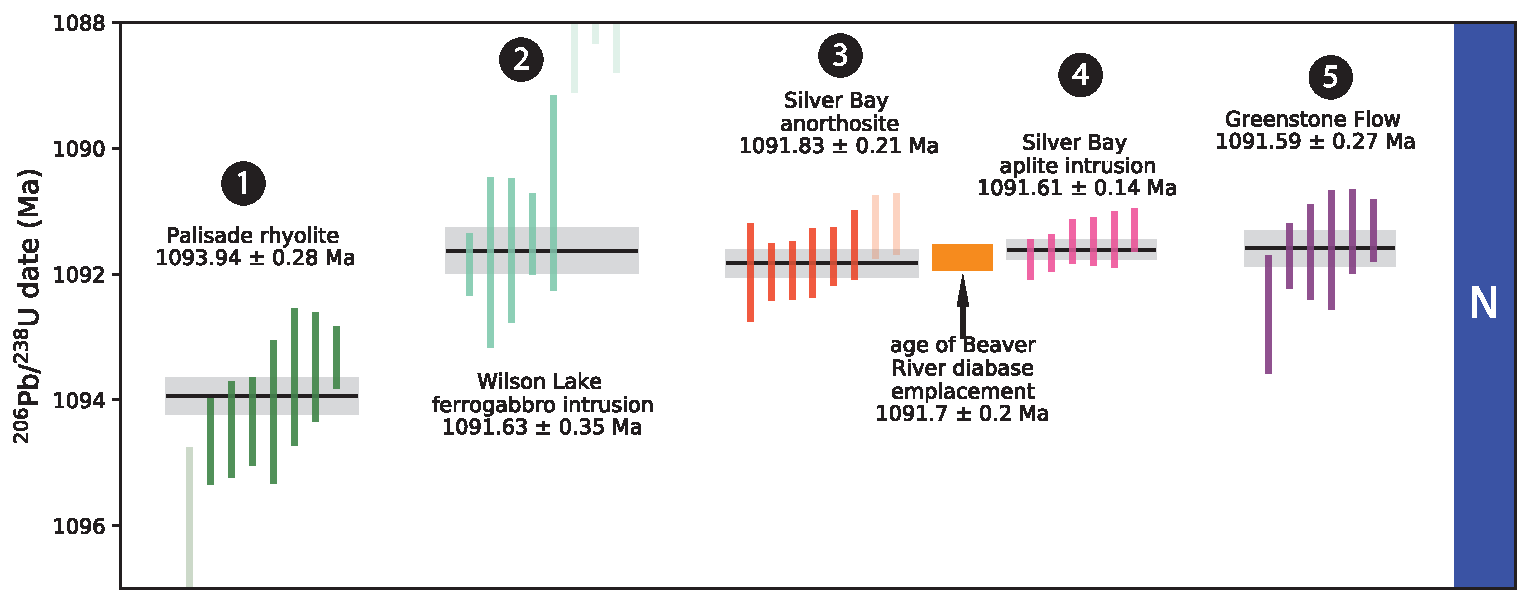
\includegraphics[width=\textwidth]{figure/Zhang2021/BBC_dates.pdf}
\caption[$^{206}$Pb/$^{238}$U zircon ages]{\footnotesize{New $^{206}$Pb/$^{238}$U zircon date of the anorthosite xenolith (dark orange) plotted in context of previously published $^{206}$Pb/$^{238}$U zircon dates from the North Shore Volcanic Group (NSVG) and other Beaver Bay Complex intrusions \citep{Swanson-Hysell2019a, Swanson-Hysell2021a}. These high-precision dates are consistent with field observations that the Beaver River diabase crosscuts the Palisade rhyolite (dark green) and is cut by the Silver Bay intrusions (pink). The estimated age of the Beaver River diabase from these constraints is shown by an orange box representing the 95$\%$ confidence interval. Each vertical bar corresponds to one $^{206}$Pb/$^{238}$U date from a single zircon crystal. The translucent bars represents zircons with interpreted Pb loss and are therefore not included in the weighted mean age calculations. Horizontal lines and gray boxes represent weighted mean $^{206}$Pb/$^{238}$U dates and their analytical uncertainty. The numbers of each geochronology sample correspond to those in Fig. \ref{Chap_BBC_Geologic_map} where locations of these samples are shown.}}
\label{fig:BBC_geochron}
\end{figure}

This date provides a tight constraint on the age of the Beaver River diabase. Previously, the maximum age constraint for the Beaver River diabase came from the relationship that it cross-cuts the Palisade rhyolite of the North Shore Volcanic Group which has a $^{206}$Pb/$^{238}$U date of 1093.94 $\pm$ 0.28 Ma  \citep{Swanson-Hysell2019a}. With this new date, we know the crystallization age of the diabase to have been near-synchronous or younger than the date from the anorthosite xenolith. The Silver Bay intrusions, from which an aplite has a $^{206}$Pb/$^{238}$U date of 1091.61 $\pm$ 0.14 Ma, \citep{Fairchild2017a}, cross-cut the Beaver River diabase. These dates constrain the diabase to have been emplaced between 1091.83 $\pm$ 0.21 and 1091.61 $\pm$ 0.14 Ma (Fig. \ref{fig:BBC_geochron}). Assuming a uniform probability of diabase emplacement between the anorthosite and aplite dates and their normal distributed uncertainties, a 95\% confidence interval on the age of the diabase can be estimated by Monte Carlo simulation. This analysis gives an age for the diabase of 1091.7 $\pm$ 0.2 Ma (95\% CI). 

\begin{figure}[h!]
\noindent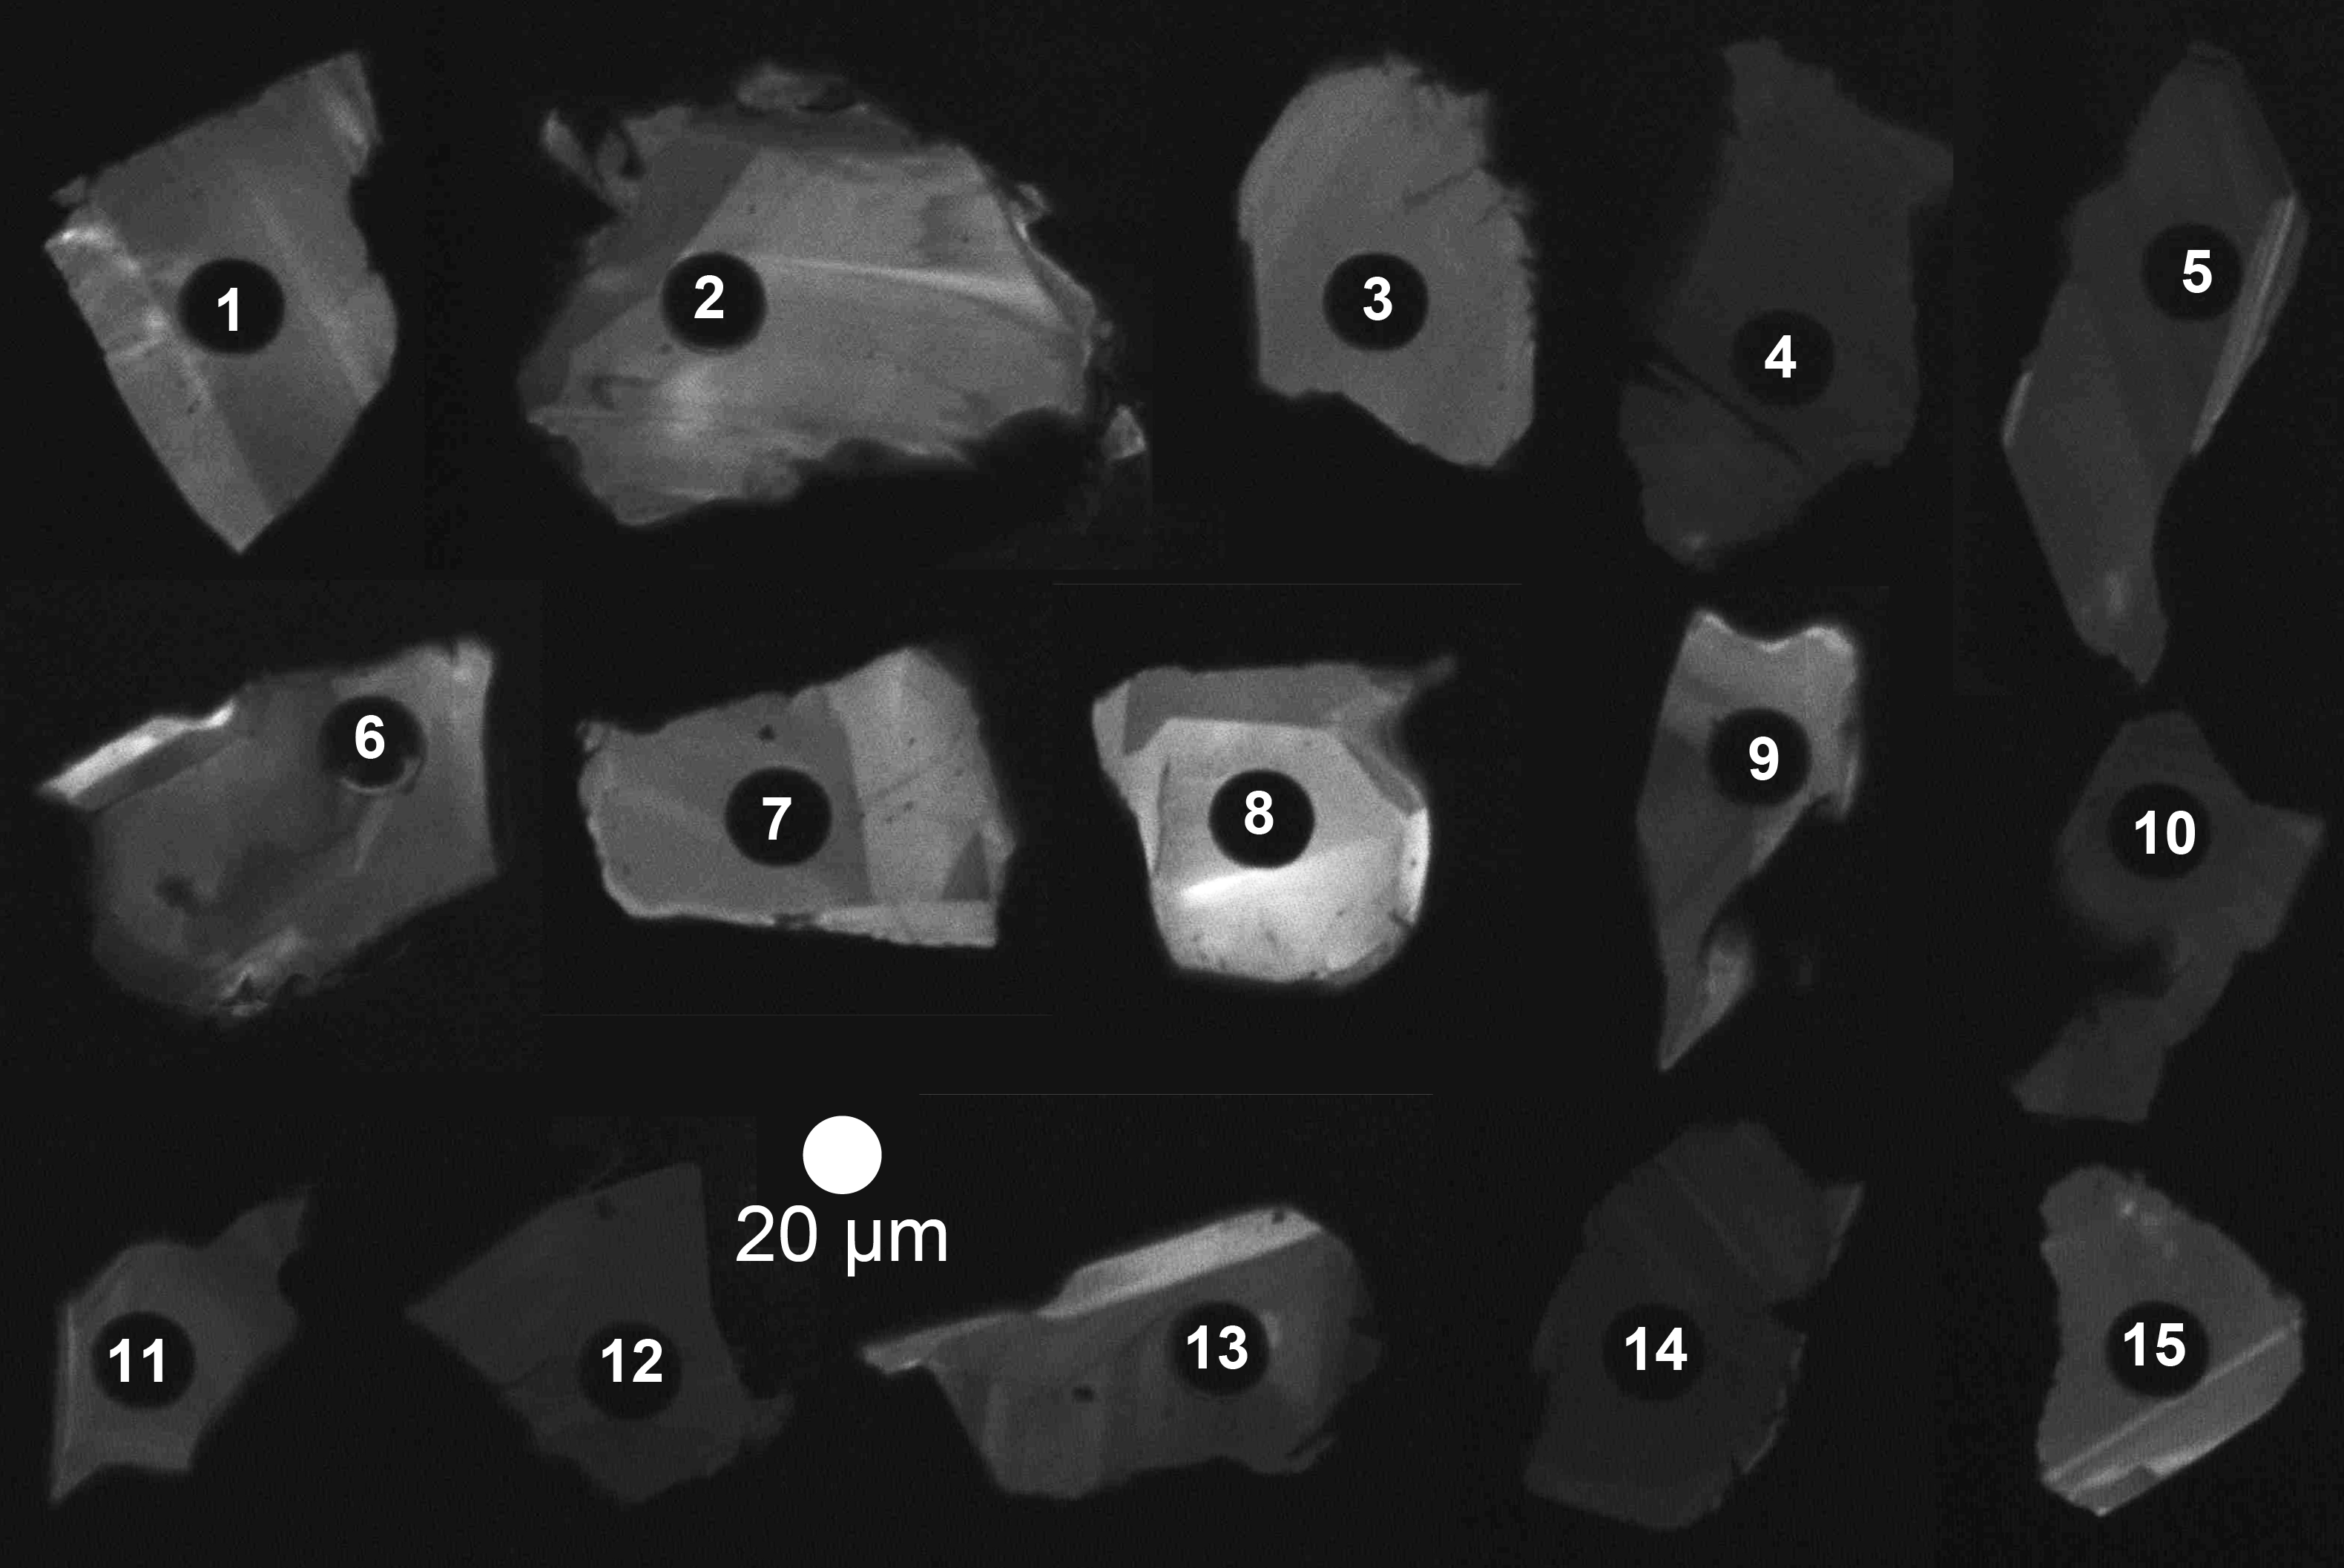
\includegraphics[width=\textwidth]{figure/Zhang2021/CL_montage.png}
\centering
\caption[Cathodoluminescnece (CL) image montage of the 15 zircons laser-ablated for trace element analysis from sample MS99033.]{\footnotesize{Cathodoluminescnece (CL) image montage of the 15 zircons laser-ablated for trace element analysis from sample MS99033. There are sharp boundaries between zones of differing CL response within many of the zircons attributable to variable REE concentrations. For example, the bright zoning in grain 15 has a thickness of $\sim$2 $\mu$m. Note that grain 1 (corresponding to spot 1) has a platy morphology, while the rest of the grains are subhedral to anhedral.}}
\label{fig:CL_image}
\end{figure}

\begin{figure}[h!]
\noindent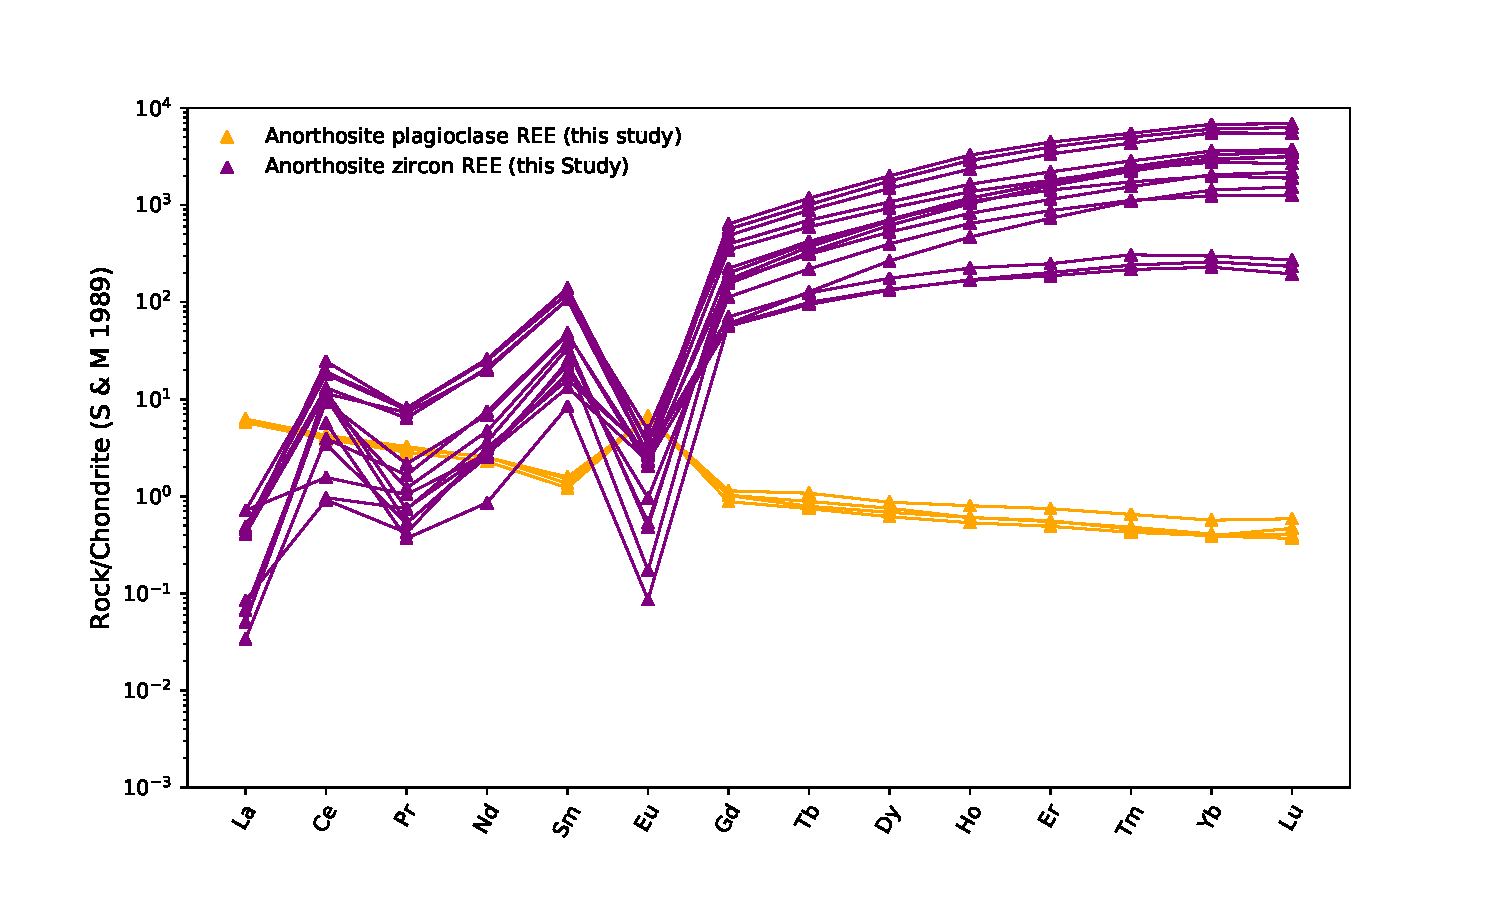
\includegraphics[width=\textwidth]{figure/Zhang2021/REE.pdf}
\centering
\caption[Rare earth element (REE) analyses for plagioclase crystals from anorthosite xenoliths and for 15 zircons from geochronology sample MS99033]{\footnotesize{Rare earth element (REE) analyses for plagioclase crystals from anorthosite xenoliths and for 15 zircons from geochronology sample MS99033 (anorthosite xenolith site AX16) developed by inductively coupled plasma mass spectrometry. All data are chrondrite-normalized \citep{Sun1989a}.}}
\label{fig:REE}
\end{figure}

An additional 15 zircons were characterized using cathodoluminescence (CL) imaging and laser ablation-inductively coupled plasma mass spectrometry (LA-ICPMS), with methods and instrumentation described in the Supporting Information. CL images reveal internal planar zones of variable brightness, often with darker interior zones and brighter outer zones (Fig. \ref{fig:CL_image}). All crystals exhibit sharp, micron-scale transitions between zones, and LA-ICPMS analyses quantify CL brightness as correlated with rare earth elements (REE) content. REE patterns in zircons exhibit a significant chondrite-normalized negative Eu anomaly (Fig. \ref{fig:REE}). The Ti-in-zircon thermometer gives a range of estimated zircon crystallization temperatures from 998\textdegree C to 860\textdegree C with a mean of $\sim$950\textdegree C (\citealp{Ferry2007a}; Supporting Information). Decreasing temperatures are correlated with deepening of the negative Eu anomaly and increasing incompatible trace element (e.g. Hf, Th) incorporation into zircon. These data are consistent with a model of magmatic zircon crystallizing from cooling and fractionating interstitial residual melt within the cumulate plagioclase framework.

\subsection{Paleomagnetism}

We collected paleomagnetic cores that are 2.5 cm in diameter along the southern and eastern Beaver Bay Complex with a particular focus on acquiring paired sites of anorthosite xenoliths and their local diabase hosts. Sample cores were collected using a hand-held gasoline-powered drill and were oriented using a magnetic compass as well as a sun compass when possible. Sun compass orientations were preferentially used for determining the sample azimuth. Typically, 7-10 cores were collected for each anorthosite xenolith and their diabase hosts. A total of 17 diabase and 22 anorthosite sites were sampled (Table \ref{tab:Pmag_site_data}). A table that summarizes the measured dimensions of each anorthosite xenolith sampled and the distance between each anorthosite paleomagnetic site and closest diabase host site is provided in the Supporting Information.  

Samples underwent step-wise demagnetization and analyses in the magnetically-shielded room at the UC Berkeley Paleomagnetism Lab. 7 sites from the Beaver River diabase underwent alternating field (AF) demagnetization with peak fields from 1 mT to 130 mT. An ASC TD-48SC thermal demagnetizer was used to demagnetize 10 diabase sites and all 22 anorthosite sites in a step-wise manner, with reduced step increments between 540\textdegree C and 585\textdegree C. The typical magnetic field inside the shielded room is $<$500 nT and the field inside the thermal demagnetizer chamber is $<$10 nT. The quartz glass sample rod of the UC Berkeley system is typically measured at 5 $\times$ 10$^{-12}$ Am$^{2}$. All remanence measurements were made on a 2G Enterprises DC-SQUID superconducting rock magnetometer equipped with inline AF coils and an automated sample changer system. The PmagPy software package was used to implement least-square fits to specimen demagnetization data \citep{Tauxe2016a}. Measurement level data are available within the MagIC database (\url{https://earthref.org/MagIC/doi/10.1029/2021GC009909})

\begin{figure}
\centering 
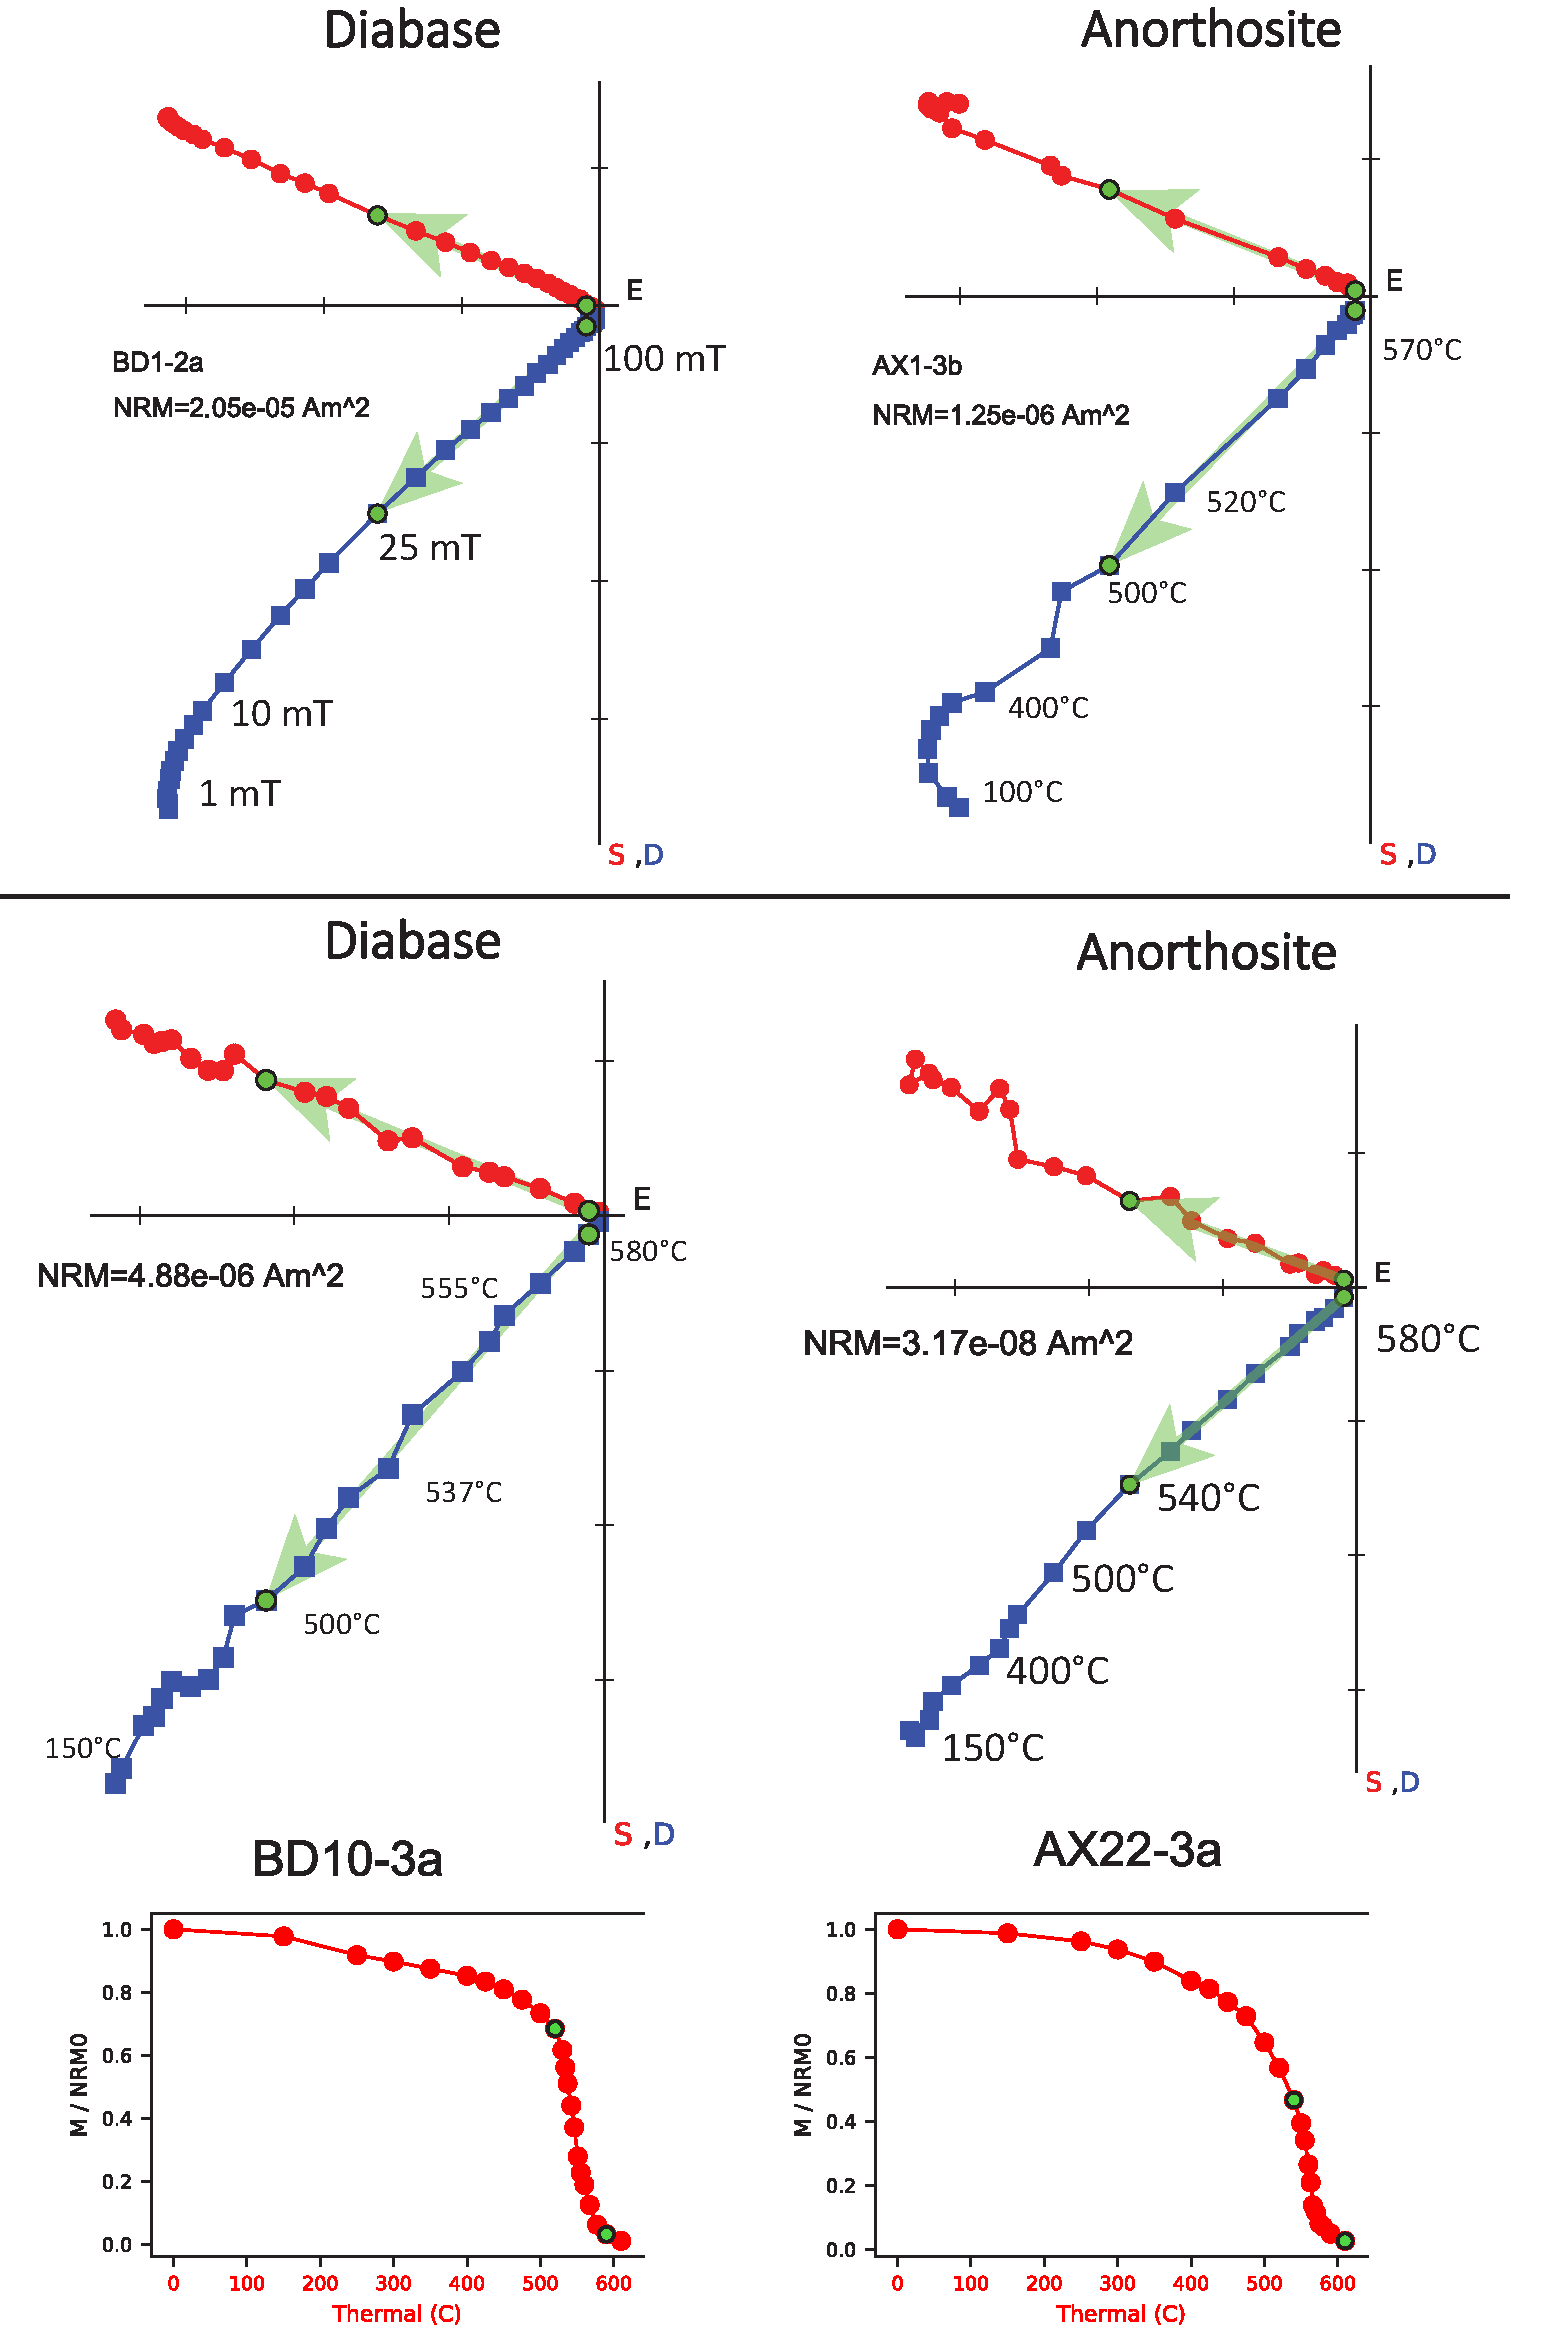
\includegraphics[width=0.65\textwidth]{figure/Zhang2021/Demag.pdf}
\caption[Example orthogonal vector demagnetization diagrams for diabase and anorthosite specimens]{\small{Example orthogonal vector demagnetization diagrams for diabase and anorthosite specimens. Anorthosite site AX1 is a xenolith within the diabase sampled as BD1. Similarly, AX22 is from a xenolith within the BD10 diabase. Both AF and thermal demagnetization show dominantly univectoral decay of characteristic remanent magnetizations (ChRM) toward the origin after removal of minimal secondary components. The data show very similar ChRM directions between the paired diabase and anorthosite xenoliths sites. Representative magnetization intensity versus thermal demagnetization step plots are paired with orthogonal vector plots for specimen BD10-3a and AX22-3a.}}
\label{fig:Demag}
\end{figure}

For both the diabase and anorthosite demagnetization, principal component analyses show that an origin trending characteristic remanent magnetization (ChRM) can be isolated after the removal of a minimal secondary component during the first few low coercivity ($<$10 mT) or low temperature ($<$200\textdegree C) demagnetization steps (Fig. \ref{fig:Demag}). The ChRMs typically unblock through thermal demagnetization steps from $\sim$500\textdegree C to $\sim$580\textdegree C, consistent with the component being held by low-titanium titanomagnetite. We interpret this component as a primary remanent magnetization acquired during the emplacement and cooling of the Beaver River diabase.

The site mean paleomagnetic directions are shown in Table \ref{tab:Pmag_site_data}. We present both AF and thermal demagnetization results for the Beaver River diabase as both methods are effective in removing the secondary components and isolating the coherent and univectoral ChRM. Based on specimen and site level demagnetization behavior and the proximity between paired paleomagnetic sites of the anorthosite xenoliths and the diabase, we grouped the anorthosite xenoliths and their diabase hosts into individual cooling units and calculated a paleomagnetic pole position from the mean of the cooling unit virtual geomagnetic poles (Fig. \ref{fig:Direction_pairs}). 

\begin{figure}
\noindent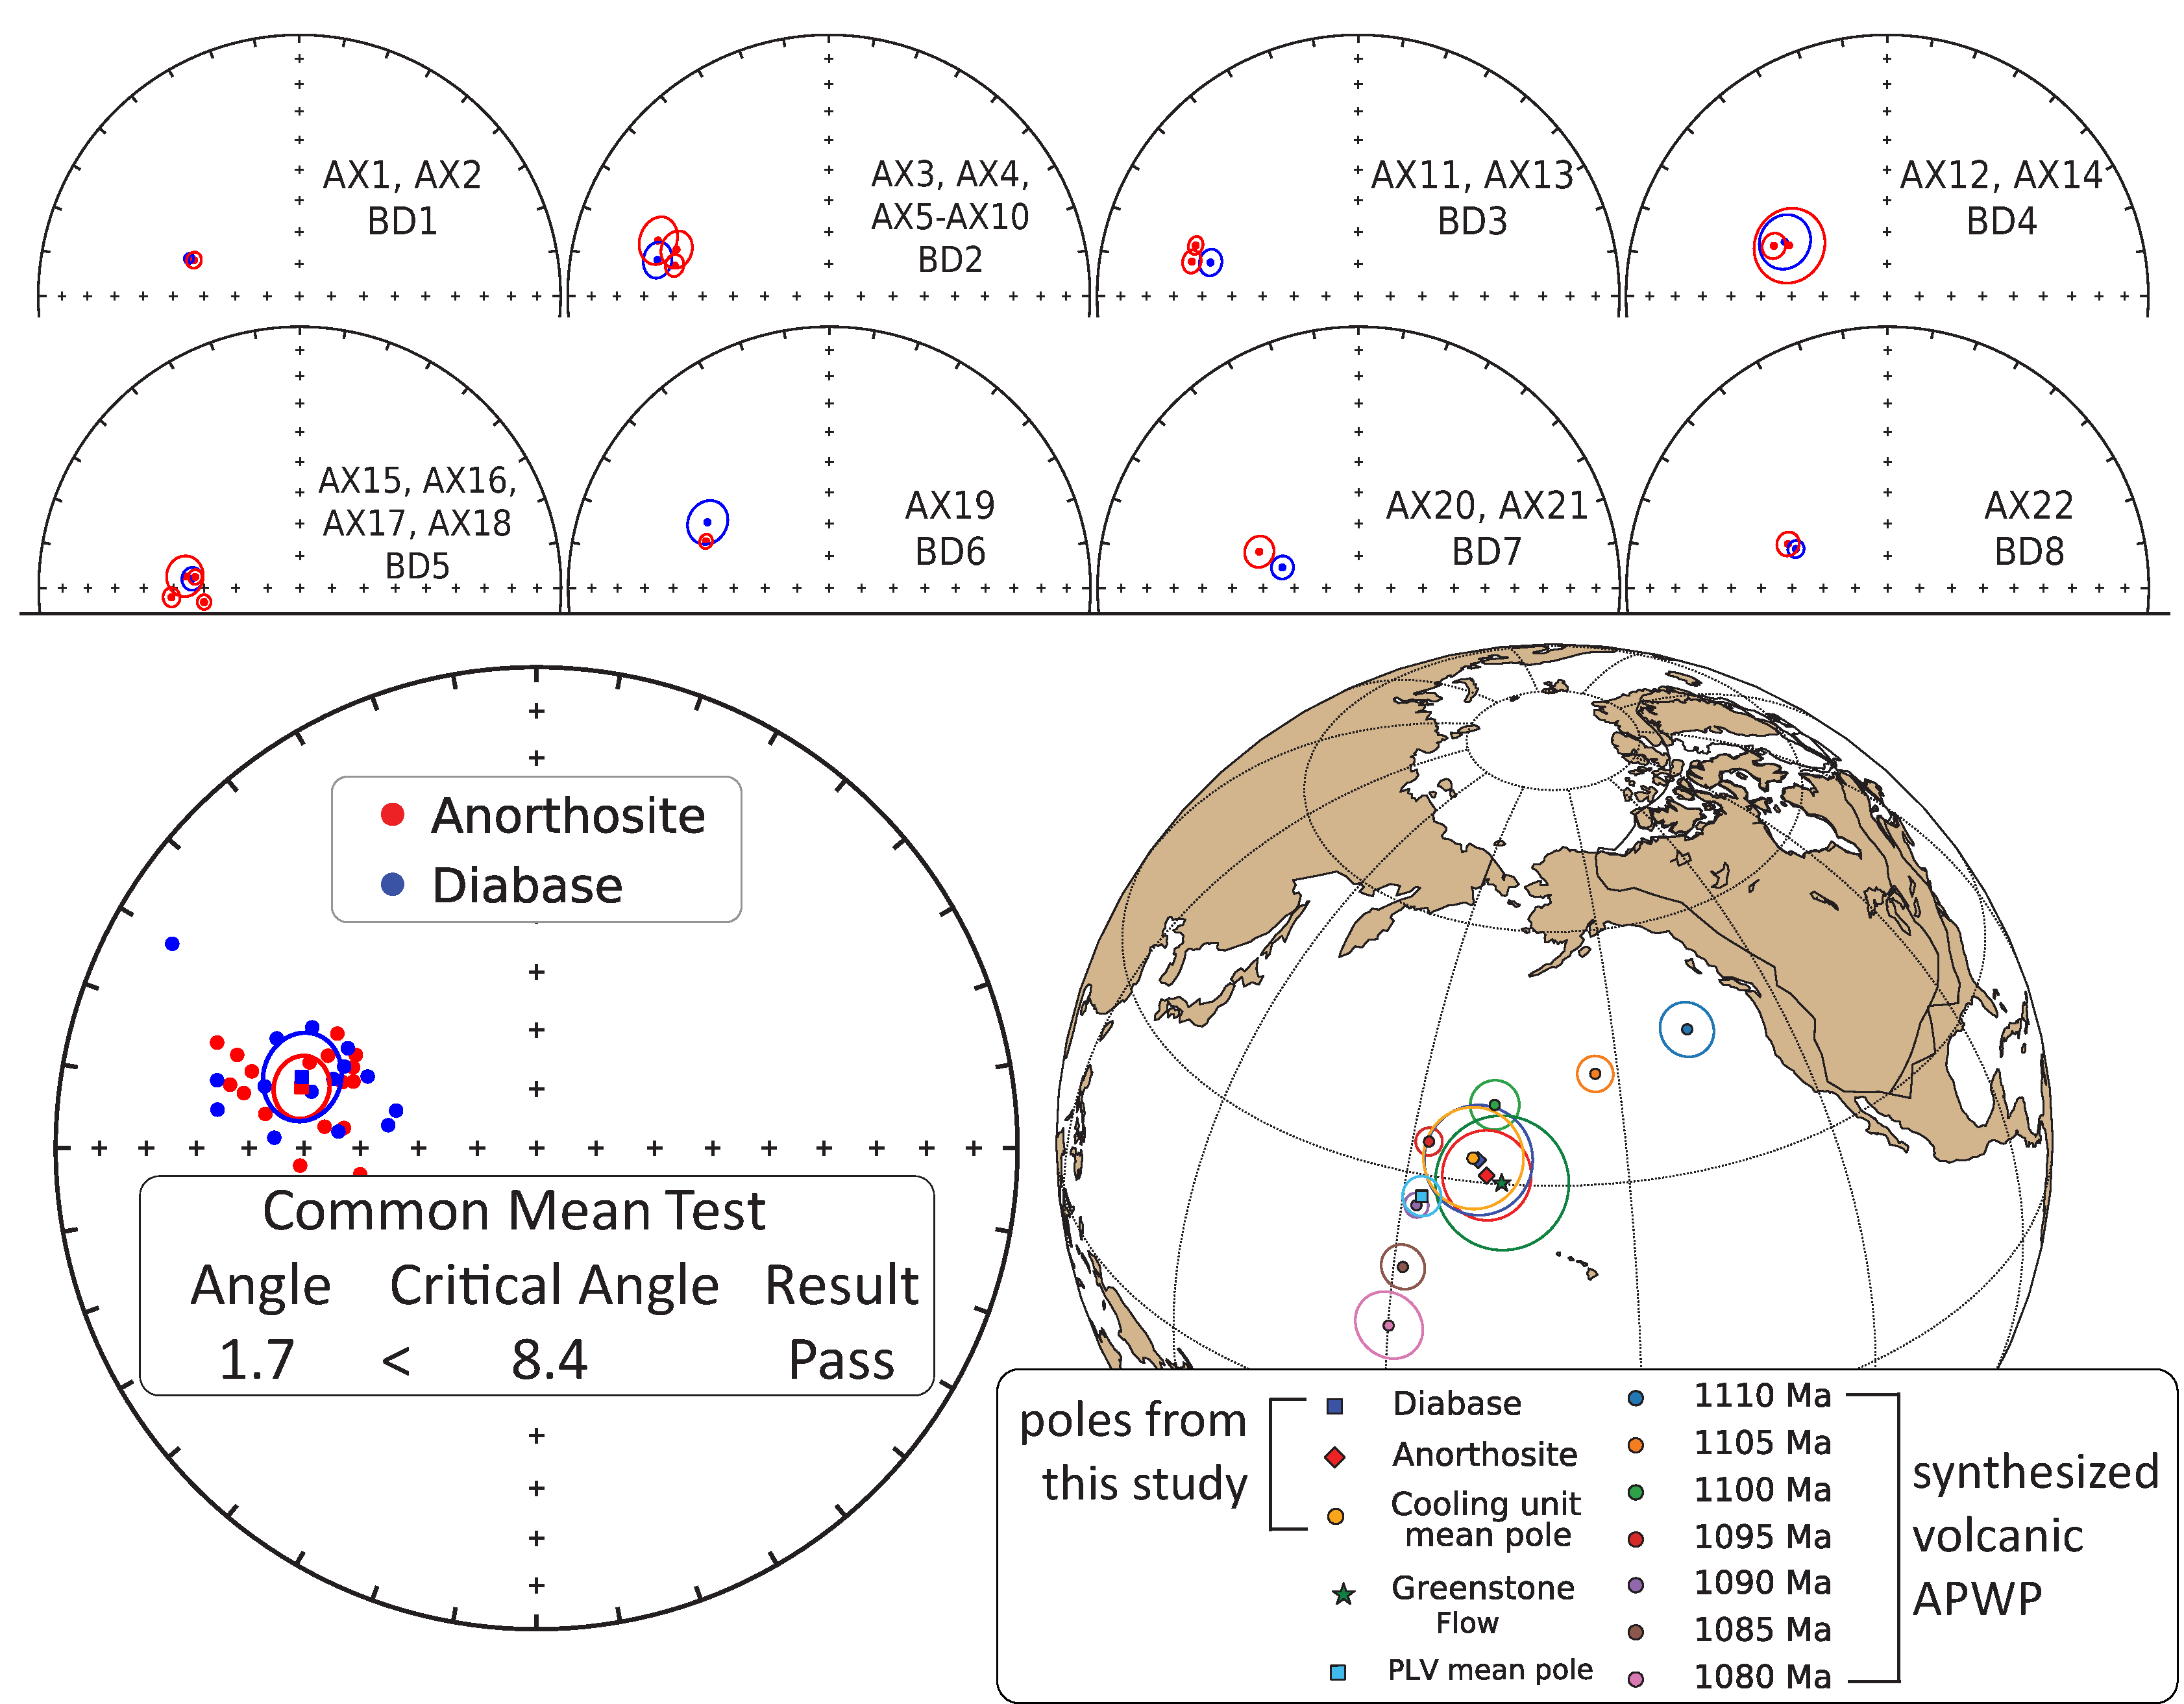
\includegraphics[width=\textwidth]{figure/Zhang2021/Direction_pairs.pdf}
\caption[Summary equal area plots and paleomagnetic pole plots]{\small{Top: Equal area plots of paleomagnetic directions from the anorthosite xenoliths and their local diabase hosts. AX: anorthosite xenolith site; BD: Beaver River diabase site. Bottom: Site mean paleomagnetic directions from the Beaver River diabase and anorthosite xenoliths are plotted on equal area plots. The anorthosite and diabase sites share a common mean as summarized by the results of the \cite{McFadden1990a} common mean test. Mean paleomagnetic pole positions of all diabase sites, all anorthosite sites, as well as a grand mean pole developed by grouping the anorthosite and diabase sites into individual cooling units are plotted against a synthesized Laurentia APWP based on poles from Midcontinent Rift volcanics and sedimentary rocks \citep{Swanson-Hysell2019a}. The paleomagnetic poles from the diabase and anorthosite are indistinguishable with the Greenstone Flow pole developed by \cite{Foucher2018a}, but they all are distinct from the Portage Lake Volcanics mean pole \citep{Swanson-Hysell2019a}. All directions shown are tilt corrected.}}
\label{fig:Direction_pairs}
\end{figure}

Tilt-correcting the paleomagnetic directions to paleohorizontal is necessary for developing accurate paleomagnetic poles from the diabase and the anorthosite xenoliths to be compared to the Keweenawan Track apparent polar wander path (APWP; Fig. \ref{fig:Direction_pairs}; \citealp{Swanson-Hysell2019a}). For intrusive igneous rocks, tilt corrections can be difficult to constrain due to the lack of a clear paleohorizontal reference. Many paleomagnetic studies of Midcontinent Rift intrusive rocks in the Lake Superior region did not apply tilt corrections to their data \cite[e.g.][]{Beck1969a, Beck1970a, Books1966a}. However, we can determine the structural orientation of the Beaver River diabase using the abundant igneous fabric orientations measured on the diabase as well as bedding orientations measured from adjacent volcanic units \citep{Boerboom2004a, Boerboom2006a, Boerboom2006b, Boerboom2007a, Miller2001a}. We compile the igneous layering measurements from the Beaver River diabase and the volcanic bedding orientations from the Schroeder-Lutsen basalt which is overlying the Beaver Bay Complex (Fig. \ref{Chap_BBC_Geologic_map}). Despite the uncertainties associated with using igneous fabrics orientations as paleohorizontal references, the mean tilt orientations of the fabrics of the Beaver River diabase and the volcanic bedding orientations of the Schroeder-Lutsen basalt are similar (diabase overall dip direction - dip: 128.5 - 10.2; basalt dip direction - dip: 142.2 - 13.6). We combine the structural measurements from the Beaver River diabase and the Schroeder-Lutsen basalt and derived two sets of tilt corrections for the paleomagnetic directions of the diabase and anorthosite (dip direction - dip in the southern Beaver Bay complex: 128.7 - 12.9; in the eastern Beaver Bay Complex: 145.6-13.1, Supporting Information). The advantage of using the structural orientations from the Schroeder-Lutsen basalt is that the arcuate shape of the Beaver River diabase intrusions is nicely captured by the variation of lava dip directions while the dip angles of the basalt and diabase are very similar (Fig. \ref{Chap_BBC_Geologic_map}).

The tilt-corrected ChRMs in both lithologies are west-northwest and down, yielding good specimen-level and site-level consistency (Figs. \ref{fig:Demag} and \ref{fig:Direction_pairs}). Close directional similarities between each anorthosite xenolith and their host diabase are supported by 9 out of a total of 17 diabase-anorthosite paleomagnetic site pairs passing a common mean test \citep{McFadden1990a}. The overall mean directions between the two lithologies are indistinguishable as they also pass a common mean test (Fig. \ref{fig:Direction_pairs}, \citealp{McFadden1990a}). For the anorthosite sites that do not pass a common mean test with their diabase hosts, they nevertheless have coherent specimen-level directions that are close to their host diabase directions (Fig. \ref{fig:Direction_pairs}). We also plot the tilt-corrected mean pole of sites from both lithologies (diabase: 32.5\textdegree N, 189.5\textdegree E, N = 15, A95 = 6.3, k = 37.4; anorthosite: 30.9\textdegree N, 190.8\textdegree E, N = 17, A95: 5.2, k = 48.5; Table. \ref{tab:Pmag_site_data}) in context of a previously synthesized APWP from the volcanics of the Midcontinent Rift \citep{Swanson-Hysell2019a} and show the poles to lie near the expected 1090 Ma and 1095 Ma pole positions (Fig. \ref{fig:Direction_pairs}). The mean pole position of the interpreted cooling units (32.7\textdegree N, 188.8\textdegree E, N = 15, A95 = 5.9, k = 41) lies close to the mean pole position derived from the ca. 1092 Ma Portage Lake Volcanics (Fig. \ref{fig:Direction_pairs}), consistent with the coeval magmatic activity between the Beaver River diabase and the Portage Lake Volcanics. If it is included in future Laurentia APWP compilations, it is this cooling unit mean pole paired with the estimated diabase emplacement age of 1091.7 $\pm$ 0.2 Ma that should be used.


\begin{sidewaystable}
\scriptsize
\caption[Summary of new site level paleomagnetic data for the Beaver River diabase and anorthosite xenoliths.]{\footnotesize Summary of new site level paleomagnetic data for the Beaver River diabase and anorthosite xenoliths. n/N: number of samples/sites analyzed and included in the site/grand mean; $dec_{is}$ \& $inc_{is}$: in situ mean declination and inclination for the site; $dec_{tc}$ \& $inc_{tc}$: tilt-corrected mean declination and inclination for the site; k: Fisher precision parameter; R: resultant vector length; $\alpha$95: 95\% confidence limit in degrees; VGP lat—latitude of the virtual geomagnetic pole for the site; VGP lon—longitude of the virtual geomagnetic pole for the site. Full measurement level data are available within the MagIC database. \url{https://earthref.org/MagIC/doi/10.1029/2021GC009909}.}
\centering
\begin{tabular}{cccccccccccccc}
\hline
site             & lat  & lon   & n/N  & $dec_{is}$ & $inc_{is}$ & $dec_{tc}$ & $inc_{tc}$ & k     & $\alpha_{95}$ & VGP $lat_{is}$ & VGP $lon_{is}$ & VGP $lat_{tc}$ & VGP $lon_{tc}$ \\
\hline
AX1              & 47.2 & -91.4 & 8.0  & 293.3   & 42.6         & 288.8   & 54.9    & 536.0 & 2.4                     & 33.4        & 180.0       & 37.1         & 193.2        \\
AX2              & 47.2 & -91.4 & 9.0  & 282.0   & 31.3         & 277.2   & 42.6    & 145.0 & 4.3                     & 20.4        & 181.8       & 22.6         & 191.1        \\
AX3              & 47.6 & -90.9 & 10.0 & 290.4   & 28.2         & 285.1   & 38.6    & 69.0  & 5.9                     & 24.7        & 174.5       & 25.9         & 183.7        \\
AX4              & 47.6 & -90.9 & 7.0  & 291.9   & 20.0         & 288.3   & 30.7    & 91.0  & 6.4                     & 22.3        & 169.8       & 24.4         & 177.2        \\
AX5-10           & 47.6 & -90.9 & 14.0 & 286.2   & 29.1         & 280.7   & 38.1    & 269.5 & 2.5                     & 22.3        & 178.1       & 22.7         & 186.5        \\
AX11             & 47.4 & -91.2 & 8.0  & 284.9   & 23.5         & 281.7   & 35.2    & 305.0 & 3.2                     & 19.1        & 176.3       & 22.0         & 184.1        \\
AX12             & 47.3 & -91.3 & 6.0  & 299.9   & 42.5         & 297.3   & 55.2    & 36.0  & 11.3                    & 37.8        & 175.1       & 43.0         & 188.4        \\
AX13             & 47.4 & -91.2 & 9.0  & 289.8   & 23.0         & 287.3   & 35.1    & 434.0 & 2.5                     & 22.2        & 172.4       & 25.7         & 180.0        \\
AX14             & 47.3 & -91.3 & 7.0  & 296.9   & 38.2         & 293.9   & 50.8    & 256.0 & 3.8                     & 33.7        & 174.5       & 38.2         & 186.1        \\
AX15             & 47.3 & -91.3 & 8.0  & 282.9   & 42.3         & 275.8   & 53.5    & 86.0  & 6.0                     & 26.2        & 187.2       & 27.9         & 199.8        \\
AX16             & 47.3 & -91.3 & 8.0  & 273.7   & 39.1         & 265.8   & 49.2    & 396.0 & 2.8                     & 18.5        & 191.6       & 19.0         & 202.9        \\
AX17             & 47.3 & -91.3 & 8.0  & 273.6   & 49.8         & 261.6   & 59.6    & 647.0 & 2.2                     & 24.3        & 198.3       & 23.7         & 213.5        \\
AX18             & 47.3 & -91.3 & 9.0  & 283.8   & 45.5         & 276.0   & 56.9    & 535.0 & 2.2                     & 28.5        & 188.7       & 30.2         & 202.8        \\
AX19             & 47.3 & -91.3 & 8.0  & 293.9   & 35.8         & 290.7   & 48.2    & 695.0 & 2.1                     & 30.5        & 175.4       & 34.6         & 186.0        \\
AX20             & 47.3 & -91.3 & 5.0  & 294.5   & 44.3         & 290.0   & 56.7    & 271.0 & 4.7                     & 35.1        & 180.4       & 39.0         & 194.5        \\
AX21             & 47.3 & -91.3 & 8.0  & 301.7   & 37.7         & 299.9   & 50.5    & 803.0 & 2.0                     & 36.7        & 170.4       & 42.1         & 181.7        \\
AX22             & 47.4 & -91.2 & 9.0  & 297.2   & 43.1         & 293.8   & 55.7    & 208.0 & 3.6                     & 36.3        & 177.6       & 41.0         & 191.1        \\
\hline
Anorthosite mean &      &       & 17.0 & 289.3   & 36.5         & 284.5   & 48.2    & 55.0  & 4.9                     & 28.0        & 179.6       & 30.9         & 190.8        \\
\hline
BD1              & 47.2 & -91.4 & 15.0 & 293.1   & 40.9         & 288.8   & 53.2    & 623.0 & 1.5                     & 32.4        & 179.0       & 36.1         & 191.6        \\
BD2              & 47.6 & -90.9 & 8.0  & 286.6   & 22.7         & 282.0   & 32.6    & 122.0 & 5.0                     & 19.9        & 175.0       & 21.0         & 182.8        \\
BD3              & 47.4 & -91.2 & 8.0  & 286.6   & 29.8         & 282.8   & 41.6    & 212.0 & 3.8                     & 22.9        & 177.9       & 25.8         & 186.9        \\
BD4              & 47.3 & -91.3 & 8.0  & 300.2   & 40.7         & 297.9   & 53.4    & 47.0  & 8.2                     & 37.1        & 173.6       & 42.3         & 186.0        \\
BD5              & 47.3 & -91.3 & 8.0  & 282.7   & 44.8         & 274.8   & 56.0    & 271.0 & 3.4                     & 27.4        & 188.9       & 28.9         & 202.6        \\
BD6              & 47.3 & -91.3 & 9.0  & 300.0   & 33.2         & 298.3   & 46.0    & 64.0  & 6.5                     & 33.4        & 169.2       & 38.6         & 178.9        \\
BD7              & 47.3 & -91.3 & 7.0  & 292.4   & 53.1         & 285.0   & 65.3    & 305.0 & 3.5                     & 38.5        & 189.2       & 41.3         & 208.3        \\
BD8              & 47.2 & -91.4 & 10.0 & 287.9   & 52.8         & 278.8   & 64.5    & 300.0 & 2.8                     & 35.3        & 191.8       & 37.1         & 209.9        \\
BD9              & 47.2 & -91.3 & 7.0  & 278.2   & 33.8         & 272.3   & 44.6    & 55.0  & 8.2                     & 19.0        & 185.7       & 20.4         & 195.6        \\
BD10             & 47.4 & -91.2 & 10.0 & 297.0   & 46.2         & 293.0   & 58.7    & 341.0 & 2.6                     & 37.8        & 180.0       & 42.2         & 195.1        \\
BD11             & 47.4 & -91.3 & 8.0  & 296.4   & 41.7         & 293.0   & 54.2    & 429.0 & 2.7                     & 35.1        & 177.1       & 39.5         & 189.9        \\
BD12             & 47.3 & -91.3 & 8.0  & 288.8   & 38.1         & 284.1   & 50.1    & 141.0 & 4.7                     & 28.1        & 180.4       & 31.3         & 191.8        \\
BD13             & 47.5 & -91.1 & 8.0  & 280.4   & 22.4         & 276.9   & 33.6    & 341.0 & 3.0                     & 15.6        & 179.2       & 18.0         & 186.7        \\
BD15             & 47.7 & -90.6 & 8.0  & 300.1   & 2.3          & 299.3   & 14.2    & 119.0 & 5.1                     & 20.6        & 156.9       & 24.8         & 161.7        \\
BD17             & 47.4 & -91.2 & 8.0  & 295.1   & 28.5         & 292.9   & 41.0    & 550.0 & 2.4                     & 28.0        & 170.8       & 32.3         & 179.3        \\
\hline
Diabase mean     &      &       & 15.0 & 291.0   & 35.7         & 286.9   & 47.7    & 51.6  & 5.0                     & 29.0        & 178.2       & 32.5         & 189.5       \\
\hline
\end{tabular}
\label{tab:Pmag_site_data}
\end{sidewaystable}


\subsection{Thermal history model}

\begin{figure}
\noindent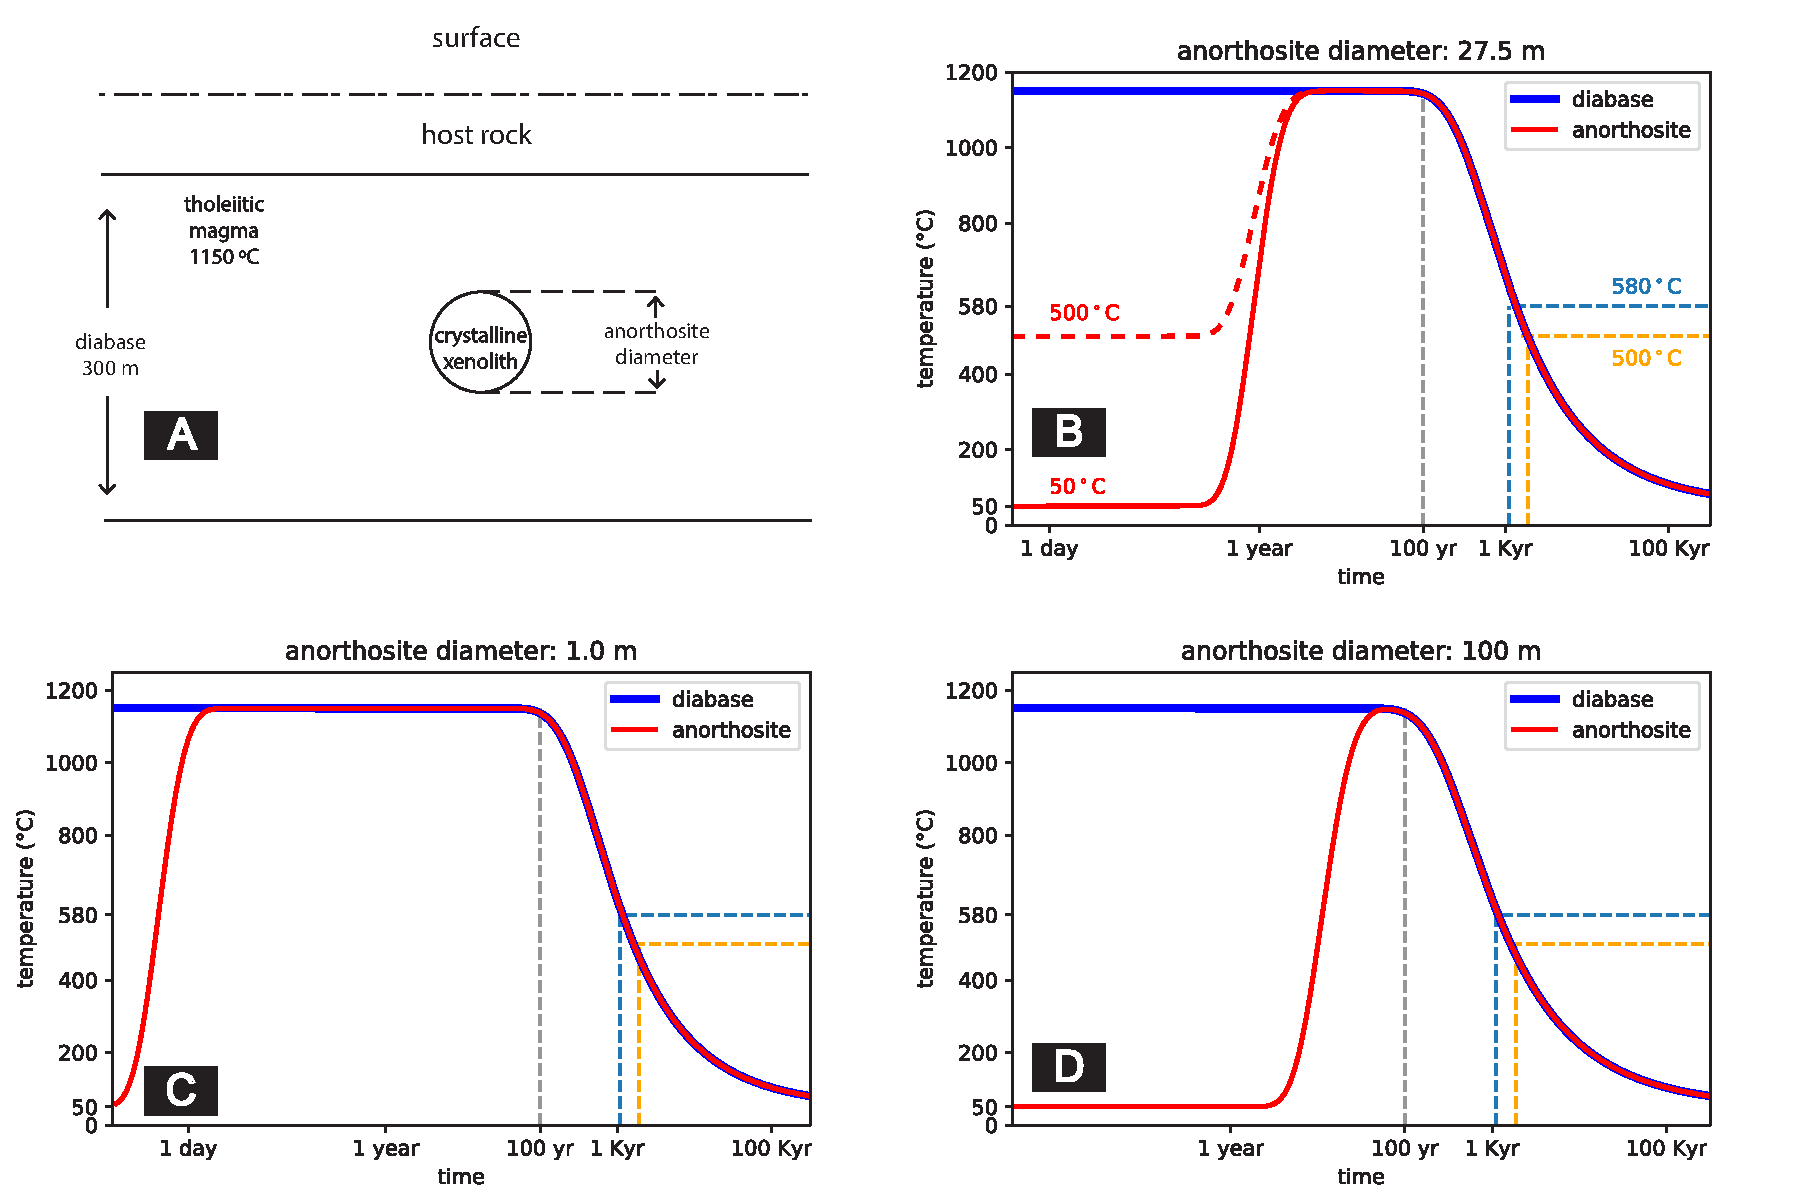
\includegraphics[width=\textwidth]{figure/Zhang2021/thermal_history_model.pdf}
\caption[Thermal history model of the Beaver River diabase and its anorthosite xenoliths after emplacement at hypabyssal depths.]{\footnotesize{Thermal history model of the Beaver River diabase and its anorthosite xenoliths after emplacement at hypabyssal depths. (A) Schematic diagram for the thermal model considering cool anorthosite xenoliths as crystalline spheres residing in the middle of a diabase sill. Together they are hosted by cool country rocks at shallow depths. (B) Specific model for anorthosite AX16 (diameter of 27.5 meters) within its diabase sill host which is estimated to be 323 meters thick. (C) Thermal history model considering an anorthosite xenolith 1 meter in diameter residing in a 300 meter diabase sill. (D) Thermal history model considering an anorthosite xenolith 100 meter in diameter residing in a 300 meter diabase sill. These models show that anorthosite xenoliths were heated up to the diabase melt temperature after the emplacement, regardless of size. The time elapsed between at magnetite blocking temperatures (580\textdegree C and 500\textdegree C) during cooling is on the scale of a thousand years.}}
\label{fig:thermal_history_model}
\end{figure}

The consistency of the paleomagnetic directions between the anorthosite xenoliths and the host diabase indicate that the anorthosites were heated above the Curie temperature of low-titanium titanomagnetite ($\sim$580\textdegree C) within the Beaver River diabase. To determine whether this thermal history is consistent with the geometry of the units and to gain more insight into the emplacement history of the xenoliths, we developed a cooling model. In this model, the anorthosite xenoliths are considered to be solid spheres with an initial cool temperature embedded in a uniform sheet of diabase magma \citep{Delaney1987a, Unsworth1979a}. The modeled thermal histories for various sizes of anorthosite xenoliths are shown in Fig. \ref{fig:thermal_history_model}. In one end member case, the initial temperature of the anorthosites is assumed to be 50\textdegree C. While this temperature is unrealistically low given that the anorthosites likely have a deep crustal source, thermal modeling shows that even a 100-meter anorthosite xenolith with such low initial temperature would have been heated to the temperature of the tholeiitic magma (1150\textdegree C) within the sill. This temperature is well above the Curie temperature of magnetite. Anorthosite xenoliths with an assumed initial temperature of 500\textdegree C will equilibrate with the magma temperature on a similar, but slightly shorter, timescale. Therefore, the model predicts that the remanent magnetizations of the anorthosites will be reset during emplacement within the diabase sills, regardless of their initial temperatures. Model parameters set to match the xenolith AX16, from which a U-Pb date was developed in this study, leads to a model where the 27.5 m xenolith would have stayed at the magma temperature for about 100 years after sill emplacement (Fig. \ref{fig:thermal_history_model}). This duration estimate is a minimum as it does not consider heating associated with melt in the lower crust or during ascent prior to emplacement although this was likely rapid. The xenolith would have then cooled through the Curie temperature of magnetite (580\textdegree) after $\sim$1 kyr and acquired its magnetization as it cooled through magnetite blocking temperatures (down to $\sim$500\textdegree, Fig \ref{fig:Demag}).

\section{Discussion}
\subsection{Origin and Age of the Anorthosite Xenoliths}

There have been divergent interpretations regarding the age and magma source of the anorthosite xenoliths in the Beaver River diabase (Fig. \ref{Chap_BBC_Geologic_map}). \cite{Grout1939a} recognized the xenolithic nature of the anorthosites and suggested that the massive intrusion of the older anorthositic gabbro within the Duluth Complex may have supplied anorthosite fragments that were later entrained by the Beaver River diabase emplacement. \cite{Morrison1983a}, on the other hand, argued that the xenoliths were sourced from Paleoproterozoic or Archean lower crust that were liberated and contaminated by Midcontinent Rift magmas based on Sm and Nd isotopic data. They interpreted a Sm-Nd model age of 1.9 Ga from one of the xenoliths as providing a minimum crystallization age for the anorthosites though they acknowledged that these constraints are not definitive with respect to the age. 

In contrast to this Archean to Paleoproterozoic model, \cite{Miller1997a} favored a scenario where the anorthosite crystallized as part of Midcontinent Rift magmatism. They cited work by \cite{Kushiro1980a} who showed that the changing density contrast between labradoritic to bytownitic plagioclase and tholeiitic magma at different crustal pressures would promote flotation of plagioclase in deep ($>$20 km) crustal magma chambers and the creation of anorthosite cumulates in the lower crust. This mechanism of plagioclase flotation likely created massive anorthosite cumulates in the roof zones of subcrustal magma chambers during MCR magmatism. \cite{Miller1990a} speculated that plagioclase-phyric magmas tapped from these deep chambers fed shallow ($\sim$5 km) subvolcanic intrusions of the Duluth Complex, thereby creating the troctolitic anorthosites and gabbroic anorthosites of the Anorthositic Series. \cite{Miller1997a} suggested that the nearly pure anorthosite xenoliths occurring in the younger and more hypabyssal diabase intrusions of the Beaver Bay Complex were harvested from these phase-segregated intrusions in the lower crust. They further argued that the isotopic data of \cite{Morrison1983a} can be explained by anorthosite-forming MCR magmas having been contaminated by older crust rather than the anorthosites being older lower crust that was contaminated by MCR magmas.

Our new geochronology documents that the anorthosite xenoliths were liberated from depth and were emplaced within the shallow intrusions of the Beaver River diabase at 1091.7 $\pm$ 0.2 Ma (95\% CI). This timing of emplacement is constrained by the Beaver River diabase postdating the new $^{206}$Pb/$^{238}$U zircon date of 1091.83 $\pm$ 0.21 Ma for the AX16 xenolith and being older than the cross-cutting 1091.61 $\pm$ 0.14 Ma Silver Bay intrusives.

The most straight-forward interpretation of the anorthosite 1091.83 $\pm$ 0.21 Ma U-Pb zircon dates is that they record crystallization of the anorthosite cumulates during Beaver Bay Complex magmatism just before the time of Beaver River diabase emplacement. The significant negative Eu anomaly in the zircons within the anorthosite constrains them to have crystallized from a magma that had experienced significant plagioclase extraction (Fig. \ref{fig:REE}; \citealp{Rubatto2002a, Schaltegger1999a}). This result indicates that the zircons were comagmatic with their host anorthosite plagioclase. The Ti-in-zircon temperature estimates indicate that they crystallized from temperatures of $\sim$998 to 860\textdegree C (Supporting Information; \citealp{Ferry2007a}). In addition, zircons that have lower Ti-in-zircon temperatures have lower Eu abundance, but enrichment of incompatible elements such as Hf and Th (Supporting Information). This systematic pattern of elemental concentration variation is consistent with the zircons crystallizing from residual melts on a cooling path that increased incorporation of incompatible trace elements and deepened the Eu anomaly with decreasing temperature and melt fraction. Scanning electron microscopy on two undated anorthosite xenoliths with plagioclase laths displaying interlocking textures shows zircon crystals with subhedral to anhedral shapes within the mineral assemblage that is interstitial to the plagioclase (Supporting Information). Cathodoluminescence (CL) images show internal zoning in zircons which can be attributed to variations in REE, particularly Dy elemental concentrations, during zircon crystallization (Fig. \ref{fig:CL_image}; \cite{Remond1992a}). These data confirm that the zircons formed from residual melt within the interstitial spaces of the plagioclase cumulate and are inconsistent with a later metamorphic origin.

This scenario requires that there were large lower crustal magma chambers in which flotation of plagioclase resulted in cumulate formation during ca. 1092 Ma Beaver Bay Complex magmatism and contrasts with the model of \cite{Miller1997a} for an older origin of the anorthosite during the ca. 1096 Ma Duluth Complex magmatism. Zircon U-Pb dates nearly always record crystallization age as the temperatures necessary for significant diffusive Pb loss exceed typical liquidus temperatures of zircon-bearing rocks. However, the anorthosites are a rather unique case given that the melting point of anhydrous plagioclase with an average composition of the Beaver River anorthosite ($\sim$70$\%$ anorthite; \citealp{Morrison1983a, Doyle2016a}) is quite high at $\sim$1400\textdegree C. Thermal modeling indicates that the xenoliths would have equilibrated to the temperature of the olivine tholeiitic magma ($\sim$1100 to 1200\textdegree C) and remained at that temperature for more than 100 years in the diabase sill interior (Fig. \ref{fig:thermal_history_model}). While these temperatures would not have melted the plagioclase or zircon, they are high enough to consider the possibility of Pb diffusion out of zircon. Could diffusive resetting of the zircon in the anorthosite cumulates xenoliths allow their crystallization at ca. 1096 Ma in the deep crust, but the closure of U-Pb zircon chronometer upon emplacement and cooling at ca. 1091.8 Ma?

\begin{figure}[h!]
\noindent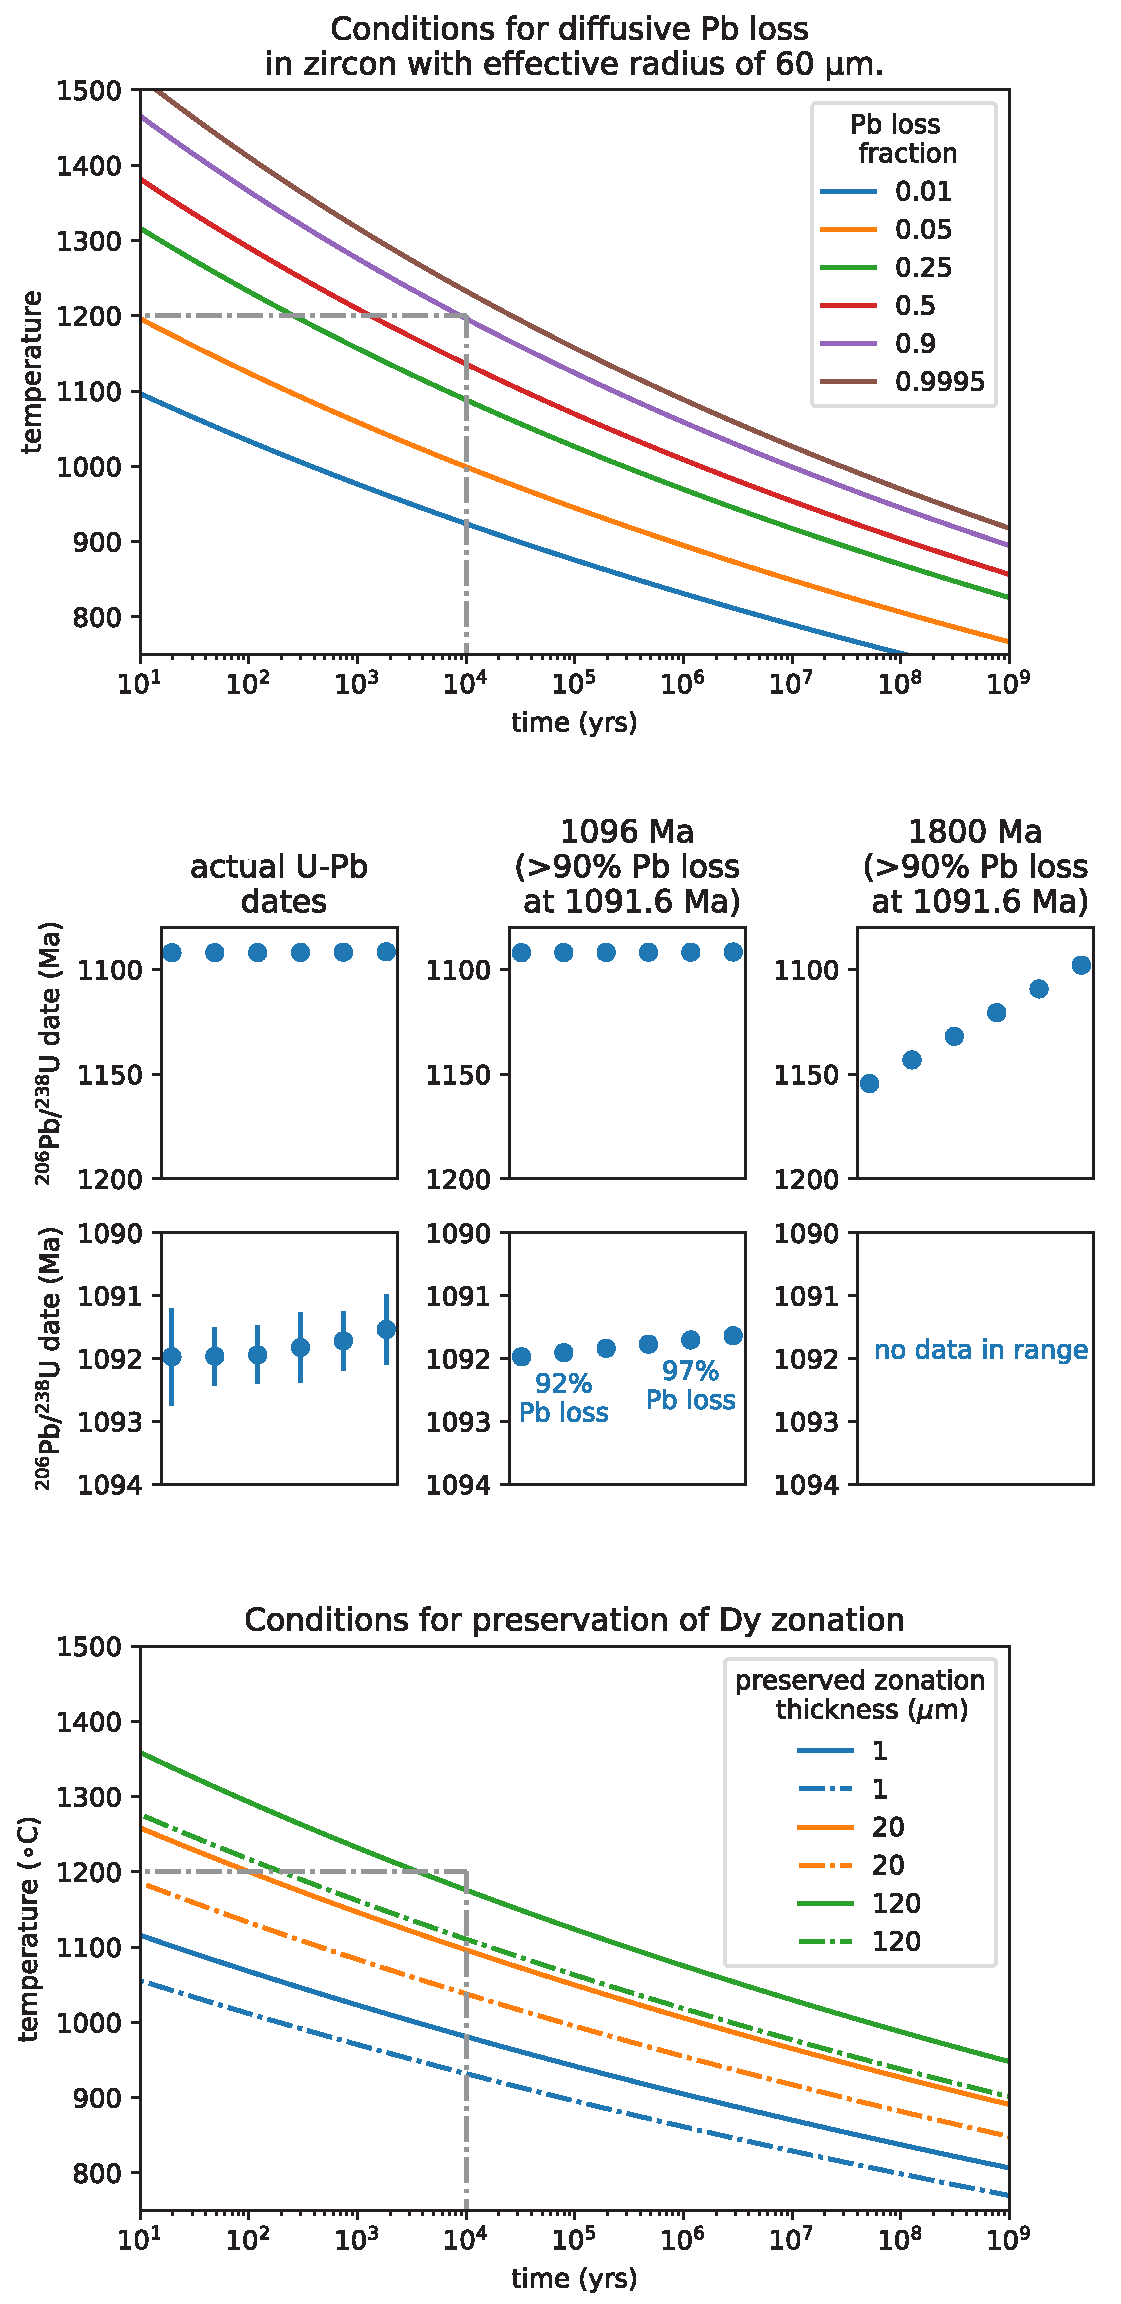
\includegraphics[width=0.47\textwidth]{figure/Zhang2021/diffusive_loss.pdf}
\centering
\caption[Zircon diffusion modeling]{\footnotesize{Top: Conditions for diffusive Pb loss in crystalline zircon for zircons of effective radii of 60 $\mu$m. Curves represent time--temperature conditions under which zircon will lose the indicated fraction of total Pb. Middle: Modeled zircon Pb loss scenarios with initial crystallization ages of 1091.8 Ma, 1096 Ma, and 1800 Ma with varying degrees of Pb loss at 1091.6 Ma compared to the actual U-Pb dates. Bottom: Conditions for preservation of Dy zoning in zircon. Curves represent time-temperature conditions under which different zoning thicknesses would be preserved in zircon. For conditions above the upper solid curves in each group, well-defined zoning will be lost at a given thickness. For conditions above the dashdot lines, zones will be partially lost but will retain initial composition in zone center. Pb diffusion and Dy zoning models follow \cite{Cherniak2001a} and \cite{Cherniak1997a}.}}
\label{fig:diffusive_loss}
\end{figure}

The magnitude of Pb diffusion is dependent on the time spent at such a temperature. Using the diffusion parameters of \cite{Cherniak2001a}, a sustained temperature of 1200\textdegree C for $\sim$10 thousand years is required for diffusive loss of $\sim$90\% of Pb from a $\sim$120 $\mu$m diameter zircon. In this case, zircons that crystallized at 1096 Ma and then lost $>$90\% of their Pb at 1091.6 Ma could give apparent U-Pb dates of 1091.8 Ma that are reproducible at the measurement resolution (Fig. \ref{fig:diffusive_loss}). However, CL imagery reveals sharp boundaries between zones of differing CL response (Fig. \ref{fig:CL_image}) on the scale of $\sim$2 $\mu$m. Such CL zoning patterns are dominantly attributed to concentration variations in the rare earth element Dy \citep{Remond1992a}. A time-temperature history that results in 90\% Pb diffusion out of a 120 $\mu$m diameter zircon would also cause Dy re-equilibration throughout a zircon, leaving no clear zonation (Fig. \ref{fig:diffusive_loss}; \citealp{Cherniak1997a}). Therefore, a scenario where the zircons first crystallized during Duluth Complex magmatism and subsequently lost more than 90\% of Pb is exceedingly difficult to reconcile with the preservation of such thin, sharp zones. In fact, preservation of REE zoning in these zircons limits heating at the emplacement temperatures of the Beaver River diabase to a duration more consistent with our modeled duration of $\sim$100 years of heating prior to cooling to the temperatures that preserve such zonation (Fig. \ref{fig:thermal_history_model}, \ref{fig:diffusive_loss}). It is therefore most probable that the Beaver River diabase anorthosite xenoliths are entrained cumulate enclaves that formed at the time of Beaver Bay Complex magmatism. 

\subsection{A comagmatic relationship between the Beaver River diabase and the Greenstone Flow}

Given the existence of many anorthosite xenoliths whose short-axis diameters often reach tens of meters and can be as wide as 180 meters (Fig. \ref{Chap_BBC_Geologic_map}; \citealp{Boerboom2004a, Boerboom2006b}), the Beaver River diabase magma conduits must have been at least this wide during magma ascent. It would be consistent with such wide conduits extending to hypabyssal depths for magma that flowed through these conduits to have vented to the surface.
 
 \begin{figure}[h!]
\centering
\noindent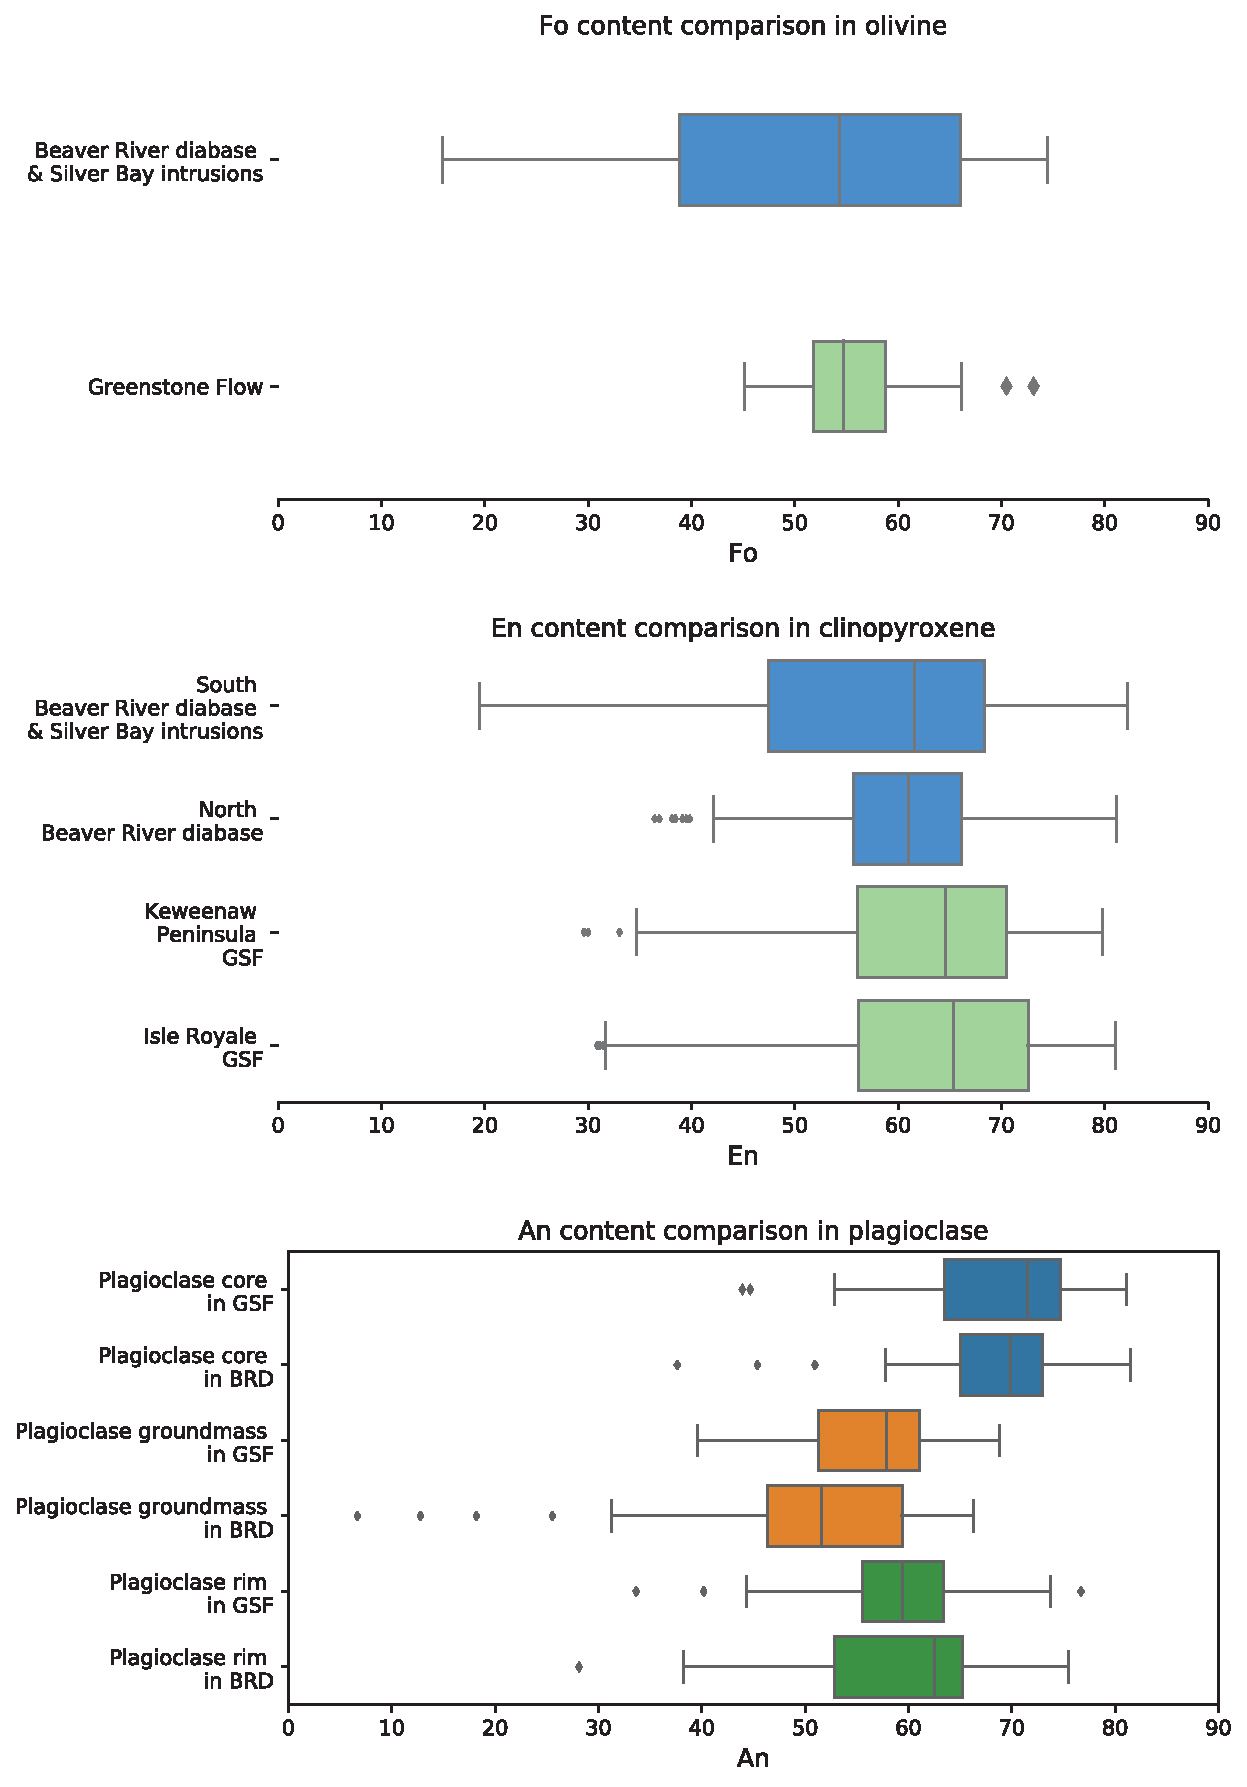
\includegraphics[width=0.68\textwidth]{figure/Zhang2021/Geochem.pdf}
\caption[Box plots of geochemical analyses of olivine, pyroxene, and plagioclase in the Beaver River diabase (BRD) and Greenstone Flow (GSF).]{\footnotesize{Box plots of geochemical analyses of olivine, pyroxene, and plagioclase in the Beaver River diabase (BRD) and Greenstone Flow (GSF). The forsterite content in olivine crystals and the enstatite content in clinopyroxene crystals are very similar in the Beaver River diabase and the Greenstone Flow. The anorthite concentrations in the core, groundmass, and rim of the plagioclase megacrysts within the Beaver River diabase and the Greenstone Flow share very similar patterns and the distributions are nearly identical. The box encloses the middle 50\% of the data ranges (i.e., the interquartile range), and the notch represents the median values. The whiskers extend to the 2.5th and 97.5th percentile values. Fo-forsterite; En-enstatite; An-anorthite. Data from \cite{Doyle2016a}.}}
\label{fig:Geochem}
\end{figure}

The high volume of the extrusive Greenstone Flow of the Portage Lake Volcanics lead to a potential match for this large feeder system. \cite{Doyle2016a} proposed a comagmatic link between the Beaver River diabase and the Greenstone Flow. \cite{Doyle2016a} discovered that both the intrusive Beaver River diabase and the Greenstone Flow have indistinguishable primary compositions that followed similar differentiation patterns. \cite{Doyle2016a} also highlighted the shared petrographic textures between the ophitic Beaver River diabase and the ophitic Greenstone Flow, which features the plagioclase laths clustering together and joining along their long crystallographic axes. The forsterite content of the olivines and enstatite content of the pyroxenes in the Beaver River diabase together with the Silver Bay intrusions, and the Greenstone Flow have overlapping compositions consistent with the same magma source (Fig. \ref{fig:Geochem}). The composition of the plagioclase within the units further strengthens this interpretation. Although there are no known multi-crystalline anorthosite xenoliths in the Greenstone Flow, plagioclase megacrysts occur in the lava flow. Analyses of the anorthite content from plagioclase megacrysts show very similar values between the Beaver River diabase and the Greenstone Flow basalt (Fig. \ref{fig:Geochem}; \citealp{Doyle2016a}). In both units, the plagioclase cores are more enriched in anorthite than the rim and the groundmass. These data provide evidence that the core of the plagioclase megacrysts in the Greenstone Flow derived from a similar source with those in the Beaver River diabase and that the rims are later overgrowths. These mineralogical similarities are consistent with the interpretation that the Beaver River diabase and the Greenstone Flow have the same magma source. 


The synchroneity between the Beaver River diabase and the Greenstone Flow inferred from comparable lithologies and geochemistry can be further evaluated using the paleomagnetic pole positions and radioisotopic dates from both units (Fig. \ref{fig:Direction_pairs}, \ref{fig:BBC_geochron}). The heat diffusion model of the cooling history of the anorthosite xenoliths within the diabase suggests that the time it takes to cool the diabase and anorthosite from low-titanium titanomagnetite Curie temperature ($\sim$580\textdegree C) to their blocking temperatures ($\sim$500\textdegree C) is on the time scale of a few thousand years (Fig. \ref{fig:thermal_history_model}). This time scale is close to the typical 10$^4$ years which is considered to be sufficient for averaging out secular variations of the geomagnetic field. Fig. \ref{fig:Direction_pairs} shows the site mean paleomagnetic pole positions from all diabase and anorthosite sites in this study against the previously synthesized Laurentia APWP developed using an Euler pole inversion to chronostratigraphically constrained volcanic poles in present-day coordinates \citep{Swanson-Hysell2019a}. The site-mean pole positions of the diabase and anorthosite overlap within uncertainty ellipses and the mean pole positions fall between the 1095 Ma and 1090 Ma pole path positions (Fig. \ref{fig:Direction_pairs}), consistent with the geochronology results (Fig. \ref{fig:BBC_geochron}). Further, the mean paleomagnetic pole position derived from the Greenstone Flow share a common mean with those of the Beaver River diabase and the anorthosite xenoliths, but these poles do not share a common mean with the mean pole derived from the Portage Lake Volcanics (Fig. \ref{fig:Direction_pairs}; \citealp{Swanson-Hysell2019a}). This result suggests that the timescale over which the Beaver River diabase and the Greenstone Flow acquired their magnetization may be too short to fully average out secular variation. In this case, the overlapping pole positions between the Beaver River diabase and the Greenstone Flow strengthens their temporal correlation even more (Fig. \ref{fig:Direction_pairs}). 

\begin{figure}[h!]
\centering
\noindent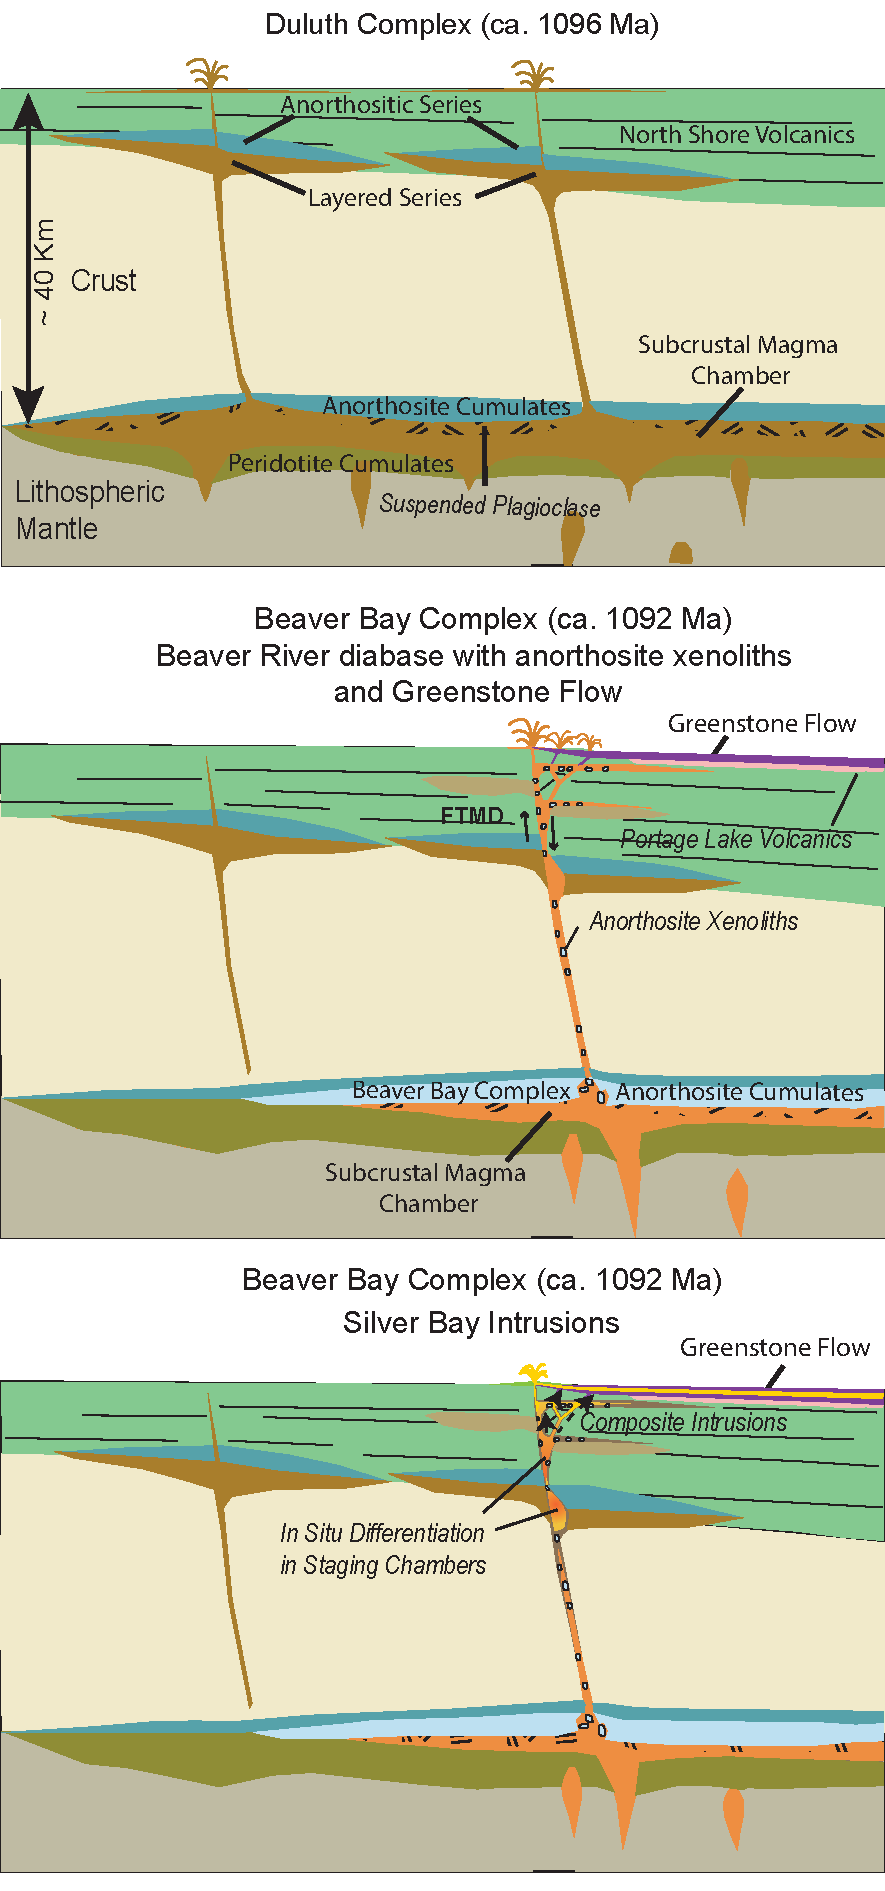
\includegraphics[width=0.4\textwidth]{figure/Zhang2021/Flank_eruption.pdf}
\caption[Schematic illustration of the emplacement of the ca. 1096 Ma Duluth Complex, the ca. 1092 Ma Beaver Bay Complex, Greenstone Flow and associated anorthositic lithologies]{\footnotesize{Schematic illustration of the emplacement of the ca. 1096 Ma Duluth Complex, the ca. 1092 Ma Beaver Bay Complex, Greenstone Flow and associated anorthositic lithologies. Top: Duluth Complex Anorthositic Series formed by subhorizontal emplacement of plagioclase crystal mushes generated by plagioclase flotation in subcrustal magma chambers. The Layered Series formed by emplacement of crystal-poor mafic magmas beneath the Anorthositic Series and variable differentiation by in situ fractional crystallization. Middle: Development of a deep crustal magma chamber that formed anorthosite cumulates and intrusion of the anorthosite xenolith-bearing Beaver River diabase of the Beaver Bay Complex along a major crustal fault (FTMD-Finland Tectonomagmatic Discontinuity) and its massive eruption at surface that could have formed the Greenstone Flow. Bottom: Emplacement of the Beaver River diabase and the Greenstone Flow. The Silver Bay intrusion may have added to the composite composition of both units, through magma differentiation in deeper staging chambers. The erosional unconformity between the Schroeder-Lutsen basalt and the Beaver River diabase suggest the diabase was emplaced into an uplifted rift flank highland which would have led to flank eruptions into the main Midcontinent Rift basin.}}
\label{fig:Flank_eruption}
\end{figure}

The U-Pb dates are consistent with a comagmatic relationship as they reveal indistinguishable ages for the Beaver River diabase and the Greenstone Flow. The age of the Beaver River diabase is constrained to be between the $^{206}$Pb/$^{238}$U dates of  1091.83 $\pm$ 0.21 Ma and 1091.61 $\pm$ 0.14 Ma (Fig. \ref{fig:BBC_geochron}) giving an age estimate of 1091.7 $\pm$ 0.2 Ma (95\% CI). This age is indistinguishable with the $^{206}$Pb/$^{238}$U date of 1091.59 $\pm$ 0.27 Ma for the Greenstone Flow (Fig. \ref{fig:BBC_geochron}).

The Portage Lake Volcanics, including the Greenstone Flow, are interpreted to have erupted into the main central graben of the Midcontinent Rift during an interval of significant subsidence (Fig. \ref{fig:Flank_eruption}; \citealp{Miller1997a,Cannon1992b}). In contrast to the thick accumulation in the Portage Lake Volcanics, the Beaver Bay Complex has an erosional (and slightly angular) unconformity atop it that is then covered by the younger Schroeder-Lutsen basalt (Fig. \ref{Chap_BBC_Geologic_map}; \cite{Miller2001a}). This relationship suggests that the Beaver River diabase was emplaced into a rift flank highland that experienced uplift during the active development of the central graben \citep{Swanson-Hysell2019a}. Eruptions fed through the Beaver River diabase network would have emerged from the rift flank and flowed from the highland into main rift basin (Fig. \ref{fig:Flank_eruption}). 

The proposed intrusive-extrusive connection between the Beaver River diabase and the Greenstone Flow would imply that the Greenstone Flow extended for more than 250 km from northeastern Minnesota to the northern end of Isle Royale where the flow is $\sim$100 m thick and to the northeastern end of the Keweenaw Peninsula, where the flow is $\sim$400 m thick (Fig. \ref{Chap_BBC_Geologic_map}). With this length, the full volume of the Greenstone Flow reaches $\sim$6000 km$^3$ \citep{Doyle2016a}, rivaling the largest known lava flows on Earth (Fig. \ref{fig:lava_flow_rank}). Such lengths were achieved for multiple high volume flows within the Columbia River basalts \citep{Reidel2013a} and are modest compared to the Rajahmundry Trap lavas of the Deccan Traps which traveled $\sim$1000 km \citep{Self2008a}. One potential challenge for a flow having traveled from the Beaver River diabase to the Portage Lake Volcanics is that a reconstruction of present-day rift basin isopachs from seismic data indicates that there is a deep bowl-shaped volcanics-filled basin offshore of Minnesota and the Beaver Bay Complex \citep{Stewart2018a}. While this basin has a thicker accumulation of volcanics than surrounding regions, it is unclear whether it was a topographic barrier. If it was, it could have prevented lavas from present-day northern Minnesota from reaching the portion of the basin now exposed on the Keweenaw Peninsula. Therefore, it is also possible that the indistinguishable ages and similar geochemistry between the Beaver River diabase and the Greenstone Flow are the result of them having been derived from a contemporaneous deep magmatic source without being connected on the surface. 

\section{Conclusion}

There was voluminous emplacement of magma into the shallow subsurface and eruption into the Midcontinent Rift basin ca. 1091.7 Ma at the end of the main stage of Midcontinent Rift volcanism. The anorthosite xenoliths within the Beaver River diabase and their U-Pb geochronology, whose interpretation is informed by REE patterns, indicate that there was a contemporaneous deep crustal magmatic system in which flotation of plagioclase formed anorthosite cumulates. The large dimension of the anorthosite xenoliths require that conduits feeding magma to the surface had widths that exceeded 150 meters. These conduits would have delivered a high volume of magma into the rift basin. The high-precision U-Pb dates, together with paleomagnetic and geochemical data, are consistent with the hypothesis that the Beaver River diabase was the  feeder system of the Greenstone Flow although they could have been disconnected at the surface and both be emblematic of this high-volume pulse of magmatism..

\section{Acknowledgments}
Project research was supported by NSF CAREER grant EAR-1847277 to Nicholas L. Swanson-Hysell and an Institute on Lake Superior Geology Student Research Fund grant to Yiming Zhang. Permits for fieldwork and sampling from the Minnesota Department of Natural Resources are gratefully acknowledged. The authors thank James Pierce and Blake Hodgin for assistance in the field. The authors thank Stephen Self for providing constructive comments regarding mafic lava flow volumes. We thank John Grimsich and Tim Teague at UC Berkeley EPS department for their help with petrographic sample preparation and analyses. We thank U.S. Geological Survey reviewer Jonathan Hagstrum and journal reviewers Bernie Housen and William Rose for their constructive comments on the manuscript.

\chapter[High geomagnetic field intensity recorded by anorthosite xenoliths requires a strongly powered late Mesoproterozoic geodynamo][Late Mesoproterozoic geodynamo]{High geomagnetic field intensity recorded by anorthosite xenoliths requires a strongly powered late Mesoproterozoic geodynamo}

\let\thefootnote\relax\footnote{This chapter is published as a peer-reviewed manuscript: Zhang, Y., Swanson-Hysell, N.L., Avery, M.S., Fu, R.R., (2022), High geomagnetic field intensity recorded by anorthosite xenoliths requires a strongly powered late Mesoproterozoic geodynamo. PNAS. doi: \url{https://doi.org/10.1073/pnas.2202875119}.}

\section{Abstract}
Obtaining estimates of Earth's magnetic field strength in deep time is complicated by non-ideal rock magnetic behavior in many igneous rocks. In this study, we target anorthosite xenoliths that cooled and acquired their magnetization within ca. 1092 Ma shallowly emplaced diabase intrusions of the North American Midcontinent Rift. In contrast to the diabase which fails to provide reliable paleointensity estimates, the anorthosite xenoliths are unusually high-fidelity recorders yielding high-quality, single-slope paleointensity results that are consistent at specimen and site levels. An average value of $\sim$83 ZAm$^2$ for the virtual dipole moment from the anorthosite xenoliths, with the highest site-level values up to $\sim$129 ZAm$^2$, is higher than that of the dipole component of Earth's magnetic field today and rival the highest values in the paleointensity database. Such high intensities recorded by the anorthosite xenoliths require the existence of a strongly powered geodynamo at the time. Together with previous paleointensity data from other Midcontinent Rift rocks, these results indicate that a dynamo with strong power sources persisted for more than 14 million years ca. 1.1 Ga. These data are inconsistent with there being a progressive monotonic decay of Earth's dynamo strength through the Proterozoic Eon and could challenge the hypothesis of a young inner core. The multiple observed paleointensity transitions from weak to strong in the Paleozoic and the Proterozoic present challenges in identifying the onset of inner core nucleation based on paleointensity records alone. 


\section{Introduction}
Earth's magnetic field is the result of convective flow of liquid iron-alloy in Earth's outer core. At present day, the geodynamo is collectively powered by heat flow across the core-mantle boundary (CMB) and from the crystallization of the solid inner core from the liquid outer core which provides latent heat and compositional buoyancy due to the exclusion of light elements \citep{Buffett2000a}. However, while paleomagnetic studies have found that a dynamo field has existed since at least 3.4 billion years ago \citep{Selkin2007a, Biggin2011a, Tarduno2014a, Brenner2020a}, Earth's inner core likely crystallized more recently. Estimates of the timing of the initial crystallization of Earth's inner core are interconnected with estimates for the core's thermal conductivity. Higher conductivity values imply faster cooling rates to maintain the geomagnetic field, which in turn imply that the threshold for the crystallization of the inner core happened more recently \citep{Davies2015a}. While some estimated thermal conductivity values are consistent with an inner core age $>$3 Ga \citep{Gubbins2004a, Konopkova2016a}, other estimates have implied higher thermal conductivity values and an age for the inner core that is less than 1.5 Ga \citep{Pozzo2012a, Koker2012a, Gomi2013a, Zhang2020b, Frost2022a}, with some suggesting even younger ages ($<$700 Ma; \citealp{Labrosse2015a, Ohta2016a, Pozzo2022a}). The possibility of late inner core nucleation has motivated proposals of novel power sources to sustain the geomagnetic field through early Earth history including precipitation of light-element minerals such as MgO \citep{Badro2016a, ORourke2016a, ORourke2016b} and SiO$_2$ \citep{Mittal2020a} at the core-mantle boundary. Given that estimates for the core's thermal conductivity continue to be debated, it is crucial to use observational records as an independent constraint on the thermal evolution of Earth's core and mantle.

Paleomagnetic records from ancient rocks are one of the few types of observational data that have the potential to provide constraints on the thermal evolution of Earth’s core. Evidence for a persistent magnetic field through the Proterozoic, for example, likely necessitates the existence of plate tectonics that sustained core-mantle boundary heat flow \citep{Swanson-Hysell2021c}. However, strikingly low estimates of geomagnetic field strengths have been obtained ca. 565 Ma during the Ediacaran Period \citep{Bono2019a, Shcherbakova2019a,Thallner2021b} and ca. 370 Ma during the Devonian Period \citep{Shcherbakova2017a, Shcherbakova2021a, Hawkins2021a}, potentially indicating unusual periods of core dynamo activity at those times. The Ediacaran data have been interpreted to indicate that there was a progressively decaying field up to that time that was soon followed by initial crystallization of the inner core \citep{Bono2019a}. Sparse paleointensity data in the Proterozoic Era (2500 to 539 Ma) and the reality of high variability in Phanerozoic Era records (539 to 0 Ma) necessitate additional data to evaluate interpreted trends. 

\begin{figure}[h!]
\centering
\noindent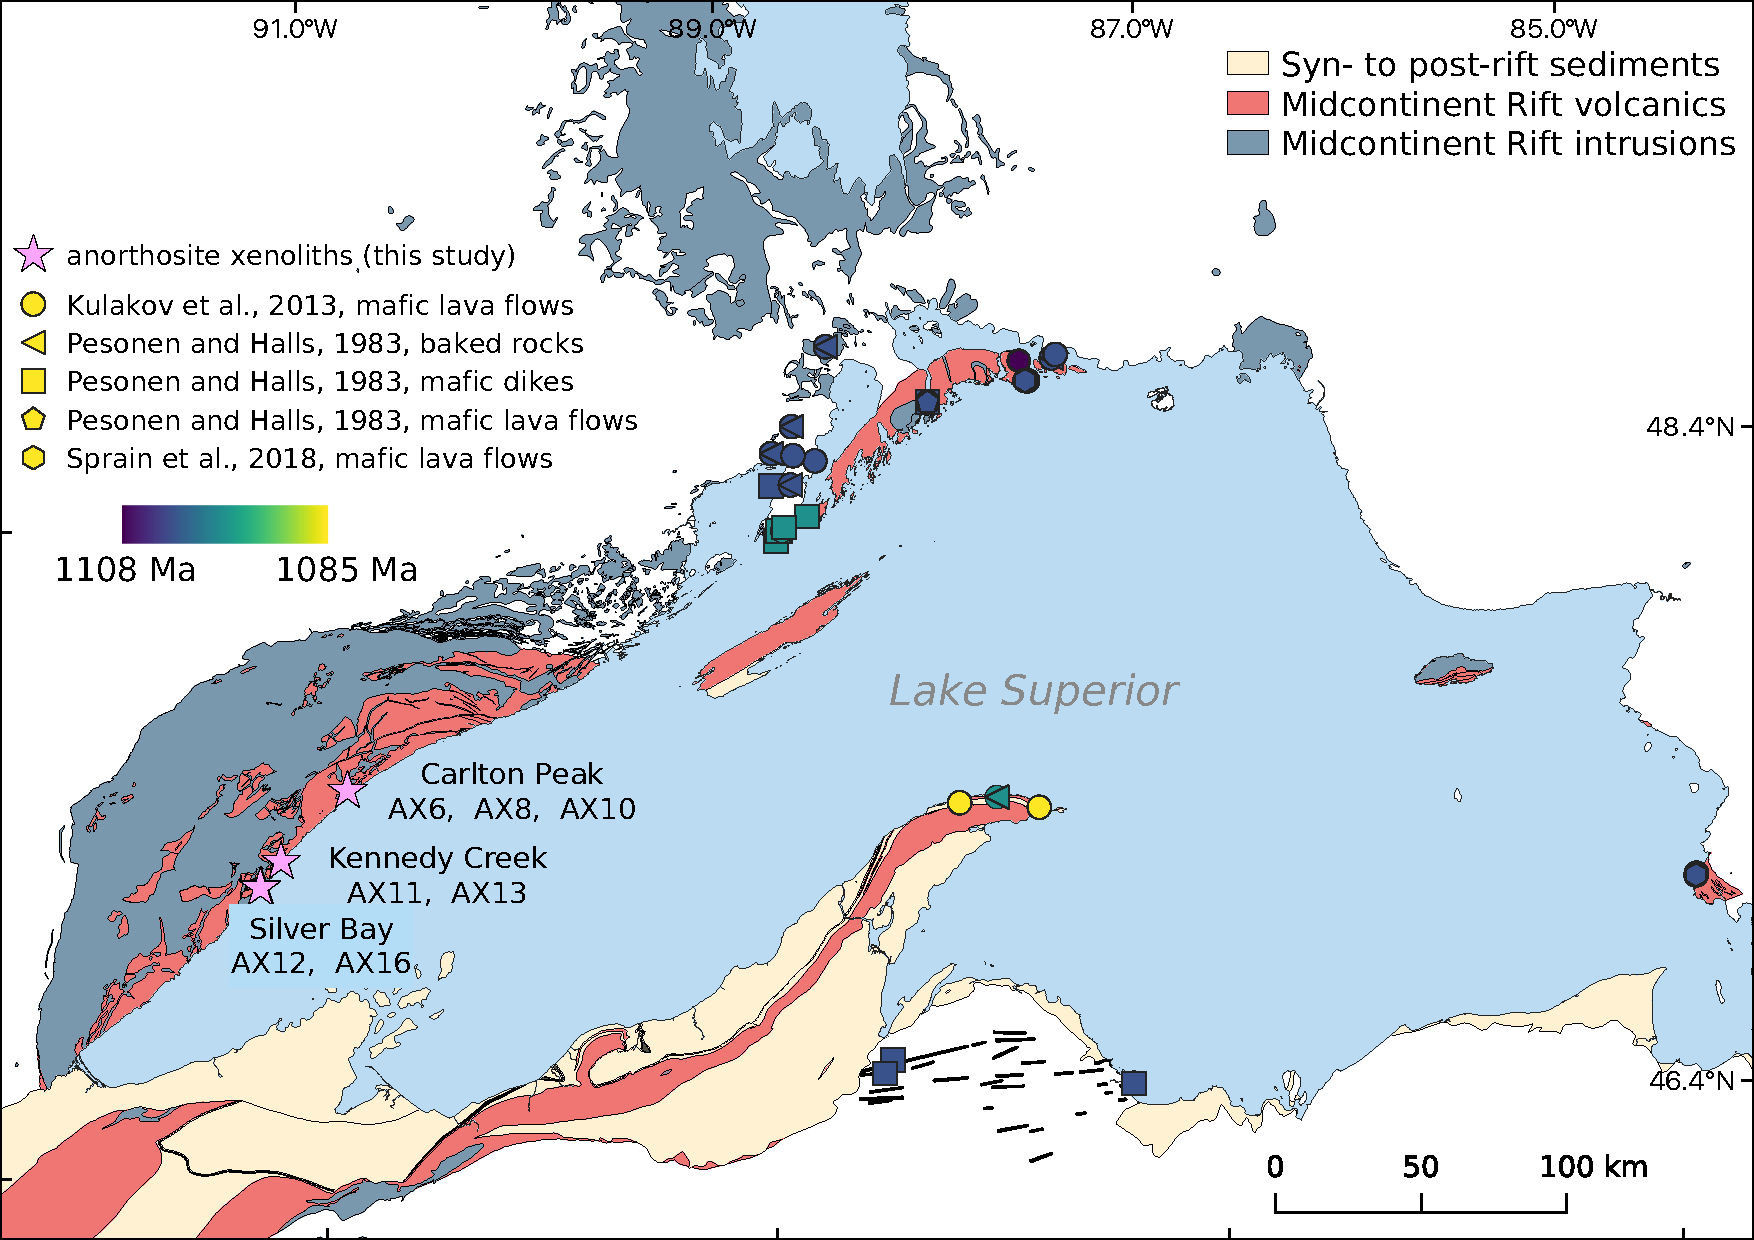
\includegraphics[width=0.9\textwidth]{figure/Zhang2022/Geologic_map.pdf}
\caption[Simplified geologic map of the Lake Superior region]{\footnotesize{Simplified geologic map of the Lake Superior region showing the distribution of rocks associated with the late Mesoproterozoic Midcontinent Rift. Purple stars mark sites with paleointensity results that passed the selection criteria from this study. Paleomagnetic sites from \citealp{Pesonen1983a} are categorized by lithology. All sites from refs. \citealp{Pesonen1983a, Kulakov2013a, Sprain2018a} are color-coded by their ages.}}
\label{fig:Chap_PINT_Geologic_map}
\end{figure}

Determinations of the absolute value of ancient geomagnetic field strength rely on igneous rocks that acquire thermal remanent magnetizations as they cool. These magnetizations need to be unmodified by subsequent heating or chemical alteration in order to maintain the record of the ancient geomagnetic field from the time of cooling. Intracontinental magmatic events are an important target for determination of ancient paleointensity as they can be well-preserved within continental interiors. This interior position results in them typically being distant from tectonic events along continental margins that can drive alteration through heat and fluid flow. However, intraplate magmatism associated with large igneous provinces is typically of geologically short duration with the bulk of magmatic products emplaced within 1 Myr or less \citep{Kasbohm2021a}. The Midcontinent Rift (Fig. \ref{fig:Chap_PINT_Geologic_map}) is an exception as it is a large igneous province where magmatism lasted $\sim$25 Myr from ca. 1109 Ma to 1084 Ma during which there were pulsed intervals of more rapid magmatic activity \citep{Swanson-Hysell2021a}. Additionally, extension ceased in the Midcontinent Rift prior to lithospheric separation, preserving volcanic, intrusive, and sedimentary rocks of the rift within the continental interior far from the continental margin and subsequent orogenesis. As a result, rocks of the rift have unusually simple paleomagnetic behavior for their greater than one billion-year-old age and paleomagnetic data from rift rocks form a central record of Mesoproterozoic paleogeography \citep{Swanson-Hysell2021c}. The duration of magmatic activity within the Midcontinent Rift is longer than the entire 20.4 Myr long Neogene Period such that it provides an extended well-preserved window into the intensity of Earth's magnetic field in the late Mesoproterozoic. 

Despite the excellent preservation of the rocks, non-ideal paleointensity behaviors have posed challenges for the interpretation of many previous paleointensity results from the Midcontinent Rift \citep{Pesonen1983a, Kulakov2013a, Sprain2018a}. The most trusted type of paleointensity estimate is that obtained through experiments in which the primary natural remanent magnetization (NRM) is progressively replaced by a laboratory magnetization that is imparted in a known field with internal consistency checks (such as in IZZI-style Thellier experiments;  \citealp{Yu2004a}). In such Thellier paleointensity experiments, one typical departure from ideal behavior due to the presence of nonuniformly magnetized grains (with either multidomain \citep{Dunlop2001a} or vortex states \citep{Tauxe2020a}) is sagging or double-slopes as visualized in Arai plots that show thermal remanent magnetization (TRM) acquired versus NRM lost. For such data, distinct paleointensity estimates may be calculated depending on the interpreter's choice of slope. Typically, such non-ideal behavior would result in a higher paleointensity estimate from the steeper-sloped low-temperature portion of the experiment and a lower paleointensity estimate from the high-temperature portion. For example, in data from the Midcontinent Rift, \cite{Pesonen1983a} used the low-temperature slope as the best representation of the past magnetic field strength (likely overestimating the field strength) whereas \cite{Kulakov2013a} used the high-temperature slope (likely underestimating the field strength). Such non-ideal results were rejected by \cite{Sprain2018a} who applied stricter paleointensity selection criteria, but as a result had few accepted sites.

In this study, we target the high-purity anorthosite xenoliths of the Beaver River diabase in the Midcontinent Rift. While magmatic activity within the Midcontinent Rift was protracted, there were intervals of particularly rapid volcanism and voluminous emplacement of intrusions \citep{Swanson-Hysell2021a}. The ca. 1092 Ma Beaver Bay Complex in northern Minnesota punctuates one such period of magmatism during the main stage of Midcontinent Rift activity. The magma that formed the 1091.7 $\pm$ 0.2 Ma Beaver River diabase dikes and sills of the Beaver Bay Complex transported numerous anorthosite xenoliths that have short-axis diameters up to 180 meters via wide conduits \citep{Boerboom2004a, Boerboom2006b}. These anorthosite xenoliths are plagioclase cumulates that formed comagmatically with the host diabase in the lower crust---an interpretation confirmed by U-Pb zircon geochronology \citep{Zhang2021b}. They are attractive targets for paleomagnetic study as plagioclase crystals can protect magnetic inclusions from alteration. In addition, the alteration of the plagioclase crystals does not readily result in the formation of secondary iron oxides in contrast with Fe-silicate minerals such as olivine and pyroxene. The anorthosite xenoliths targeted in this study were brought to the near surface in magma that formed hypabyssal (shallowly emplaced) intrusions of the Beaver River diabase \citep{Zhang2021b}. They would have been heated to tholeiitic magma temperature ($\sim$1100\textdegree C) which is below the melting point of the xenolith plagioclase (70$\%$ anorthite), but well above the Curie temperature of magnetite \citep{Zhang2021b}. Fe-Ti oxides within the plagioclase likely exsolved above magnetite Curie temperature \citep{Bian2021a} and subsequently cooled and acquired thermal remanent magnetizations in conjunction with the host diabase at a paleolatitude of 22 $\pm$ 2\textdegree$\;$(calculated from the paleomagnetic pole of the coeval Portage Lake Volcanics; \citealp{Swanson-Hysell2019a}). Paleointensity experiments on the anorthosite xenoliths have a high success rate, yielding consistent specimen- and site-level paleointensity results. The anorthosite xenoliths show low anisotropy of thermal remanent magnetization acquisition and can acquire TRM linearly within the range of relevant field strengths. Magnetic imaging shows that the anorthosite specimens have dominant magnetic carriers within and interstitial to plagioclase crystals without strong preferred orientations. Thermal modeling results and paleomagnetic directional data show that the anorthosite xenoliths acquired thermal remanent magnetizations while cooling with the Beaver River diabase \citep{Zhang2021b}. Step-wise thermal demagnetization data show the anorthosite xenoliths to have dominantly single-component magnetizations that often unblock sharply within temperature ranges between 500\textdegree C and 580\textdegree C, consistent with remanence being held by low-titanium titanomagnetite \citep{Zhang2021b}. 

\begin{SCfigure*}
\centering
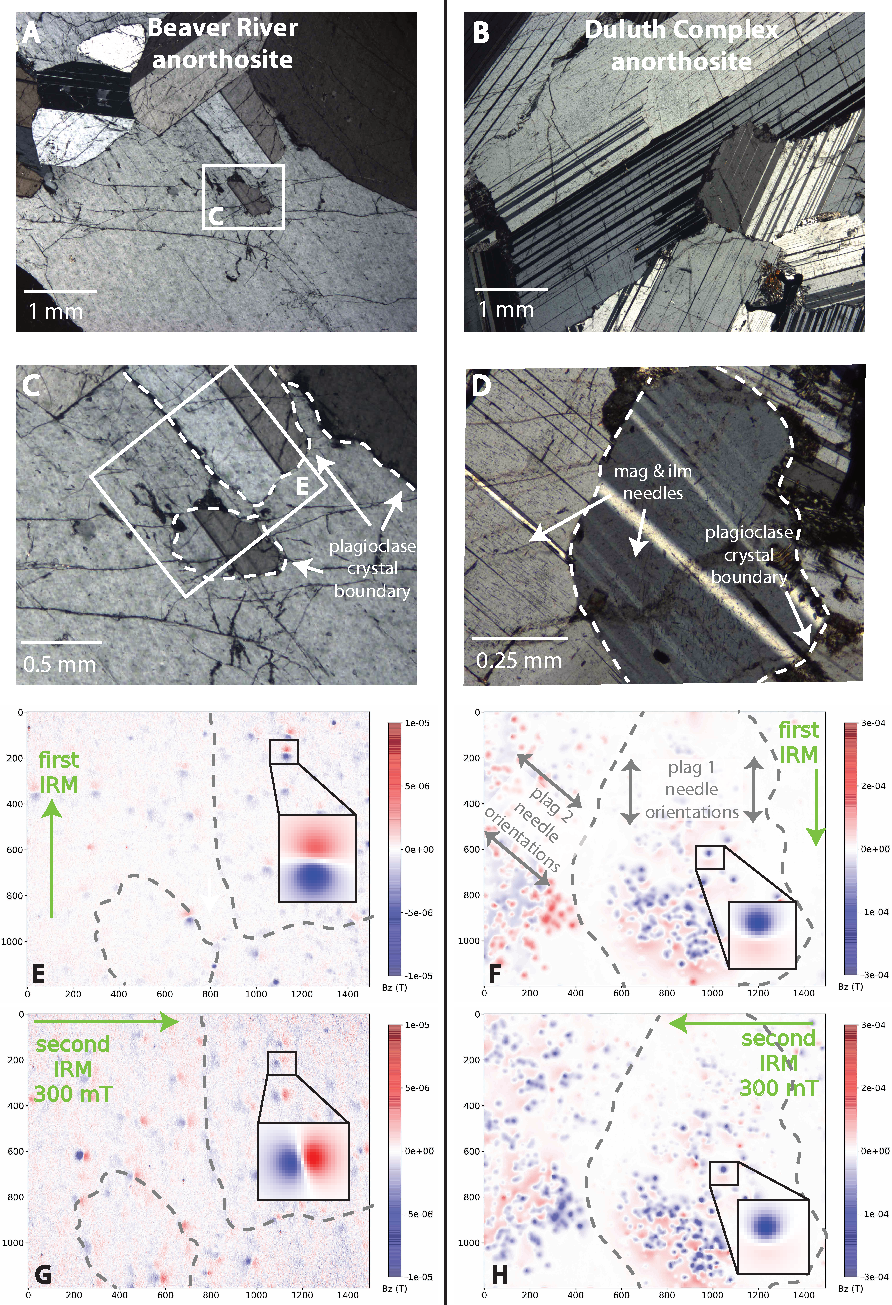
\includegraphics[width=0.6\textwidth]{figure/Zhang2022/Petro_QDM_full.pdf}
\caption[Petrographic images and magnetic field maps of anorthosite samples from the Beaver Bay Complex and the Duluth Complex]{\tiny Thin section petrographic images (A,B,C,D) and magnetic maps (E,F,G,H) of an anorthosite sample from the Beaver River anorthosite xenolith in the Silver Bay region from which paleomagnetic site AX16 and geochronology sample MS99033 were collected (left column;  \citealp{Zhang2021b}) and from a distinct anorthosite within the Duluth Complex Anorthositic Series (right column). The Duluth Complex anorthosites were not targeted for paleointensity experiments in this study given complexities associated with more pronounced fabrics. Cross-polarized petrographic images of the Beaver River anorthosite (A,C) reveal plagioclase with a granoblastic texture of crystals that are largely free of large opaque inclusions. In contrast, plagioclase crystals in the Duluth Complex anorthosite have euhedral, interlocking crystals with an igneous foliation (B) and the plagioclase crystals contain abundant Fe-Ti oxide needles that have preferred orientations that are often parallel with the [001] axis of the plagioclase. Maps of the vertical component of magnetic field (B$_z$) developed with a quantum diamond microscope (QDM) show relatively weak magnetic sources within plagioclase crystals in the Beaver River anorthosite (in E) relative to the strongly magnetic large oxide needles within Duluth Complex plagioclase (in F). The B$_z$ color scale is an order of magnitude greater in the Duluth Complex anorthosite maps (F, H) than the maps for the Beaver River anorthosite (E, G). Panels (E) to (G) and (F) to (H) show experiments performed on both samples where we apply a first field along the y-axis of the field of view and then apply a second field of 300 mT orthogonal to the first field direction. The remanent magnetizations acquired by both anorthosites were mapped after the application of each field. The magnetic images show that remanent magnetizations of Beaver River anorthosite (i.e. the individual dipoles visible with paired red +B$_z$ and blue -B$_z$ lobes) align well with the first applied field direction (E) and then rotated to align with the second applied field direction indicating minimal anisotropic behavior (G). In contrast, the remanent magnetizations carried by the magnetic needles in plagioclase 1 of the Duluth anorthosite xenolith align well with the first applied field but those in plagioclase 2 acquired an oblique remanence direction with respect to the field direction (F). After the application of an orthogonal 300 mT external field, magnetization of those needles in plagioclase 1 did not change direction due to strong shape anisotropy whereas the magnetization of needles in plagioclase 2 flipped, but with the acquired remanence remaining oblique to the field direction (H). Insets in (E) to (H) show example dipole directions (fit using the algorithm of \citealp{Lima2016a}) in response to the application of orthogonal IRMs. The directional changes of the Beaver River anorthosite xenolith sources indicate a lower magnetic anisotropy compared to the relative lack of change for the Duluth Complex anorthosite xenolith sources. The unit of the axes in the QDM maps are in $\mu$m.}
\label{fig:Petro_QDM}
\end{SCfigure*}

\section{Methods}
\subsection*{Sample collection and paleomagnetic directions}

We collected paleomagnetic cores that are 2.5 cm in diameter along the southern and eastern Beaver Bay Complex with a particular focus on acquiring paired sites of anorthosite xenoliths and their local diabase hosts during summer field seasons in 2019 and 2020. Sample cores were collected using a hand-held gasoline-powered drill and were oriented using a magnetic compass as well as a sun compass when possible. Sun compass orientations were preferentially used for determining the sample azimuth. Sister specimens underwent step-wise alternating field (AF) or thermal demagnetization at the UC Berkeley Paleomagnetism Lab to isolate paleomagnetic directions (data presented in \citealp{Zhang2021b}). Based on the anorthosite thermal demagnetization results, we selected sites whose unblocking temperature ranges are narrow and near 580\textdegree C for paleointensity experiments. Beaver River diabase sites with minimal secondary remanence were also selected for paleointensity experiments. 

\subsection*{Paleointensity experiment}
A total of 86 specimens from 14 anorthosite xenoliths and a total of 69 specimens from 7 diabase sites underwent paleointensity experiments that followed the step-wise double-heating Thellier method \citep{Thellier1959a} using the IZZI protocol \citep{Yu2004a} with heating steps up to 585 \textdegree C. Partial thermal remanent magnetization (pTRM) checks were performed systematically throughout the experiment to test whether there was significant mineralogical alteration due to heating and were assessed using the SCAT parameter of  \citealp{Shaar2013a}. On top of the IZZI-Thellier experiment protocol, we also performed a comparative study where we added an extra step of 20 mT alternating field (AF) cleaning on some of the specimens after each in-field step. The purpose was to study whether the AF cleaning could help improve experiment success rate by removing the remanence component carried by materials such as multi-domain (MD) grains that contribute to non-ideal paleointensity behaviors. The results were similar when this step was applied without an observed change in experimental success rate. All remanence measurements were made on a 2G Enterprises DC-SQUID superconducting rock magnetometer equipped with an automated sample changer system at the UC Berkeley Paleomagnetism laboratory. The magnetometer is housed inside a three-layer magnetostatic shield that maintains background fields of less than 500 nT. Heating steps were performed using an ASC TD-48SC thermal demagnetizer with a controlled field coil that allows for a magnetic field to be generated in the oven in conjunction with a DC power supply. The thermal demagnetizer was degaussed with an alternating field in the axial orientation following each in-field step such that residual fields within the oven were $<$10 nT during zero-field steps. Samples were placed in the same location within the thermal demagnetizer for each heating step and were maintained in the same orientation with regard to the applied field. During each heating step, the oven remained at peak temperatures for 20 min to make sure each specimen reached the target temperature. An applied laboratory field of 30 $\mu$T was used for all in-field steps. All heating steps were performed in air. The temperature increments for the experiments were chosen to isolate magnetizations held by (titano)magnetite informed by the previous demagnetization data, with smaller increments performed close to $\sim$580\textdegree C. 

\subsection*{Paleointensity result selection}
The following criteria were used as quality filters on the paleointensity results: (1) a maximum angular deviation (MAD; \citealp{Kirschvink1980a}) of $<$10\textdegree; (2) scatter parameter ($\beta$; \citealp{Coe1978a}) values of $<$15$\%$; (3) a deviation angle (DANG; \citealp{Tauxe2004a}) of $<$5\textdegree; (4) fraction of remanence fitted for paleointensity estimate (FRAC; \citealp{Shaar2013a}) $>$0.6; (5) scatter statistic (SCAT; \citealp{Shaar2013a}) = TRUE; (6) a maximum magnetic moment difference between adjacent zero-field steps (GAP-Max; \citealp{Shaar2013a}) $<$ 0.25; (7) number of pTRM checks $>$ 2; (8) and number of measurements used for paleointensity determination $\geq$ 4. MAD measures the scatter about the best-fit line through the natural remanent magnetization (NRM) steps in the selected interval for which the intensity is defined. DANG, the deviation angle, is the angle between the best-fit direction that is free floating and the direction between the center of mass of the data and the origin of the vector component diagram \citep{Tauxe2004a}. Both MAD and DANG assess the directional variation of the NRM, with MAD measuring the scatter in the NRM directions and DANG assessing whether the component is trending toward the origin of the Zijderveld plot. $\beta$ is the ``scatter" parameter of \cite{Coe1978a} and is the ratio of the standard error of the slope of the best-fit line of the selected NRM and pTRM points on an NRM/TRM plot to the absolute value of the slope. FRAC is the fraction of the NRM that is used in the best-fit line \citep{Shaar2013a}. The FRAC value was chosen to preferentially select samples with dominantly single-slope NRM/TRM plots. GAP-Max is the maximum gap between two points on the NRM/TRM plot determined by vector arithmetic. SCAT is a Boolean operator which uses the error on the best-fit slope of the selected data on the NRM/TRM plot to determine if the data are overly scattered. The parameter is used to assess pTRM checks in addition to assessing the degree to which IZZI steps are zigzagged. $\beta$, FRAC, GAP-Max and SCAT are all statistics to assess the behavior of NRM/TRM plots. See the Standard Paleointensity Definitions (\citealp{Paterson2014a}; \url{https://earthref.org/PmagPy/SPD/home.html}) for more details. Data analysis was conducted using Thellier GUI \citep{Shaar2013a} within the PmagPy software package \citep{Tauxe2016a}.

\subsection*{Rock magnetic experiments}

We conducted rock magnetic experiments to characterize the magnetic mineralogy and gain insights into the paleointensity results of the anorthosite and diabase. Back-field curves were measured at room temperature using a Micromag Princeton Measurements vibrating sample magnetometer (VSM) and a Lake Shore 8600 series VSM at the Institute for Rock Magnetism. Specimen median destructive fields (MDF) were calculated based on the back-field experiments. The calculated coercivity spectra were subsequently decomposed into one or more components using skew-normal distributions following the method of  \citealp{Maxbauer2016a} examples of which are shown in Fig. \ref{fig:coercivity}. We also used a magnetic property measurement system (MPMS) at the Institute for Rock Magnetism to aid the identification of magnetic minerals. In the field-cooled (FC) experiments, specimen magnetizations were measured upon warming following the specimen having cooled in an applied field of 2.5 T from 300 to 10 K. In the zero-field-cooled (ZFC) experiment, a low-temperature saturation isothermal remanence (LTSIRM) of 2.5 T was applied at 10 K after the specimen cooled in a (near-)zero field. In the room-temperature saturation isothermal remanence (RTSIRM) experiment, the sample was pulsed with a 2.5 T field at room temperature ($\sim$300 K) and then cooled to 10 K and warmed back to room temperature in a (near-)zero field. The magnetic moment transitions at critical temperatures shown through MPMS experiments were used to identify magnetic minerals such as magnetite within specimens \citep{Feinberg2015a}. 

To further identify the magnetic carriers within the Beaver River anorthosite xenoliths and compare them with the anorthosites of the Duluth Complex Anorthositic Series rocks, we used the quantum diamond microscope (QDM) at the UC Berkeley Paleomagnetism laboratory to image a thin section of sample MS99033 from anorthosite xenolith AX16 (which yielded a $^{206}$Pb/$^{238}$U zircon date of 1091.83 $\pm$ 0.21 Ma;  \citealp{Zhang2021b}), and a thin section of a Duluth Complex anorthosite (Fig. \ref{fig:Petro_QDM}). We use the QDM to image the magnetic field over the polished thin section surfaces with a sample-sensor distance of $\sim$5 $\mu$m in projective magnetic microscopy (PMM) mode with a spatial resolution of 4.7 $\mu$m per pixel and an instantaneous 0.9 mT bias field that is canceled during the course of measurement \citep{Glenn2017a}.

\section{Results and Interpretations}

\subsection*{Petrography and magnetic imaging of anorthosite xenoliths}

The dominantly monomineralic anorthosite xenoliths within the Beaver River diabase often have granoblastic texture characterized by equigranular crystals with weakly developed petrofabrics (Fig. \ref{fig:Petro_QDM}A). Plagioclase crystals within coarse-grained intrusions often contain abundant elongate Fe-Ti oxide inclusions that are visible with optical microscopy \citep{Feinberg2006a, Wenk2011a, Ageeva2016a}. The Beaver River anorthosite xenoliths lack such large (10s of $\mu$m) oxide inclusions such that the oxides are not visible within the plagioclase crystals using optical microscopy (Fig. \ref{fig:Petro_QDM}C). Magnetic imaging using a quantum diamond microscope (QDM), however, shows that there are magnetic remanence carriers within the plagioclase crystals (Fig. \ref{fig:Petro_QDM}E, G). The sources of these magnetic remanence carriers are likely to be Fe-Ti oxides that exsolved within plagioclase crystals above the Curie temperature of magnetite \citep{Zhang2021b, Bian2021a}. To highlight these distinctive aspects of the Beaver River anorthosite xenoliths, we present petrographic and magnetic imaging data from the Beaver River anorthosite as well as an anorthosite sample from the Duluth Complex Anorthositic Series---an older intrusive complex within the Midcontinent Rift that was not targeted for paleointensity experiments in this study (Fig. \ref{fig:Petro_QDM}). In contrast to the Beaver River anorthosite, the plagioclase crystals of this Duluth Complex anorthosite sample has a pronounced igneous foliation (Fig. \ref{fig:Petro_QDM}B). In addition, there are abundant Fe-Ti oxide needles within the Duluth Complex plagioclase grains that are typically aligned with the [001] axes of the crystals (Fig. \ref{fig:Petro_QDM}D). Magnetic imaging confirms that these needles have magnetic moments oriented along their long axes (Fig. \ref{fig:Petro_QDM}F, H). As a result of this shape anisotropy, remanent magnetizations are acquired at angles highly oblique to applied fields (Fig. \ref{fig:Petro_QDM}F). In an experiment where a second orthogonal field was applied, the first isothermal remanent magnetizations (IRM) of a set of magnetite needles within a plagioclase grain either fail to rotate or flip by 180\textdegree. When they flip, they remain in a direction that is oblique to the applied field direction dictated by shape anisotropy (Fig. \ref{fig:Petro_QDM}F, H). These experiments enable novel visualization of the grain-scale magnetic anisotropy of elongated exsolved (titano)magnetite inclusions within plagioclase grains that leads to magnetic anisotropy observed at the bulk sample scale \citep{Selkin2000a, Feinberg2006a}. In contrast, the remanent magnetizations of the ferromagnetic grains imaged in the Beaver River anorthosite xenoliths, targeted for paleointensity in this study, align with the applied field directions indicating minimal remanence anisotropy  (Fig. \ref{fig:Petro_QDM}E, G). The relative lack of petrofabrics and minimal grain-scale magnetic anisotropy make the Beaver River anorthosite xenoliths a particularly compelling target for paleointensity experiments.

\subsection*{Paleointensity}

Following IZZI-style paleointensity experiments \citep{Yu2004a}, 40 from a total of 86 anorthosite specimens and 0 out of a total of 69 diabase specimens passed our paleointensity result selection criteria (see Materials and Methods section). Seven anorthosite sites and no diabase sites have specimen results that pass these selection criteria. Example NRM/TRM (Arai) plots are shown in Figure \ref{fig:IZZI_examples}. Summary specimen absolute paleointensity estimates and site-level mean paleointensity values are plotted in Figure \ref{fig:PINT_cooling_corrected} (and provided in Table \ref{tab:PINT_result}) where each site represents an individual anorthosite xenolith. The paleointensity quality index (Q$_{PI}$; \citealp{Biggin2014a}) for the anorthosite xenolith sites are all 5 or 6 (Table \ref{tab:QPI}). The cooling rate-corrected absolute paleointensity estimates from the anorthosite xenoliths have a mean of 38.86 $\pm$ 12.10 $\mu$T. The site-mean virtual dipole moment is $\sim$83 ZAm$^2$ ($10^{21} Am^2$) ca. 1092 Ma. All measurement-level paleointensity experiment data are available within the MagIC database (\url{https://doi.org/10.7288/V4/MAGIC/19462}). 

\begin{figure*}
\noindent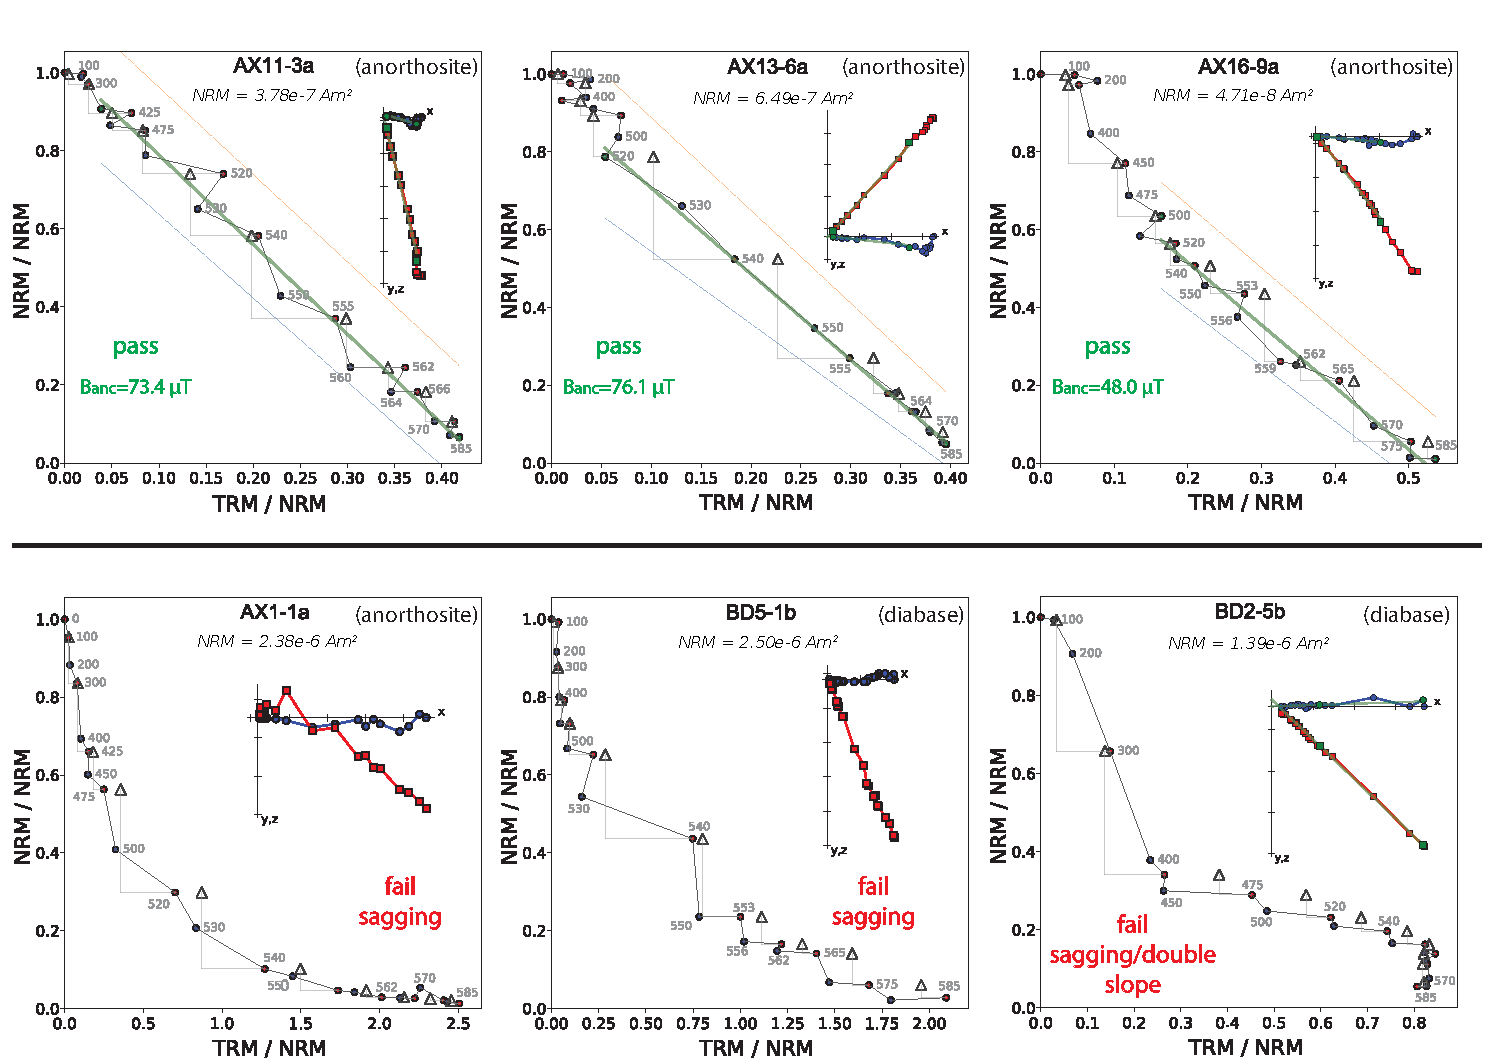
\includegraphics[width=\textwidth]{figure/Zhang2022/IZZI_examples.pdf}
\centering
\caption[Example Arai plots of paleointensity experiment results from Beaver River diabase and anorthosite]{\footnotesize{Example results of paleointensity experiments are displayed on Arai plots and zero-field heating results are shown as inset orthogonal plots (Zijderveld plots) for anorthosite and diabase specimens. Green squares and lines in Arai plots and green squares in orthogonal plots show the range of data points used for fitting. Red (blue) circles indicate zero-field/in-field (in-field/zero-field) steps `ZI'(`IZ'). Triangles mark partial thermal remanent magnetization (pTRM) checks. Blue and red squares in the Zijderveld plots are X–Y and X–Z projections, respectively, of the NRMs in specimen coordinates. Dashed red and blue lines show bounding regions associated with the \textit{SCAT} statistic \citep{Shaar2013a}. Plots on the top row show successful specimen paleointensity results with straight, single-slope behaviors that pass our selection criteria. The green lines represent fits for the dominant single-slope component that passes the acceptance criteria and gives an estimate of the ancient field strength (B$_{anc}$). The plots for anorthosite specimens AX1-1a and diabase BD5-1b on the bottom row show non-ideal sagging behaviour that fails our acceptance criteria. Specimen BD2-5a is an example where the data appear linear with distinct slopes in the low and high temperature ranges such that it could pass less restrictive selection criteria, particularly if a narrower temperature range was used for the experiment. Data analysis and visualization was conducted using PmagPy \citep{Tauxe2016a}.}}
\label{fig:IZZI_examples}
\end{figure*}

Typical paleointensity experimental data of the anorthosite specimens have straight, single-slope NRM/TRM plots and the accepted fractions of temperature steps span over the origin-trending, primary remanence components (Fig. \ref{fig:IZZI_examples}). We accept specimen- and site-level absolute paleointensity results from those anorthosite xenoliths that pass the selection criteria. Other anorthosite xenoliths and diabase specimens failed the selection criteria largely because of double-slope or sagging behavior (fail FRAC selection; see Materials and Methods section), poor pTRM checks, and zigzagging behaviors occasionally superimposed on top of sagging behavior (fail SCAT, DANG selection; see Materials and Methods section; Fig. \ref{fig:IZZI_examples}). A 20 mT alternating field treatment after in-field heating steps was applied to some specimens, but this treatment did not result in significant changes in the experimental results for the anorthosite xenolith or diabase specimens (Fig. \ref{fig:PINT_cooling_corrected}). 

\begin{figure*}[h!]
\noindent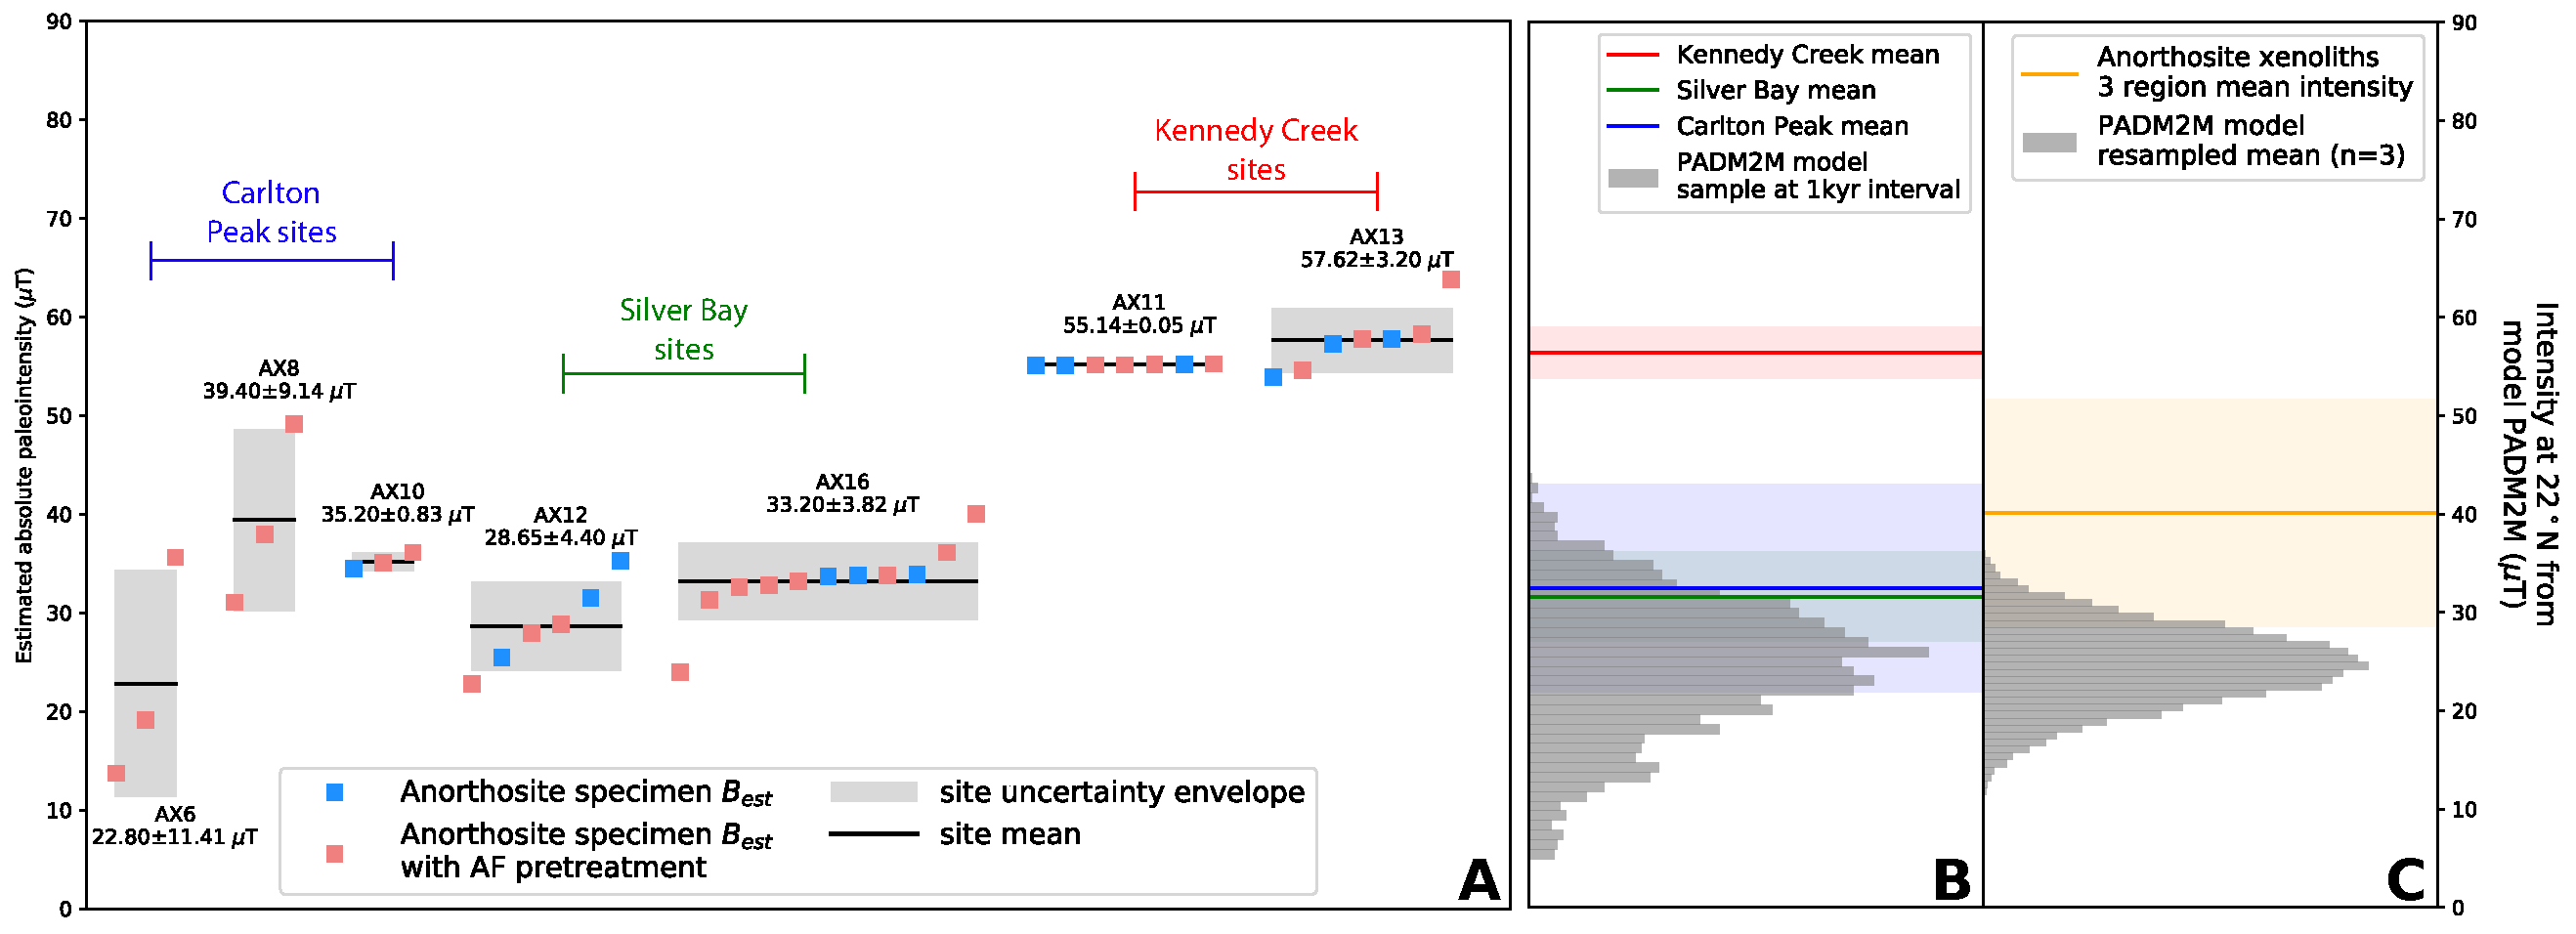
\includegraphics[width=\textwidth]{figure/Zhang2022/Paleointensity_plot_cooling_corrected.pdf}
\centering
\caption[Summary paleointensity results from the Beaver River anorthosite xenoliths]{\footnotesize{(A) Summary plot of individual specimen absolute paleointensity results (square symbols) and their averages and standard deviations at site level (black bars with grey one standard deviation uncertainty envelopes) where each `AX' site is an individual anorthosite xenolith within the Beaver River diabase. All results are corrected for cooling rate bias with a factor of 0.75. The sites with successful experiments come from 3 regions (Carlton Peak, Silver Bay, Kennedy Creek) which would have cooled at distinct times yielding similar estimates within each region with differences between regions. (B) Regional means calculated from the specimen-level data are compared to the distribution of intensities calculated from a paleomagnetic axial dipole moment model for the past 2 million years (PADM2M; \citealp{Ziegler2011a}) at the latitude corresponding to the paleolatitude of study region (22\textdegree N). (C) The mean of the 3 regional means is compared to means calculated from 3 random values drawn from the PADM2M model \citep{Ziegler2011a}. The distribution represents a total of 10,000 iterations of taking 3 random draws and calculating the mean. These comparisons highlight that these anorthosites' paleointensity values are strong in relation to the geomagnetic field over the past 2 million years. All shaded regions in (B) and (C) represent one standard deviation uncertainties.}}
\label{fig:PINT_cooling_corrected}
\end{figure*}

In addition to estimating paleointensity values by introducing a set of selection criteria to filter our experiment results, we applied an independent statistical method from \cite{Cych2021a} to all experimental data regardless of their NRM/TRM plot statistics to make a bias-corrected estimation of paleointensity (BiCEP). This Bayesian probabilistic method is based on the assumption that paleointensity estimates from specimens that come from a same cooling unit are distributed around a true paleointensity value with the various deflections being expressed as the curvature parameter of the NRM/TRM plot \citep{Paterson2011a}. The posterior paleointensity distributions from these sites with high-quality specimen-level data are in agreement with the site-level averages developed using the selection criteria approach (Fig. \ref{fig:PINT_cooling_corrected}; Fig. \ref{fig:PINT_BiCEP}). Overall, the high-quality results from the anorthosite xenoliths of the Beaver River diabase indicate that the anorthosite xenoliths record a high geomagnetic field ca. 1092 Ma. 

\subsection*{Rock magnetism}
\subsubsection*{Coercivity}
Additional rock magnetic data indicate that those anorthosite specimens which pass the paleointensity selection criteria contain dominant magnetic remanence carriers with magnetic properties similar to stoichiometric, non-interacting, single domain magnetite, whereas anorthosite samples that failed the paleointensity result selection along with all diabase samples have more pronounced populations of non-ideal carriers. Magnetic property measurement system (MPMS) data show that both the diabase and anorthosite contain (titano)magnetite as evidenced by the presence of the Verwey transition (Fig. \ref{fig:MPMS}; \citealp{Verwey1939a, Feinberg2015a}). Anorthosite specimens from sites that yield successful paleointensity results have Verwey transition temperatures near 120 K as expected for stochiometric magnetite with minimal Ti contents \citep{Ozdemir1993a}. However, diabase and anorthosite specimens that did not pass our paleointensity selection typically have Verwey transitions that are suppressed toward lower temperatures (Fig. \ref{fig:MPMS}), indicating that their magnetic grains either have relatively higher Ti content or have been partially oxidized \citep{Ozdemir1993a}. Another difference is that samples which pass paleointensity selection have distinctly higher average median destructive field values than other anorthosite and diabase specimens (Fig. \ref{fig:coercivity}). Single-component fits for coercivity spectra \citep{Maxbauer2016a} show that anorthosites having successful paleointensity results can contain magnetic grain populations that have higher coercivities. For these successful samples, median destructive (MDF) field values associated with back-field demagnetization experiments range from 44 to 144 mT with a median of 53 mT (Fig. \ref{fig:coercivity}). In contrast, other anorthosite and diabase specimens tend to have lower peak coercivities (MDF range of 18-35 mT with a median of 22 mT; Fig. \ref{fig:coercivity}). This result is consistent with an interpretation that magnetic grain populations with more multidomain-like behavior are responsible for the non-ideal paleointensity behaviors during experiments of such specimens \citep{Xu2004a}.

\begin{figure}
\noindent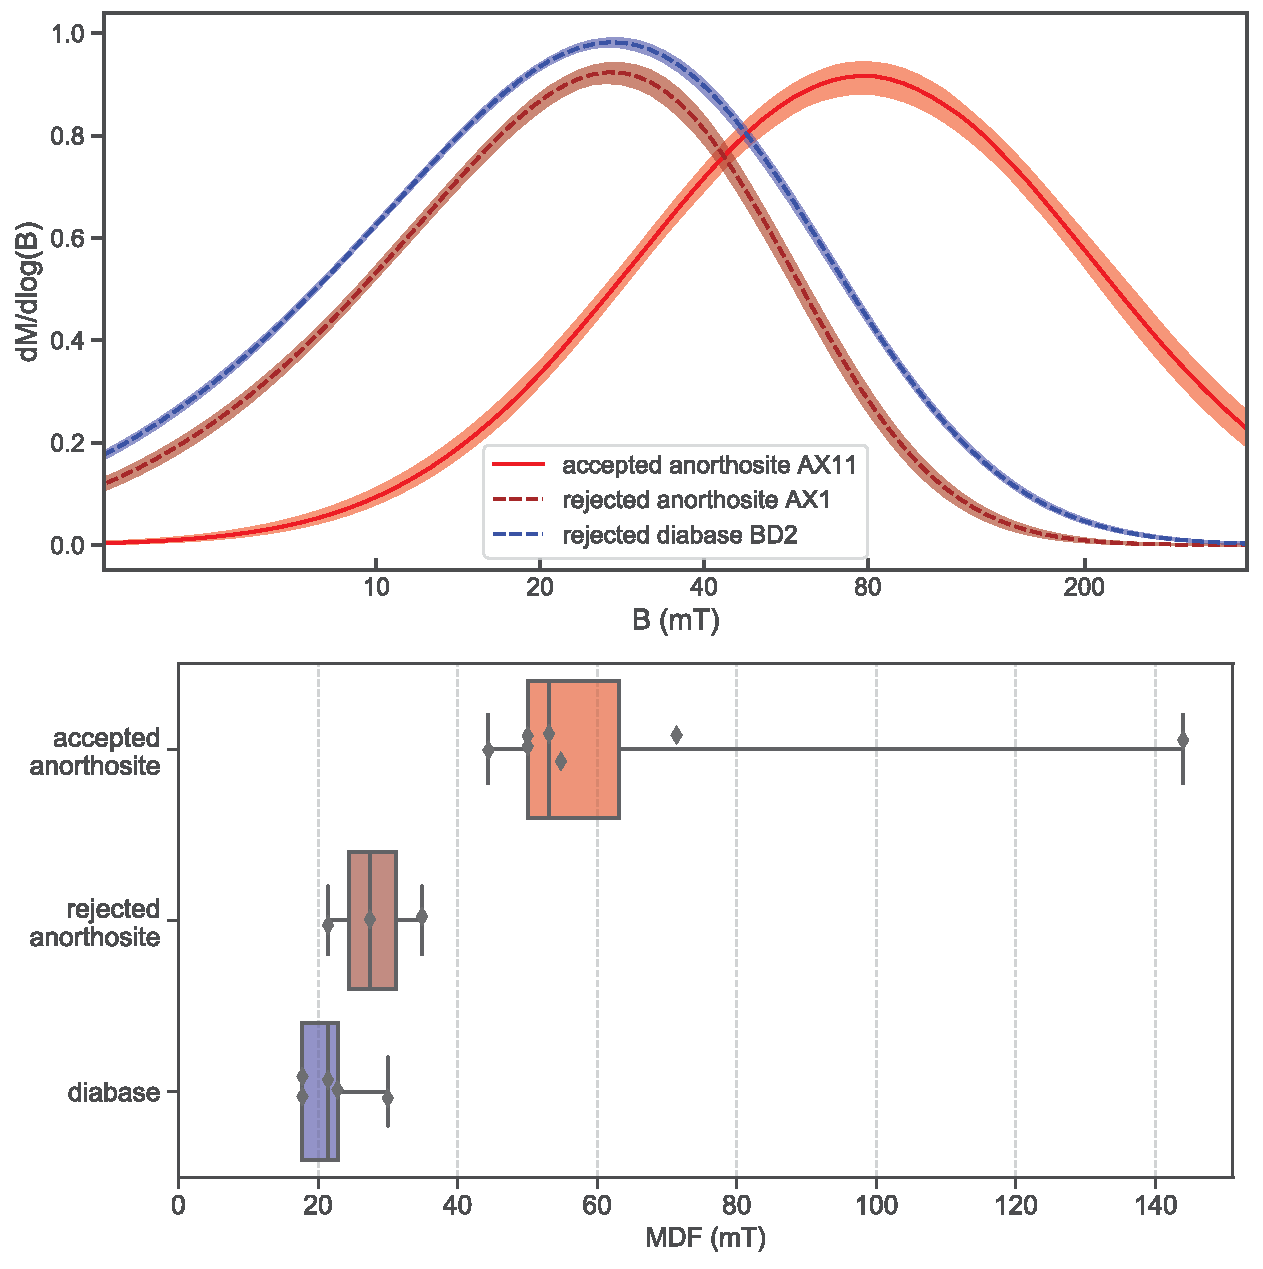
\includegraphics[width=0.58\textwidth]{figure/Zhang2022/coercivity.pdf}
\centering
\caption[Beaver River anorthosite xenoliths coercivity spectra and median destructive field (MDF) values associated with back-field demagnetization]{\footnotesize{Top: Example coercivity spectra of anorthosite and diabase chips from sites that pass or fail our paleointensity selection criteria. Bottom: Box plots of median destructive field (MDF) values associated with back-field demagnetization for all anorthosite and diabase specimens with single-component coercivity unmixing results. Bars in the boxes show median values and the whiskers show the minimum and the maximum value of the datasets. Both plots show that anorthosite specimens that pass paleointensity selection criteria have higher coercivities consistent with a higher portion of single-domain-like magnetite grains than the other anorthosite specimens and the diabase.}}
\label{fig:coercivity}
\end{figure}

\subsubsection*{Bulk TRM anisotropy}
Significant remanence anisotropy has been documented to exist within certain anorthositic rocks that formed in layered intrusive complexes \citep{Selkin2000a, Feinberg2006a}. Strong remanence anisotropy associated with the igneous foliation developed within anorthosite from the Stillwater Complex has been shown to cause significant overestimation or underestimation of paleointensity values depending on the relative orientations between the fabrics and an applied magnetic field \citep{Selkin2000a}. To assess whether our paleointensity estimates are biased by bulk remanence anisotropy, we calculated the gamma statistic, which is the angular difference between the last pTRM step of paleointensity experiment and the applied field direction. The results show that the anorthosite specimens used in our paleointensity experiment have low gamma values ranging from 0.9\textdegree$\;$ to 11.9\textdegree, with a median value of 4.2\textdegree$\;$(Table \ref{tab:PINT_result}). Because these anorthosite specimens were oriented at various directions with respect to the outcrops, the angles between the applied lab field direction during paleointensity experiments with respect to any fabrics within the anorthosite specimens are expected to cover a wide range of angles. These gamma values of the anorthosite xenolith bulk specimens are similar to those of the Midcontinent Rift volcanics studied by \cite{Sprain2018a}. Therefore, the bulk Beaver River anorthosite xenoliths do not have significant remanence anisotropy. Paleodirectional data from our anorthosite xenoliths indicate that they have minimal remanence anisotropy as their site mean directions closely match those of the Beaver River diabase hosts without deviating due to a fabric \citep{Zhang2021b}. These bulk results are consistent with the data from the grain-scale magnetic anisotropy experiments that also show minimal remenance anisotropy (Fig. \ref{fig:Petro_QDM}E, G). 

\subsection*{Considering secular variation and cooling rate}
To best characterize the geomagnetic axial dipole field intensity during a certain time period, a paleointensity dataset should cover a sufficient amount of time such that paleosecular variations of the geomagnetic field are averaged. Thermal modeling results from \citealp{Zhang2021b} indicate that the Beaver River anorthosite xenoliths were heated to tholeiitic magma temperature ($\sim$1100\textdegree C)---lower than the melting temperature of the anorthosite plagioclase (given its composition of 70\% anorthite; \citealp{Morrison1983a, Doyle2016a}) and acquired thermal remanent magnetization during cooling with their diabase host on a time scale of a few thousand years, partially averaging secular variation within single sites. Another consequence of the anorthosite xenoliths having slowly cooled in the interior of thick diabase intrusions is that slow cooling rates can bias paleointensity estimates toward higher values \citep{Halgedahl1980a}. Large differences in cooling rates between acquisition of an NRM in nature versus a TRM in the lab can result in overestimated paleointensities for single domain grains \citep{Dodson1980a, Halgedahl1980a, Nagy2021a}. From the thermal history model of \cite{Zhang2021b}, we can estimate the duration over which the diabase and anorthosite cooled from the Curie temperature of magnetite ($\sim$580\textdegree C) to the time when they blocked in the majority of their characteristic natural remanence magnetization ($\sim$500\textdegree  C; Fig. \ref{fig:IZZI_examples}; \citealp{Zhang2021b}). We find the cooling time to $\sim$500\textdegree C to be $\sim$1.5 kyr, which corresponds to a cooling rate of $\sim1.7\times10^{-9}$ $^\circ$C s$^{-1}$. In contrast, the lab cooling rate is much faster through the same temperature interval with an estimated cooling rate of $\sim1.3\times10^{-1}$ $^\circ$C s$^{-1}$. The significant cooling rate difference leads to a predicted $\sim$33\% overestimate of true ancient field following the model of \cite{Halgedahl1980a} (Fig. \ref{fig:SI_PINT_cooling_corrected}). This estimate on cooling rate effect is similar to the value of $\sim$30\% overestimate derived from the model of \cite{Nagy2021a}. We therefore correct our paleointensity results by a factor of 0.75. Remanence held by vortex state (pseudo-single domain) and multidomain grains is not as biased by cooling rate \citep{Biggin2013a}. The potential for some remanence to be held by these grains, as suggested by slightly zigzagging Arai plots (Fig. \ref{fig:IZZI_examples}), could mean that this factor is an over-correction and true paleointensity values could be slightly higher than those reported here. The cooling rate-corrected specimen paleointensity estimates together with specimen- and site-level means are shown in Fig. \ref{fig:PINT_cooling_corrected}.

Anorthosite xenoliths have paleointensity results that are consistent within small regions, but vary between regions. Anorthosite AX12 (28.65 $\pm$ 4.40 $\mu$T) and AX16 (33.20 $\pm$ 3.82 $\mu$T) in the Silver Bay area were emplaced $\sim$450 meters apart and have indistinguishable paleointensity estimates (Figs. \ref{fig:Chap_PINT_Geologic_map} and \ref{fig:PINT_cooling_corrected}). $\sim$10 km to the north, anorthosite xenoliths AX11 (55.14 $\pm$ 0.05 $\mu$T) and AX13 (57.62 $\pm$ 3.20 $\mu$T) in the Kennedy Creek area were also emplaced closely ($\sim$125 meters apart) and yield similar values to one another, but distinct paleointensity estimates from those of AX12 and AX16 (Figs. \ref{fig:Chap_PINT_Geologic_map} and \ref{fig:PINT_cooling_corrected}). $\sim$30 km further to the north in the Carlton Peak region, AX6 (22.80 $\pm$ 11.41 $\mu$T), AX8 (39.40 $\pm$ 9.14 $\mu$T), and AX10 (35.20 $\pm$ 0.83 $\mu$T) are anorthosite xenoliths within 10 meters of one another and also yield similar paleointensity estimates albeit with relatively large uncertainties (Fig. \ref{fig:PINT_cooling_corrected}). The anorthosites of the three distinct regions captured three different intervals of geomagnetic field intensities during the emplacement and cooling of the Beaver River diabase sills ca. 1092 Ma. To contextualize the high paleointensity values, we plot the regional mean values (Table \ref{tab:SI_PINT_regional_mean}) based on specimen-level paleointensity results together with calculated paleointensity values at 22\textdegree N latitude based on the PADM2M model of the time-varying geomagnetic field over the past 2 million years \citep{Ziegler2011a} in Figure \ref{fig:PINT_cooling_corrected}B. The locality-mean values of these three regions are plotted in Figure \ref{fig:PINT_cooling_corrected}C (and reported in Table \ref{tab:SI_PINT_regional_mean}) where we also present the distribution of means calculated from 3 random values taken from the PADM2M model for a total of 10000 iterations. In addition, we perform the same comparison with the existing paleointensity data for the Cenozoic Era (the last 66 million years) from the PINT database (filtered by Q$_{PI}\geq$3; Fig. \ref{fig:SI_Cenozoic_PINT}) given that the observational dataset could record more geomagnetic field excursions or regional high flux patches. The anorthosite xenoliths three region-mean intensity is higher than all values from the resample results of the PADM2M model, and rival the top 3\% values of the resample averages from the Cenozoic data (Fig. \ref{fig:SI_Cenozoic_PINT}). This comparison supports that the anorthosite xenoliths record an exceptionally strong geomagnetic field ca. 1092 Ma.

\begin{figure*}[h!]
\noindent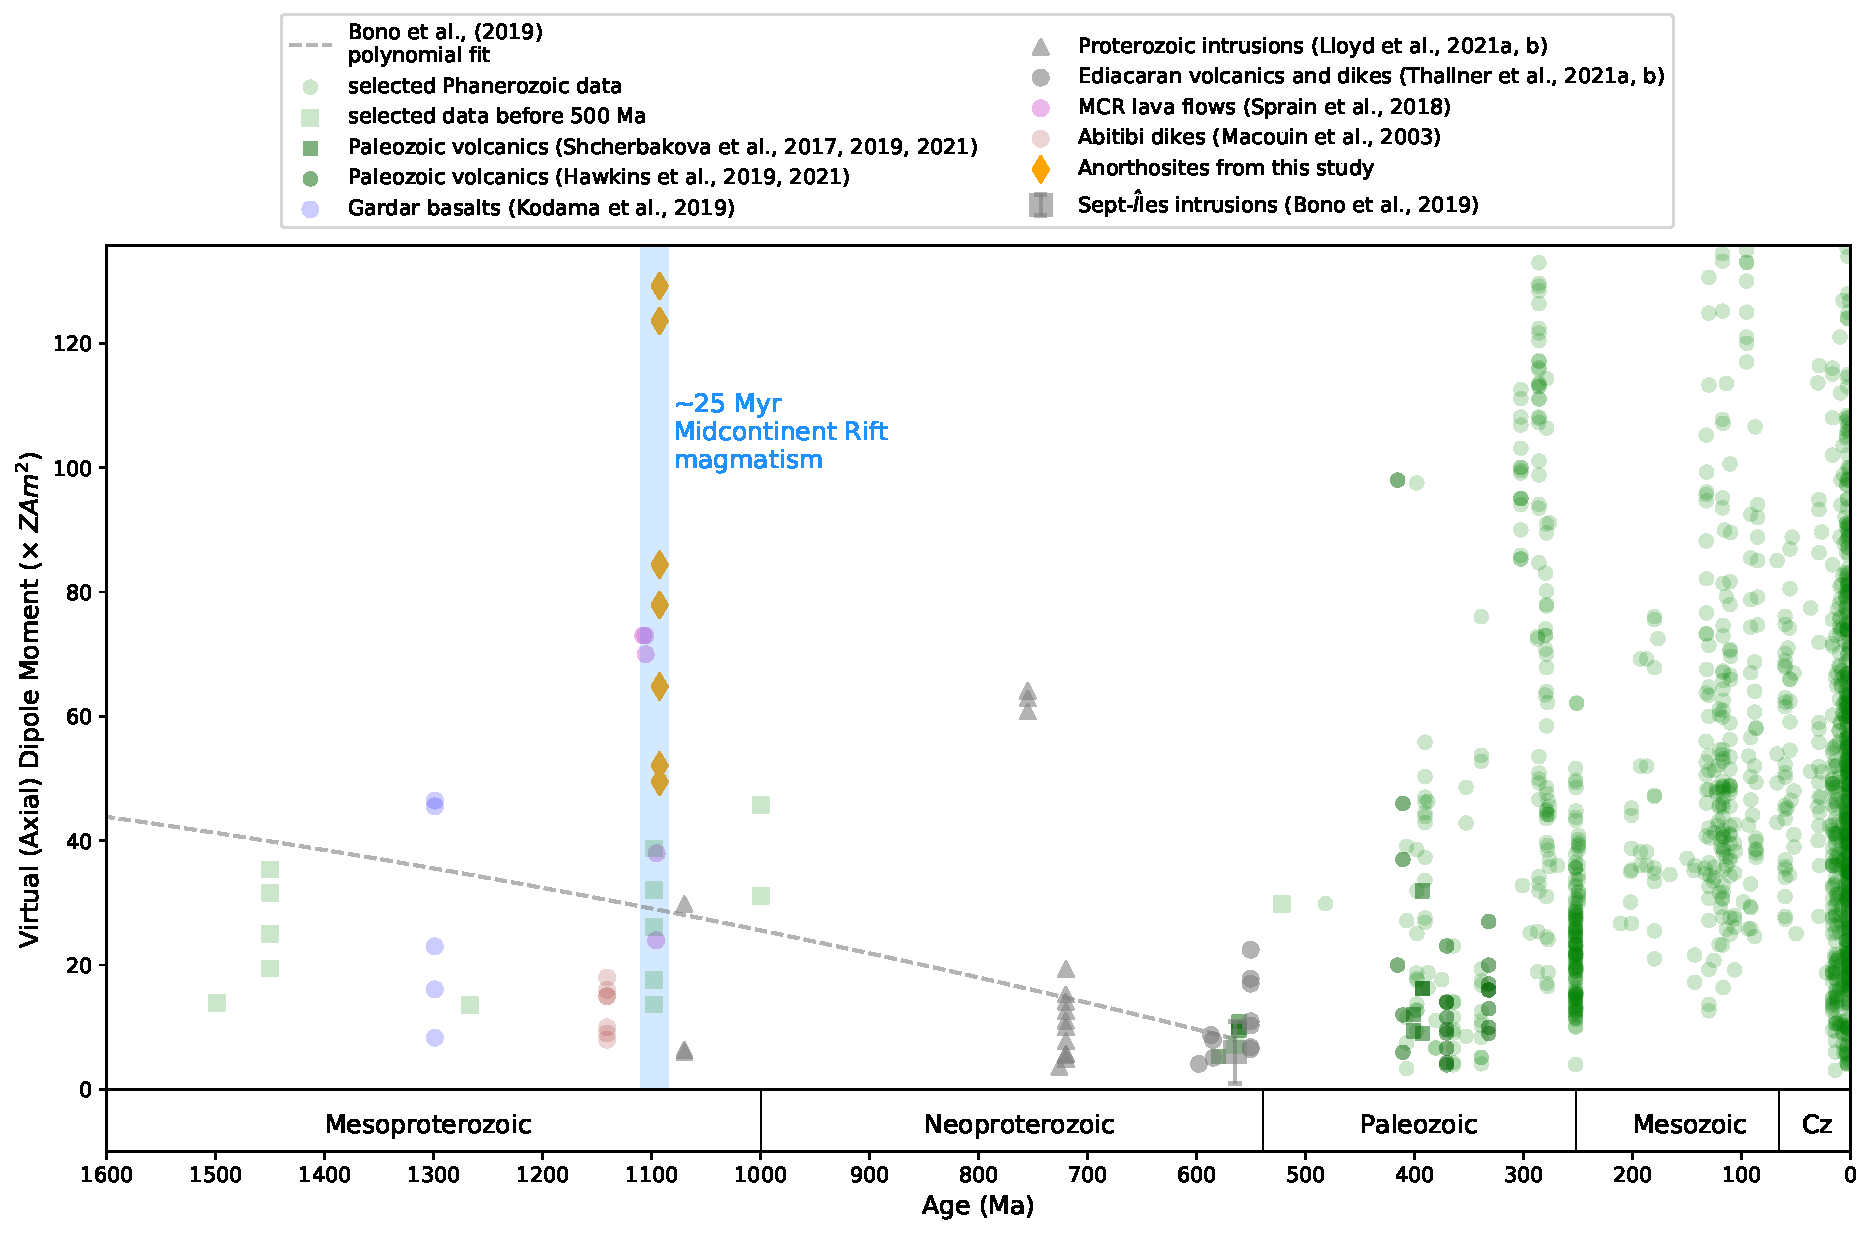
\includegraphics[width=\textwidth]{figure/Zhang2022/PINT_compilation.pdf}
\centering
\caption[Compilation of geomagnetic virtual (axial) dipole moment estimates through Earth's history]{\footnotesize{Compilation of calculated virtual (axial) dipole moment values from the PINT database (PINT v8.0.0; \url{http://www.pintdb.org/}; \citealp{Bono2022a}), including all Phanerozoic VDM and VADM records with Q$_{PI}$ values $>$3 and additional Neoproterozoic data from refs. \cite{Lloyd2021a, Lloyd2021b, Thallner2021b, Thallner2021a}. Paleointensity estimates from refs. \cite{Pesonen1983a} and \cite{Kulakov2013a} are not included in the compilation due to the specimen-level double-slope behavior as discussed in the text. Overall, the anorthosite xenoliths from this study record a high Mesoproterozoic field exceeding the value projected by the second order polynomial curve from \cite{Bono2019a} which is based on an interpretation of there being a monotonic decay of the geodynamo through the Proterozoic. The highest site-mean virtual dipole moment of the anorthosites would rank in the top 2$\%$ of those in the database for the Cenozoic Era (the last 66 million years) when there was unequivocally a crystallizing inner core. The y-axis maximum is set at the 99th percentile of the compiled Cenozoic paleointensity data.}}
\label{fig:PINT_compilation}
\end{figure*}

\section{Discussion}

The crystallization of the solid inner core is an important event in the long-term evolution of Earth's core and in sustaining the geodynamo \citep{Buffett2000a}. The age of the inner core in thermal evolution models relies on estimates for the thermal conductivity of iron alloys at the temperatures and pressures of the core \citep{Ohta2021a}. Prior to studies of the last 10 years, an accepted value of $\sim$30 W m$^{-1}$ K$^{-1}$ for this thermal conductivity constrained the timing of inner core nucleation to be during the first half of Earth's history \citep{Stacey2007a, Konopkova2016a}. Subsequently, experimental data and \textit{ab intio} simulations were interpreted to imply higher thermal conductivity values \citep{Pozzo2012a, Ohta2016a} which in turn implied a younger age for the inner core ($<$700 Ma; \citealp{Labrosse2015a}). However, other experimental studies continue to indicate lower thermal conductivity values consistent with prior estimates \citep{Konopkova2016a, Hsieh2020a} with no consensus yet emerging \citep{Williams2018a, Ohta2021a}. These experiments are challenging to conduct and interpret given complexities such as constraining the sample thickness under high pressure and temperature conditions, the validity of applying the Wiedemann-Franz law to extrapolate thermal conductivity values based on electrical resistivity measurements \citep{Ohta2016a}, and propagating uncertainties from free parameters used in finite element modeling of direct thermal conduction experiments \citep{Konopkova2016a}. Further experiments and theory are needed to explain these contrasting results which at present leave open very different trajectories for Earth's thermal evolution. As a result, the age of the inner core is relatively unconstrained from a theoretical perspective. 

The other data type that can provide insight into the long-term history of the core's thermal regime and geodynamo is paleomagnetic data---both paleodirectional data that indicate the presence of a geomagnetic field and paleointensity data that constrain the field's strength. Inner core nucleation would have increased the power to the geodynamo which has the potential to manifest as an increase in Earth's surface field \citep{Davies2021a}. An approach combining dynamo simulations and theoretical scaling relationships has predicted that progressive decay of the field's dipole moment would be followed by a rapid increase in geomagnetic field intensity soon after the onset of inner core nucleation such that a minimum in dipole moment would occur just before inner core nucleation \citep{Davies2021a}. Other scenarios are possible, however, such as the model-based prediction that while power increases associated with inner core nucleation strengthen Earth's internal magnetic field, that the dynamo becomes more deeply seated in the core diminishes the increase in magnetic field strength at Earth's surface \citep{Aubert2009a, Landeau2017a}. Such a scenario where the dynamo shifts to a greater depth associated with inner core nucleation led \citealp{Aubert2009a} to conclude that the increase in power to the dynamo would be difficult to detect with paleointensity data. Ultimately, further observational paleomagnetic records are key as they hold the potential for testing different model predictions and identifying transitions in ancient field strength \citep{Biggin2015a, Bono2019a}.

It has been proposed that Proterozoic paleointensity data are consistent with a progressive monotonic decay leading to a minimum ca. 565 Ma in the Ediacaran Period (Fig. \ref{fig:PINT_compilation}; \citealp{Bono2019a}). This interpretation was motivated by paleointensity estimates developed from the ca. 565 Ma Sept-$\hat{I}$les layered mafic intrusive complex of $\sim$7 ZAm$^2$ that are among the lowest values in the paleointensity database (Fig. \ref{fig:PINT_compilation}; \citealp{Bono2019a}). A decay in the lead-up to this time was argued to be consistent with an absence of an inner core and a dynamo to which progressively less power was available through secular cooling \citep{Bono2019a, Davies2021a}. This timing of inner core formation would favor a high core thermal conductivity \cite[e.g.][]{Ohta2016a}. Paleomagnetic directional excursions \citep{Halls2015a}, other weak paleointensity estimates \citep{Thallner2021b}, and frequent polarity reversals \citep{Kodama2021a} in rocks of similar age are interpreted to be consistent with numerical simulations \citep{Driscoll2016a} associated with a weak dipole field. 

The high paleointensity estimates from the 1.1 billion-year-old Midcontinent Rift rocks challenge the hypothesized monotonic decay of the geomagnetic field strength throughout the Proterozoic Era (Fig. \ref{fig:PINT_compilation}). The well-preserved ca. 1092 Ma anorthosite xenoliths of the Beaver River diabase record a strong geomagnetic field in the late Mesoproterozoic that exceeds the modern-day field strength for which crystallization of the inner core is a power source (Figs. \ref{fig:PINT_cooling_corrected} and \ref{fig:PINT_compilation}). Together with previous records obtained from the ca. 1106 Ma Osler Volcanics of the Midcontinent Rift \citep{Sprain2018a}, these data indicate that appreciable power to Earth's dynamo persisted through at least 14 Myr during the late Mesoproterozoic to maintain a strong surface field (Fig. \ref{fig:PINT_compilation}). In addition to these high geomagnetic fields recorded by Midcontinent Rift rocks, the ca. 755 Ma Mundine Well dikes \citep{Lloyd2021b} also require a stronger geomagnetic field in the Neoproterozoic than would be predicted by a progressive Proterozoic decline. Taken together, these results call into question whether the progressively decaying polynomial fit implemented by \cite{Bono2019a} is an accurate representation for the evolution of the Proterozoic geomagnetic field (Fig. \ref{fig:PINT_compilation}). 

The hypothesis that a weak Ediacaran geomagnetic field is a telltale sign of the lack of an inner core with core nucleation following shortly thereafter may predict that it is the most significant weak to strong field transition in the paleointensity record. However, Fig. \ref{fig:PINT_compilation} shows that transitions from low to high field intensities occurred before, during, and after the Ediacaran Period. In the Ediacaran record developed to date, there is a two-fold increase in Earth's virtual dipole moment when comparing estimates from the ca. 565 Ma Sept-$\hat{I}$les intrusions \citep{Bono2019a} to those from ca. 550 Ma volcanics of the Skinner Cove Formation (Fig. \ref{fig:PINT_compilation}; \citealp{Thallner2021a}). In the late Mesoproterozoic, there is at least a six-fold increase within a period of $\sim$35 Myr from a low average virtual dipole moment of $\sim$13 ZAm$^2$ recorded by the ca. 1140 Ma Abitibi dikes which yielded straight Arai plots \citep{Macouin2003a}, to a high moment of $\sim$70 ZAm$^2$ recorded by the ca. 1106 Ma Osler Volcanics, with even stronger values from ca. 1092 Ma by Beaver River anorthosite xenoliths that record virtual dipole moments up to $\sim$129 ZAm$^2$. While the ca. 1140 Abitibi dikes' paleointensity estimates are not as low as those of the ca. 565 Ma Sept-$\hat{I}$les intrusions, this virtual dipole moment increase in the Mesoproterozoic from the ca. 1140 Ma data to the ca. 1100 Ma data is the largest yet documented in the Precambrian on a 10s of millions of years timescale (Fig. \ref{fig:PINT_compilation}). The tempo and scale of this field intensity transition could match with model-based predictions associated with the onset of inner core nucleation \citep{Davies2021a}. This ca. 1.1 Ga timing would be broadly consistent with the ca. 1.3 Ga onset proposed by \cite{Biggin2015a} albeit later given the exclusion of previous overestimated paleointensity values from the ca. 1.3 Ga Gardar basalts that are superseded by data in \cite{Kodama2019a}. However, a model prediction of sustained strong field values following inner core nucleation is challenged by data from the ca. 1070 Ma Bangemall Sills which include a sill with a low virtual dipole moment of $\sim$6.4 ZAm$^2$ (Fig. \ref{fig:PINT_compilation};  \citealp{Lloyd2021b}). Following the Ediacaran, there are also low paleointensity estimates from Devonian rocks such as the ca. 370 Ma dikes and lavas of the Siberian Viluy Traps that give virtual dipole moment estimates of 4.3 to 14.9 ZAm$^2$ (Fig. \ref{fig:PINT_compilation}; \citealp{Hawkins2019a}). These low values as well as data from the ca. 414 Ma Strathmore lava flows \citep{Hawkins2021a}, the ca. 410-380 Ma lava flows of Siberia and the Kola Peninsula \citep{Shcherbakova2017a}, the ca. 408–393 Ma Buribay volcanics \citep{Shcherbakova2021a} and the ca. 332 Ma Kinghorn volcanics \citep{Hawkins2021a} have led to the proposal of this interval being the ``Mid-Paleozoic Dipole Low'' \citep{Hawkins2021a}. This ``Mid-Paleozoic Dipole Low'' is followed by high paleointensity values such that there is a six-fold increase from virtual dipole moments of $\sim$16 ZAm$^2$ ca. 332 Ma to $\sim$99 ZAm$^2$ ca. 308 Ma in the late Carboniferous (Fig. \ref{fig:PINT_compilation}; \citealp{Hawkins2021a}). 

Given that the multiple records of a weak field in the Proterozoic and Paleozoic cannot all be the minimum prior to the singular event of the onset of inner core nucleation, what processes could lead to a weak dipole at Earth's surface even in the presence of a crystallizing inner core? Numerical models have shown that the dipole moment is sensitive to both the magnitude and spatial pattern of heat flow across the core-mantle boundary when there are strong available power sources to the geodynamo \citep{Olson2007a, Olson2010a}. In such models, relatively low total heat flux across the core-mantle boundary can prevent the axial dipole from reversing whereas a high heat flux through the boundary can result in an increase in reversal frequency and decrease in dipole intensity. The ``Mid-Paleozoic Dipole Low'' has been hypothesized to be the result of such elevated core-mantle boundary heat flux conditions at a time when there was also available power from a crystallizing inner core \citep{Hawkins2019a}, thereby also explaining the observed low paleointensities which include values as weak as those of the ca. 565 Ma Sept-$\hat{I}$les intrusions (Fig. \ref{fig:PINT_compilation}; \citealp{Bono2019a}). Mantle convection can modulate core mantle boundary heat flow through changes in the structure of the deep mantle associated with upwelling plumes \citep{Larson1991a, Courtillot2007a} and subducted slabs \citep{Tan2002b, Biggin2012a, Hounslow2018a}. Strong evidence for differential plate tectonic motion extends back to ca. 2.2 Ga in the Paleoproterozoic \citep{Mitchell2014a, Swanson-Hysell2021b} and potentially back to ca. 3.2 Ga in the Archean \citep{Brenner2020a}. Plate tectonic modulations of core mantle boundary heat flow are therefore expected throughout the Proterozoic. Such changes may explain large variability in Proterozoic paleointensity values similar to those seen in the Phanerozoic \citep{Lloyd2021a} and may challenge our ability to detect the increase in surface geomagnetic field strength predicted to have happened at the onset of inner core crystallization. 

Overall, the high-fidelity paleointensity recorders of the Beaver River anorthosite xenoliths in the well-preserved Midcontinent Rift record strong field strengths 1.1 billion years ago. The highest site-level value of the virtual dipole moment would rank in the top 2$\%$ of those in the database for the Cenozoic Era when there was unequivocally a crystallizing inner core. These high surface field strengths necessitate that appreciable power was provided to the late Mesoproterozoic geodynamo. 

\section{Acknowledgements}

Project research was supported by NSF CAREER grant EAR-1847277 to N.L.S.-H., an Institute on Lake Superior Geology Student Research Fund grant to Y.Z., and an Institute for Rock Magnetism Visiting Student Fellowship to Y.Z. The Institute for Rock Magnetism is supported by the Instrumentation and Facilities program of the NSF Earth Science Division. Permits for fieldwork and sampling from the Minnesota Department of Natural Resources are gratefully acknowledged. We thank James Pierce and Blake Hodgin for their assistance in the field. We thank Jim Miller for providing us with the Duluth Complex anorthosite thin section. We thank Dario Bilardello, Peat Solheid, Mike Jackson, Josh Feinberg, and Bruce Moskowitz for their tremendous help with instrument operation, data interpretations, and research guidance at the IRM. Conversations with Bruce Buffett and Zachary Geballe informed our perspectives on the geodynamic and mineral physics literature. We thank Jon Hagstrum at USGS and two anonymous reviewers for their helpful comments on the manuscript.

\chapter[Tracking Rodinia into the Neoproterozoic: new paleomagnetic constraints from the Jacobsville Formation][Tracking Rodinia into the Neoproterozoic]{Tracking Rodinia into the Neoproterozoic: new paleomagnetic constraints from the Jacobsville Formation}

\let\thefootnote\relax\footnote{This chapter is published as a peer-reviewed manuscript: Zhang, Y., Hodgin, E.B., Mohr, M.T., Alemu, T.B., Pierce, J., Fuentes, A.J., Swanson-Hysell, N.L. (2024). Tracking Rodinia into the Neoproterozoic: new paleomagnetic constraints from the Jacobsville Formation. Tectonics. doi: \url{https://doi.org/10.1029/2023TC007866.}}

\section{Abstract}
The paleogeography of Laurentia throughout the Neoproterozoic is critical for reconstructing global paleogeography due to its central position in the supercontinent Rodinia. We develop a new paleomagnetic pole from red siltstones and fine-grained sandstones of the early Neoproterozoic Jacobsville Formation which is now constrained to be ca. 990 Ma in age. High-resolution thermal demagnetization experiments resolve detrital remanent magnetizations held by hematite. These directions were reoriented within siltstone intraclasts and pass intraformational conglomerate tests---giving confidence that the magnetization is detrital and primary. An inclination-corrected mean paleomagnetic pole position for the Jacobsville Formation indicates that Laurentia's motion slowed down significantly following the onset of the Grenvillian orogeny. Prior rapid plate motion associated with closure of the Unimos Ocean between 1110 and 1090 Ma transitioned to slow drift of Laurentia across the equator in the late Mesoproterozoic to early Neoproterozoic. We interpret the distinct position of this well-dated pole from those in the Grenville orogen that have been assigned a similar age to indicate that the ages of the poles associated with the Grenville Loop likely need to be revised to be younger due to prolonged exhumation. 

\section{Introduction}

The extensively studied paleomagnetic records of ca. 1109 to 1084 Ma volcanics and intrusions associated with the North American Midcontinent Rift provide crucial constraints on the paleogeography of Laurentia in the late Mesoproterozoic Era \citep{Halls1982a, Fairchild2017a, Swanson-Hysell2019a}. The resulting sequence of poles known as the Keweenawan Track is a central record for reconstructing the assembly of the ancient supercontinent Rodinia \citep{Evans2021b}. An advantage of intracratonic magmatic events, such as those preserved in the Midcontinent Rift, is that they lead to emplacement of igneous rocks that can readily retain primary thermal remanent magnetization (TRM) that can be confidently associated with the emplacement age of the unit. However, following the development of the Midcontinent Rift, there was a $\sim$300 Myr quiescence in known intracratonic magmatic activity in Laurentia that lasted until the emplacement of the ca. 775 Ma Gunbarrel large igneous province \citep{Harlan2003a, Mackinder2019a, Swanson-Hysell2021c}. The lack of Laurentian rocks with primary TRM in the early Neoproterozoic has led paleogeographic reconstructions to be reliant on magnetizations acquired by rocks that were metamorphosed during the ca. 1090 to 980 Ma Grenvillian orogeny \citep{Rivers2008a, Rivers2012a, Swanson-Hysell2023a}. However, rocks within the orogen acquired their magnetizations during exhumation after peak metamorphic conditions \citep{McWilliams1975a}. As a result, the timing of remanence acquisition needs to be constrained through the more difficult task of dating cooling associated with exhumation. This gap in well-dated paleomagnetic poles for Laurentia in the late Mesoproterozoic to mid-Neoproterozoic contributes to uncertainty in paleogeography at that time including the configuration of the supercontinent Rodinia.

\begin{figure*}[h!]
\centering
\includegraphics[width=\textwidth]{figure/Zhang2024a/Geologic_map.pdf}
\caption[Overview map of the Midcontinent Rift and the geologic map of the Jacobsville Formation and associated units]{(A) Regional map showing the extent of the Midcontinent Rift and the location of the Grenville Front relative to the study area. The inset green box shows the extent of panel B. (B) Geologic map of northern Michigan and Wisconsin showing Midcontinent Rift igneous and sedimentary rocks, sedimentary rocks of the Jacobsville Formation and Bayfield Group, other older Paleoproterozoic and Archean rocks, and major post-rift thrust faults. The location of the Jacobsville stratigraphic sections in this study are shown with green diamonds. Map modified from \cite{Nicholson2004a}.}
\label{fig:Chap_Jacobsville_Geologic_map}
\end{figure*}

Paleomagnetic poles can also be developed from sedimentary rocks deposited in basins. Sedimentary rocks of the Oronto Group deposited during post-rift thermal subsidence following the bulk of Midcontinent Rift magmatic activity provide paleomagnetic poles that extend the Keweenawan Track to ca. 1070 Ma \citep{Henry1977a, Slotznick2023a}. While there are some contemporaneous basins in northern Laurentia \citep{Greenman2021a}, there is minimal basin development within Laurentia following the Grenvillian orogeny until the Rodinia supercontinent began to rift apart ca. 770 Ma \citep{Macdonald2023a}. 

One rare preservation of an early Neoproterozoic sedimentary succession in Laurentia's interior is the Jacobsville Formation (Fig. \ref{fig:Chap_Jacobsville_Geologic_map}; \citealp{Hamblin1958a, Hodgin2022a, DeGraff2022a}). U-Pb detrital zircon dates developed through chemical abrasion–isotope dilution–thermal ionization mass spectrometry (CA-ID-TIMS) of 1003.21 $\pm$ 2.23 Ma and 992.51 $\pm$ 0.64 Ma (2$\sigma$ analytical uncertainty) constrain the maximum deposition age of the Jacobsville Formation \citep{Hodgin2022a}. A 985.5 $\pm$ 35.8 Ma (2$\sigma$ analytical uncertainty) U-Pb date from calcite veins within the Keweenaw fault provides a minimum age constraint on Jacobsville deposition, as the Jacobsville Formation is folded in the footwall against Midcontinent rift volcanics in the hanging wall. Together, these dates bracket the depositional age of the Jacobsville Formation and constrain it to be ca. 990 Ma \citep{Hodgin2022a}. These results support the interpretation that the formation was deposited within a syn-orogenic basin during the Rigolet phase of the Grenvillian orogen and was then deformed during the same orogenic phase.

The Jacobsville Formation contains abundant hematite-bearing sandstone and siltstone which have the potential to record a key pole in Laurentia's apparent polar wander path (APWP) \citep{Dubois1962a, Roy1978a}. \cite{Roy1978a} conducted a paleomagnetic study that developed a pole which has been used in paleogeographic syntheses where it has been assigned variable ages including an age of ca. 1020 Ma based on APWP extrapolation \cite[e.g.][]{Li2008a}. However, the uncertainty in the age of the magnetization combined with a lack of field tests, and no application of inclination correction have resulted in the pole not being included in recent curated compilations \cite[e.g.][]{Evans2021a}. Obtaining high-quality paleomagnetic data, including robust field tests, motivates the development of new data from the Jacobsville Formation. 

In this study, we investigate five stratigraphic sections of the Jacobsville Formation on and near the Keweenaw Peninsula, Michigan, USA (Figs. \ref{fig:Chap_Jacobsville_Geologic_map} and \ref{fig:strat_column}). These sections were chosen given the abundance of fine-grained siliciclastic lithologies where magnetization can be constrained through intraclast conglomerate field tests. Additionally, they are within the continuous bedrock belt from which chronostratigraphic constraints have been developed. In contrast to fluvial sandstones in other exposures such as in the eastern Lake Superior region near Sault Ste. Marie, the maximum and minimum depositional ages of these sections can be more confidently constrained. 

Within sampled lithologies, high-resolution thermal demagnetization isolates primary detrital remanent magnetization (DRM) from secondary chemical remanent magnetization (CRM). This interpretation is supported by the DRM directions passing intraformational conglomerate tests on siltstone intraclasts that were ripped-up and remobilized within the fluvial depositional environment. A paleomagnetic fold test further constrains the timing of DRM acquisition to predate the folding of the Jacobsville Formation in the footwall of the Keweenaw Fault soon after deposition. With these data, we develop a new inclination-corrected paleomagnetic pole for the Jacobsville Formation based on a large number of samples that gives new constraints on the paleogeographic position of Laurentia in the earliest Neoproterozoic.

\section{Geologic setting}

The ca. 1109 Ma to 1084 Ma North American Midcontinent Rift is a major intracontinental rift system that extends over 2000 km through the Laurentia craton (Fig. \ref{fig:Chap_Jacobsville_Geologic_map}). Following the end of active extension in the rift, thermal subsidence resulted in the accumulation of $>$4 km of ca. 1085-1050 Ma Oronto Group strata that are both intercalated with the youngest volcanics and deposited atop them (Fig. \ref{fig:Chap_Jacobsville_Geologic_map}; \citealp{Daniels1982a, Cannon1989a}). Subsequently, the rift was inverted as contraction associated with the ca. 1090-980 Ma Grenvillian Orogeny on the eastern margin of Laurentia (Fig. \ref{fig:Chap_Jacobsville_Geologic_map}) propagated into Laurentia's interior \citep{Cannon1993a, Cannon1994a, Hodgin2022a, Swanson-Hysell2023a}. 

During rift inversion, Midcontinent Rift volcanic and sedimentary rocks were uplifted along with Paleoproterozoic and Archean lithologies via thrust faults such as the Marenisco fault, forming the crustal-scale Montreal River monocline (Fig. \ref{fig:Chap_Jacobsville_Geologic_map}; \cite{Cannon1993a}). Rb-Sr biotite thermochronology data of \cite{Cannon1993a} show Archean lithologies within the Montreal River monocline to have been exhumed to mid to shallow crustal temperatures ($\sim$270\textdegree C) by ca. 1050 Ma. The Jacobsville Formation overlies an angular unconformity that developed on lithologies that were exhumed through this earlier episode of contractional deformation associated with Grenvillian orogenesis (Fig. \ref{fig:Chap_Jacobsville_Geologic_map}; \citealp{Hamblin1958a, Cannon1993a, Kalliokoski1982a}). Conglomeratic facies occur in the basal Jacobsville Formation, with clasts derived from locally uplifted basement lithologies \citep{Irving1885a, Hamblin1958a, Kalliokoski1982a}.

Bedding planes in the Jacobsville Formation typically have shallow dips. The exception to these near-horizontal orientations is proximal to reverse faults such as the Keweenaw fault (Fig. \ref{fig:Chap_Jacobsville_Geologic_map}) where the Jacobsville Formation was occasionally deformed into monoclinal drag folds resulting in steeply tilted to overturned beds (Fig. \ref{fig:Chap_Jacobsville_Geologic_map}; \citealp{Irving1885a, Cannon2001a}). Recent mapping of the Jacobsville Formation also found that it sometimes onlaps the Midcontinent Rift volcanics within or adjacent to en echelon fault branches of the Keweenaw fault system near the northern end of the Keweenaw Peninsula \citep{Tyrrell2019a, Mueller2021a}. These observations are consistent with the interpretation that there was deposition of Jacobsville Formation sediments during faulting.

\subsection{Overview of Jacobsville sedimentology and stratigraphy}

The Jacobsville Formation is a fluvial succession of feldspathic and quartzose conglomerates, sandstones, siltstones, and shales devoid of lava flows or cross-cutting igneous dikes although internal clastic dikes are present \citep{Hamblin1958a}. Sandstones of the Jacobsville Formation are more quartz-rich with generally fewer lithic fragments than sandstones of the Oronto Group such that they can typically be classified as subarkose to quartz arenites (Fig. \ref{fig:Field_photo}; \citealp{Hamblin1958a, Ojakangas2002a}). While much of the Jacobsville Formation is dominated by sandstone channel deposits, there are clay-rich siltstones that formed in overbank settings that are a major focus of this study.

\begin{figure*}[h!]
\centering
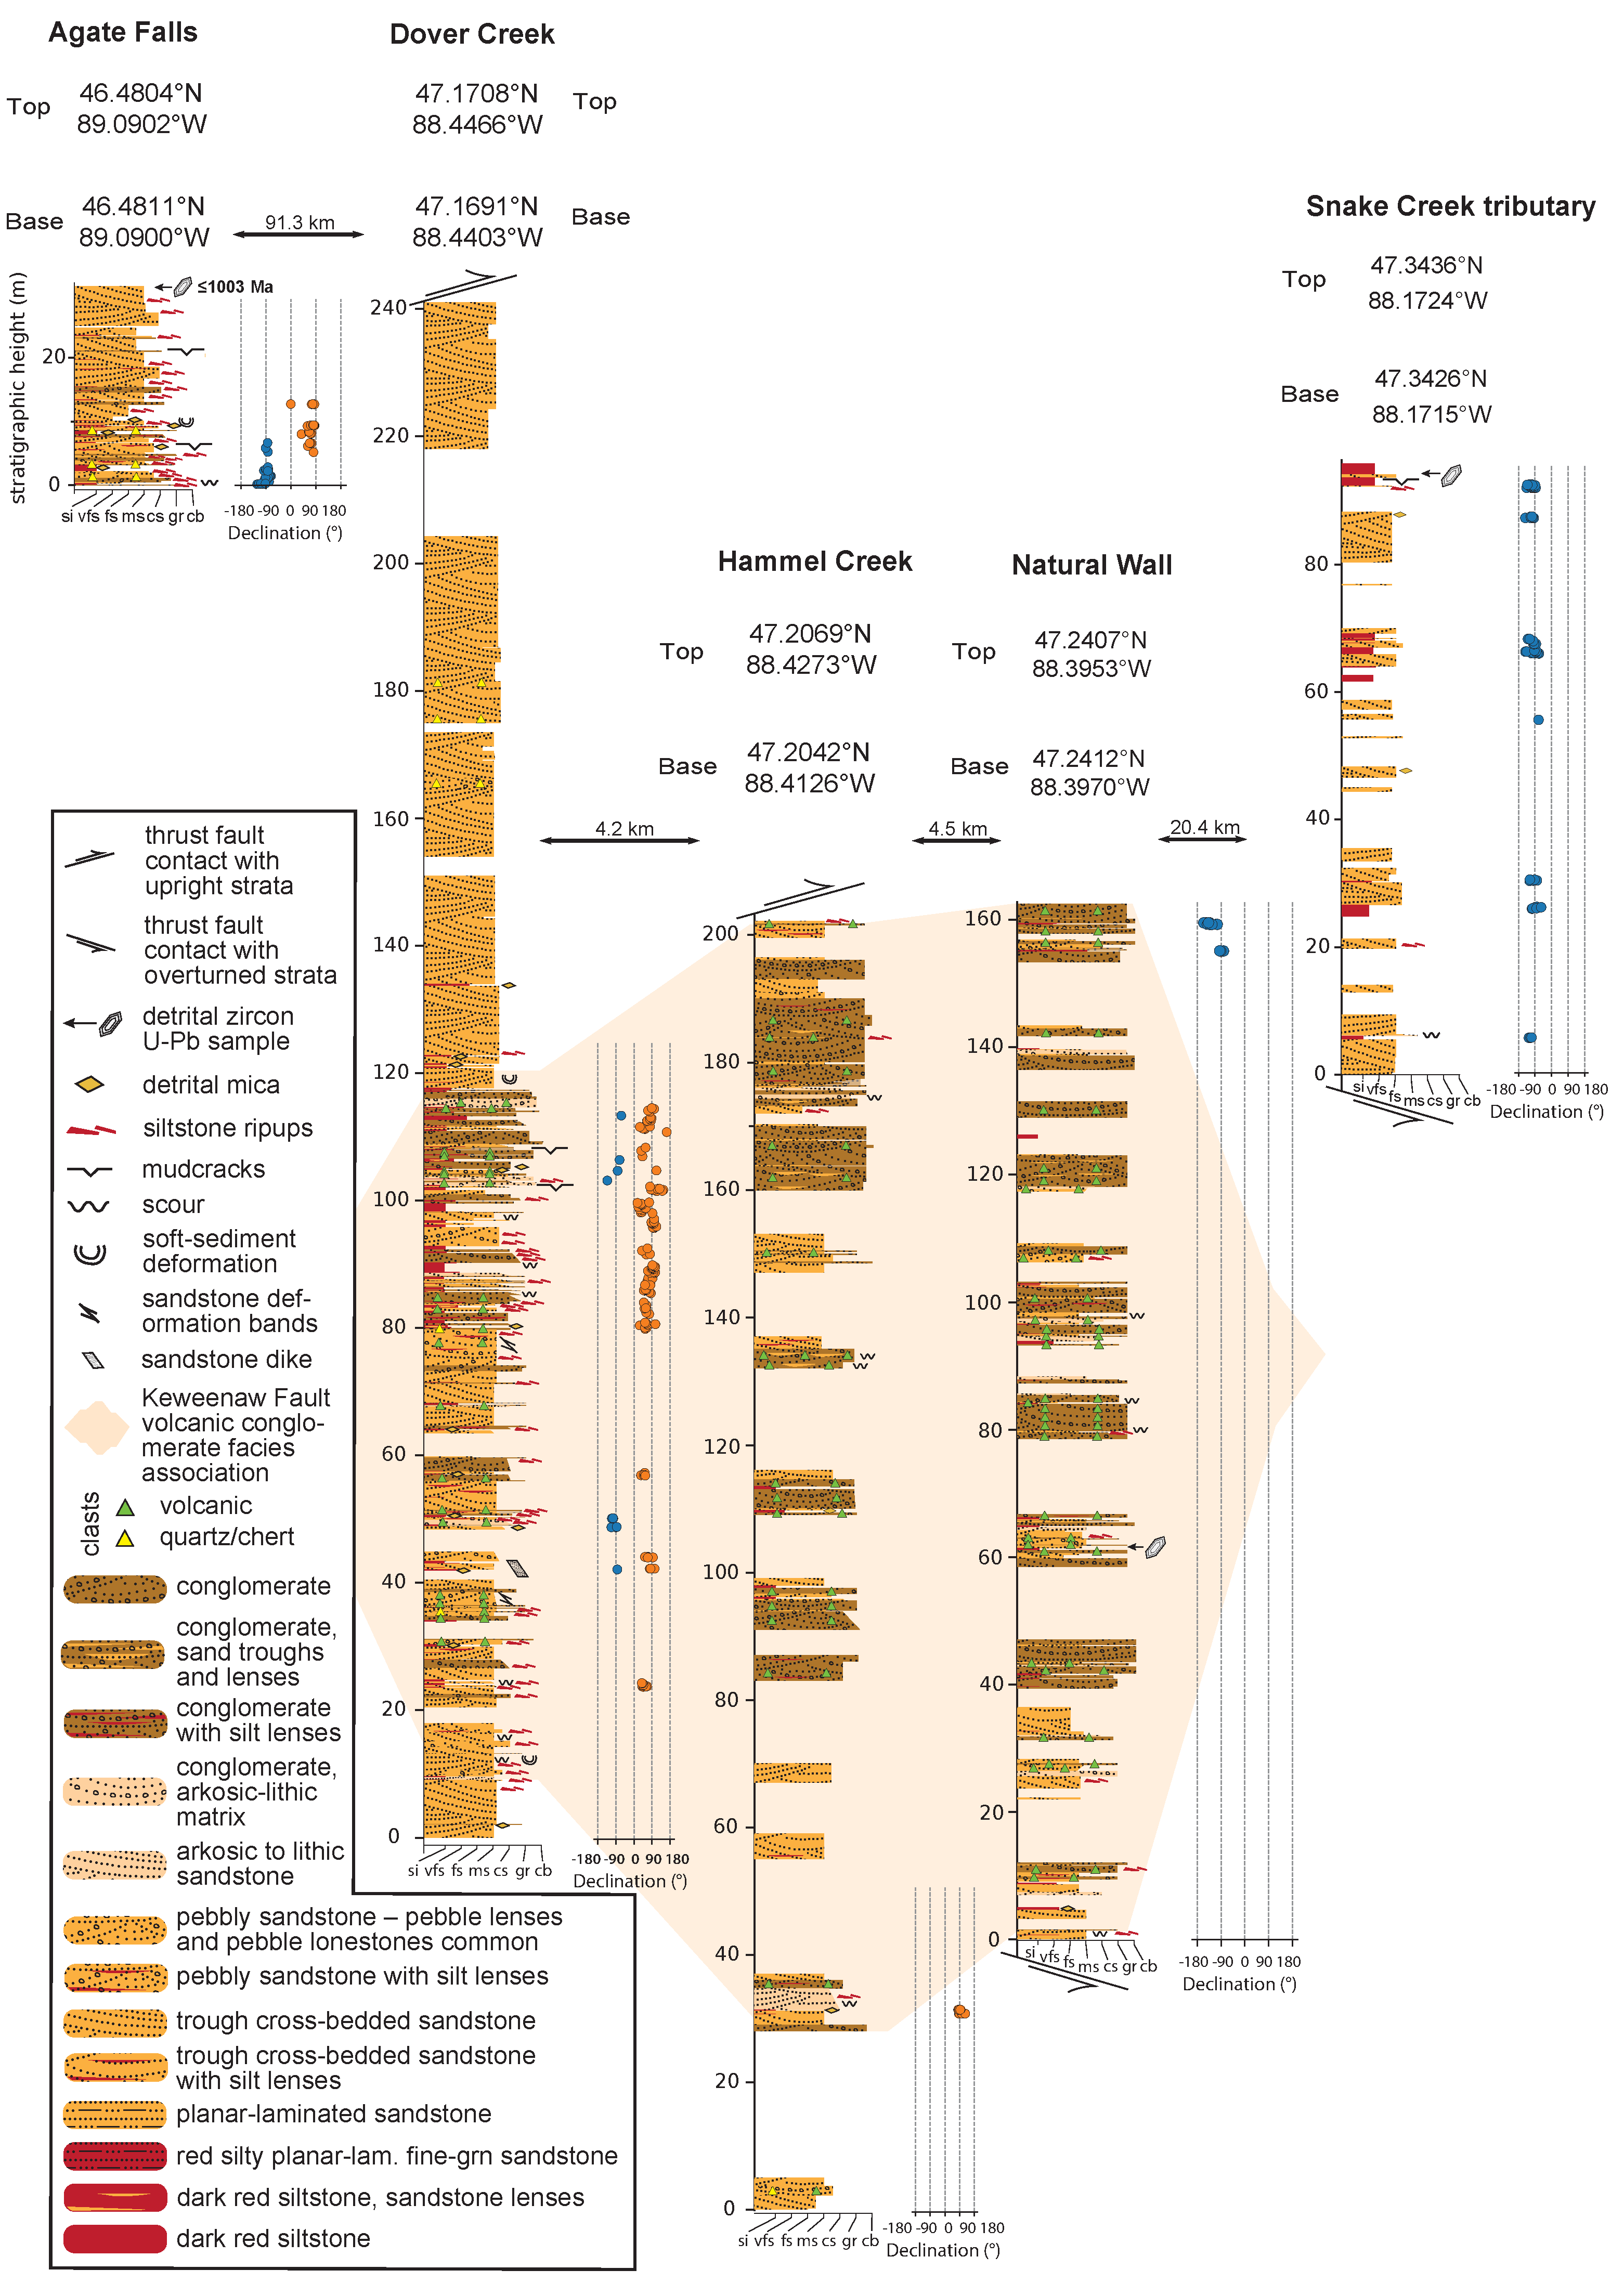
\includegraphics[width=0.6\textwidth]{figure/Zhang2024a/Jacobsville_Sections_v6.pdf}
\caption[Lithostratigraphy and magnetostratigraphy for studied sections of the Jacobsville Formation]{\footnotesize Lithostratigraphy and magnetostratigraphy for studied sections of the Jacobsville Formation in northern Michigan, USA. GPS locations for the base and top of the sections are noted. Paleomagnetic sampling focused on the dark red siltstone to fine-grained sandstone lithofacies. Paleomagnetic specimen declinations are plotted with blue circles corresponding to normal polarity and orange circles to reverse polarity. The maximum depositional age of the Agate Falls section is constrained by a CA-ID-TIMS detrital zircon U-Pb date of 1003.2 $\pm$ 2.2 Ma (sample AF1-29.3 of \cite{Hodgin2022a}). In the Snake Creek tributary and Natural Wall sections, the position of the detrital zircon samples BSC1-92.5 and NW1–61.5 from \cite{Hodgin2022a} are shown. No U-Pb zircon dates from these samples were younger than the age of Midcontinent Rift volcanics. A correlation of a facies association consisting of volcanic-clast conglomerate, coarse arkosic sandstone, and dark red clay-rich siltstone is inferred between the sections at Dover Creek (along Dover Creek and a tributary falls), Hammel Creek, and Natural Wall \citep{Brojanigo1984a}. The stratigraphic correlation between Jacobsville sections at Agate Falls and Snake Creek tributary with these correlated sections from the central Keweenaw Peninsula is relatively uncertain.}
\label{fig:strat_column}
\end{figure*}

In southern exposures of the Jacobsville Formation, conglomerate facies typically have provenance sourced from Paleoproterozoic lithologies such as vein quartz and iron formation clasts \citep{Hamblin1958a, Kalliokoski1982a}. The occurrence of these conglomerates in proximity to the Marenisco fault and Pelton Creek fault and the downsection steepening of stratal dips interpreted as growth strata may represent syn-depositional development of local relief (Fig. \ref{fig:Chap_Jacobsville_Geologic_map}; \citealp{Kalliokoski1982a, Hedgman1992a}). Close to the Keweenaw fault in the central Keweenaw Peninsula (Fig. \ref{fig:Chap_Jacobsville_Geologic_map}), the Jacobsville Formation consists dominantly of quartz-rich, trough cross-bedded, medium-grained sandstone, with locally abundant clast-supported pebble to cobble conglomerate, and interbeds of red, hematite-bearing, micaceous siltstone to fine-grained sandstone (Dover Creek, Hammel Creek, Natural Wall; Figs. \ref{fig:strat_column} and \ref{fig:Field_photo}). In this region, the conglomerate contains abundant rounded to angular volcanic clasts as large as boulders that are likely derived from uplifted Midcontinent Rift volcanics \citep{Irving1885a, Brojanigo1984a}. Thicker intervals of dark red to brick red siltstone and very fine-grained sandstone are interbedded with coarser-grained sandstone and conglomerate at Agate Falls and Dover Creek (Figs. \ref{fig:strat_column} and \ref{fig:Field_photo}). Intraclasts of the siltstones are found within some channelized interbeds of sandstone and conglomerate (Fig. \ref{fig:intraclast_pmag}). 

\begin{figure*}[h!]
\centering
\includegraphics[width=0.8\textwidth]{figure/Zhang2024a/Field_photo.png}
\caption[Field photos of the Jacobsville Formation.]{\scriptsize Field photos of the Jacobsville Formation. (A) The red/white medium-grained sandstone with decimeter-scale trough cross-stratification in this image (taken at the shore near the unincorporated community of Jacobsville 46.9819\textdegree N, 88.4068\textdegree W) is a wide-spread lithofacies in the formation, but was not targeted for paleomagnetic sampling in this study. (B, C, D) At the Snake Creek tributary and the Natural Wall ravine in the northeastern Keweenaw Peninsula, intervals of red fine-grained sandstone to siltstone beds can be found through the steeply dipping to overturned basal strata near the Keweenaw fault and also the nearly horizontal upper strata. At the Dover Creek section (E), thick red siltstone horizons interbedded or interfingering with sandstones and conglomerates are found along a Dover Creek tributary waterfall (47.1708\textdegree N, 88.4466\textdegree W; this waterfall is distinct, but close to Hungarian Falls). Abundant reoriented siltstone intraclasts can be present within the conglomeratic layers above siltstone beds (Fig. \ref{fig:intraclast_pmag}). (F) At Agate Falls, nearly flat-lying red fissile siltstone beds are exposed. Detrital mica grains deposited parallel to the bedding plane are often present within the siltstone facies. Another set of siltstone intraclasts were sampled from a conglomeratic layer at Agate Falls for a paleomagnetic conglomerate test (Fig. \ref{fig:intraclast_pmag}).}
\label{fig:Field_photo}
\end{figure*}

The abundance of clasts of rift volcanics in the conglomeratic facies at Dover Creek, Hammel Creek, and Natural Wall indicates the presence of uplifted volcanics in proximity to the Keweenaw fault in the central part of the peninsula during Jacobsville deposition (Figs. \ref{fig:Chap_Jacobsville_Geologic_map} and \ref{fig:strat_column}). Coarse-grained arkosic to lithic sandstone is a facies associated with the volcanic-clast conglomerates and likely derived from mechanical weathering of the exhumed volcanics. Chemical weathering of exhumed volcanics from the hanging wall is a likely source of clay within the abundant fine-grained lithologies that are associated with the volcanic-clast conglomeratic facies (Fig. \ref{fig:strat_column}). Detrital zircon provenance data from Jacobsville samples on the Keweenaw Peninsula developed by \cite{Malone2020a} reveal zircon with dates overlapping with Midcontinent Rift volcanism consistent with this provenance interpretation.  Detrital mica grains up to $\sim$5 mm in size that are commonly found within siltstone to fine-grained sandstone within the Jacobsville are likely sourced from Paleoproterozoic and Archean lithologies in the region (Fig. \ref{fig:Chap_Jacobsville_Geologic_map}) and preferentially settled in lower energy overbank settings.

The thickness of the Jacobsville strata can vary in northern Michigan \citep{Hamblin1958a, Kalliokoski1982a}, and complete stratigraphic sections are not exposed at the studied localities (Figs. \ref{fig:Chap_Jacobsville_Geologic_map} and \ref{fig:strat_column}). Clay-rich red siltstone is more abundant in conjunction with conglomerates (e.g. 20-120 m in the Dover Creek section; Figs. \ref{fig:strat_column} and \ref{fig:Field_photo}) than with the cross-stratified sandstone which dominates much of the formation. Relatively thin lithic to arkosic sandstone beds, which are otherwise uncommon in the Jacobsville Formation, are commonly associated with the volcanic conglomerates and red siltstones near the Keweenaw Fault (Fig. \ref{fig:strat_column}). Together, the volcanic conglomerates, red siltstones, and arkosic sandstones make up a unique facies association. As previously interpreted by \cite{Brojanigo1984a}, this facies association was likely deposited proximal to actively uplifting volcanic rocks near the Dover Creek, Hammel Creek, and Natural Wall sections (Fig. \ref{fig:strat_column}). The relative stratigraphic positions of the Agate Falls and Snake Creek tributary sections are less certain (Figs. \ref{fig:Chap_Jacobsville_Geologic_map} and \ref{fig:strat_column}).

The Jacobsville Formation has been mapped to have a continuous extent from the Wisconsin and Michigan border northeast to the Keweenaw Peninsula and east to the Marquette region (Fig. \ref{fig:Chap_Jacobsville_Geologic_map}; \citealp{Hamblin1958a, Cannon1995a, Cannon1996a, Cannon2001a}). In the eastern Lake Superior region near Sault Ste. Marie, Ontario, there are exposures of sedimentary rocks that are also mapped as the Jacobsville Formation \citep{Hamblin1958a}. As observed on the Keweenaw Peninsula, these sandstones are within the footwall of faults where they are overthrusted by Midcontinent Rift volcanics near Mamainse Point \citep{Manson1994a}. To the west, the Jacobsville Formation has been interpreted to be correlative with sedimentary rocks of the Bayfield Group in northern Wisconsin and the Fond du Lac Formation and Hinckley Formation in Minnesota \citep{Thwaites1912a, Hamblin1958a, Wallace1971a, Kalliokoski1982a, Ojakangas2001b}. A challenge associated with these correlations is that the ca. 1075 to 1050 Ma Freda Formation of the Oronto Group and the ca. 990 Ma Jacobsville Formation have quite similar fluvial lithofacies despite being deposited in distinct basinal settings at different times.

\section{Paleomagnetic results and interpretation}

Oriented paleomagnetic samples were collected with a portable electric drill from five stratigraphic sections of the Jacobsville Formation in northern Michigan (Figs. \ref{fig:Chap_Jacobsville_Geologic_map} and \ref{fig:strat_column}). Additional oriented cores and block samples of siltstone intraclasts within conglomerates and conglomeratic sandstones were sampled within the Dover Creek and Agate Falls sections (Figs. \ref{fig:Chap_Jacobsville_Geologic_map} and \ref{fig:strat_column}, and \ref{fig:intraclast_pmag}). To maximize sampling of distinct time snapshots of the geomagnetic field at the time of Jacobsville deposition and average out paleosecular variation, we optimized for vertical stratigraphic coverage \citep{Sapienza2023a}. Each sample is a distinct stratigraphic horizon and therefore a paleomagnetic site, representing a unique record of the geomagnetic field. Red fine-grained sandstone to shaly siltstone layers were preferentially sampled as they have lower permeability and are less susceptible to diagenetic alteration through fluid flow than coarser-grained sandstone. These fine-grained lithologies are typically of deep red color in contrast to coarse-grained lithologies that have splotchy tan, red, and light green coloration associated with secondary reduction (Fig. \ref{fig:Field_photo}A). Care was taken to avoid collecting samples with reduction spots. Paleomagnetic cores and blocks were oriented using a magnetic compass and a sun compass when possible. Sun compass data were preferentially used when available. A total of 379 specimens including 30 intraclasts were collected for paleomagnetic study. To minimize the visual impact of sampling, rock containing core holes was knocked out of outcrops following samples---readily done for the friable siltstones and sandstones of the Jacobsville Formation.

Challenges exist in isolating the primary magnetization in sedimentary rocks. Primary detrital remanence acquired during deposition can be masked by secondary remanence acquired through precipitation and growth of diagenetic minerals within sedimentary rocks syn- to post-deposition (e.g. pigmentary hematite formed from precursor phases such as ferrihydrite; \citealp{Jiang2018a}). In red beds, it has been found that formation of pigmentary hematite can post-date the timing of deposition, resulting in a chemical remanent magnetization superimposed upon primary detrital remanent magnetization carried by detrital grains \citep{Collinson1974a, Tauxe1980a}. To isolate the remanence components of sandstones of various grain sizes of the Jacobsville Formation, \cite{Roy1978a} adopted a method first applied by \cite{Collinson1965c} to preferentially remove fine-grained pigmentary hematite through prolonged immersion in concentrated HCl acid. Progressively longer immersion times first dissolve the nanometer-scale pigmentary hematite prior to dissolving the coarser micrometer-scale detrital grains. Studies applying paired acid etching demagnetization and thermal demagnetization show that the pigmentary hematite grains tend to have lower unblocking temperatures than detrital ones \citep{Tauxe1980a, Bilardello2010c}. High-resolution thermal demagnetization experiments with temperature intervals as small as 1-2 \textdegree C have also been shown to be effective in isolating detrital remanence from chemical remanence as coarser hematite grains tend to have higher unblocking temperatures closer to the N\'eel temperature of hematite \citep{Jiang2015a,Swanson-Hysell2019b}. 

In the Jacobsville Formation samples that we collected, there are both detrital hematite grains (10s of micrometers) as well as finer grained (sub-micrometer) pigmentary hematite (Fig. \ref{fig:SI_petrography}). We adopted a thermal demagnetization protocol with increasingly higher resolution approaching the N\'eel temperature of hematite (5 \textdegree C to 2 \textdegree C; Fig. \ref{fig:intraclast_pmag}, \ref{fig:SI_orthogonal}). The specimens underwent stepwise thermal demagnetization at the UC Berkeley Paleomagnetism Lab using an ASC demagnetizer (residual fields $<$10 nT) with measurements made on a 2G DC-SQUID magnetometer. Due to the thermal gradient in the oven, we keep the specimens at the same location throughout the demagnetization steps. This protocol makes the temperature difference between each step relatively consistent for each specimen compared to if they changed positions within the oven. While the very fine-grained sandstone and siltstone lithologies typically do not have an appreciable present-day local field overprint component, such a component can be present in fine-grained sandstones and is removed by $\sim$300\textdegree C during thermal demagnetization (Fig. \ref{fig:SI_orthogonal}, \ref{fig:Jacobsville_pdf}). A total of 356 specimens yielded detrital remanent magnetizations that can be fit with least-square lines \citep{Kirschvink1980a}. These fits were made using PmagPy \citep{Tauxe2016a} and all paleomagnetic data are available to the measurement level in the MagIC database (\url{https://doi. org/10.7288/V4/MAGIC/19780}).

\subsection{Paleomagnetic field tests}

\subsubsection{Fluvial intraclast conglomerate tests}

Similar to the thermal demagnetization results of the hematite-bearing fluvial intraclasts of the Freda Formation \citep{Swanson-Hysell2019b}, the siltstone intraclasts of the Jacobsville Formation typically reveal two distinct magnetization components (Fig. \ref{fig:intraclast_pmag}). One component shows similar vector orientations amongst intraclasts and was typically removed up to 640-655 \textdegree C (Fig. \ref{fig:intraclast_pmag}). The relatively low unblocking temperatures and similarity in directions among the reoriented intraclasts indicate that it is chemical remanent magnetization acquired through crystallization of secondary pigmentary hematite following clast redeposition. After removal of this component, further thermal demagnetization with small step increments at higher temperatures up to $\sim$689 \textdegree C often reveal an origin-trending component (Fig. \ref{fig:intraclast_pmag}). In the data from the clasts, there is typically a significant directional change in specimen magnetization between the mid-temperature component and the high-temperature component. As a result, 27 out of 30 intraclast specimens could be fit with high-temperature least squares lines. Distinct from the well-grouped mid-temperature component directions, the high-temperature directions of the intraclasts are dispersed and the null hypothesis of randomness cannot be rejected at the 95\% confidence level (n=5 for intraclasts at Agate Falls and n=22 for intraclasts at Dover Creek; Fig. \ref{fig:intraclast_pmag}; \cite{Watson1956a}). This result indicates that the high unblocking temperature remanence is primary and was acquired by detrital hematite grains during initial deposition prior to the clasts being ripped up and reoriented within the depositional environment. This conglomerate test provides strong support for interpreting the high unblocking temperature remanence in the \textit{in situ} beds as a primary DRM. 

\begin{figure*}[h!]
\centering
\includegraphics[width=0.5\textwidth]{figure/Zhang2024a/intraclast_pmag.png}
\caption[Jacobsville Formation intraclast conglomerate test]{\scriptsize (A) Field photos of siltstone to fine-grained sandstone fluvial intraclasts within conglomerate and conglomeratic sandstone beds in the Jacobsville Formation. (B) Representative step-wise thermal demagnetization data from an intraclast from Dover Creek (HFC-23) plotted on an orthogonal vector diagram. The plot reveals a mid-temperature component and an origin-trending high-temperature component. The components are present as varying fractions of the overall remanence in different specimens. The direction of the mid-temperature component (interpreted as secondary CRM) is shown as dark red arrows on the orthogonal vector plots and dark red circles on the equal area plots, while the high-temperature component (interpreted as primary DRM) is shown in grey. (C, D) The mid-temperature component has a similar direction among the clasts as can be seen on the summary equal area plots. In contrast, the high-temperature component directions are dispersed and pass the randomness test of \cite{Watson1956a}. Both the DRM and the CRM directions are shown in geographic coordinates. NRM = natural remanent magnetization.}
\label{fig:intraclast_pmag}
\end{figure*}

\subsubsection{Fold test}

A total of 71 specimens yielded interpretable DRM directions throughout the stratigraphic section at the Snake Creek tributary (Figs. \ref{fig:Chap_Jacobsville_Geologic_map} and \ref{fig:in_situ_pmag}). The stratigraphic section is within a large-scale drag fold within the immediate footwall of the Keweenaw fault. As a result, there are exposures of steeply tilted, moderately tilted, as well as nearly horizontal beds along this section that allow us to conduct a paleomagnetic fold test to investigate the timing of magnetization. The chronological constraints on the timing of Keweenaw fault motion indicate that the folding occurred on a timescale of $\sim$10 Myr of deposition---making this fold test a more informative constraint on the age of the remanence than typical for such tests. Given that the more steeply tilted beds accommodated deformation during shortening associated with the Keweenaw fault motion, they could be more prone to non-cylindrical folding and complicate tilt-correction of the paleomagnetic directional data \cite[e.g.][]{Pueyo2003a, Nabavi2021a}. Therefore, we conduct a paleomagnetic bootstrap fold test \citep{Tauxe1994a} using specimens from the nearly horizontal beds and the moderately tilted beds. The results show that the degrees of untilting that result in the best grouping of the DRM directions have 95\% confidence bounds that overlap with 100\% unfolding, consistent with the specimens having acquired their magnetization prior to tilting (Fig. \ref{fig:fold_test}). This positive fold test further supports the interpretation that the Jacobsville red beds acquired a primary detrital remanence during deposition. In contrast, the mid-temperature component directions that typically unblock up to 650 \textdegree C from the Snake Creek tributary fails a fold test (Fig. \ref{fig:Jacobsville_hct_fold_test}), consistent with them being acquired as chemical remanent magnetizations that postdate the tilting. The positive fold test on the detrital remanence in combination with the similarity of the detrital and chemical remanence directions (Fig. 6B) indicates that the majority of chemical remanence acquisition likely occurred geologically soon after the deformation.

\begin{figure*}
\centering
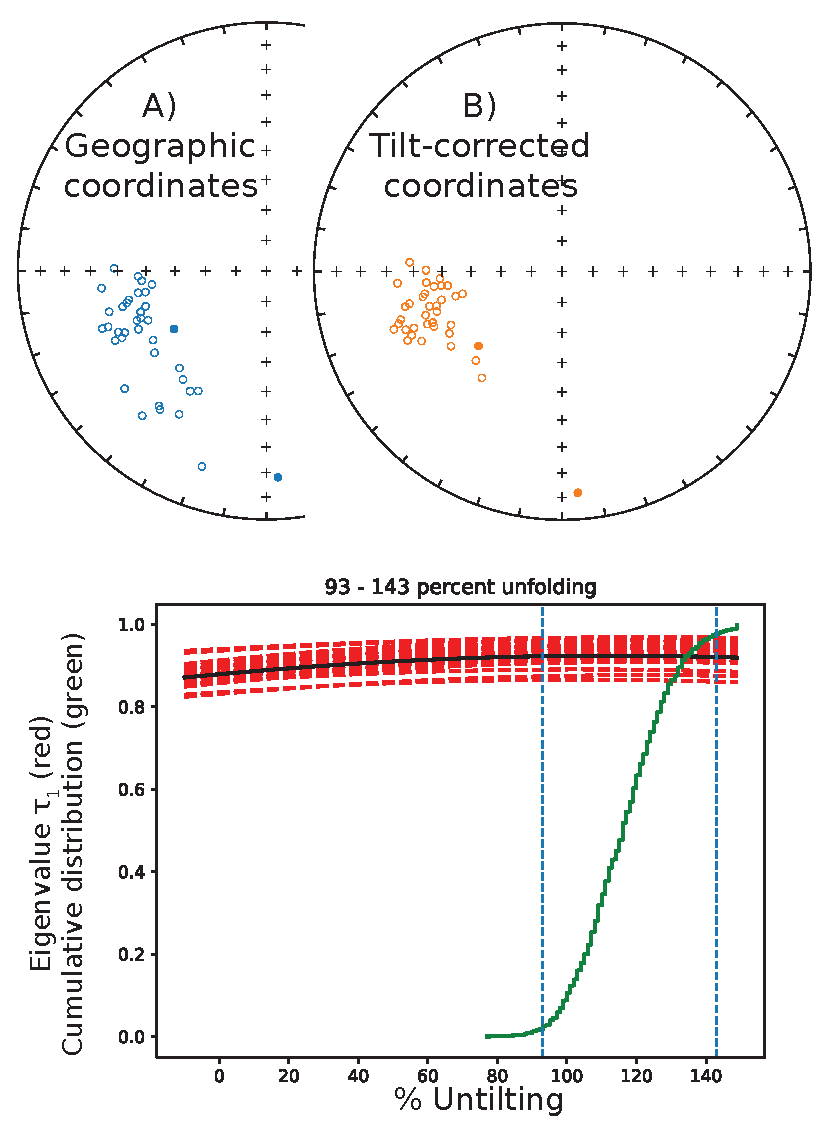
\includegraphics[width=0.6\textwidth]{figure/Zhang2024a/SC1_fold_test.pdf}
\caption[Jacobsville Formation fold test]{Bootstrap paleomagnetic fold test \citep{Tauxe1994a} of the detrital remanent magnetization directions recorded by specimens from the nearly horizontal beds and moderately tilted beds at the Snake Creek tributary. Complete unfolding lies within the 95\% confidence limits of the test, consistent with the magnetization having been acquired prior to tilting.}
\label{fig:fold_test}
\end{figure*}

\subsection{Paleomagnetic reversals}

With the insights gained from the thermal demagnetization results of the Jacobsville fluvial intraclasts and the fold test (Figs. \ref{fig:intraclast_pmag} and \ref{fig:fold_test}), we next investigate the detrital remanent magnetizations for all \textit{in situ} specimens from the five stratigraphic sections (Figs. \ref{fig:Chap_Jacobsville_Geologic_map} and \ref{fig:strat_column}). The DRM directions are plotted by stratigraphic section location in Figure \ref{fig:in_situ_pmag}. As observed in the sparser data of \cite{Roy1978a}, there are dual polarity magnetizations (Fig. \ref{fig:strat_column}). The paleomagnetic polarity reversals are shown in stratigraphic context in Figure \ref{fig:strat_column} with specimen magnetization declinations plotted against stratigraphic heights. The record of Laurentia's paleomagnetic poles from the Proterozoic through the Phanerozoic (see compilations in \cite{Torsvik2012a} and \cite{Swanson-Hysell2021c}) gives a continuity of the orientation of the continent that enables the geomagnetic polarity of the directions to be interpreted. In this framework, the westerly DRM directions are normal geomagnetic polarity and the easterly DRM directions are reversed polarity (Fig. \ref{fig:in_situ_pmag}). 

At the Dover Creek section, which goes along Dover Creek and then up the waterfall of a side tributary (the Hungarian Falls side falls), numerous hematite-rich siltstone to fine sandstone layers commonly occur in association with trough cross-bedded sandstone and conglomeratic facies. These lithofacies are particularly well-exposed along a tributary waterfall to Dover Creek such that 158 samples were collected for paleomagnetic study (Fig. \ref{fig:Chap_Jacobsville_Geologic_map}, \ref{fig:strat_column}), making this section the most densely sampled amongst all the sections. The specimen DRMs show that the geomagnetic field reversed at least nine times during deposition within the section (Fig. \ref{fig:strat_column}). 

The Natural Wall and Hammel Creek sections are in close proximity to the Dover Creek section (Fig. \ref{fig:Chap_Jacobsville_Geologic_map}) and the unique sedimentary facies association of volcanic-clast conglomerate, red siltstone, and coarse arkosic sandstone is similar to the basal $\sim$120 meters of the section at Dover Creek (Fig. \ref{fig:strat_column}). Our sampling at these two localities is more limited due to there being poorer exposures of siltstone and fine-grained sandstone beds in these sections (Fig. \ref{fig:strat_column}). At Hammel Creek, 16 samples from two siltstone layers near the base of the section are of reversed polarity (Fig. \ref{fig:strat_column}). Near the top of the Natural Wall section, consistent normal-polarity directions are recorded by 15 samples (Fig. \ref{fig:strat_column}). 

At the Snake Creek tributary (Fig. \ref{fig:Chap_Jacobsville_Geologic_map}), 71 specimens yielded interpretable DRMs through multiple levels along the $\sim$95-meter-thick section and all show normal-polarity directions (Figs. \ref{fig:in_situ_pmag} and \ref{fig:strat_column}). At Agate Falls (Fig. \ref{fig:Chap_Jacobsville_Geologic_map}), clay-rich detrital mica-bearing siltstone layers occur through $\sim$30 meters of strata that are incised by the Middle Branch Ontonagon River (Fig. \ref{fig:Field_photo}). 67 total paleomagnetic samples were collected on both sides of the waterfall (Fig. \ref{fig:strat_column}). At least three geomagnetic polarity reversals occurred during deposition within the Agate Falls section (Fig. \ref{fig:strat_column}). 

\begin{figure*}[h!]
\centering
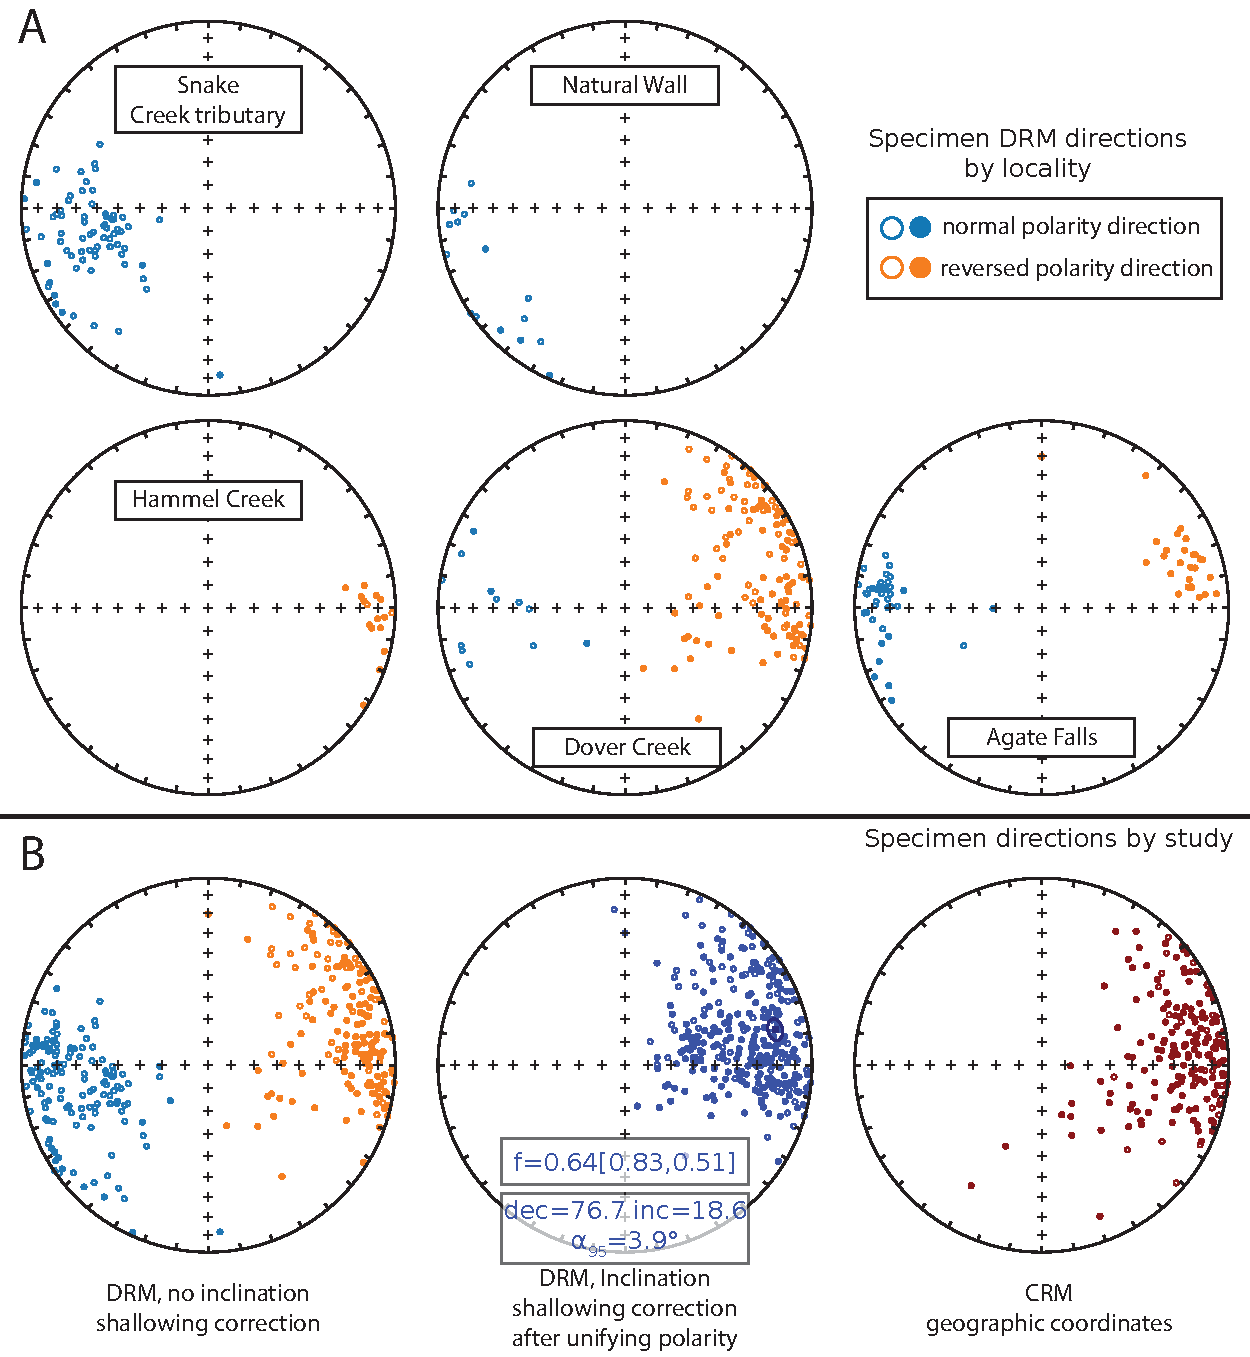
\includegraphics[width=0.78\textwidth]{figure/Zhang2024a/in_situ_pmag.pdf}
\caption[Summary figures for paleomagnetic results from the Jacobsville Formation]{\scriptsize (A) Specimen detrital remanence directions (DRM) plotted by locality on equal area plots. During sample collection, we optimized for vertical stratigraphic coverage such that each sample constitutes a single horizon and therefore a paleomagnetic site. Specimens from the Snake Creek tributary as a mean direction of dec=256.0\textdegree, inc=-30.5\textdegree, k=9.9, $\alpha_{95}$=5.6\textdegree, n=71; the Natural Wall section has a mean direction of dec=242.4\textdegree, inc=-6.4\textdegree, k=9.0, $\alpha_{95}$=13.5\textdegree, n=15; the Hammel Creek section has a mean direction of dec=94.1\textdegree, inc=8.7\textdegree, k=30.7, $\alpha_{95}$=6.8\textdegree, n=16; the Dover Creek section has a mean direction of dec=73.2\textdegree, inc=5.4\textdegree, k=5.6, $\alpha_{95}$=5.6\textdegree, n=138; the Agate Falls section has a mean direction of dec=83.4\textdegree, inc=13.0\textdegree, k=13.4, $\alpha_{95}$=4.9\textdegree, n=67. All reported directions are calculated in tilt-corrected coordinates and after unifying polarity. The measurement-level data are available in the MagIC database (\url{https://doi. org/10.7288/V4/MAGIC/19780}). (B) Summary equal area plots at the study-level combining directions from all localities. The elongation/inclination (E/I) method \citep{Tauxe2004b} was used to estimate the amount of inclination shallowing in Jacobsville specimen DRMs after unifying the polarities (flipping the normal [blue] directions to their antipodes). Details on inclination shallowing corrections are shown in Figure \ref{fig:EI_results} with the value of $f$=0.64 used for the directions in the middle panel. All DRM directions are shown in tilt-corrected bedding coordinates. The summary plot of all specimen chemical remanence directions (CRM) are shown in geographic coordinates show well-grouped reversed-polarity directions whose directions are similar to the DRMs. }
\label{fig:in_situ_pmag}
\end{figure*}

The paleomagnetic reversal test assesses whether two directional data sets share a common mean when one of the polarity directions is flipped to its antipode. Although the occurrence of multiple geomagnetic field reversals during deposition of the Jacobsville Formation is evident (Figs. \ref{fig:strat_column} and \ref{fig:in_situ_pmag}), the limited and often discrete records of many polarity chrons are insufficient for pair-wise reversal tests within single sections (Fig. \ref{fig:strat_column}). Sedimentation within individual siltstone horizons was likely quite rapid given their deposition within fluvial floodplains potentially without sufficient time to average out secular variation within discrete siltstone intervals. We combine all normal and reversed directions from the five sections and perform a reversal test. The \cite{McFadden1990a} reversal test results show the angle between the two mean directions (15.9\textdegree; no inclination shallowing correction) exceeds the critical angle (7.5\textdegree) (Fig. \ref{fig:Jacobsville_reversal_test}), thereby failing the test. This difference largely arises due to normal (west directed) directions in the Snake Creek tributary section being slightly steeper in their upward inclination. There are at least four possible explanations for this behavior: 1) the lower number of normal directions which dominantly come from the Snake Creek tributary section may not have averaged out secular variation; 2) there could have been plate motion during Jacobsville deposition with the normal polarity in the Snake Creek tributary section being acquired when Laurentia was at a slightly higher latitude; 3) there could be a bias from the reversed CRM superimposed on the normal DRM in the Snake Creek tributary specimens being incompletely removed during thermal demagnetization; 4) the geomagnetic field in the early Neoproterozoic could have been slightly different than that of more recent times in terms of the dispersion of pole position at distinct time snapshots potentially associated with changes in field intensity. Regardless, the positive intraclast conglomerate test gives confidence that the Jacobsville Formation has a primary detrital remanent magnetization that can be isolated through thermal demagnetization. This result is strengthened through the positive fold test and the broadly antipodal dual polarity data. Additionally, taking the large number of samples together from both polarities to calculate a pole increases the likelihood that the dual polarity pole has averaged out secular variation.

A total of 186 specimens yielded interpretable chemical remanence directions that are of dominantly reversed polarity. These directions are plotted by stratigraphic section location in Figure \ref{fig:Jacobsville_CRM} and are all shown in Figure 6B. That the CRM directions are a secondary remanence component that postdate the deposition of the Jacobsville Formation is supported by the negative intraformational conglomerate test results and failure in the fold test (Figs. \ref{fig:intraclast_pmag}, S4). However, the similarity of the CRM directions (declination=96.2\textdegree, inclination=15.1\textdegree, $\alpha_{95}$=4.2\textdegree, n=186) with the primary DRM directions (declination=76.9\textdegree, inclination=13.4\textdegree, $\alpha_{95}$=3.3\textdegree, n=307, no inclination shallowing correction) indicate that growth of the secondary pigmentary hematite which carries the CRM likely occurred soon after deposition when Laurentia was in a similar paleogeographic position. 

Overall, the multiple geomagnetic field polarity reversals recorded by the Jacobsville Formation constrain that the end of the Keweenawan normal superchron \citep{Driscoll2016b} (which started ca. 1099 Ma; \citealp{Swanson-Hysell2019a}) had to have ended by the onset of Jacobsville deposition.
 
\section{Discussion}
\subsection{Averaging paleosecular variation and correcting for inclination shallowing}

Igneous and sedimentary rocks associated with the North American Midcontinent Rift provide a high-resolution record of the ca. 1109 to 1070 Ma Keweenawan Track which tightly constrains the apparent polar wander path for Laurentia in the late Mesoproterozoic (Fig. \ref{fig:pole_plot}; \citealp{Swanson-Hysell2019a}). However, high-quality paleogeographic constraints thereafter are sparser and more uncertain in their age until the ca. 775 Ma Gunbarrel large igneous province \citep{Harlan2003a} and subsequent ca. 775-719 Ma poles from western Laurentia extensional basins \citep{Weil2006a, Eyster2019a}. Developing a new paleomagnetic pole from the Jacobsville Formation presents an opportunity for a well-constrained early Neoproterozoic constraint on Laurentia's paleogeographic position. 

Our high-resolution thermal demagnetization successfully isolated detrital magnetization from the secondary chemical magnetization carried by pigmentary hematite that grew after deposition of the Jacobsville Formation. The scatter in the DRM directions can be interpreted to reflect variations in the geomagnetic field during the deposition of the sediments \citep{Steiner1983a, Tauxe1984a}. The multiple geomagnetic field reversals captured by specimens collected from the Dover Creek and Agate Falls sections support that a prolonged period of time is represented by the specimens given that the duration of geomagnetic polarity chrons are typically on the order of tens of Kyr to Myr timescales (Fig. \ref{fig:strat_column}). Therefore, we combine all specimen detrital remanent magnetizations to calculate a paleomagnetic pole for the Jacobsville Formation.

A challenge in interpreting detrital magnetizations is the issue of correcting for inclination shallowing \citep{King1955a, Tauxe2004b, Bilardello2016b}. Scatter of the specimen detrital remanence directions in tilt-corrected coordinates show elongation parallel to the bedding plane, consistent with them being shallowed (Fig. \ref{fig:in_situ_pmag}; \citealp{Tauxe2004b}). Such a directional distribution is due to rotation of detrital hematite grains during deposition and subsequent compaction, resulting in inclinations recorded by sedimentary rocks having shallower angles than the local field in which they are deposited. If uncorrected, shallower inclinations obtained from sedimentary rocks can result in erroneously low estimates of paleolatitudes, biasing paleogeographic reconstructions. To estimate the amount of inclination shallowing, we apply the statistical elongation/inclination (E/I) method that evaluates the deviation of the distribution of a large number ($>$100) of observed sedimentary paleomagnetic directional data with the predicted distribution given by a statistical paleosecular variation model \citep{Tauxe2004b}. Although the TK03 paleosecular variation model is based on data of relatively recent geomagnetic field variations, it has been shown to be compatible with data from the ca. 1.1 Ga lava flows of the Midcontinent Rift \citep{Tauxe2009a}. Furthermore, \cite{Pierce2022a} showed that applying the E/I method to detrital hematite magnetizations within the ca. 1093 Ma Cut Face Creek Sandstone in the Midcontinent Rift successfully corrects the shallow paleomagnetic inclinations of the sediments to that of the North Shore Volcanic Group lava flows that bracket them. \cite{Pierce2022a} also developed a method, that we use here, to represent uncertainties associated with the amount of inclination shallowing into sedimentary paleomagnetic pole positions which can then be summarized with an elliptical Kent distribution \citep{Kent1982a} rather than a circular Fisher distribution \citep{Fisher1953a}. 

Applying the E/I method to the Jacobsville DRM directions results in an estimate for the flattening factor ($f$ factor) of 0.64 with a 95\% uncertainty range of 0.83 to 0.51 (Figs. \ref{fig:EI_results}). The $f$ factor of 0.64 is close to the value of 0.58 which is the mean of inclination shallowing factors compiled for hematite-bearing rocks in \cite{Pierce2022a} (building on compilations of \cite{Bilardello2016b} and \cite{Vaes2021a}). The Fisher mean inclination-corrected detrital remanence mean direction is dec=76.7\textdegree, inc=18.6\textdegree $\alpha_{95}$=3.9\textdegree. The Fisher mean inclination-corrected paleomagnetic pole associated with this nominal $f$ factor is Plon=183.4\textdegree E, Plat=16.9\textdegree S, A$_{95}$=3.1\textdegree. We apply the method of \cite{Pierce2022a} to incorporate the uncertainty in the E/I estimate of the $f$ factor into the uncertainty of the paleomagnetic pole (Fig. \ref{fig:EI_results}). This uncertainty results in more uncertainty associated with paleolatitude which for the pole is along the great circle path between the mean pole position and the locality of the Jacobsville sections. Following \cite{Pierce2022a}, the pole can be represented with a Kent distribution 95\% confidence ellipse which is: mean longitude=183.4\textdegree E, mean latitude=16.9\textdegree S, major axis longitude=255.5\textdegree E, major axis latitude=45.2\textdegree N, major axis magnitude=4.1\textdegree, minor axis longitude=108.1\textdegree E, minor axis latitude=39.9\textdegree N, minor axis magnitude=3.1\textdegree (Fig. \ref{fig:EI_results}; Table \ref{tab:Kent_means}). This pole position is close to the end of the Keweenawan Track (Fig.\ref{fig:pole_plot}) and far away from Laurentia's pole positions during the Paleozoic when there was orogenesis along Laurentia's eastern margin (Fig. \ref{fig:Jacobsville_Appalachian}). This pole position is consistent with the geochronology constraints on the deposition of the Jacobsville Formation and the positive paleomagnetic field tests that the detrital remanence of the Jacobsville Formation was acquired during the earliest Neoproterozoic. 


\begin{figure*}[h!]
\centering
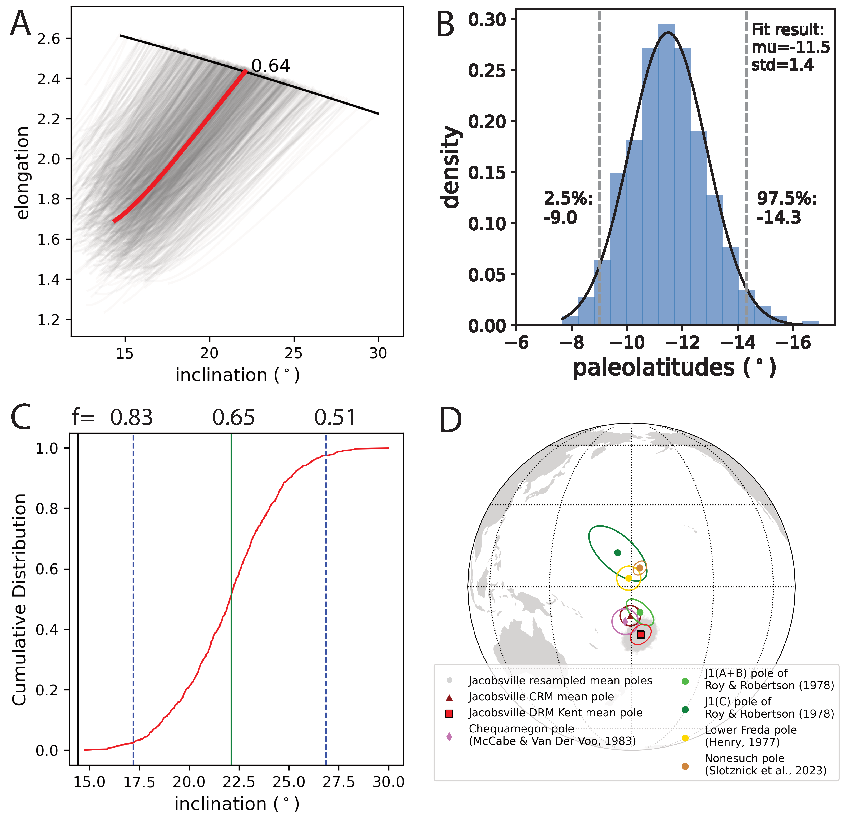
\includegraphics[width=0.8\textwidth]{figure/Zhang2024a/EI_results.pdf}
\caption[Jacobsville Formation inclination shallowing correction]{\scriptsize Results of the estimated amount of inclination shallowing of the detrital remanent magnetization of the Jacobsville Formation using the elongation/inclination (E/I) method \citep{Tauxe2004b}. (A) The E/I method gives an estimated flattening factor $f$=0.64 (red curve) based on where the elongation/inclination curve of the dataset intersects that predicted by the TK03 paleosecular variation model (black curve; \citealp{Tauxe2004b}). The grey lines show 1,000 bootstrap resamples of the DRM directions which provide an estimate of the uncertainty associated with the $f$ factor estimate (95\% interval from 0.83 to 0.51). (B) The distribution of the paleolatitudes resulting from the corrected inclinations of the E/I bootstrap resamples. That the distribution is drawn from a normal distribution with a mean of -11.5\textdegree\ and standard deviation of 1.4 cannot be rejected in the Kolmogorov-Smirnov test. The 95\% confidence bounds shown by dashed lines span a range of paleolatitudes that need to be incorporated into the uncertainty of the reported paleomagnetic pole. (C) The cumulative distribution of inclinations based on the E/I bootstrap results with the 95\% confidence bounds shown in terms of inclination and $f$ factor. (D) The new Kent mean inclination corrected DRM pole (red square) of the Jacobsville Formation is shown in the context of the pole calculated for the CRM (purple triangle) as well as the Jacobsville pole developed by \cite{Roy1978a}, the Chequamegon Formation pole of \cite{McCabe1983a}, and poles from the Oronto Group (Nonesuch Formation, \citealp{Slotznick2023a}; Freda Formation, \citealp{Henry1977a}). The mean pole position of the Kent distribution was calculated following the method of \cite{Pierce2022a}. The close proximity between Jacobsville poles with the Chequamegon pole is consistent with their deposition being coeval. In contrast, the J1 (C) pole of \cite{Roy1978a} developed from hematite-bearing sedimentary rocks in the Sault Ste Marie region plots in the northern hemisphere close to the Freda Formation pole. }
\label{fig:EI_results}
\end{figure*}

\begin{table}[h!]
   \caption{Kent mean paleomagnetic pole for the Jacobsville Formation} 
   \label{tab:Kent_means}
   \footnotesize
   \centering
   \begin{tabular}{p{0.8 in}p{0.8 in}p{0.8 in}p{0.8 in}p{0.8 in}p{0.8 in}}
   \hline
   pole & mean pole position (Plon/Plat) & major axis & major axis 95\% confidence angle & minor axis & minor axis 95\% confidence angle \\
   & $\gamma_{1}$ & $\gamma_{2}$ & $\zeta_{95}$ & $\gamma_{3}$ & $\eta_{95}$ \\
   \hline
   Jacobsville $E/I$ corrected & 183.4\textdegree E / 16.9\textdegree S &  255.5\textdegree E / 45.2\textdegree N & 4.1\textdegree &
   108.1\textdegree E / 39.9\textdegree N & 3.1\textdegree \\
   \hline
 \multicolumn{6}{p{5.5 in}}{Notes: The Fisher mean of the Jacobsville detrital remanence paleomagnetic pole without an inclination shallowing correction is Plon=185.5\textdegree E, Plat=14.0\textdegree S, A$_{95}$=2.7\textdegree; the Fisher mean of the Jacobsville detrital remanence paleomagnetic pole with an inclination shallowing correction of $f$=0.64 is Plon=183.4\textdegree E, Plat=16.9\textdegree S, A$_{95}$=3.1\textdegree; the Fisher mean of the Jacobsville chemical remanence paleomagnetic pole is Plon=179.6\textdegree E, Plat=10.2\textdegree S, A$_{95}$=3.6\textdegree}
   \end{tabular}
\end{table}

\cite{Roy1978a} also studied the paleomagnetism of sedimentary rocks grouped as the Jacobsville Formation and isolated a characteristic magnetization component via alternating-field, thermal, and chemical demagnetization on a suite of Jacobsville red beds near the Keweenaw Peninsula (their area A), the town of Marquette (their area B), and Sault Ste Marie (their area C). Although least-squares principal component analyses was not a routine approach in fitting paleomagnetic directions at the time, that study had success in removing the present day local field overprint and was able to resolve dual magnetic polarities at one locality. The mean paleomagnetic pole position calculated from the interpreted primary magnetic remanence from rocks of the Keweenaw Peninsula and Marquette area (J1 A+B pole; pole longitude=183\textdegree E, pole latitude=9\textdegree S, dp=3\textdegree, dm=6\textdegree; no inclination correction; Fig. \ref{fig:EI_results}; \citealp{Roy1978a}) is in the southern hemisphere and lies close to the mean pole from this study (Fig. \ref{fig:EI_results}). However, their mean pole developed from fine- and medium-grained sandstone near Sault Ste Marie lies in the northern hemisphere with a pole latitude of 12\textdegree N (Fig. \ref{fig:EI_results}). Despite the large uncertainty ellipse associated with this mean pole position, it is distinct from the mean pole position from the Jacobsville Formation in northern Michigan. Instead, it overlaps with the Oronto Group paleomagnetic poles of the ca. 1070 Ma lower Freda Formation and the ca. 1075 Ma Nonesuch Formation (Fig. \ref{fig:EI_results}; \citealp{Henry1977a, Slotznick2023a}). As suggested by \cite{Dubois1962a} and \cite{Roy1978a}, these data suggest that the fluvial red beds in the Sault Ste Marie area that are often taken to be correlative to the Jacobsville Formation \cite[e.g.][]{Malone2020a} are likely time equivalent to sedimentary rocks of the Oronto Group and deposited during post-rift thermal subsidence. 

Deposition of Bayfield Group sedimentary rocks in northern Wisconsin (west of the studied exposures; Fig. \ref{fig:Chap_Jacobsville_Geologic_map}) has been hypothesized to be coeval with the Jacobsville Formation \citep{Hamblin1958a, Kalliokoski1982a, Malone2016a}. Published low precision detrital zircon U-Pb dates developed by laser ablation–inductively coupled plasma–mass spectrometry (LA-ICP-MS) dates are consistent with this interpretation with a maximum depositional age of ca. 1035 Ma for the Chequamegon Formation of the Bayfield Group \citep{Craddock2013a}. Our updated Jacobsville pole position is close to a pole developed from the Chequamegon Sandstone of the Bayfield Group (Fig. \ref{fig:EI_results}; pole longitude=177.7\textdegree E, pole latitude=12.3\textdegree S, A$_95$=4.6\textdegree; no inclination correction; \citealp{McCabe1983a}). These data are consistent with the Bayfield Group being deposited within a contiguous syn-orogenic basin with the Jacobsville Formation during the Rigolet phase of the Grenvillian orogeny. This interpretation can be evaluated with further high-precision geochronology focused on the Bayfield Group. 

\subsection{Age of the Jacobsville Pole}

At the western edge of the Jacobsville bedrock belt in northern Michigan, the formation is in angular unconformity with Midcontinent Rift rocks that were uplifted and tilted prior to Jacobsville deposition (Fig. \ref{fig:Chap_Jacobsville_Geologic_map}; \citealp{Hedgman1992a, Cannon1995a}). Rb-Sr thermochronologic data developed from Paleoproterozoic to Archean lithologies that were exhumed along the Marenisco Fault along with Midcontinent Rift strata in this region indicate that this uplift occurred ca. 1050 Ma associated with the Ottawan phase of the Grenvillian orogeny \citep{Cannon1993a}. Field observations reveal erosional contacts and development of paleosols between the Jacobsville Formation and underlying Midcontinent Rift volcanic rocks at the Sturgeon River within the bedrock belt \citep{Hamblin1958a, Zbinden1988a}. Seismic reflection data beneath Lake Superior have been also been interpreted to indicate that the Jacobsville Formation lies in angular unconformity atop sedimentary rocks of the Oronto Group \citep{Cannon1989a}. This context requires that there was ca. 1050 Ma contractional deformation of Midcontinent Rift strata, erosion of these tilted strata, and renewed subsidence prior to the onset of Jacobsville deposition atop them.

Maximum depositional detrital zircon dates are consistent with this history and provide additional constraints. \cite{Hodgin2022a} applied tandem dating where the young population emerging from a large number of low-precision LA-ICP-MS dates are followed by high-precision CA-ID-TIMS analysis. This approach has the advantage of combining the high number of low-precision analyses that can be acquired through LA-ICP-MS with dates developed through CA-ID-TIMS where the deleterious effects of Pb-loss can be mitigated, and more accurate and precise dates can be obtained. These data reveal the youngest zircon at Sandstone Creek near the Keweenaw Fault (Figure \ref{fig:Chap_Jacobsville_Geologic_map}) to have a date of 992.51 $\pm$ 0.64 Ma (2$\sigma$ analytical uncertainty) and the youngest zircon at Agate Falls (Figure \ref{fig:Chap_Jacobsville_Geologic_map}) a date of 1003.21 $\pm$ 2.23 Ma (2$\sigma$). These dates are consistent with the age of syntectonic magmatism in the Grenville orogen associated with the Rigolet phase of the orogeny \cite[e.g.][]{Bussy1995a, Turlin2019a, Jannin2018a} which is a potential source for the grains. Overall, these dates constrain a maximum depositional age of the Jacobsville Formation in the earliest Neoproterozoic. 

While there has been recent success in applying tandem detrital zircon data to obtain maximum depositional ages that are close to true depositional ages \citep{Karlstrom2020a}, the possibility exists that deposition could significantly postdate the youngest dated detrital zircon. A firm minimum depositional age on the age of the Jacobsville is that it is unconformably overlain by the Cambrian Munising Formation whose base was deposited ca. 501 to 497 Ma during the Dresbachian Stage (the Guzhangian Stage in the modern Cambrian time scale) \citep{Hamblin1958a, Haddox1990a}. This unconformity is erosional as it truncates Jacobsville strata and intraformational clastic dikes and can have slight angularity \citep{Hamblin1958a, Haddox1990a}. That the Jacobsville Formation is older than the Munising Formation lends tighter constraints than the Cambrian age itself given the evidence discussed above that Jacobsville deposition was syn-orogenic. The only candidate for such orogenesis is the ca. 1010-980 Ma Rigolet phase of the Grenvillian orogeny given that subsequent Paleozoic orogenesis (e.g. the Ordovician Taconic and Carboniferous Alleghanian orogenies) post-dates deposition of the Munising Formation.

That the Jacobsville Formation is folded in the footwall of the Keweenaw fault, beneath the older Midcontinent Rift volcanic rocks in the hanging wall, provides another opportunity to develop a minimum depositional age. Seeking to obtain such a constraint, \cite{Hodgin2022a} targeted calcite within a Keweenaw Fault breccia that cross-cuts a dense network of zeolite veins and slickenslides that yielded a U-Pb date of 985.5 $\pm$ 35.8 Ma (2$\sigma$). While this calcite date has large analytical uncertainty, it indicates that the fault breccia developed associated with the Grenvillian orogeny and it overlaps with the ca. 1010-980 Ma ages of metamorphism associated with the Rigolet phase of the orogeny \citep{Swanson-Hysell2023a}. It is during this ca. 1010-980 Ma Rigolet phase of the orogeny that the Grenville Front developed \citep{Rivers2008a} which indicates that this was a time period when contractional deformation associated with the orogeny was propagating into the Superior craton. Together, the detrital zircon, sedimentology, and the fault calcite dates are consistent with the Jacobsville Formation being deposited in a syn-orogenic Grenville backbulge basin and subsequently deformed as contraction associated with the Rigolet phase of the Grenville orogeny propagated into the interior of Laurentia. 

Previously, some researchers have interpreted there to have been large-scale regional contractional deformation during the Alleghanian orogeny in the Paleozoic leading to reactivation of reverse faults including the Keweenaw Fault \citep{Craddock2017a}. While the Keweenaw Fault is defined quite broadly in \cite{Craddock2017a}, the evidence put forward that is relevant to the segment in this study region are: 1) an interpreted post-Grenvillian orogeny age for the Jacobsville Formation which would require that the deformation of the formation was associated with subsequent orogenesis; and 2) deformation within two $<$1.5 km diameter outliers of Paleozoic sedimentary rocks that overlie the Jacobsville (Limestone Mountain in Figure \ref{fig:Chap_Jacobsville_Geologic_map}). The data used to argue for a post-Grenvillian depositional age of the Jacobsville Formation were the low-precision LA-ICP-MS detrital zircon dates of \cite{Malone2016a} that have now been superseded by the tandem dates of \cite{Hodgin2022a}. These dates are consistent with syn-Grenvillian deposition. This progress leaves the tilted and/or brecciated Paleozoic strata in the small exposed Paleozoic outliers of the 1.5 x 1 km Limestone Mountain and the neighboring 0.5 x 0.3 km Sherman Hill as evidence of Paleozoic deformation: interpreted to be Paleozoic orogenesis by \cite{Hamblin1958a} and \cite{Craddock2017a} and suggested to be an impact structure by others \citep{Milstein1987a}. The impact origin interpretation builds on previous interpretations of the structure as being cryptovolcanic \citep{Cannon1981a}--a common interpretation for structures that have subsequently been recognized as impact related. The tilt and brecciation of these outliers contrasts with widespread flat-laying Paleozoic sedimentary rocks that overlie the reverse faults that underwent contractional deformation associated with rift inversion in Minnesota \citep{Jirsa2011a}. These strata constrain Paleozoic deformation to have been relatively minor on the scale of 10s of meters rather than the kilometers of uplift associated with the rift inversion along these reverse faults \citep{Boerboom2018a}. Clumped isotope temperatures of $\sim$50\textdegree C from the Neoproterozoic fault calcite, also developed by \cite{Hodgin2022a}, reveal that the Keweenaw fault zone was within a couple kilometers of the surface at the time of late Mesoproterozoic to early Neoproterozoic calcite precipitation. These data are inconsistent with major Paleozoic uplift and support the interpretation that the majority of contractional inversion along the Keweenaw Fault occurred during the Rigolet Stage of the orogeny. 

Our new paleomagnetic data provides additional insights into the timing of Jacobsville deformation in the early Neoproterozoic. At the Snake Creek tributary section which is folded against the Keweenaw Fault (Figure \ref{fig:Chap_Jacobsville_Geologic_map}, \ref{fig:strat_column}), the chemical remanence directions held by pigmentary hematite fail a fold test (Figure \ref{fig:Jacobsville_hct_fold_test}), indicating that the pigmentary hematite holding the remanence grew after deformation of the strata. The mean pole position of the chemical remanent magnetization at the Snake Creek tributary section overlaps with paleomagnetic poles of the Grenville Loop that have been assigned exhumation ages of ca. 970-960 Ma (Figure \ref{fig:Jacobsville_Appalachian}; \cite{Brown2012a}). This chemical remanence pole position and the mean Jacobsville detrital remanence pole position are both far away from Laurentia's pole positions at the times of Paleozoic orogenesis or any younger time in the Phanerozoic (Figure \ref{fig:Jacobsville_Appalachian}). This result indicates that the majority of the tilting of the Jacobsville in the footwall of the Keweenaw Fault could not have occurred during Paleozoic orogenesis such as the Alleghanian orogeny as the chemical remanent magnetization would then be expected to record a direction aligned with the Phanerozoic pole path. Instead, the Rigolet phase of Grenvillian orogeny, which ended by ca. 980 Ma, is the only feasible orogenic interval that could have tilted these strata. This result constrains the Jacobsville Formation in the studied outcrop belt to have been deposited prior to ca. 980 Ma. While Paleozoic reactivation could have occurred, and there could be deformation of that age elsewhere such as at Limestone Mountain, deformation at this time on the Keweenaw Fault would have been relatively minor compared to that in the early Neoproterozoic.

In conclusion, our paleomagnetic data and existing chronological data combined with the geological constraints are most consistent with the interpretation that the Jacobsville Formation within the studied bedrock belt was deposited in a syn-orogenic basin associated with the Rigolet Phase of the Grenvillian orogeny. This syn-orogenic basinal setting, which is consistent with the sedimentology of the formation (Fig. \ref{fig:strat_column}), provides a mechanism for developing accommodation space. The total duration of deposition of the Jacobsville is uncertain with these constraints alone particularly given the low precision on the 985.5 $\pm$ 35.8 Ma calcite date. However, data from the Grenville orogen itself constrain the end of the Rigolet phase to be ca. 980 Ma \citep{Swanson-Hysell2023a}. As the studied sections proximal to the Keweenaw Fault were deformed in its footwall during this phase of contractional deformation, it is reasonable to interpret deposition as occurring before the ca. 980 Ma cessation of Grenvillian orogenesis. Taken together, we consider the best nominal age constraint for the depositional age of the Jacobsville Formation to pair with the Jacobsville paleomagnetic pole position to be ca. 990 Ma as the Rigolet phase of the orogeny was ongoing. While deposition within peripheral foreland basins typically lasts between 10 and 50 million years \citep{Woodcock2004a}, the backbulge depocenter may not be as stable or long-lived. Given the available chronometric constraints from the Jacobsville Formation, the Keweenaw Fault and the Rigolet phase in the Grenville orogen, deposition of the Jacobsville can be considered to have occurred within the 1000 to 980 Ma time interval.

\subsection{Slowdown of Laurentia's plate motion due to the Grenvillian orogeny}

The ca. 1109-1070 Ma Keweenawan Track constrains rapid motion of Laurentia from high latitudes toward the equator (Fig. \ref{fig:Jacobsville_paleogeography}; \citealp{Davis1997a, Swanson-Hysell2019a}). Apparent polar wander path inversion results are consistent with the pole path being dominated by plate tectonic motion that could have reached a rate of 30 cm/yr (95\% interval of 27-34 cm/yr; one Euler pole scenario; \citealp{Swanson-Hysell2019a, Rose2022a}); even faster than the rate of Indian plate motion during the closure of the Neotethys Ocean \citep{Hinsbergen2022a, Jagoutz2015a}. Laurentia's rapid motion preceded and coincided with the onset of the collisional Grenvillian orogeny. In contrast to the rapid changes in pole position associated with the Keweenawan Track, the relatively close proximity between the ca. 990 Ma Jacobsville pole and ca. 1085 to 1070 Ma poles indicate that Laurentia's motion significantly slowed following the onset of the Grenvillian orogeny (Figs. \ref{fig:pole_plot} and \ref{fig:Jacobsville_paleogeography}). Lacking chronostratigraphic constraints, previous treatments have assigned an age to the Jacobsville pole of \cite{Roy1978a} through extrapolation of the motion of the Keweenawan Track \cite[e.g.][]{Li2008a}. With the improved age constraints of \cite{Hodgin2022a} and our new paleomagnetic pole, we can instead constrain that Laurentia's motion decreased by an order of magnitude. Incorporating temporal and spatial uncertainty on the poles gives APWP rate of $\sim$3.2 cm/yr (95\% interval from 2.5 cm/yr to 4.3 cm/yr; Fig. \ref{fig:Jacobsville_Nonesuch_rate}) between ca. 1070 to 990 Ma.  

\begin{figure*}[h!]
\centering
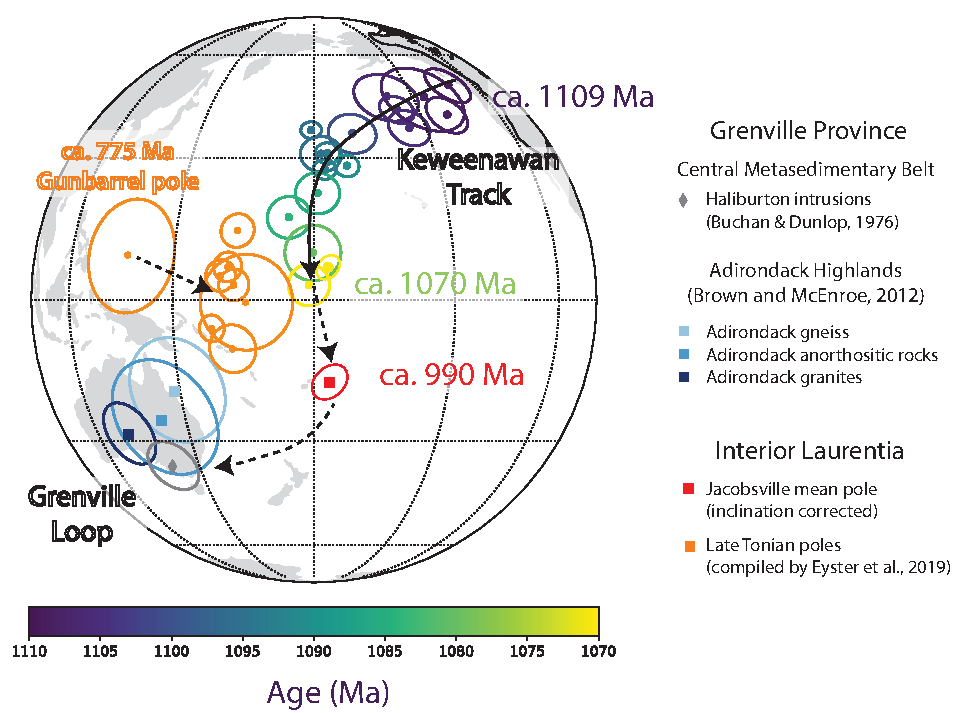
\includegraphics[width=\textwidth]{figure/Zhang2024a/Jacobsville_pole_plot.pdf}
\caption[Jacobsville Formation paleomagnetic pole position in context of the Keweenawan Track and the Grenville Loop]{The inclination-corrected Jacobsville Formation detrital remanent magnetization mean pole position with its Kent uncertainty ellipse is plotted in context of the ca. 1109-1070 Ma Keweenawan Track (poles color-coded by age shown in the colorbar), selected poles from the Grenville Province, and late Tonian poles of Laurentia as compiled by \cite{Eyster2019a} (orange colored poles). The southerly pole position of the ca. 990 Ma Jacobsville Formation indicates that the study area was crossing the equator in the late Mesoproterozoic to early Neoproterozoic. Given the large arc distance between the ca. 990 Ma Jacobsville pole and the poles of the Grenville loop, such as those of the the Haliburton intrusions, we suggest that estimates of their age as $>$1000 Ma \citep{Warnock2000a, Halls2015b, Evans2021b} are likely too old. The solid curve with arrow represents a continuous path of the Keweenawan Track, the dashed curves with arrow represent inferred apparent polar wander in the early Neoproterozoic based on data developed and compiled in this study and by \cite{Eyster2019a}. The pole compilation used in this figure is included as Table S1. }
\label{fig:pole_plot}
\end{figure*}

This slowdown in plate motion is geodynamically consistent with the onset of Grenvillian orogenesis. The earliest records of orogenesis on the leading margin of Laurentia occur ca. 1090 Ma with estimates of peak orogenesis associated with the Ottawan stage of the orogeny occurring ca. 1050 Ma \citep{Rivers2012a, Swanson-Hysell2023a}. Inversions of the Keweenawan Track that incorporate multiple tectonic Euler poles indicate a slowdown from rates exceeding 20 cm/yr prior to 1095 Ma to rates below 20 cm/yr after 1095 Ma \citep{Swanson-Hysell2019a, Rose2022a}. This initial slowdown could be associated with soft collision as contractional deformation initiated on the leading edge of Laurentia \citep{Staal2020a}. Continued contractional collision led to substantially thickened crust recorded by granulite-facies metamorphic rocks by the time of peak Ottawan phase metamorphism ca. 1050 Ma \citep{Rivers2012a}. The large slowdown in plate speed as now constrained by the Jacobsville paleomagnetic pole is associated with this progression to hard continent-continent collision involving increased crustal thickening and progressive transmission of contractional stress that eventually progressed into the interior of Laurentia \citep{Cannon1994a}.

Laurentia's rapid motion was associated with closure of the Unimos Ocean and is consistent with it being on the lower plate that subducted under a conjugate continent (e.g. Amazonia) that collided on its margin (\citealp{Swanson-Hysell2023a}; Fig. \ref{fig:Jacobsville_paleogeography}). The Jacobsville paleomagnetic pole constrains this motion to have slowed as orogeny progressed to be a large-scale continent-continent collision. As a result, Laurentia maintained a low-latitude position throughout the duration of the Grenvillian orogeny which sutured continents together into the supercontinent Rodinia (Fig. \ref{fig:Jacobsville_paleogeography}). 

\subsection{Implications for the age of the Grenville Loop}

Given that the age and pole position of the Jacobsville Formation had been uncertain and lacking other constraints from sedimentary or volcanic rocks, reconstruction of the paleogeography of Laurentia in the early Neoproterozoic has been reliant on paleomagnetic poles developed from metamorphic rocks within the Grenville Province \cite[e.g.][]{Weil1998a}. As is shown in Figure \ref{fig:pole_plot}, paleomagnetic poles of the Grenville Loop plot near Australia in present-day coordinates; forming arc distances ranging from $\sim$35\textdegree\ to more than 50\textdegree\ away from poles at the end of the ca. 1110 to 1070 Ma Keweenawan Track (Fig. \ref{fig:pole_plot}). Determining ages associated with the Grenville Loop poles is crucial for constraining the motion of Laurentia at this time and the configuration between Laurentia and hypothesized conjugate continents such as Baltica within Rodinia \citep{Cawood2017a, Gong2018a, Swanson-Hysell2021c}.

\begin{figure*}[h!]
\centering
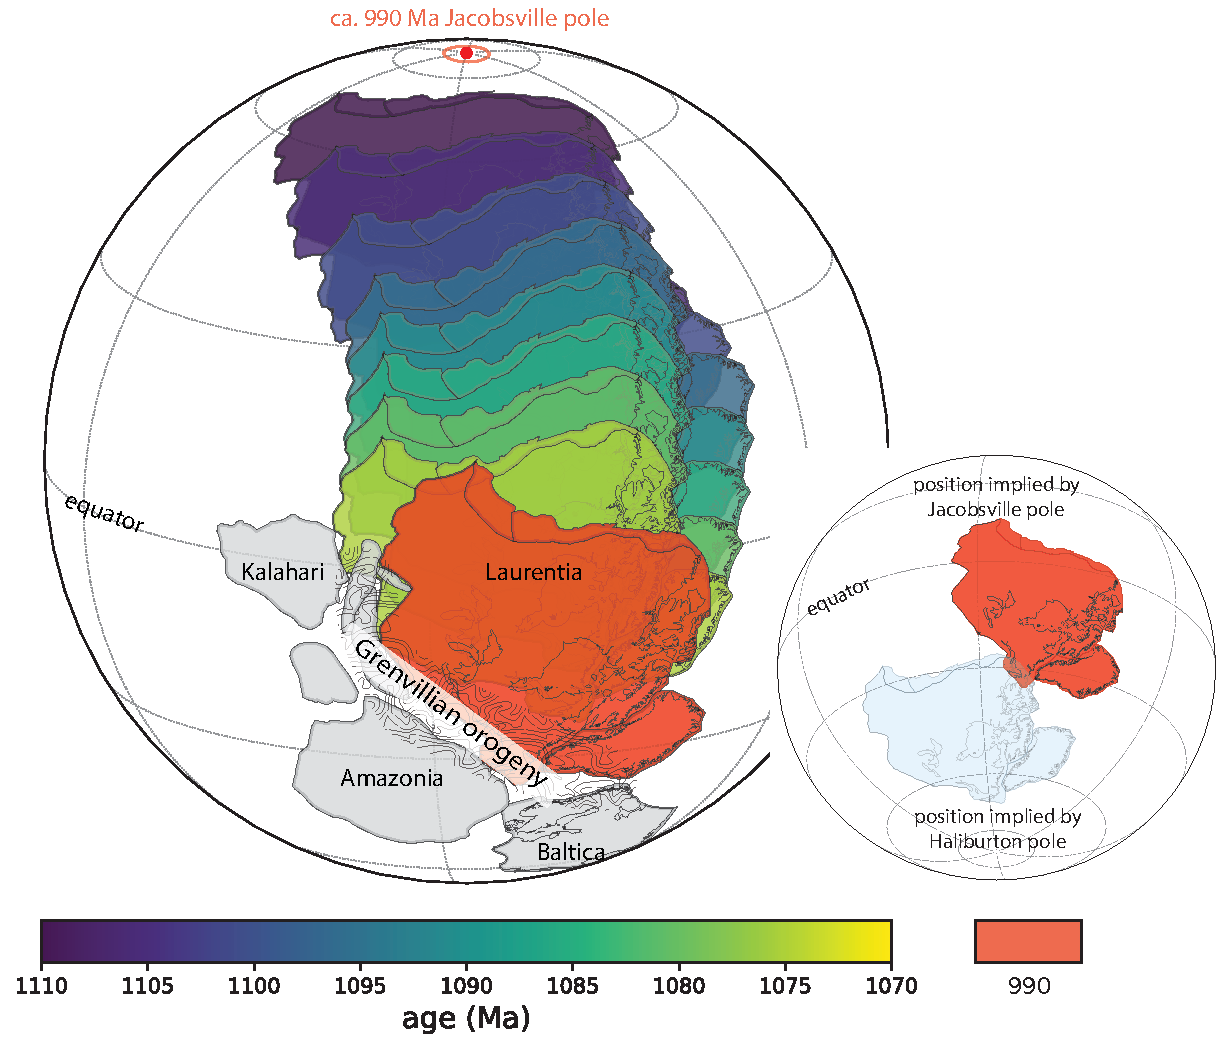
\includegraphics[width=0.8\textwidth]{figure/Zhang2024a/Jacobsville_paleogeography.pdf}
\caption[Paleogeographic position of Laurentia through the late Mesoproterozoic to early Neoproterozoic]{Paleogeographic position of Laurentia through the late Mesoproterozoic to early Neoproterozoic. The color-coded reconstructions show snapshots of Laurentia's position and orientation at 5 Myr intervals from 1110 to 1075 Ma. These reconstructions implement the two-stage tectonic Euler pole rotation inversion of \cite{Swanson-Hysell2019a}. The paleogeographic snapshot colored in red shows the position and orientation of Laurentia ca. 990 Ma as constrained by the Jacobsville paleomagnetic pole developed in this study. Interpreted positions of Laurentia's conjugate continents along its margin are shown in grey. This reconstruction shows that while Laurentia experienced rapid latitudinal changes through the Keweenawan Track that its motion was much slower between ca. 1075 and 990 Ma as the Grenvillian orogeny progressed. The paleogeographic positions of conjugate continents to Laurentia long the Grenville margin in the reconstructions follow the interpretation of \cite{Swanson-Hysell2023a}. The inset figure compares Laurentia's position predicted by the new Jacobsville paleomagnetic pole (red) and that constrained by the Haliburton intrusions of the Grenvillian orogeny (light blue) which has been assigned an age of 1015 Ma \citep{Warnock2000a}). We suggest that this and other Grenville loop poles are younger and that Laurentia traveled from low latitudes toward higher latitudes following ca. 990 Ma while the Grenville orogen was slowly cooling and exhuming.}
\label{fig:Jacobsville_paleogeography}
\end{figure*}

In contrast to rocks of the Midcontinent Rift where magnetizations can be confidently assigned to be the same age as the crystallization ages of the rocks \cite[e.g.][]{Davis1997a,Fairchild2017a,Swanson-Hysell2019a}, rocks of the Grenville orogen experienced up to granulite facies metamorphism (temperatures $>$900\textdegree C; \citealp[e.g.][]{Shinevar2021a, Metzger2021a}) and acquired magnetic remanence during subsequent exhumation \citep{McWilliams1975a, Dunlop1985a, Dodson1985a}. During slow post-orogenic exhumation (1-3\textdegree C/Myr; \citealp[e.g.][]{Rivers2023a}), magnetic minerals acquired remanence by cooling through an extended temperature range over millions to tens of millions of years \citep{Pullaiah1975a, Dodson1980a} or by crystallizing through exsolution \citep{McEnroe2007a}. Determining the age of magnetization in such rocks requires reconstructing cooling histories using isotopic thermochronometers which experience radioisotopic accumulation on mineral-specific closure of elemental diffusion \citep{Dodson1973a, Dodson1985a}. 

Based on the interpretation that blocking of magnetic remanence of the magnetite-bearing Haliburton intrusions of the Grenville Central Metamorphic Belt occurred during relatively narrow temperature ranges close to the Curie temperature of magnetite (i.e. 580\textdegree C), \cite{Warnock2000a} considered that the timing of remanence acquisition during cooling of the intrusions is bracketed between U-Pb titanite and $^{40}$Ar/$^{39}$Ar hornblende dates. As a result, that study interpreted the age associated with the Haliburton paleomagnetic pole to be ca. 1015 Ma. This age has been assigned to the pole in subsequent compilations \cite[e.g.][]{Evans2021a}. In the central Adirondack Highlands of the Grenville orogen, magnetite-bearing granitic rocks and anorthositic rocks record pole positions that overlap with the Haliburton pole while their ages have been interpreted by \cite{Brown2012a} to be ca. 990-970 Ma, based on U-Pb and $^{40}$Ar/$^{39}$Ar thermochronology data developed by \cite{Mezger1991a}. The ca. 990 Ma Jacobsville pole position is both distinct from the Grenville Loop poles and is consistent with a slowdown of Laurentia's plate motion associated with the Grenvillian orogeny (Fig. \ref{fig:pole_plot}). If ages that have been assigned to Grenville Loop poles are taken at face value, those poles represent the position of Laurentia both before and after the position constrained by the ca. 990 Ma Jacobsville pole. Such an interpretation would imply either rapid plate tectonic motion of Laurentia coeval with the Rigolet phase of the Grenvillian orogeny or rapid oscillatory true polar wander \cite[e.g.][]{Evans2003a}. A more straightforward alternative model that could explain the distinct pole positions between the Jacobsville pole and the Grenville Loop poles is that the poles from the Grenville orogen are younger than currently interpreted. Instead of having acquired remanence during the orogeny, the Grenville rocks could have acquired magnetic remanence during protracted exhumation that followed the ca. 980 Ma cessation of contractional deformation associated with the Rigolet stage of the orogeny. In this scenario, the migration of Rodinia to the higher latitude position represented by the Grenville loop poles would have occurred further into the Neoproterozoic after the Grenvillian orogeny had ceased.  

While numerous paleomagnetic data sets have been developed from rocks of the Grenville Province, few are paired with well-calibrated, high-precision thermochronology data. Recent data sets, such as new apatite U-Pb dates of 923 $\pm$ 14 Ma (2$\sigma$ analytical uncertainty) from the Wilberforce pyroxenite \citep{Paul2021a}, give tantalizing hints that temperatures that blocked magnetizations in portions of the orogen were achieved later than the ages assigned to paleomagnetic poles would suggest as U-Pb apatite closure temperatures are close to magnetite blocking temperatures (ca. 360-570\textdegree C; \citealp{Cherniak1991a}). To test the hypothesis that the Grenville Loop is younger than in previous interpretations, geochronology studies are needed to exploit the resolving power of high-precision whole grain analytical methods (i.e. ID-TIMS) and high-spatial-resolution in-situ methods (e.g. laser ablation depth profiling; \citealp{Chew2021a}) for reconstructing the cooling rate and time-temperature history of the Grenville Province. Testing this hypothesis is critical for reconstructions of the paleogeography of Rodinia in the early Neoproterozoic. 

\section{Conclusion}

The magnetization of hematite-bearing fine-grained siliciclastic sedimentary rocks from the Jacobsville Formation can be shown to be detrital and primary through positive intraformational conglomerate and fold tests. We use these data to develop a new inclination-corrected paleomagnetic pole that can be constrained with recently published radiometric age constraints from \cite{Hodgin2022a} to be ca. 990 Ma. This high-quality pole is a crucial addition to Laurentia's apparent polar wander path in the earliest Neoproterozoic. Its position indicates that Laurentia's plate motion significantly slowed during Grenvillian collisional orogenesis. The new pole establishes a well-calibrated constraint for the position of the supercontinent Rodinia in early Neoproterozoic with Laurentia being at the center. The Jacobsville pole implies that ages associated with the paleomagnetic poles recorded by metamorphic rocks of the Grenville Province are likely younger than in current interpretations. Further paired studies of high-quality paleomagnetism and high-precision thermochronology are needed to illuminate Rodinia's motion and configuration in the early Neoproterozoic. 


\section*{Acknowledgments}
Project research was funded by NSF CAREER grant EAR-1847277. Jim DeGraff provided helpful guidance in identifying exposures of the Jacobsville Formation. We gratefully acknowledge the Michigan Department of Natural Resources for sampling permitting. We thank Tim Lyons for additional private land access. We thank Madeline Swanson-Hysell for her assistance in the field. We thank David Malone, Douglas Elmore, and two anonymous reviewers for their helpful reviews. 

\chapter[Paleomagnetism of the southwestern Laurentia large igneous province and Cardenas Basalt: pulsed magmatism during rapid late Mesoproterozoic plate motion][southwestern Laurentia large igneous province]{Paleomagnetism of the southwestern Laurentia large igneous province and Cardenas Basalt: pulsed magmatism during rapid late Mesoproterozoic plate motion}

\let\thefootnote\relax\footnote{Zhang, Y., Anderson, N., Mohr, M.T., Schmitz, M.D., Macdonald, F.A., Nelson, L.L., Thurston, O.G. Guenthner, W.R., Karlstrom, K.E., Swanson-Hysell, N.L. (2024). Paleomagnetism of the southwestern Laurentia large igneous province and Cardenas Basalt: pulsed magmatism during rapid late Mesoproterozoic plate motion. Submitted to JGR: Solid Earth.}

\section{Abstract}

Mafic intrusions, lava flows, and felsic plutons in southwestern Laurentia have been hypothesized to be associated with the emplacement of a late Mesoproterozoic large igneous province. Improved geochronologic data resolve distinct episodes of mafic magmatism in the region. The ca. 1098 main pulse of southwestern Laurentia large igneous province (SWLLIP) magmatism is recorded by mafic intrusions across eastern California to central Arizona. A younger episode of volcanism resulted in eruptions that formed the ca. 1082 Ma Cardenas Basalt---the uppermost unit of the Unkar Group in the Grand Canyon. Using the interpretation that the mafic intrusions within the Unkar Group were feeders to the lavas, a paleomagnetic pole was developed by combining data from the intrusions and the lavas. With the updated geochronological constraints, we develop new paleomagnetic data from mafic sills in the SWLLIP. Overlapping poles between the Death Valley sills and rocks of similar age in the Midcontinent Rift is inconsistent with large-scale Cenozoic vertical axis rotations in Death Valley. We also develop a new paleomagnetic pole from the ca. 1082 Ma Cardenas Basalt (pole longitude=183.9\textdegree E, pole latitude=15.9\textdegree N, A$_{95}$=7.4\textdegree, N=18). The new paleomagnetic data are consistent with the pole path developed from time-equivalent rocks of the Midcontinent Rift, supporting interpretations that changing pole positions are the result of rapid equatorward motion. These data add to the record of Laurentia's rapid motion from ca. 1110 to 1080 Ma that culminated in collisional Grenvillian orogenesis and the assembly of Rodinia. 

\section{Introduction}

The ancient North American craton (Laurentia) has a rich record of Stenian (late Mesoproterozoic) mafic magmatism. In the Midcontinent Rift of the Lake Superior region, punctuated episodes of voluminous intrusions and associated volcanism have been dated between 1109-1084 Ma with high-precision geochronology (Figure \ref{fig:SWLLIP_overview}). Paleomagnetic data from these well-preserved and well-dated rift-related rocks within the Midcontinent Rift make up the majority of the Stenian database of paleomagnetic poles for Laurentia \citep{Evans2021a}. These data provide central constraints on global paleogeography during the assembly of supercontinent Rodinia \citep{Swanson-Hysell2021c, Evans2021b}. 

In southwestern Laurentia, widespread Stenian magmatism led to the emplacement of mafic intrusions and lava flows as well as felsic plutons (Figure \ref{fig:SWLLIP_overview}A; \citealp{Wrucke1966a, Shride1967a, Hendricks1972a, Howard1991a, Bright2014a}). Based on petrologic and geochemical data \cite[e.g.][]{Wrucke1966a, Wrucke1972a, Hammond1986a}, it was previously suggested that the mafic intrusions in the region were contemporaneous. However, in comparison to the Midcontinent Rift where extensive high-precision zircon U-Pb geochronology data have been developed (typically with analytical uncertainties $<$1 Myr; \citealp[e.g.][]{Swanson-Hysell2019a}), most ages from rocks associated with the Stenian southwestern Laurentia magmatism have been relatively imprecise (e.g. as compiled and developed in \cite{Bright2014a}). The broadly overlapping ages, albeit with large uncertainties, of rocks that outcrop in California, Arizona, New Mexico, and Mexico led \cite{Bright2014a} to hypothesize that they could be grouped as the southwestern Laurentia large igneous province (SWLLIP). \cite{Bright2014a} further suggested that a temporal overlap of magmatism in the SWLLIP and in the Midcontinent Rift was the result of a geodynamic linkage. However, the available geochronology data from the SWLLIP at the time was not precise enough to test this relationship with the distinct magmatic intervals within the Midcontinent Rift. 

\begin{figure}[h!]
\centering
\includegraphics[width=0.75\textwidth]{figure/Zhang2024b/overview.pdf}
\caption[Overview of the inferred extent of the southwestern Laurentia large igneous province and compilation of high-precision zircon U-Pb geochronology data]{(A) Map of North America showing the inferred extent of the southwestern Laurentia large igneous province (SWLLIP) modified from \cite{Bright2014a} in light brown color, a more strict version of the inferred extent of the SWLLIP based on encircling sills dated to be ca. 1098 Ma through the high-precision geochronology data of \cite{Mohr2024a} in dark brown, together with the Pikes Peak batholith \citep{Green1992b}, and the inferred extent of the Midcontinent Rift. The inferred trace of the Grenville Front is modified from \cite{Rivers2015a}. The inset boxes show the extent of maps in Figure \ref{fig:geologic_maps}. (B) Summary of high-precision zircon U-Pb geochronology data from southwestern Laurentia \citep{Mohr2024a} and from the Midcontinent Rift, highlighting the Duluth Complex and the associated North Shore Volcanic Group \citep{Swanson-Hysell2019a, Swanson-Hysell2021a}, the Michipicoten Island Formation \citep{Fairchild2017a}. The 1082.6 $\pm$ 0.3 Ma Colorado River Trough sill is located in the Dead Mountains in southeastern California. Each black bar represents a $^{206}$Pb/$^{238}$U zircon weighted mean age. The colored shaded regions associated with the black bars represent uncertainties of the mean ages at 95\% confidence level calculated with a Student's-T multiplier.}
\label{fig:SWLLIP_overview}
\end{figure}
    
Due to sparse geochronology data, temporal relationships between units in southwestern Laurentia are mostly inferred. In the Grand Canyon, it has been hypothesized that thick mafic sills and dikes that intrude Unkar Group sedimentary rocks are feeder systems for the Cardenas Basalt lava flows which are the uppermost unit of the Unkar Group \cite[e.g.][]{Hammond1990a, Timmons2005a}. This hypothesis is based on the spatial proximity and trace and major element concentration similarities of lava flows and nearby intrusions \citep{Larson1994a}. No direct field evidence exists for feeder relations. \cite{Hendricks1989a} considered the sills and flows to be from the same parent magma, but did discuss a possible interpretation that the more differentiated flows erupted later than the emplacement of the sills. Applying the assumption that the extrusive and intrusive rocks were coeval, \cite{Weil2003a} developed a paleomagnetic pole by grouping data derived from thirteen mafic intrusions and three Cardenas Basalt lava flows in the Grand Canyon. Similar directions had previously been developed for two Cardenas lava flows by \cite{Elston1973a}. \cite{Weil2003a} assigned an age of 1090.6 $\pm$ 4.5 Ma (2$\sigma$) to their pole based on an $^{40}$Ar-$^{39}$Ar age they developed from biotite interpreted to have formed within the host Unkar sedimentary rocks during the intrusion of a mafic sill. 

Paleomagnetic data have also been developed from SWLLIP mafic sills that intrude Apache Group sedimentary rocks in central Arizona \citep{Helsley1972a, Donadini2011a}. These studies interpreted sills with normal-polarity paleomagnetic directional data as coeval. \cite{Donadini2011a} developed a mean pole from some normal-polarity sills and considered the age of the pole to be that of a baddeleyite U-Pb age of 1088 $\pm$ 11 Ma (2$\sigma$; age from one sill later published by \cite{Bright2014a}). Although \cite{Harlan1993a} also obtained paleomagnetic samples of mafic sills in the same region with clearer distinction between individual cooling units, that the normal paleomagnetic pole of \cite{Donadini2011a} was reported with paired radiometric age assignment led it to be the pole that is included in recent curated paleogeographic compilations \cite[e.g.][]{Evans2021a}. Other sills in the region record reversed directions with steeper inclinations relative to the normal polarity directions \citep{Harlan1993a, Donadini2011a}. In the field guide of \cite{Donadini2012a}, an age of 1119 $\pm$ 10 Ma (weighted mean of $^{207}$Pb/$^{206}$Pb date of 2 baddeleyite grains) and a age of 1111.6 $\pm$ 8.9 Ma (concordia intercept age of a combination of baddeleyite and zircon dates) were reported for sills of reversed polarity---these geochronology data remain unpublished. Both the steep reversed directions and the geochronological data are consistent with these sills being emplaced during an interval of reversed polarity prior to or during ca. 1109 to 1105 Ma early-stage Midcontinent Rift magmatism \citep{Vervoort2007a, Swanson-Hysell2019a}.

More recently, \cite{Mohr2024a} developed chemical abrasion-isotope dilution-thermal ionization mass spectrometry (CA-ID-TIMS) high-precison U-Pb geochronology data from zircon separated from differentiated zones in thick mafic sills in southwestern Laurentia and from zircon separated by bulk dissolution methods (applying the approach of \cite{Oliveira2022a}) from a thick lava flow within the Cardenas Basalt (Figure \ref{fig:cardenas_strat}). Three sills in Death Valley were dated at 1097.91 $\pm$ 0.29 Ma, 1098.27 $\pm$ 0.27 Ma, and 1098.09 $\pm$ 0.91 Ma, two sills in western Grand Canyon at 1098.16 $\pm$ 0.59 and 1098.09 $\pm$ 0.34 Ma, and one sill in central Arizona at 1097.97 $\pm$ 0.12 Ma (all ages are presented with analytical uncertainties at 95\% confidence which is calculated including a Student’s-T multiplier; \cite{Mohr2024a}). These ages agree with each other within uncertainty (Figure \ref{fig:SWLLIP_overview}B) and suggest that the mafic intrusions across the region were rapidly emplaced in $\sim$0.25 Myr \citep{Mohr2024a}. The data indicate an episode of LIP-style mafic magmatism ca. 1098 Ma in southwestern Laurentia that postdates the early plateau stage of volcanism in the Midcontinent Rift and predates the emplacement of the ca. 1096 Ma Duluth Complex and thick main stage rift volcanics (Fig. \ref{fig:SWLLIP_overview}). The data are consistent with a model where a plume head arrived ca. 1098 Ma under southwestern Laurentia leading to generation of melt and the emplacement of thick mafic intrusions. This plume could have then spread along the base of the lithosphere toward the Midcontinent Rift where it facilitated the reinvigoration of magmatism associated with the emplacement of the Duluth Complex and the North Shore Volcanic Group \citep{Mohr2024a}. In addition, \cite{Mohr2024a} developed a new zircon U-Pb age of 1082.18 $\pm$ 1.25 Ma (95\% confidence) from a Cardenas Basalt lava flow. That age indicates that the eruption of the lavas postdated the widespread ca. 1098 Ma mafic intrusions by $\sim$16 Myr (Figure \ref{fig:SWLLIP_overview}B). Given the rapid apparent polar wander shown by the ca. 1109-1080 Ma Keweenawan Track \citep{Swanson-Hysell2019a}, the $\sim$16 Myr age difference between the Cardenas Basalt and thick mafic sills predict that they should record distinct paleomagnetic pole positions separated by a large angular distance. With the new chronological insights in hand, we develop new paleomagnetic data from the dated mafic sills and additional undated Mesoproterozoic intrusions in Death Valley and the Grand Canyon. We also develop new paleomagnetic data from lava flows of the Cardenas Basalt within the Grand Canyon with an increased number of sites as well as volcanostratigraphic context. 

\section*{Geological Background}
\subsection*{Mafic intrusions in the Crystal Spring Formation, Death Valley}

Rocks in the Death Valley region record the geological evolution of the southwestern margin of Laurentia since ca. 1.8 Ga in the Paleoproterozoic Era (\citealp{Tapani-Ramo1998a}; Figure \ref{fig:geologic_maps}A, \ref{fig:DV_GC_strat_columns}). The basement rocks include Paleoproterozoic para- and orthogneiss \citep{Wasserburg1959a, Barth2000a, Strickland2013a} and early Mesoproterozoic porphyritic quartz monzonite \citep{Labotka1980a}. The Pahrump Group is a 1.5 to 4 km thick mixed carbonate and siliciclastic succession that unconformably overlies these basement lithologies (Figure \ref{fig:DV_GC_strat_columns}; \citealp{Wright1974a, Macdonald2013a}. Formations of the Pahrump Group include the Mesoproterozoic Crystal Spring Formation, the Tonian Horse Thief Springs Formation, the Tonian Beck Spring Dolomite, and the Cryogenian Kingston Peak Formation \citep{Macdonald2013a, Mahon2014a}. A $>$300 Myr unconformity separates the Crystal Spring Formation, which contains mafic sills, and the overlying Horse Thief Springs Formation, which contains $<$775.4 $\pm$ 0.7 Ma detrital zircon (\citealp{Mahon2014a, Dehler2023a}; Figure \ref{fig:DV_GC_strat_columns}) and does not contain the sills. The region experienced Permian-Triassic contraction and magmatism \citep{Snow1991a, Stevens1997a} followed by the Mesozoic Cordilleran orogeny \citep{Burchfiel1992a, Burchfiel1970a, Snow1991a}. Neogene felsic and mafic magmatism (Figure \ref{fig:geologic_maps}), high-angle normal faults, basement detachment faults, as well as transform faults associated with extensional tectonism are widespread in the region \citep{Wright1974a, Snow2000a, Calzia2000a, Wrucke2007a, Renik2013a}. 

\begin{figure}[h!]
\centering
\includegraphics[width=0.85\textwidth]{figure/Zhang2024b/geologic_maps.png}
\caption[Simplified geologic maps of the Death Valley area and the Grand Canyon area]{\footnotesize (A) Simplified geologic map of southern Death Valley, CA, (with units modified from \cite{Workman2003a} and \cite{Wrucke2007a}) showing the location of mafic sills that were sampled for paleomagnetism in this study and geochronology in \cite{Mohr2024a}. The Mesozoic and Cenozoic intrusions that occur in close proximity to the sills have the potential to have resulted in variable degrees of alteration and magnetic overprints. The sills typically were emplaced parallel to host sedimentary beds in the Crystal Spring Formation, but also intrude older crystalline lithologies. In the field, we collected multiple orientation measurements for sills from contact planes or adjacent sedimentary beds. An average orientation was calculated for each sill and was used to tilt-correct the paleomagnetic data. The representative orientations summarized on the map show that different regions are variably tilted. (B) Simplified geologic map of the Grand Canyon with units modified from \cite{Billingsley2000a} and \cite{Billingsley2003a} showing sedimentary rocks of the Unkar Group, mafic sills and dikes that intruded the sedimentary rocks, and the Cardenas Basalt that is the uppermost unit within the Unkar Group (Fig. \ref{fig:DV_GC_strat_columns}) `RM' stands for river mile using the widely adopted nomenclature of tracking distance through Grand Canyon. Bedding orientations at Nankoweap Canyon were collected from lava flow tops and the bedding of the overlying Nankoweap Formation which have very similar orientations; orientations at Lava Chuar Canyon were collected from the lava flow tops; orientations at Basalt Canyon were collected from lava flow tops, interflow sedimentary rocks, and the Dox Formation stratigraphically below the Cardenas Basalt. These bedding measurements were used for tilt-correcting paleomagnetic data. All geochronology data shown are U-Pb zircon ages from \cite{Mohr2024a}.}
\label{fig:geologic_maps}
\end{figure}

Tilting of crustal blocks related to Neogene extension in Death Valley resulted in the exposure of numerous sills and dikes that intrude the basement rocks and the Crystal Spring Formation. The thickness of the mafic sills ranges from $<$1 meter to over a hundred meters \citep{Wright1968a, Hammond1983a}. Chilled margins with the Crystal Spring Formation have a finer grain size than the interiors. Olivine, pyroxene and plagioclase are typically altered within the sills \citep{Hammond1983a}. Based on petrological analyses, \cite{Hammond1983a} interpreted that the alteration dominantly happened during mafic emplacement. Talc deposits up to 30 m thick are developed along contacts between the mafic and the dolomitic lithofacies of the Crystal Spring Formation \citep{Wright1968a}. Mining of talc within these contact metamorphosed zones has resulted in striking white scars in the regional landscape next to some of the sills.

\cite{Heaman1992b} developed U-Pb TIMS dates from baddeleyite separated from pegmatitic zones within two mafic sills that outcrop in the southern Ibex Hills near Saratoga Spring in Death Valley National Park and in the Kingston Range (Figure \ref{fig:geologic_maps}A). Due to Pb loss in baddeleyite, the resultant dates are discordant, with interpreted concordia upper intercept ages of 1069 $\pm$ 3 Ma and 1087 $\pm$ 3 Ma (2$\sigma$). The sill from Saratoga Spring yielded a lower intercept age of ca. 65 Ma which \cite{Heaman1992b} interpreted to be related to growths of younger zircon rims around older baddeleyite crystals. In addition, \cite{Wasserburg1964a} obtained a ca. 235 Ma K-Ar age from a Mesoproterozoic mafic sill in the Crystal Spring Formation that outcrops in Warm Spring Canyon. Although the baddeleyite lower intercept age and the K-Ar age are roughly constrained, these ages are consistent with the mafic sills having been affected by Mesozoic and Cenozoic metamorphism \citep{Snow1989a, Snow2000a}. Recently, \cite{Mohr2024a} extracted zircons from granophyric segregations within two mafic sills from Warm Spring Canyon and one from the central Ibex Range (Figure \ref{fig:geologic_maps}A). High-precision CA-ID-TIMS zircon U-Pb geochronology yielded indistinguishable $^{206}$Pb/$^{238}$U ages of 1097.91  $\pm$  0.29 Ma, 1098.27  $\pm$  0.27 Ma, and 1098.09  $\pm$  0.91 Ma from the three individual sills (95\% confidence; Figure \ref{fig:SWLLIP_overview}B, \ref{fig:geologic_maps}A, \ref{fig:DV_GC_strat_columns}). 

\begin{figure}[h!]
\centering
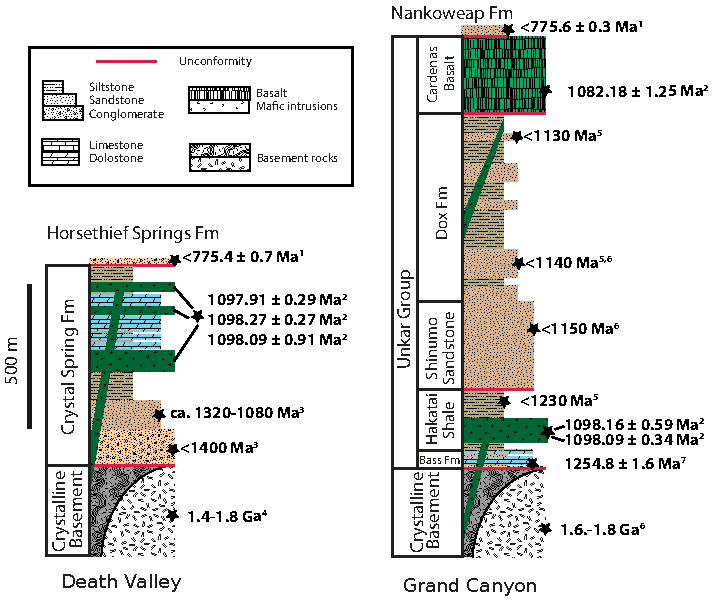
\includegraphics[width=\textwidth]{figure/Zhang2024b/DV_GC_Mesoproterozoic_strat_columns.pdf}
\caption[Simplified regional stratigraphy in Death Valley and Grand Canyon]{\footnotesize Simplified regional Mesoproterozoic stratigraphy in context of older basement rocks and younger Neoproterozoic sedimentary rocks and compiled geochronology in Death Valley and Grand Canyon. Red lines are unconformities. Black stars are existing radioisotopic age constraints. $^1$ CA-ID-TIMS U-Pb detrital zircon dates \citep{Dehler2023a}; $^2$ CA-ID-TIMS U-Pb zircon dates \citep{Mohr2024a}; $^3$ LA-MC-ICPMS U-Pb detrital zircon dates \citep{Mahon2014b}; $^4$ muscovite, biotite, and potassium feldspar $^{40}$K-$^{40}$Ar and $^{87}$Rb-$^{87}$Sr dates \citep{Lanphere1964b}, biotite, muscovite, and hornblende$^{40}$Ar-$^{39}$Ar dates \cite{Labotka1985a}, and SHRIMP U-Pb zircon and monazite dates \cite{Barth2001a, Barth2009a}; $^5$ \cite{Mulder2017a}; $^6$ detrital zircon and detrital muscovite dates \cite{Timmons2005a}; $^7$ TIMS U-Pb zircon dates from an ash layer \cite{Timmons2005a}.}
\label{fig:DV_GC_strat_columns}
\end{figure}

\subsection*{Mafic intrusions in the Unkar Group}

The Grand Canyon Supergroup is divided into the Mesoproterozoic Unkar Group and the Neoproterozoic Chuar Group \citep{Gundy1951a, Elston1989a, Dehler2017a}. The $\sim$2 km-thick Unkar Group contains the Bass Formation, Hakatai Shale, Shinumo Quartzite, Dox Formation, and Cardenas Basalt (Figure \ref{fig:DV_GC_strat_columns}; \citealp{Beus1974a, Elston1989a}). It is interpreted that the Unkar Group dominantly records shallow marine and fluvial depositional environments \citep{Elston1989a, Sears1990a, Hendricks1989a, Timmons2005a}. Siliclastic deposition continued during eruption of the Cardenas Basalt resulting in interflow siltstone and sandstones---often with mudcracks and current ripples respectively  (Fig. \ref{fig:cardenas_strat}). Unkar Group strata typically dip at $\sim$10\textdegree\ to the northeast (Figure \ref{fig:geologic_maps}) toward normal faults that dip $\sim$60\textdegree\ to the southwest \citep{Sears1973a, Timmons2012a}. Intraformational faults and large thickness changes in sedimentary units across faults indicate that the Unkar Group was deposited in an extensional tectonic setting \citep{Sears1990a, Karlstrom1998a, Timmons2001a}. 

Numerous mafic sills and dikes intrude the Unkar Group, but not the overlying Chuar Group (Figures \ref{fig:geologic_maps}B and \ref{fig:DV_GC_strat_columns}; \citealp{Elston1989a}). Sills typically intrude the Bass Formation and the Hakatai Shale of the lower Unkar Group \citep{Hendricks1989a} whereas mafic dikes have been mapped to crosscut the Shinumo Sandstone and the Dox Formation of the upper Unkar Group \citep{Timmons2012a}. Typical dike plane orientations are subparallel to NW-trending faults in the Unkar Group \citep{Huntoon1996a, Timmons2012a}. The sills typically range in thickness between 20 to over 100 meters and are alkali-olivine basalt in composition (\citealp{Hendricks1989a, Larson1994a}; Figure \ref{fig:geochem_major}). Given their spatial proximity and stratigraphic relationship, it had been commonly inferred that all mafic intrusions in the Unkar Group are feeders to the Cardenas Basalt \cite[e.g.][]{Huntoon1996a, Timmons2012a}, though no direct feeder relationships have been observed.

The interior of the thick mafic sills are medium- to coarse-grained with subophitic to ophitic texture characterized by plagioclase and olivine grains being enclosed by poikilitic pyroxenes \citep{Hendricks1989a}. The intrusions are fine-grained at their margins where they are chilled against the Unkar sedimentary rocks.  Some of the sill interiors contain zircon-bearing segregations \citep{Mohr2024a}, which were dated with high-precision CA-ID-TIMS $^{206}$Pb/$^{238}$U at 1098.16 $\pm$ 0.59 Ma at Hotauta Canyon (river mile [RM] 107) and 1098.09 $\pm$ 0.34 Ma at Stone Creek (RM 132) (Figure \ref{fig:SWLLIP_overview}B, \ref{fig:geologic_maps}B; 2$\sigma$ uncertainties). 

\subsection*{Cardenas Basalt}

The Cardenas Basalt at the top of the Unkar Group exclusively outcrops in eastern Grand Canyon (Figure \ref{fig:geologic_maps}). The most complete section of the Cardenas Basalt outcrops at the Basalt Canyon area where $\sim$315 meters of lava flows and associated interflow sedimentary rocks are preserved up to the unconformity between the volcanics and the overlying Nankoweap Formation (Figure \ref{fig:geologic_maps}B, \ref{fig:cardenas_strat}; \citealp{Lucchitta1983a, Hendricks1989a}). Cardenas Basalt also outcrops with variable thicknesses at localities including Lava Chuar Canyon and Nankoweap Canyon (Figure \ref{fig:geologic_maps}B, \ref{fig:cardenas_strat}). The lava flows are typically trachy-basaltic andesite in composition, overall having higher SiO$_2$ values than the mafic intrusions in the Unkar Group (Figure \ref{fig:geochem_major}; \citealp{Hendricks1989a, Larson1994a}).

\begin{figure}[h!]
\centering
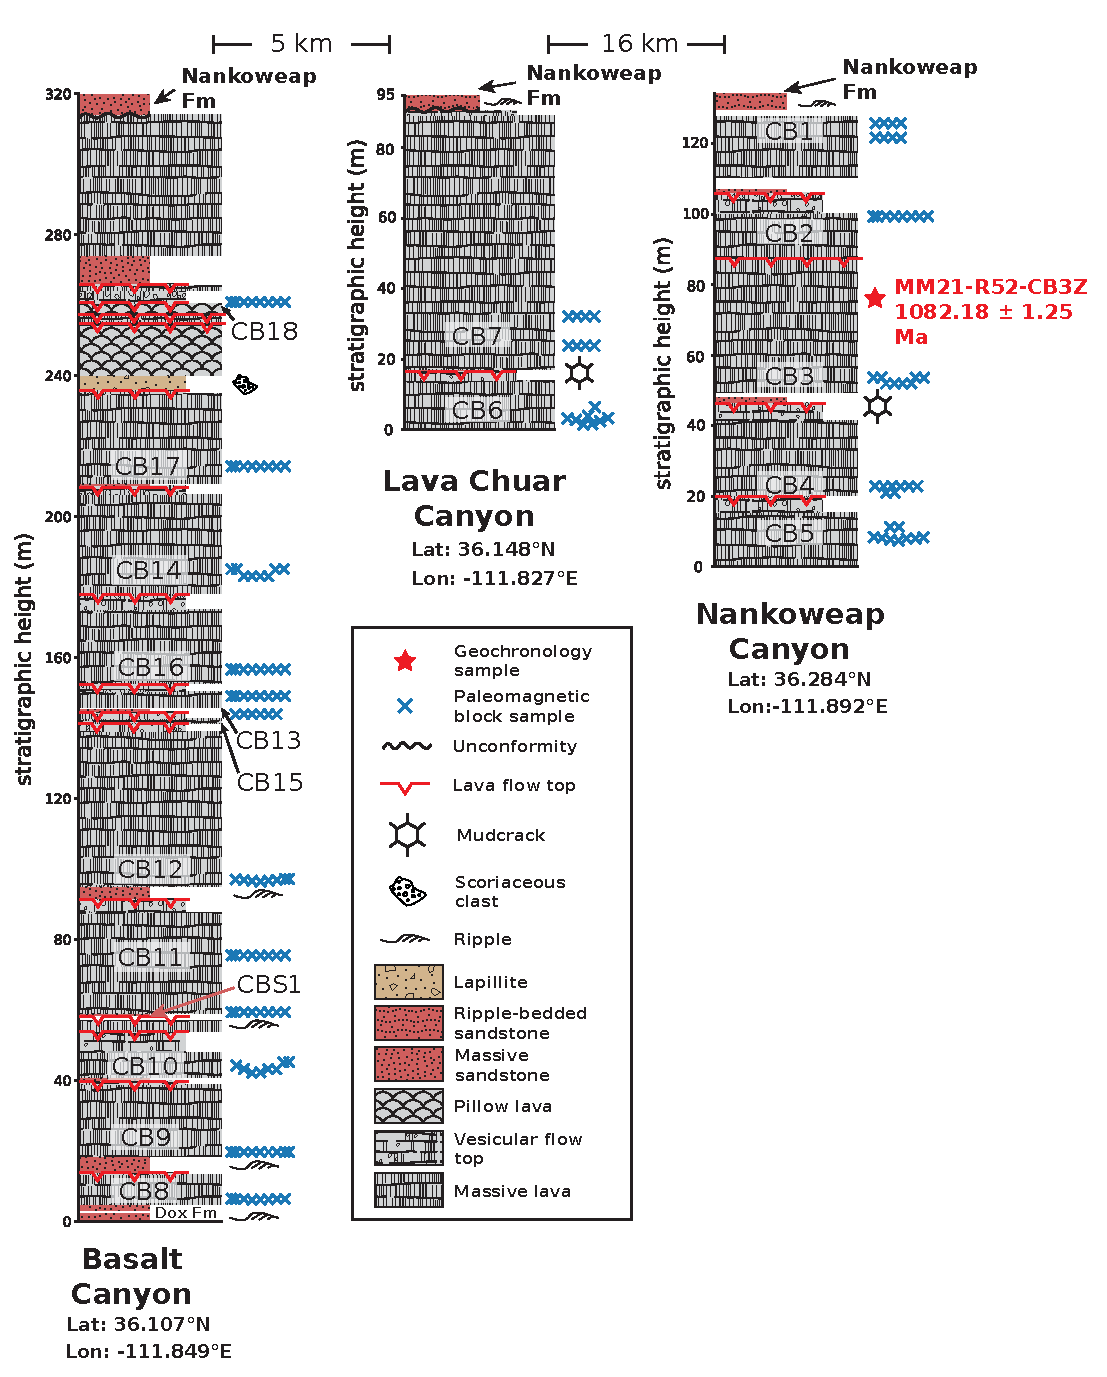
\includegraphics[width=0.82\textwidth]{figure/Zhang2024b/Cardenas_strat_uniform_scale.pdf}
\caption[Volcanostratigraphy of the Cardenas Basalt at Basalt Canyon, Lava Chuar Canyon, and Nankoweap Canyon]{Volcanostratigraphy of the Cardenas Basalt at Basalt Canyon, Lava Chuar Canyon, and Nankoweap Canyon measured in this study. Section locations are shown in Figure \ref{fig:geologic_maps}B. Stratigraphic locations of the collected paleomagnetic samples and the geochronology sample dated by \cite{Mohr2024a} are shown. The interflow sandstones and vesicular lava flow tops distinguish individual lava flows such that paleomagnetic samples from each lava flow constitute a site (labeled as `CB' with distinct numbers). The latitude and longitude values correspond to the base of the stratigraphic sections.}
\label{fig:cardenas_strat}
\end{figure}

Previous studies constructed volcanostratigraphic sections of the Cardenas Basalt at Basalt Cliffs, Ochoa Point, Basalt Canyon, and Lava Chuar Canyon \citep{Lucchitta1983a, Hendricks1989a}. In particular, \cite{Hendricks1989a} developed a stratigraphic section at Basalt Canyon with detailed petrologic and lithologic descriptions. In this study, we investigated three sections at Basalt Canyon, Lava Chuar Canyon, and Nankoweap Canyon (Figure \ref{fig:geologic_maps}). We measured volcanostratigraphic sections with a particular focus on determining individual lava flows that represent distinct cooling units such that paleomagnetic samples collected from a single lava flow are considered to capture the same snapshot of the geomagnetic field as they cooled (i.e. a paleomagnetic site; Fig. \ref{fig:cardenas_strat}). Flow boundaries can be delineated by progressive changes in vesiculation and by highly vesiculated flow tops and/or interflow clastic sedimentary rocks (Figure \ref{fig:cardenas_strat}, \ref{fig:field_photo}E). Interflow sedimentary rocks between lava flows are common (Figure \ref{fig:cardenas_strat}).

At Basalt Canyon, flows in the initial 95 meters are subophitic to ophitic in texture and heavily weathered with a greenish color (Figure \ref{fig:field_photo}B). These flows form slopes characterized by small weathered basalt fragments that often are dislodged pyroxene oikocrysts. Walking on steep slopes mantled by these oikocrysts is like walking on ball bearings. \cite{Walcott1883a} and \cite{Lucchitta1979a} noted that those flows experienced spilitic alteration, interpreted as the result of subaqueous eruptions in a tidal flat or deltaic environment. The claim has also been made that there are pillows in these lower flows \citep{Stevenson1982a, Hendricks1974a}. However, our field observations, as well as those of \cite{Larson1994a} and \cite{Elston1976a}, did not find evidence of pillow lava indicative of subaqueous eruptions in these flows---note that spheroidal weathering can often be misidentified as pillows. While spheroidal weathering, granular grus piles, and ophitic textures on the weathered exposures are common, the features in these basal ophitic flows, including the presence of an observed pahoehoe flow top and basal pipe vesicles, are consistent with them being subaerially erupted sheet flows (Figure \ref{fig:field_photo}B). A ropy flow top consistent with pahoehoe lava flows was also reported in \cite{Hendricks1989a}. The upper 200 meters of Cardenas Basalt flows consist of more competent, cliff-forming lava flows that are finer-grained than the lower sequence. A 4-meter-thick volcaniclastic layer containing cobble- to boulder-sized scoriaceous volcanic clasts surrounded by tan-colored, fine-grained matrix occurs at stratigraphic height of $\sim$240 m (Figure \ref{fig:cardenas_strat}, \ref{fig:field_photo}D). \cite{Lucchitta1983a} named this unit the lapillite member of the Cardenas Basalt and interpreted that it likely formed as pyroclastic debris deposited by lahars. Pillow lavas typically 0.8 to 1 m wide with horizons of volcaniclastic materials consistent with subaqueous eruption are found near the top of the section, above the lapillite layer (Figure \ref{fig:field_photo}F). 

Shorter sections of Cardenas Basalt flows are exposed in Nankoweap Canyon (RM 52) and Lava Chuar Canyon (RM 65) (Figure \ref{fig:geologic_maps}B, \ref{fig:cardenas_strat}). Due to the less complete exposures at these two localities, the volcanostratigraphic correlations between the three localities cannot be unequivocally drawn. However, large lateral variability of individual lava flow thicknesses has been reported \citep{Lucchitta1983a}, indicating that lava flows likely pinch out laterally between the localities. Our stratigraphic sections at the three localities also show variable lava flow thicknesses directly below the Nankoweap Formation (Figure \ref{fig:cardenas_strat}) although this could reflect variability in erosional truncation. We treat the sampled lava flows sampled at different localities as distinct cooling units in this study with each being an individual paleomagnetic site (Figure \ref{fig:cardenas_strat}). The \cite{Mohr2024a} geochronology sample for the Cardenas Basalts comes from the interior of a 57 m thick lava flow at Nankoweap Canyon (Figure \ref{fig:field_photo}A; CB3). Four zircon microlites yielded a weighted mean $^{206}$Pb/$^{238}$U ages of 1082.18 $\pm$ 1.25 Ma (95\% confidence; Figure \ref{fig:SWLLIP_overview}B). 

\begin{figure}[h!]
\centering
\includegraphics[width=0.82\textwidth]{figure/Zhang2024b/field_photo.png}
\caption[Field photos of Cardenas Basalt]{Field photos of Cardenas Basalt. The site names correspond to those shown in the stratigraphic section in Figure \ref{fig:cardenas_strat}. (A) Coarse-grained interior of the 57 m thick CB3 lava flow at Nankoweap Canyon from which zircon were extracted and dated by \cite{Mohr2024a}. (B) Ophitic texture in the interior of flow CB9 at Basalt Canyon. Individual oikocrysts reach diameters of 9 mm. (C) Contact between two individual lava flows CB14 and CB16 (meter level 178 in Fig. \ref{fig:cardenas_strat}) The massive flow bottom of the upper flow is more resistant to weathering than the recessive vesiculated flow top of the underlying flow. (D) The volcaniclastic marker bed containing scoriaceous volcanic clasts surrounded by tan-colored, very fine-grained matrix at 236 to 240 m in the Basalt Canyon section. (E) Amygdaloidal flow top of CB16. Elongate amygdules indicate that vesicles were stretched during flow. (F) Pillow lavas near the top of the exposed stratigraphy at Basalt Canyon (within interval from meter level 240 to 257; Fig. \ref{fig:cardenas_strat}). }
\label{fig:field_photo}
\end{figure}

\section*{Methods}

A total of 123 samples from 15 individual mafic sills were collected from the Death Valley region (Fig. \ref{fig:geologic_maps}A). Core samples were collected with a gasoline-powered drill outside of Death Valley National Park and block samples were collected from sills inside the park. In the Grand Canyon, a total of 184 block samples were collected from 18 individual Cardenas Basalt lava flows, 1 baked interflow sedimentary bed, and 5 mafic intrusions within the Unkar Group. When sampling the intrusions, we preferentially targeted the finer-grained margins of flows and intrusions over the coarser-grained interiors. Typically, 6-9 samples were collected at each site. Both magnetic compass and sun compass were used when orienting the drill cores and block samples in the field. Sun compass orientations were preferentially used when available. In the lab, standard paleomagnetic cores were drilled from the block samples and then oriented relative to the oriented surfaces.

The locations of the paleomagnetic sites are shown in Figure \ref{fig:geologic_maps} and Table \ref{tab:pmag_data}, and the stratigraphic positions of block samples collected from the Cardenas Basalt are shown in Figure \ref{fig:cardenas_strat}. In western Grand Canyon, we sampled the 1098.16 $\pm$ 0.59 Ma sill in Hotauta Canyon as UI4 (RM 107) and the 1098.09 $\pm$ 0.34 Ma Stone Creek Canyon sill as UI5 (RM 132). In the eastern canyon, we sampled the Hance dike north to the Hance Rapids (UI2; RM 77) and the Hance sill south to the rapids (UI3). Another undated mafic sill was sampled at Red Canyon (RM 77) which is south of the river at Hance Rapids along the tributary stream channel of Red Canyon (UI1; Figure \ref{fig:geologic_maps}B). In Death Valley, within Warm Spring Canyon, we sampled the 1097.91 $\pm$ 0.29 Ma sill as CS1 and the 1098.27 $\pm$ 0.27 Ma sill as CS4, and in Ibex Hills, we sampled the 1098.09 $\pm$ 0.91 Ma sill as CS7. Other undated sills are labeled in Figure (\ref{fig:geologic_maps}) and locations for all sites are available in the archived data repository (\url{https://zenodo.org/doi/10.5281/zenodo.10625967}). 

A suite of specimens from sills in the Crystal Spring Formation underwent step-wise thermal demagnetization up to 680 \textdegree C. An additional suite of sister specimens from some samples also underwent thermal demagnetization with an added step of a liquid nitrogen bath following the measurement of natural remanent magnetization. This demagnetization step can preferentially remove overprint magnetization held by multidomain titanomagnetite grains and potentially improve the resolution of the characteristic component. All specimens from the Cardenas Basalt and the mafic intrusions within the Unkar Group underwent step-wise thermal demagnetization up to 580 \textdegree C with some samples continuing up to 680 \textdegree C. The thermal demagnetization protocol had increasingly higher resolution approaching the Curie temperature of magnetite ($\sim$580\textdegree C) and N\'eel temperature of hematite ($\sim$680\textdegree C).

All demagnetization experiments were carried out in the magnetically shielded room at the UC Berkeley Paleomagnetism Lab. The typical magnetic field inside the shielded room is $<$500 nT. An ASC TD-48SC thermal demagnetizer with $<$10 nT field inside the chamber was used for the demagnetization steps. All remanence measurements were made on a 2G Enterprises DC-SQUID superconducting rock magnetometer. The PmagPy software package \citep{Tauxe2016a} was used to implement least-square fits \citep{Kirschvink1980a} to specimen demagnetization data. 

In the Death Valley region, multiple bedding orientations were measured along contacts between the sills and the host sedimentary rocks and along bedding of sedimentary rocks near the sills, and the averages of these measurements were used to tilt-correct paleomagnetic directions of each sill. In the Grand Canyon, the contact planes between the Hance sill and the adjacent sedimentary layers are poorly exposed. We collected bedding measurements from the nearby exposures of the Bass Formation for tilt correction. We also collected orientations from the Hance sill columnar joint planes---planes that are typically vertical prior to tilting. The best-fit plane orthogonal to the columnar joint planes has an orientation similar to the mean bedding plane of the Bass Formation. Bedding orientations of the host Hakatai Shale were used to tilt-correct the Hance dike paleomagnetic data. Bedding orientations were taken on the Cardenas Basalt flow tops and on interflow sediments for tilt correction. All bedding orientation data are available in the archived data repository (\url{https://zenodo.org/doi/10.5281/zenodo.10625967}).

\section*{Results and Interpretations}

Eight out of the 15 mafic sills from the Death Valley area yielded stable, consistent, and interpretable paleomagnetic directional data. All sites including 5 mafic sills, 18 lava flows, and 1 interflow sedimentary bed sampled in the Grand Canyon yielded well-grouped, consistent paleomagnetic directions. The site-level paleomagnetic statistics are summarized in Table \ref{tab:pmag_data}. Data to the individual measurement level are available in the MagIC database (private link for reviewer here: \url{https://doi. org/10.7288/V4/MAGIC/20009}).

\begin{sidewaystable}
\resizebox{0.95\textwidth}{!}{
\tiny
\begin{tabular}{p {1cm} p {2.5cm} p {1.5cm} p {2cm} p {2.3cm} p {0.5cm} p {1cm} p {1cm} p {1cm} p {1cm} p {1cm} p {1cm} p {1cm} p {1cm} }
\hline
site      & study region     & geologic type            & site latitude (\textdegree N) & site longitude (\textdegree E) & n  & dec$_{gc}$                    & inc$_{gc}$                   & dec$_{tc}$ & inc$_{tc}$ & k    & $\alpha_{95}$ (\textdegree) & vgp lat (\textdegree N) & vgp lon (\textdegree E) \\
\hline
CS1$^*$       & Death Valley & sill                 & 35.9688  & -116.9190 & 8  & 303.0                        &  50.0                        & 292.8   & 73.3    & 175  & 4.2  & 41.7     & 203.7    \\
CS2       & Death Valley & sill                 & 35.9651  & -116.9130 & 7  & 290.2                        & 43.2                        & 296.3   & 65.3    & 27   & 11.9 & 42.5     & 187.7    \\
CS6       & Death Valley & sill                 & 35.9618  & -116.8829 & 8  & 275.5                        & -4.7                        & 281.3   & 48.4    & 45   & 8.3  & 25.2     & 172.3    \\
CS7$^*$       & Death Valley & sill                 & 35.8154  & -116.3886 & 2  & 318.0                        & -8.0                        & 331.1   & 42.4    & 167  & 19.5 & 62.7     & 137.2    \\
CS8       & Death Valley & sill                 & 35.8114  & -116.3854 & 9  & 305.2                        & 5.2                         & 297.1   & 58.7    & 78   & 5.9  & 41.1     & 177.8    \\
CS9       & Death Valley & sill                 & 35.8112  & -116.3855 & 5  & 316.0                        & -2.0                        & 317.5   & 52.6    & 39   & 12.3 & 55.1     & 161.9    \\
CS12      & Death Valley & sill                 & 35.7789  & -116.1206 & 8  & 284.7                        & 2.3                         & 301.6   & 63.3    & 30   & 10.2 & 45.5     & 184.3    \\
CS13      & Death Valley & sill                 & 35.8187  & -116.0938 & 3  & 269.0                        & -13.7                       & 293.6   & 51.2    & 150  & 10.1 & 35.8     & 170.3    \\
CB1       & Grand Canyon & lava flow            & 36.2839  & -111.8919 & 8  & 249.3                        & 52.9                        & 270.3   & 51.1    & 200  & 3.9  & 18.4     & 184.5    \\
CB2       & Grand Canyon & lava flow            & 36.2836  & -111.8919 & 8  & 276.3                        & 56.5                        & 283.3   & 78.7    & 329  & 3.1  & 38.2     & 220.8    \\
CB3$^*$       & Grand Canyon & lava flow            & 36.2833  & -111.8928 & 7  & 261.3                        & 58.7                        & 249.3   & 52.9    & 56   & 8.1  & 5.1      & 196.5    \\
CB4       & Grand Canyon & lava flow            & 36.2831  & -111.8928 & 7  & 248.6                        & 35.0                        & 261.3   & 58.7    & 37.1 & 10.0 & 16.9     & 196.9    \\
CB5       & Grand Canyon & lava flow            & 36.2825  & -111.8914 & 9  & 241.6                        & 45.7                        & 276.3   & 56.5    & 71   & 6.2  & 25.3     & 186.8    \\
CB6       & Grand Canyon & lava flow            & 36.1458  & -111.8275 & 8  & 270.3                        & 51.1                        & 252.7   & 47.0    & 88   & 5.9  & 3.8      & 190.7    \\
CB7       & Grand Canyon & lava flow            & 36.1464  & -111.8269 & 8  & 283.3                        & 78.7                        & 269.9   & 42.5    & 106  & 5.4  & 14.1     & 178.5    \\
CB8       & Grand Canyon & lava flow            & 36.1072  & -111.8486 & 8  & 271.9                        & 53.0                        & 272.7   & 38.5    & 132  & 4.8  & 14.7     & 174.5    \\
CB9       & Grand Canyon & lava flow            & 36.1073  & -111.8493 & 8  & 264.6                        & 37.4                        & 283.6   & 27.3    & 96   & 5.7  & 19.3     & 162.3    \\
CB10      & Grand Canyon & lava flow            & 36.1075  & -111.8489 & 7  & 264.0                        & 32.3                        & 273.9   & 38.0    & 88   & 6.5  & 15.4     & 173.6    \\
CB11 \& CBS1 & Grand Canyon & lava flow: sediments & 36.1082  & -111.8489 & 13 & 278.1                        & 28.4                        & 268.3   & 69.5    & 93.2 & 4.3  & 27.2     & 206.5    \\
CB12      & Grand Canyon & lava flow            & 36.1100  & -111.8531 & 8  & 265.9                        & 37.1                        & 268.8   & 42.0    & 193  & 4.0  & 13.1     & 178.8    \\
CB13      & Grand Canyon & lava flow            & 36.1101  & -111.8542 & 7  & 259.9                        & 40.0                        & 267.0   & 6.1     & 107  & 5.9  & -0.6     & 162.4    \\
CB14      & Grand Canyon & lava flow            & 36.1108  & -111.8553 & 7  & 266.0                        & 4.6                         & 259.4   & 52.9    & 514  & 2.7  & 11.6     & 191.3    \\
CB15      & Grand Canyon & lava flow            & 36.1103  & -111.8533 & 6  & 247.4                        & 49.1                        & 263.3   & 45.7    & 89   & 7.1  & 10.7     & 184.1    \\
CB16      & Grand Canyon & lava flow            & 36.1100  & -111.8547 & 7  & 253.6                        & 42.8                        & 266.2   & 17.5    & 63   & 7.7  & 2.2      & 167.6    \\
CB17      & Grand Canyon & lava flow            & 36.1114  & -111.8553 & 8  & 263.2                        & 15.7                        & 264.8   & 49.3    & 253  & 3.5  & 13.5     & 185.9    \\
CB18      & Grand Canyon & lava flow            & 36.1117  & -111.8558 & 7  & 253.6                        & 46.5                        & 285.6   & 52.3    & 98   & 6.1  & 30.2     & 178.9    \\
UI1       & Grand Canyon & sill                 & 36.0247  & -111.9300 & 8  & 243.9                        & 66.1                        & 269.1   & 23.9    & 216  & 3.8  & 6.6      & 168.7    \\
UI2       & Grand Canyon & dike                 & 36.0456  & -111.9183 & 8  & 263.9                        & 19.3                        & 264.0   & 10.0    & 75   & 6.5  & -1.9     & 165.7    \\
UI3       & Grand Canyon & sill                 & 36.0458  & -111.9267 & 8  & 258.1                        & 20.4                        & 264.1   & 25.6    & 139  & 4.7  & 3.2      & 172.4    \\
UI4$^*$       & Grand Canyon & sill                 & 36.2353  & -112.3294 & 7  & 264.0                        & 14.3                        & 314.1   & 51.6    & 54   & 8.3  & 52.2     & 165.4    \\
UI5$^*$       & Grand Canyon & sill                 & 36.3483  & -112.4525 & 8  & 278.2                        & 49.2                        & 295.6   & 49.3    & 76   & 6.4  & 36.8     & 170.8   \\
\hline
\end{tabular}
}
\caption[Site-level paleomagnetic data from mafic sills in Death Valley, Cardenas Basalt, and mafic intrusions in the Unkar Group]{Site-level paleomagnetic data from mafic sills in Death Valley, Cardenas Basalt, and mafic intrusions in the Unkar Group. dec$_{gc}$ and inc$_{gc}$ are site mean declination and inclination in geographic coordinates. dec$_{tc}$ and inc$_{tc}$ are site mean declination and inclination in tilt-corrected coordinates. k represents the Fisher concentration parameter of the site level mean directions. $\alpha_{95}$ represents the Fisher 95\% angular uncertainty of the site level mean directions. \textit{vgp lat} and \textit{vgp lon} represent the latitude and longitude of the site-level virtual geomagnetic poles calculated from tilt-corrected directional data. $^*$ marks sites that have paired high-precision zircon U-Pb ages developed by \cite{Mohr2024a}. CS1 is dated to be 1097.91 $\pm$ 0.29 Ma; CS7 is dated to be 1098.09 $\pm$ 0.91 Ma; UI4 is dated to be 1098.16 $\pm$ 0.59 Ma; UI5 is dated to be 1098.09 $\pm$ 0.34 Ma. All ages are presented with 95\% confidence. }
\label{tab:pmag_data}
\end{sidewaystable}

\subsection*{Death Valley mafic sills}
Thermal demagnetization results on specimens with stable and consistent remanence from the Death Valley sills show that the specimens typically have an overprint component (Figure \ref{fig:demag_plots}). That component can be removed by heating up to $\sim$500\textdegree C, although it is largely removed after heating to 100\textdegree C. The liquid nitrogen demagnetization step (77 K) was also efficient in removing this component. Following the removal of the secondary component, an origin-trending component was resolved through the progressive thermal demagnetization steps up to the Curie temperature of magnetite (i.e. $\sim$580\textdegree C; Figure \ref{fig:demag_plots}).

In geographic coordinates, the site level low-temperature component directions of the Death Valley sills lie very close to the direction of the present-day geomagnetic field direction in Death Valley (Figure \ref{fig:demag_plots}). The low unblocking temperature and the directions of this component are consistent with it being a geologically recent viscous remanence overprint \citep{ Moskowitz1998a, Muxworthy2000a}. On the other hand, the origin-trending component in the sills removed at higher temperatures is directed to the northwest with steep downward inclinations after tilt correction (Figure \ref{fig:demag_plots}). Eight sills yielded consistent results within site and well-grouped mean directions amongst sites. The other sills failed to yield resolvable characteristic directions or consistent results within sites. Figure \ref{fig:poles}A shows the virtual geomagnetic poles (VGP) and the mean pole position (pole longitude=176.6\textdegree, pole latitude=44.9\textdegree, n=8, A$_{95}$=11.8\textdegree; no rotation correction) calculated from the tilt-corrected sills in Death Valley.

\begin{figure}[h!]
\centering
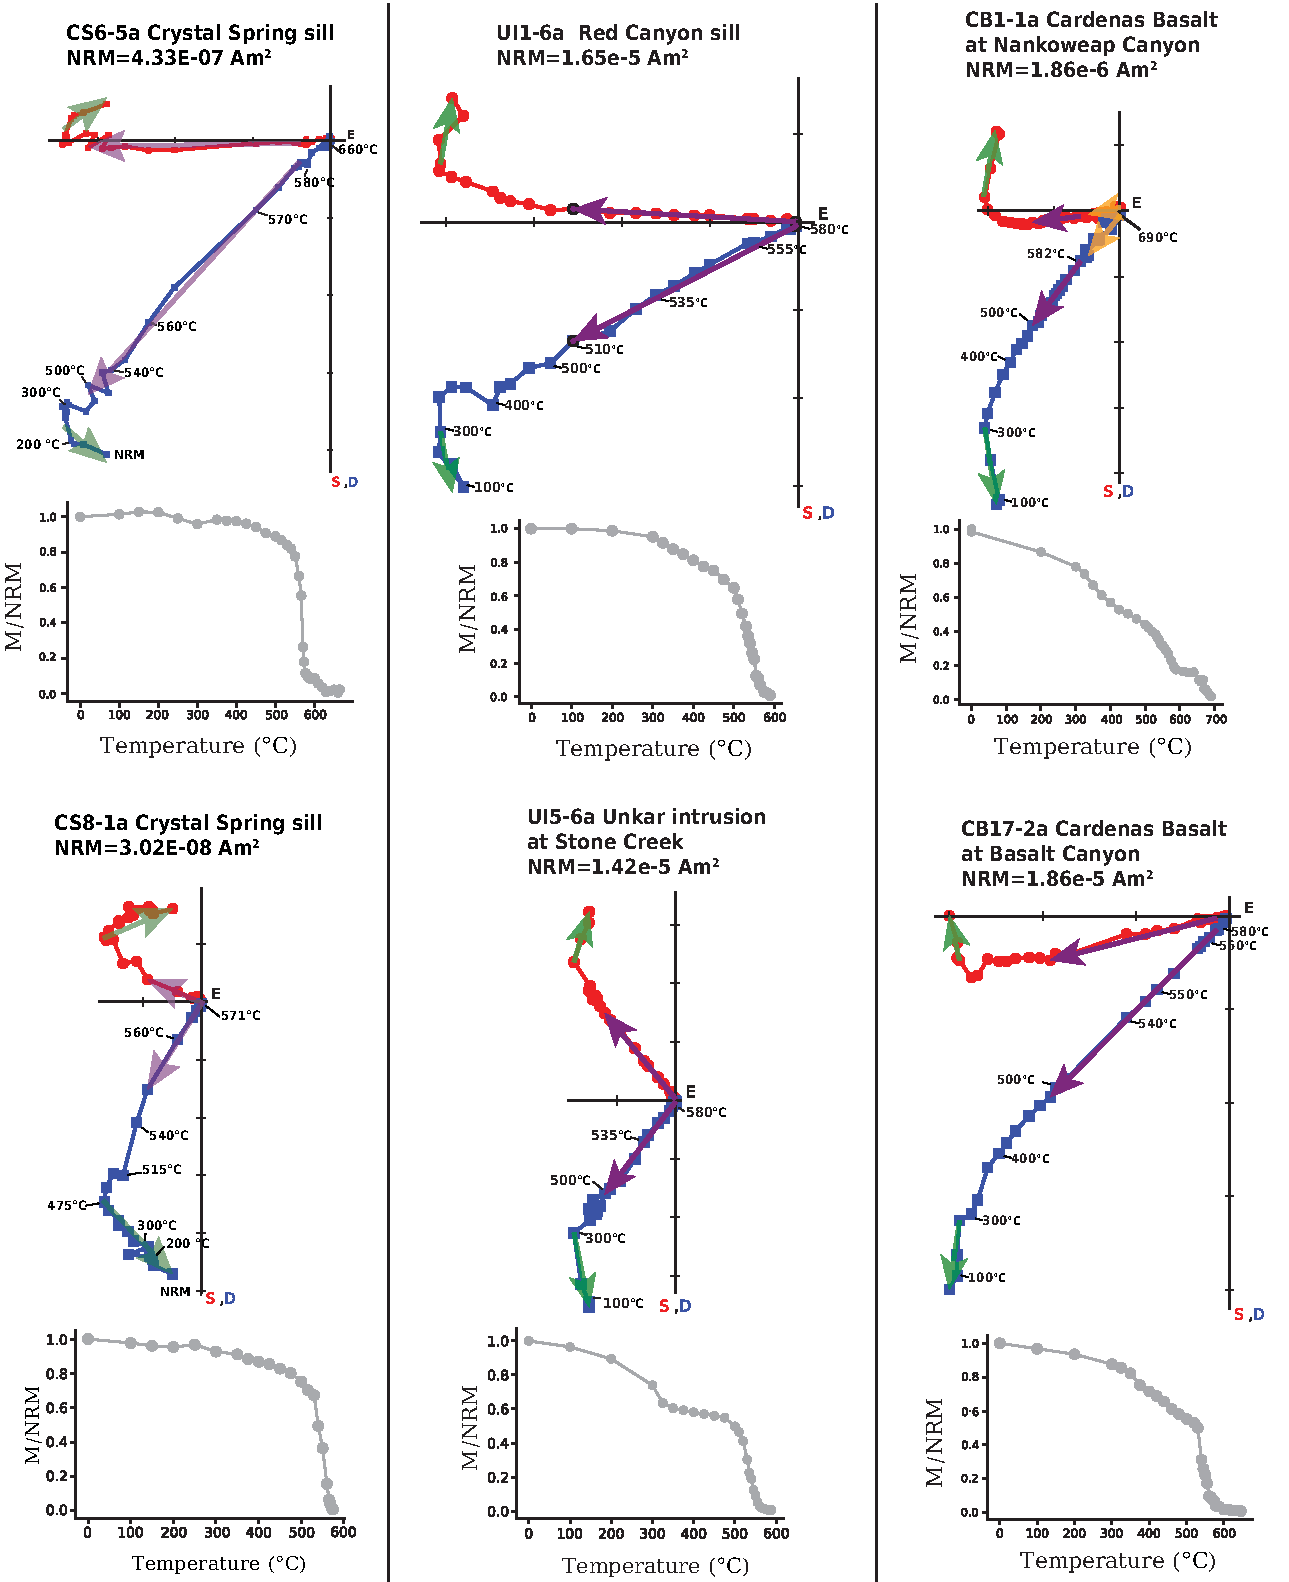
\includegraphics[width=0.78\textwidth]{figure/Zhang2024b/demag_plots.pdf}
\caption[Example orthogonal vector diagrams of specimen thermal demagnetization results]{\footnotesize Example orthogonal vector diagrams of specimen thermal demagnetization results from mafic sills that intruded the Crystal Spring Formation, mafic sills that intruded the Unkar Group, and the Cardenas Basalt. Total specimen magnetic moments (M) normalized by the natural remanent magnetizations (NRM) are plotted against temperature steps. The secondary overprint component (green) in the rocks can be removed by heating typically to $\sim$300\textdegree C, but can be up to $\sim$500\textdegree C, or efficiently removed by liquid nitrogen demagnetization. The interpreted primary component (purple) is origin-trending and typically unblocks sharply through $\sim$500-580\textdegree C. In some Cardenas lava flows such as CB1, a third component that unblocks up to $\sim$690\textdegree C exists, and is interpreted to be carried by hematite that formed during early oxidation. All orthogonal plots are shown in tilt-corrected coordinates.}
\label{fig:demag_plots}
\end{figure}

\subsection*{Intrusions in the Unkar Group and the Cardenas Basalt}
The two dated ca. 1098 Ma sills in eastern Grand Canyon (UI4 and UI5) and three intrusions near Hance Rapids and in Red Canyon (UI1, UI2, and UI3; Figure \ref{fig:geologic_maps}B) all yielded consistent within-site thermal demagnetization results and have similar thermal demagnetization behaviors between sites (Figure \ref{fig:demag_plots}, \ref{fig:equal_area_plots}). Typically, an origin-trending characteristic remanence component unblocks between 500\textdegree C and 585\textdegree C after a secondary overprint component that overlaps with the present local field direction is removed at lower temperatures (Figure \ref{fig:demag_plots}). This thermal demagnetization behavior indicates that the characteristic remanence components in these mafic intrusions are held by low-titanium titanomagnetite. Despite their similar demagnetization behaviors, the mafic intrusions record two distinct groups of remanence directions (Figure \ref{fig:equal_area_plots}). The ca. 1098 Ma mafic sills in Hotauta Canyon (UI4) and Stone Creek Canyon (UI5) record paleomagnetic directions to the northwest with steep inclinations, whereas the other three undated intrusions in eastern Grand Canyon have westerly directions and much shallower inclinations (Figure \ref{fig:demag_plots}, \ref{fig:equal_area_plots}). 

Thermal demagnetization of the 18 Cardenas Basalt lava flows yielded consistent site-level results (Figure \ref{fig:equal_area_plots}). After an overprint component that overlaps with the present local field direction was removed by heating up to 300\textdegree C (Figure \ref{fig:demag_plots}), the specimens typically demagnetized along an origin-trending path approaching the Curie temperature of magnetite. Some specimens continued to demagnetize up to the N\`eel temperature of hematite ($\sim$690\textdegree C; \cite{Ozdemir2006a}; Figure \ref{fig:demag_plots}). The unblocking temperature ranges indicate that (titano)magnetite and hematite are the dominant remanence-carrying minerals in the lava flows. Least-squares line fits made for the magnetite and hematite components have very similar directions in the same specimens (Figure \ref{fig:demag_plots}; CB1-1a). This result is consistent with the hematite having formed due to early oxidation of the lava flows indicating that it acquired remanent magnetization soon after the eruption of the lavas. 

\begin{figure}[h!]
\centering
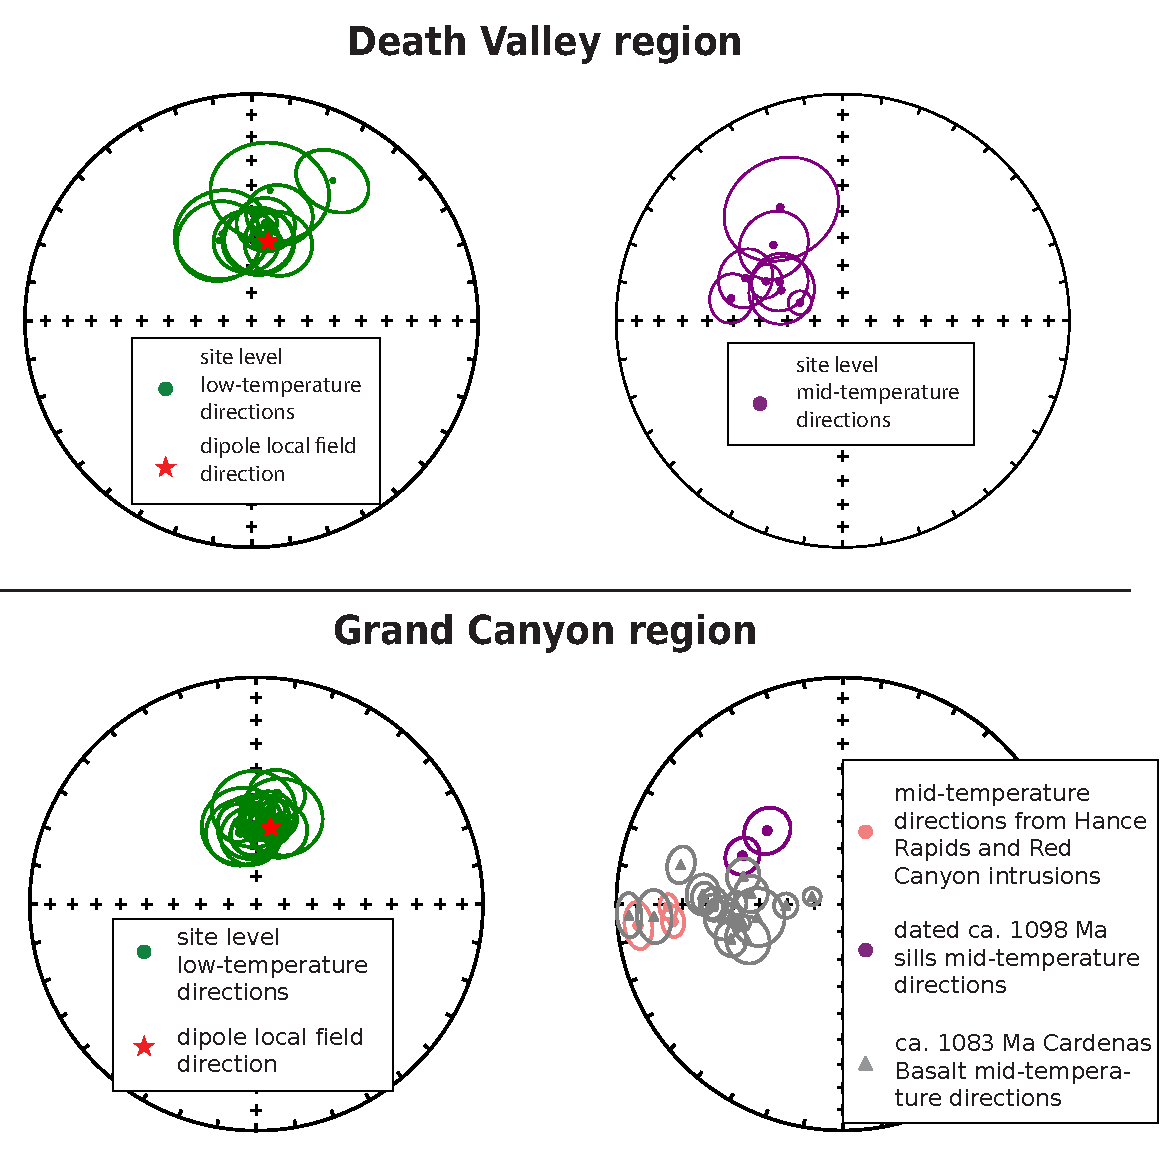
\includegraphics[width=0.8\textwidth]{figure/Zhang2024b/equal_area_plots.pdf}
\caption[equal area diagrams for the site level directional results from the Death Valley region and the Grand Canyon region]{\footnotesize Summary equal area diagrams for the site level directional results from the Death Valley region and the Grand Canyon region. The site level low-temperature components (green) in geographic coordinates are shown in context of present-day local field directions (red star) at the study localities. The mid-temperature directions (i.e. those that unblock over a temperature range consistent with magnetite) are shown in tilt-corrected coordinates. Note that the specimen directions from the mafic sills at Hotauta Canyon (UI4) and Stone Creek (UI5) (directions shown in purple) are more northerly and steeper than the specimen directions of Cardenas Basalt and the intrusions near Hance Rapids (shown in grey and pink).}
\label{fig:equal_area_plots}
\end{figure}

Site-level characteristic directions for all of the intrusions in Death Valley and Grand Canyon as well as Cardenas Basalt flows except for CB4 were calculated using the (titano)magnetite-bearing components. This component isolated through magnetite unblocking temperatures is referred to as the ``mid-temperature direction" in Figure \ref{fig:equal_area_plots}. For site CB4, all except for one specimen have antipodal components, both of which we interpret to be carried by hematite. The antipodal directions recorded within the same specimens may be the result of magnetic self-reversal associated with the oxidation of magnetite into maghemite which subsequently inverted into hematite \citep{Swanson-Hysell2011a}. A detailed description of the specimen results for site CB4 is presented in Figure \ref{fig:CB4_reversal_test}. We combine the normal-polarity (i.e. directions pointing southwest and down) directions held by hematite in six samples together with a normal polarity direction carried by titanomagnetite in one sample for calculating a site mean direction for this flow. Seven samples collected from a baked interflow red sandstone layer (site CBS1) within 0.2 m of the base of lava flow CB11 yielded overlapping paleomagnetic directions with those from the overlying lava flow (Figure \ref{fig:SI_CBS1_CB11}). We group the samples from the lava flow and the baked sediments as one site when calculating the mean direction and virtual geomagnetic pole (VGP). Figure \ref{fig:poles}B shows the VGPs of the two dated ca. 1098 Ma sills in eastern Grand Canyon (UI4 and UI5), VGPs of the the Cardenas Basalt sites, the mean pole position calculated for the Cardenas Basalt (pole longitude=183.9\textdegree, pole latitude=15.9\textdegree, N=18, A$^{95}$=7.4\textdegree, K=22.7; no rotation correction) and the VGPs of the intrusions near Hance Rapids and Red Canyon (UI1, UI2, and UI3). 

\section*{Discussion}

\subsection*{Timing of mafic magmatism in the SWLLIP}

Statistically indistinguishable high-precision U-Pb zircon ages from three sills in Death Valley, two sills in the Grand Canyon, and a sill in central Arizona were interpreted in \cite{Mohr2024a} to be consistent with decompression melting of an upwelling mantle plume ca. 1098 Ma. This hypothesis predicts that other thick sills in the region associated with the SWLLIP were also emplaced ca. 1098 Ma. Paleomagnetic directional data can provide another avenue to gain chronological insight on mafic units for which geochronology data have not been or cannot be developed. Rapid changes in Laurentia's pole position between ca. 1110 and 1070 Ma (Fig. \ref{fig:poles}D; \citealp{Swanson-Hysell2019a}) enable such data to provide more informative temporal constraints than at many other time intervals.

The new paleomagnetic data from the dated sills in the Death Valley region and in the Grand Canyon are consistent with their high-precision U-Pb zircon ages. The 1097.91 $\pm$ 0.29 Ma CS1 sill  and the 1098.09 $\pm$ 0.91 Ma CS7 sill in Death Valley and the 1098.16 $\pm$ 0.59 Ma UI4 sill and 1098.09 $\pm$ 0.34 Ma UI5 sill in Grand Canyon have similar VGP positions at high latitudes in present-day coordinates (Figure \ref{fig:poles}A, B). The new paleomagnetic data further show that six additional undated sills in the Death Valley region have directions that are similar to those from the ca. 1098 Ma dated sills (Figs. \ref{fig:equal_area_plots} and \ref{fig:poles}). These data are consistent with all of the preserved Death Valley sills being associated with the ca. 1098 Ma pulse of mafic magmatism. Figure \ref{fig:poles}A shows the mean pole position calculated for all the Death Valley region sills. The pole overlaps within uncertainty with the pole position of the ca. 1096 Ma North Shore Volcanic Group upper southwest sequence of the Midcontinent Rift (Figure \ref{fig:poles}A; \citealp{Swanson-Hysell2019a}). Although the paleomagnetic data of the Death Valley sills have directional uncertainties associated with potential vertical axis block rotations as detailed in the following section, these structural complexities do not take away the interpretation that the steep downward inclinations (Figure \ref{fig:demag_plots}) are compatible with a ca. 1098 Ma age. Additionally, the normal polarity of the magnetizations is consistent with the sills being emplaced during the earliest portion of the ca. 1099 to $<$1075 Ma Portage Lake normal polarity zone \citep{Swanson-Hysell2019a}---a late Mesoproterozoic superchron \citep{Driscoll2016b}. 

\begin{figure}[h!]
\centering
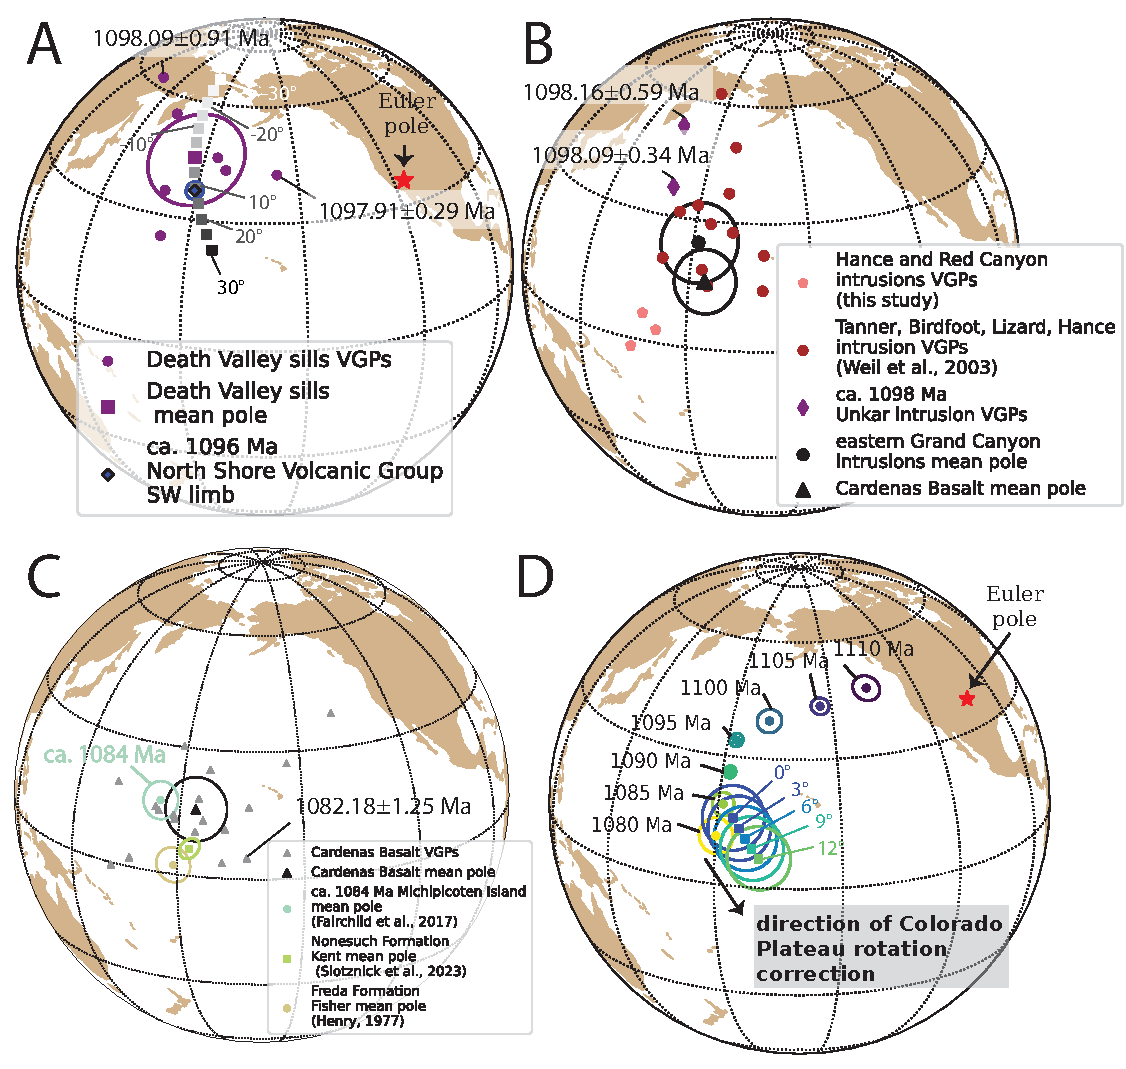
\includegraphics[width=0.8\textwidth]{figure/Zhang2024b/poles.pdf}
\caption[Pole positions of the Death Valley mafic sills, mafic intrusions in the Unkar Group, and the Cardenas Basalt]{\footnotesize (A) Virtual geomagnetic poles (VGP) from the Death Valley mafic sills and the associated mean paleomagnetic pole plotted in context of the paleomagnetic pole position of the ca. 1096 Ma North Shore Volcanic Group southwest sequence pole from \cite{Swanson-Hysell2019a}. Variable vertical axis rotations of the mean Death Valley sills pole about an Euler pole located at 35.8\textdegree N, -116.4\textdegree E are shown. Positive (negative) values represent counterclockwise (clockwise) rotations about the Euler pole. (B) VGPs from the Cardenas Basalt and mafic sills within the Unkar Group are plotted together with the mean Cardenas Basalt pole and the mean pole calculated for intrusions that are hypothesized to be coeval with the Cardenas Basalt. VGPs of intrusions include those developed in this study as well as those from \cite{Weil2003a}. (C) The mean ca. 1082 Ma Cardenas Basalt paleomagnetic pole is plotted together with the ca. 1084 Ma Michipicotan Island Formation paleomagnetic pole \citep{Fairchild2017a} as well as the ca. 1075 Ma Nonesuch Formation pole \citep{Slotznick2023a} and lower Freda Formation pole \citep{Henry1977a}. (D) The Cardenas Basalt mean pole position is corrected for the hypothesized Colorado Plateau rotation with progressively larger rotations about an Euler pole position of -107\textdegree E, 37\textdegree N \citep{Bryan1990a}. The resultant pole positions are plotted in context of the synthesized Keweenawan Track (2 stage pole rotations and true polar wander scenario; \citealp{Swanson-Hysell2019a}). Larger rotations result in less agreement between the Cardenas pole and the pole path based on Midcontinent Rift data. In plots (A) and (C) the VGPs from dated sills and the dated lava flow are labeled with their ages.}
\label{fig:poles}
\end{figure}   

The paleomagnetic pole position of the ca. 1082 Ma Cardenas Basalt plots at a lower latitude distinct from that of the ca. 1098 Ma mafic sills in Death Valley and the western Grand Canyon (Figure. \ref{fig:poles}A, C). Instead, the Cardenas Basalt pole is close to the paleomagnetic pole of the Michipicoten Island Formation of the Midcontinent Rift whose age is tightly bracketed to be between 1084.35 $\pm$ 0.20 Ma and 1083.52 $\pm$ 0.23 Ma \citep{Fairchild2017a}. In addition, the Cardenas Basalt pole is close to the ca. 1075 Ma paleomagnetic poles of the Nonesuch and Freda Formations \citep{Henry1977a, Slotznick2023a} of the Midcontinent Rift Oronto Group. That these localities $\sim$2,500 km apart yield overlapping pole positions when their poles are calculated under the assumption of a time-averaged dipolar field supports interpretations that the field was a stable dipole ca. 1080 Ma. Note that there is uncertainty in the Cardenas pole position associated with hypothesized rotation of the Colorado Plateau in the Mesozoic/Cenozoic (Fig. \ref{fig:poles}D; \citealp[e.g.][]{Bryan1990a}). However, this uncertainty does not take away from the main conclusion as it does not affect interpretations of paleolatitude.

Overall, the large arc distance between the ca. 1098 Ma and the ca. 1082 Ma poles from southwestern Laurentia supports the interpretation based on Midcontinent Rift data that Laurentia experienced rapid plate motion from high latitudes toward the equator in the late Mesoproterozoic \citep{Davis1997a, Swanson-Hysell2009a}. This rapid motion is associated with the closure of the Unimos Ocean which culminating in the onset of Grenvillian collisional orogenesis \citep{Swanson-Hysell2023a}. 

\subsection*{Comparison to Mesoproterozoic paleomagnetic data from central Arizona}

Paleomagnetic data have been developed from mafic sills in central Arizona that intrude the Apache Group sedimentary rocks \citep{Helsley1972a, Harlan1993a, Donadini2011a}. Both \cite{Harlan1993a} and \cite{Donadini2011a} identified sills in the same region that record normal directions and reversed directions with the reversed directions having steeper inclinations. We compiled paleomagnetic data from these two studies with the goal of having each site be a distinct cooling unit. The resultant compilation is provided in Table \ref{tab:SI_Harlan_Donadini_compilation}. The individual site-level directions, corresponding virtual geomagnetic pole positions, and overall mean directions and poles are recalculated by polarity and plotted in Figure \ref{fig:Harlan_Donadini_compilation}. 

The compiled mean pole position of the normal-polarity mafic sills in central Arizona plots near the expected pole position of Laurentia ca. 1095 Ma based on data from the Midcontinent Rift rocks (Figure \ref{fig:Harlan_Donadini_compilation}; \citealp{Swanson-Hysell2019a}). However, the distribution of the normal-polarity virtual geomagnetic pole positions is distinct from a Fisher distribution \citep{Fisher1953a}. Given that these VGPs show an elongate distribution along the Keweenawan Track (Figure \ref{fig:Harlan_Donadini_compilation}), we hypothesize that not all sills were emplaced during the same magmatic episode. However, that the sills have record a normal polarity and one sill yielded a U-Pb baddeleyite age of 1088 $\pm$ 11 Ma \citep{Bright2014a} which has an uncertainty that overlaps with an CA-ID-TIMS zircon U-Pb age of 1097.97 $\pm$ 0.12 Ma from a subhorizonal diabase sill in Salt River Canyon \citep{Mohr2024a} indicate that some of the sills could be coeval with the ca. 1098 Ma mafic sills in Death Valley and Grand Canyon. More precise radiometric dates that is paired with paleomagnetic data are needed from these sills. 

Despite the few records, the central Arizona sills with steep negative inclinations have a mean pole position distinct from that of the normal-polarity sills (Figure \ref{fig:Harlan_Donadini_compilation}). The mean pole plots near the older end of the Keweenawan Track, indicating a high paleolatitude for Laurentia at the time (Figure \ref{fig:Harlan_Donadini_compilation}). This configuration corresponds with the stable high-latitude position of Laurentia between ca. 1140 and 1105 Ma \citep{Ernst1993a, Piispa2018a, Swanson-Hysell2021c}. That reversed polarity is also consistent with the Alona Bay reversed polarity zone which has been identified during the onset of magmatism in the Midcontinent Rift \citep{Swanson-Hysell2019a}. The potential exists that in addition to there being a linkage between a SWLLIP plume that spread to the Midcontinent Rift ca. 1098 to 1096 Ma as hypothesized in \cite{Mohr2024a}, a plume upwelling under Laurentia at the onset of Midcontinent Rift development led to magmatism in both regions. To assess such temporal and dynamic connections, more precise ages of these reversed-polarity sills need to be determined. 

\begin{figure}[h!]
\centering
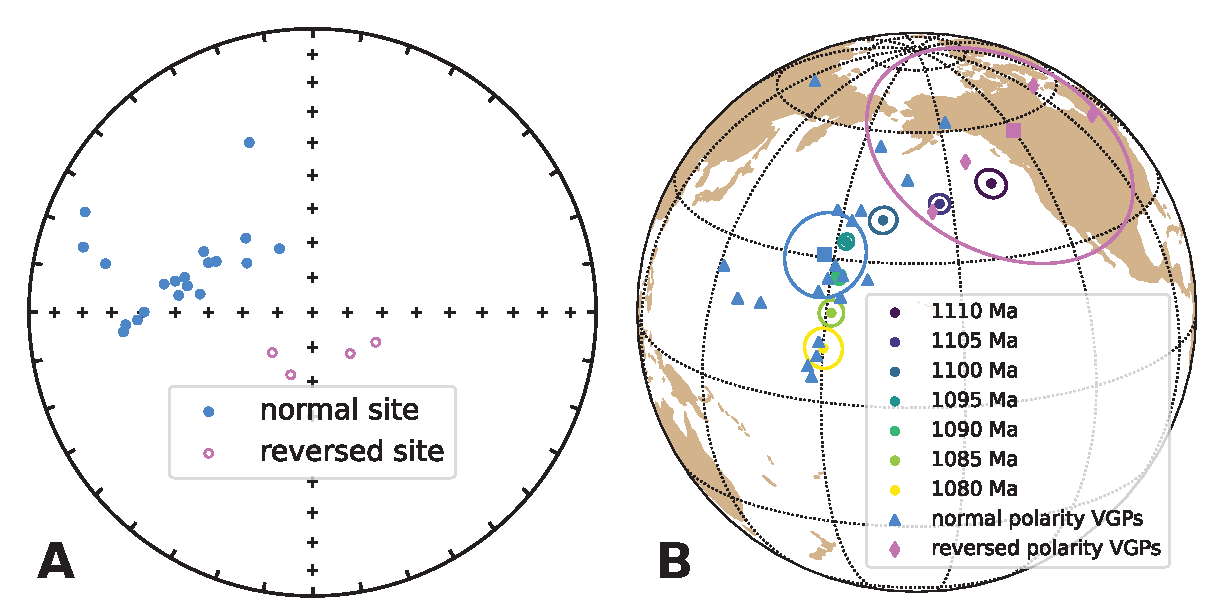
\includegraphics[width=0.8\textwidth]{figure/Zhang2024b/Harlan_Donadini_compilation.pdf}
\caption[Compilation of paleomagnetic data from central Arizona mafic sills]{(A) Compiled paleomagnetic directional data developed by \cite{Harlan1993a} and \cite{Donadini2011a} from mafic sills in central Arizona. The original data are selected with some recalculated such that each site included in this compilation is an individual cooling unit. Some sills record a reversed polarity with steep inclinations (orchid), while the other sills record a normal polarity with shallower inclinations (blue). The compiled data are in Table \ref{tab:SI_Harlan_Donadini_compilation}. (B) Virtual geomagnetic poles (VGP) of individual cooling units and mean paleomagnetic poles of the central Arizona mafic sills are plotted in context of the synthesized Keweenawan Track of \cite{Swanson-Hysell2019a} (two stage pole with true polar wander scenario). The mean pole position of sills with reversed polarity is close to the older end of the Keweenawan Track while the mean normal-polarity pole plots close to the expected pole position ca. 1095 Ma.}
\label{fig:Harlan_Donadini_compilation}
\end{figure}

\subsection*{Death Valley region sills}
\subsubsection*{Structural complexity associated with Neogene extension}

The Death Valley region experienced complex deformation associated with extension and shearing during Neogene extensional tectonism \cite[e.g.][]{Wernicke1988a}. It has been suggested that tilting associated with generally west-dipping normal faults, as well as vertical axis rotations of crustal blocks associated with conjugate strike-slip fault systems principally accommodated the deformation \cite[e.g.][]{Serpa1996a}. Geologic mapping and associated structural analyses suggest that strike-slip faults are coeval with normal faulting and have a left-lateral sense when they strike eastward or northeastward (e.g., Garlock fault; Figure \ref{fig:geologic_maps}A) and a right-lateral sense when they strike northwestward (e.g., south Death Valley fault;  Figure \ref{fig:geologic_maps}A); \citealp{Wright1976a, Serpa1996a, Pavlis2014a}). However, the extent to which extension is partitioned between the normal faulting and strike-slip faulting have long been debated \cite[e.g.][]{Burchfiel1965a, Guth1981a, Snow1989a, Holm1993a, Petronis2002a, Renik2013a}. 

The Death Valley region mafic sills that we sampled belong to different range-scale crustal blocks, including the Panamint Mountains, the Black Mountains, and the Nopah Range (Figure \ref{fig:geologic_maps}A). Sedimentary strata in the Crystal Spring Formation in these ranges dip variably to the east (Figure \ref{fig:geologic_maps}A). The mafic sills intruded parallel to the bedding of the Crystal Spring Formation, often taking advantage of contacts between different lithologies such as the contact between the argillite facies and the cherty dolomite facies. The dips of the sills vary between $\sim$23\textdegree to $\sim$86\textdegree. The paleomagnetic directions for the sills are much better grouped when corrected for this tilt (dec=302.8\textdegree, inc=58.0\textdegree, n=8, a$_{95}$=9.5\textdegree, k=34.8) than when considered in geographic coordinates without tilt correction (dec=295.1\textdegree, inc=8.9\textdegree, a$_{95}$=21.6\textdegree, k=7.5) (Figure \ref{fig:DV_tilt_test}). This result is consistent with the interpretation that the characteristic remanence component carried by (titano)magnetite in the sills is a primary remanence acquired during initial cooling prior to tilting of the Crystal Spring Formation. 

It is more challenging to correct for vertical axis rotations in the Death Valley region as the degrees of rotations are poorly constrained. Sills CS1, CS2, and CS6 are from Warm Spring Canyon of the Panamint Mountains, which is an east-tilting block now bounded by the right-lateral Panamint Valley fault to the west and the left-lateral Garlock fault to the south (Figure \ref{fig:geologic_maps}; \citealp{Snow1989a, Snow2000a}). \cite{Stewart1983a} interpreted that the Panamint Range was detached from above the crystalline core of the Black Mountains and translated some 80 km northwest along west dipping low-angle detachment faults. \cite{Petronis2002a} developed paleomagnetic data from Miocene intrusive rocks in the central Panamint Range and Miocene volcanic rocks in the eastern part of the range. Their data from the central range show a pole position that overlaps with that expected for no rotation, which they interpreted to indicate minimal amount of vertical axis rotation. They did find a discordance between paleomagnetic declinations developed from Miocene volcanic rocks in the eastern Panamint Range which appear to show substantial clockwise vertical axis rotations since the Miocene (27.6\textdegree\ $\pm$ 15.2\textdegree, calculated based on nine paleomagnetic sites). However, \cite{Petronis2002a} cautioned against interpreting there to have been a large vertical axis rotation in the eastern range as their data may undersample paleosecular variation. In the northwest Black Mountains, paleomagnetic data developed from Miocene intrusive rocks and Proterozoic basement rocks have been interpreted to indicate large vertical axis rotations as a result of oroclinal bending associated with right-lateral shear along the Death Valley fault zone (up to $\sim$80\textdegree; \citealp{Holm1993a}). However, paleomagnetic data developed from late Miocene igneous rocks in the eastern Panamint Mountains indicate minimal rotations in the region \citep{Petronis2002a}. These data led \cite{Petronis2002a} to hypothesize that the significant vertical axis rotation observed by \cite{Holm1993a} could be restricted to the western range where the basement block is sheared along the Death Valley fault zone (Figure \ref{fig:geologic_maps}). In this case, the more southeastern parts of the Black Mountains fault block, where sills CS7, CS8, and CS9 were collected, and distal from the fault zone, may have experienced relatively insignificant vertical axis rotation (Figure \ref{fig:geologic_maps}). In the Nopah Range, where site CS13 was sampled within the crystalline basement (Figure \ref{fig:geologic_maps}), no quantitative constraints exist on the amount of vertical axis rotation. Models that involve no rotation to those with up to 30\textdegree\ of clockwise rotation since the Neogene have all been proposed and interpreted to broadly fit the structural evidence in the region \cite[e.g.][]{Serpa1996a, Pavlis2014a}. Rotation in the Alexander Hills (site CS12) is similarly poorly constrained. 

The limited number of paleomagnetic sites from mafic sills in the different range blocks preclude the assessment of vertical axis rotation at each sampling locality (Figure \ref{fig:geologic_maps}A). This limitation is due to the secular variation of the geomagnetic field, which makes it such that single VGPs or low numbers of VGPs do not give accurate or precise estimate of the mean paleomagnetic pole position to be compared to a reference path. However, the tilt-corrected VGPs from the eight mafic sills with well-resolved magnetizations can provide insights into the structural history of the study region when viewed in context of Laurentia's apparent polar wander path in the late Mesoproterozoic. The tilt-corrected virtual geomagnetic poles from all sills are grouped at northern high latitudes, and the mean pole position plots close to the inverted pole position for ca. 1100 Ma and 1095 Ma (Figure \ref{fig:poles}A; \citealp{Swanson-Hysell2019a}). This position is consistent with the ca. 1098 Ma age given by the indistinguishable zircon U-Pb ages from the three dated sills (Figure \ref{fig:SWLLIP_overview}B; \citealp{Mohr2024a}). The overlapping pole positions between the Death Valley sills mean pole and poles from rocks of similar age in the Midcontinent Rift of the continental interior indicate that any vertical axis rotations were not large enough to have displaced the pole from the path ($<$30\textdegree\ ; Figure \ref{fig:poles}A).

Until more detailed and quantitative spatial and temporal constraints are developed for the different range blocks of the Death Valley region, it remains inconclusive as to the amount of Neogene vertical axis rotation correction to apply to these Mesoproterozoic sill directions. Given these vertical axis rotation uncertainties, we believe it is the best to not include the Death Valley mafic sills paleomagnetic pole into curated paleogeography databases. Nevertheless, the pole with no vertical axis rotations to the sites is consistent with the expected ca. 1098 position of Laurentia.

\subsection*{Grand Canyon region intrusions and Cardenas Basalt}

\cite{Weil2003a} developed paleomagnetic data from 13 mafic intrusions (in the eastern Grand Canyon between RM68 and RM78; Fig. \ref{fig:geologic_maps}) as well as three Cardenas Basalt flows at Basalt Canyon. Using the framework that the intrusions were time-equivalent with one another and with the lavas, \cite{Weil2003a} grouped all paleomagnetic directions from the intrusive and extrusive rocks to calculate a mean paleomagnetic pole position. There is an overall consistency in the directions of those studied units which is consistent with this interpretation. The pole was assigned an age of 1090.6 $\pm$ 4.5 Ma based on an $^{40}$Ar/$^{39}$Ar age developed from biotite collected within Unkar sedimentary rocks baked by a sill in the western Grand Canyon at RM131 (outside their paleomagnetic study region; \citealp{Weil2003a}). This mean pole position has been included in pole compilations \cite[e.g.][]{Evans2021a} and used to constrain Laurentia's apparent polar wander path in the late Mesoproterozoic. 

The recent high-precision zircon U-Pb ages from the two sills in western Grand Canyon and the thick Cardenas Basalt flow at Nankoweap Canyon indicate that some of the sills in the Unkar Group are not feeders to the Cardenas Basalt given that their ca. 1098 Ma ages are $\sim$16 Myr older than the lavas which erupted ca. 1082 Ma (Figure \ref{fig:SWLLIP_overview}B; \citealp{Mohr2024a}). Improvements in the paleomagnetic and geochronological records from the Midcontinent Rift \cite[e.g.][]{Tauxe2009a, Kulakov2013b, Fairchild2017a, Swanson-Hysell2019a} and advances in synthesizing apparent polar wander paths that incorporate both positional and temporal uncertainty, have led to the development of an updated ca. 1110 and 1070 Ma Keweenawan Track pole path (Figure \ref{fig:poles}; \citealp{Swanson-Hysell2019a, Rose2022a}). In context of this updated pole path, the new geochronology data from \cite{Mohr2024a} would predict that the ca. 1098 sills and the ca. 1082 Ma Cardenas Basalt would have recorded distinct pole positions with a large ($\sim$23\textdegree) angular distance between them \citep{Swanson-Hysell2019a, Rose2022a}. 

The new paleomagnetic data from the Grand Canyon are consistent with the updated geochronology. Although there are not enough dated ca. 1098 Ma mafic sills from the Grand Canyon that paleosecular variation can be averaged out and a mean paleomagnetic pole position can be calculated, the VGPs from the two dated mafic sills both plot at high latitudes, close to the ca. 1100 Ma pole path position based on Midcontinent Rift data (Figure \ref{fig:poles}). On the other hand, the VGPs of the 18 Cardenas Basalt lava flows are consistent with being Fisher distributed (Figure \ref{fig:Cardenas_QQ}), with a mean pole position at a low latitude. This pole position overlaps with Laurentia's pole path at ca. 1085 Ma and ca. 1080 Ma (Figure \ref{fig:poles}B). 

Despite a lack of direct field evidence for feeder dikes, and that the two dated sills in western Grand Canyon cannot be feeders to the lava flows given their older age (Figure \ref{fig:SWLLIP_overview}, \ref{fig:geologic_maps}B), there would have been feeder dikes to the Cardenas Basalt that crosscut older Unkar sedimentary rocks. While high-precision geochronology on individual intrusions would be needed to unambiguously distinguish potential Cardenas feeders from older intrusions, paleomagnetic data have the potential to provide insight given the rapid apparent polar wander of Laurentia at the time. The VGPs of the Hance sill (UI3), Hance dike (UI2), and the Red Canyon sill (UI1) are well-grouped at equatorial latitudes (Figure \ref{fig:poles}B). These poles are close to the inverted ca. 1080 Ma pole position of the Keweenawan Track. Geographically, these intrusions are close to the Cardenas Basalt near Basalt Canyon and far from the dated ca. 1098 Ma sills (Fig. \ref{fig:geologic_maps}B). Geochemical data developed by \cite{Larson1994a} also show that the Hance sill and Cardenas Basalt have similar rare earth element patterns (Figure \ref{fig:trace_elements}). These data are consistent with the interpretation of the Hance intrusions (UI1, UI2, and UI3) as feeders to the Cardenas Basalt. The Birdfoot dikes, Lizard dikes, and Tanner dikes studied by \cite{Weil2003a} are also close to Basalt Canyon (Fig. \ref{fig:geologic_maps}). A mean paleomagnetic pole based on VGPs from these intrusions (i.e. dike data from \cite{Weil2003a}) and from the Hance intrusions of this study is calculated and shown in Figure \ref{fig:poles}B. This pole position is similar to that from the Cardenas Basalt. The VGPs from these eastern Grand Canyon intrusions pass a common mean test with the Cardenas Basalts VGPs (Fig. \ref{fig:poles}). While some of the individual VGPs plot at higher latitudes which could be consistent
with the ca. 1098 Ma pulse of magmatism, the overall similarity of directions is consistent with interpretation of some of these eastern Grand Canyon intrusions being ca. 1082 Ma feeders to the Cardenas Basalt. In contrast, the geochronology and paleomagnetic directions of the western sills show them to be associated with the older ca. 1098 Ma magmatism. 

\subsubsection*{Complexity associated with hypothesized Colorado Plateau rotation}

The Grand Canyon is located at the southwestern edge of the Colorado Plateau which was uplifted, folded, and tilted as a result of compression associated with the subduction of the Farallon plate underneath the North American plate during the late Cretaceous to Paleogene Laramide orogeny \citep{Yonkee2015a, Karlstrom2012a, Timmons2012a, Karlstrom2022a}. Structural analyses have suggested that the plateau rotated clockwise as a rigid block with respect to cratonic North America due to shear during the orogeny \cite[e.g.][]{Hamilton1981a, Hamilton1988a}. Efforts to quantitatively constrain the amount of rotation using paleomagnetic data have given different results albeit with agreement that the sense of rotation is clockwise. \cite{Kent1993a} and \cite{Steiner2003a} took the approach of developing Mesozoic paleomagnetic poles from the Colorado Plateau and comparing them with reference poles developed from cratonic North America to estimate the amount of rotation. Those studies gave relatively large estimates of interpreted rotations of 13.5 $\pm$ 3.5\textdegree and 9.0 $\pm$ 3.3\textdegree, respectively. Challenges exist with the approach of estimating the amount of rotation based on single paleomagnetic pole positions such as issues with age uncertainty between poles and reference pole positions. \cite{Garza1998a} and \cite{Bryan1990a} used approaches based on comparing multiple paleomagnetic poles through the Paleozoic to Mesozoic from on and off the plateau simultaneously and interpreted that the amount of rotation is $\sim$5\textdegree. These smaller estimated rotations are more consistent with the structural evidence of a small magnitude of strike-slip translation along the boundary of the Colorado Plateau \cite[e.g.][]{Woodward1997a}. 

The Cardenas Basalt paleomagnetic pole presents an opportunity of using Mesoproterozoic data to gain insights into Colorado Plateau rotation. Figure \ref{fig:poles}D shows the paleomagnetic pole of the Cardenas Basalt in context of the synthesized Keweenawan Track (two Euler scenario; \citealp{Swanson-Hysell2019a}). As a progressively larger correction for Colorado Plateau rotation (using an Euler pole at -107\textdegree E, 37\textdegree N; \citealp{Bryan1990a}) is applied, the Cardenas Basalt pole moves farther away from the Keweenawan Track and no longer overlaps with the inverted pole positions at ca. 1080 Ma after a 6\textdegree correction (Figure \ref{fig:poles}D). While this result is consistent with the interpretation that the Colorado Plateau experienced a relatively small amount of rotation ($<$6\textdegree\ ), it not feasible to use a single Cardenas Basalt pole to constrain the amount of Colorado Plateau rotation more precisely than previous estimates, as the Fisher 95\% angular uncertainty associated with the pole position itself is 11.8\textdegree\ (Figure \ref{fig:poles}). Future efforts to constrain Colorado Plateau rotation can incorporate both Mesoproterozoic and Mesozoic poles.

\subsection*{Outlook for future work in the southwestern Laurentia}

The high-precision geochronology data developed by \cite{Mohr2024a} revise the southwestern Laurentia large igneous province to feature the emplacement of ca. 1098 Ma thick mafic intrusions (often $>$100 m in thickness; \citealp{Wright1967a}) from eastern California to central Arizona. The indistinguishable ages from these thick mafic intrusions across a large areal extent reveal the voluminous and rapid nature of emplacement of the magmatic pulse of the SWLLIP. This large igneous province could include more undated mafic intrusions that could be constrained with paleomagnetic data. \cite{Bright2014a} suggested that some mafic sills in New Mexico could also be a part of the SWLLIP, but the available geochronology data does not have the resolution to robustly test the hypothesis. In Figure \ref{fig:SWLLIP_overview}, we present an updated version of the areal extent of the SWLLIP as being defined by the ca. 1098 Ma geochronologically constrained mafic magmatism. 

Both geochronology and paleomagnetic data indicate that the Cardenas Basalt in the Grand Canyon was emplaced during a distinct episode of magmatism younger than the SWLLIP mafic sills. However, whether the emplacement of the lava flows is associated with a localized regional event or another period of large igneous province style magmatism remains to be tested. One mafic sill in the Dead Mountains of eastern California yielded a weighted mean zircon U-Pb age of 1082.60 $\pm$ 0.30 \citep{Mohr2024a}, which is indistinguishable with the 1082.18 $\pm$ 1.25 Ma age of the Cardenas Basalt (Figure \ref{fig:SWLLIP_overview}B). These ages indicate that the ca. 1082 Ma mafic magmatism could have stretched over at least 300 km. Over how large of a region did this ca. 1082 Ma magmatism occur?

The paleomagnetic pole of the Cardenas Basalt can help further constrain the Keweenawan Track given that it is younger than any pole developed from Midcontinent Rift volcanics. Currently, the younger end of the Keweenawan Track is constrained by the ca. 1084 Ma lava flows of the Michipicoten Island Formation and the ca. 1080-1050 Ma Nonesuch Formation and Freda Formation of the Oronto Group \citep{Swanson-Hysell2019a}. Uncertainties associated with correcting for inclination shallowing in sedimentary records and constraining the age of detrital remanence magnetization have led to the post-1085 Ma portion of the path to be less constrained than that from ca. 1110 to 1085 (Figure \ref{fig:poles}). The new temporally constrained Cardenas Basalt pole adds a valuable new constraint to Laurentia's database of paleomagnetic poles given as it is younger than the Michipicoten Island Formation. Additionally, as a pole from volcanics no correction for inclination shallowing is necessary. Once the amount of Colorado Plateau rotation and the associated uncertainty is better constrained, an updated Keweenawan Track can be developed using the new site-based resampling approach of \cite{Gallo2023a}. This method has the machinery to incorporate uncertainties in pole position, geochronology, as well as the magnitude of Colorado Plateau rotation correction into a synthesized path.

\section{Acknowledgments}
Project research was funded by NSF CAREER grant EAR-1847277 to N.L.S.-H. Additional research support came from an H2H8 research grant to Y.Z. as well as a UC Berkeley summer undergraduate research fellowship and a UC Berkeley Department of Earth Science Ramsden grant to N.A. We thank participants in the 2021 Grand Canyon Supergroup field forum for stimulating interactions in the canyon. National Park Service Permits for sampling within Grand Canyon National Park and Death Valley National Park are gratefully acknowledged.

%\nocite{Fisher1987a, Tauxe1991a, McFadden1990a, Haggerty1967a, Hedley1968a, McClelland1987a, McClelland1993a, Swanson-Hysell2011a, Driscoll2016b, Heslop2023a}


%%%%%%%%%%%%%%%%%%%%%%%%
%%%%% BIBLIOGRAPHY %%%%%
%%%%%%%%%%%%%%%%%%%%%%%%

\bibliography{YZ_ref}

%%%%%%%%%%%%%%%%%%%%
%%%%% APPENDIX %%%%%
%%%%%%%%%%%%%%%%%%%%

\appendix
\chapter[Supporting Information for ``Synchronous emplacement of the anorthosite xenolith-bearing Beaver River diabase and one of the largest lava flows on Earth"][Supporting Information-Beaver Bay Complex]{Supporting Information for ``Synchronous emplacement of the anorthosite xenolith-bearing Beaver River diabase and one of the largest lava flows on Earth"}

\section*{Field observations on sampled Beaver River diabase and anorthosite xenoliths}

The measured dimensions of each anorthosite xenolith sampled for paleomagnetism study during the fieldwork of this study are summarized in Table \ref{tab:xenolith_dimensions}. The estimated distance from each anorthosite site to the closest diabase site are also shown in the table.

\begin{table}[h!]
\setlength{\tabcolsep}{15pt}
\renewcommand{\arraystretch}{1.5}
\scriptsize
\caption{Summary of anorthosite xenolith dimensions and their approximate distance from the closest diabase site.}
\begin{tabular}{cccc}
\hline
Anorthosite   site & Xenolith dimension (m) & Closest diabase  site & \begin{tabular}[c]{@{}c@{}}Distance from anorthosite site   \\      to closest diabase site (m)\end{tabular} \\ \hline
AX1                & 3.1 $\times$ 1.3             & BD1                   & \textless{}5                                                                                                 \\ 
AX2                & 4 $\times$ 15 $\times$ 30           & BD1                   & \textless{}5                                                                                                 \\ 
AX3                & 100 $\times$ 30              & BD2                   & 200                                                                                                          \\ 
AX4                & 20 $\times$ 10               & BD2                   & 50                                                                                                           \\ 
AX5                & 0.5 $\times$ 0.45            & BD2                   & 20                                                                                                           \\ 
AX6                & 0.7 $\times$ 0.6             & BD2                   & 20                                                                                                           \\ 
AX7                & 0.8 $\times$ 0.5             & BD2                   & 20                                                                                                           \\ 
AX8                & 0.4 $\times$ 0.25            & BD2                   & 20                                                                                                           \\ 
AX9                & 0.3 $\times$ 0.6             & BD2                   & 20                                                                                                           \\ 
AX10               & 0.47 $\times$ 0.47           & BD2                   & 20                                                                                                           \\ 
AX11               & 120 $\times$ 30              & BD3                   & 150                                                                                                          \\ 
AX12               & 31 $\times$ 5                & BD4                   & 32                                                                                                           \\ 
AX13               & 36 $\times$ 8                & BD3                   & 30                                                                                                           \\
AX14               & 10 $\times$ 3                & BD4                   & 150                                                                                                          \\ 
AX15               & 5.8 $\times$ 5.5             & BD5                   & \textless{}5                                                                                                 \\ 
AX16               & 27.5 $\times$ 5              & BD5                   & 25                                                                                                           \\
AX17               & 4.2 $\times$ 2               & BD5                   & \textless{}5                                                                                                 \\
AX18               & 15.6 $\times$ 3              & BD5                   & \textless{}5                                                                                                 \\ 
AX19               & 7.5 $\times$ 2.9             & BD6                   & 9                                                                                                            \\
AX20               & 8.1 $\times$ 6.5             & BD7                   & \textless{}5                                                                                                 \\
AX21               & 3.2 $\times$ 1.2             & BD7                   & 300                                                                                                          \\ 
AX22               & 5 $\times$ 12 $\times$ 10           & BD10                  & \textless{}10                                                                                                \\ \hline
\end{tabular}
\label{tab:xenolith_dimensions}
\end{table}

\section*{CA-ID-TIMS U-Pb zircon geochronology methods}

\begin{figure}[h!]
\noindent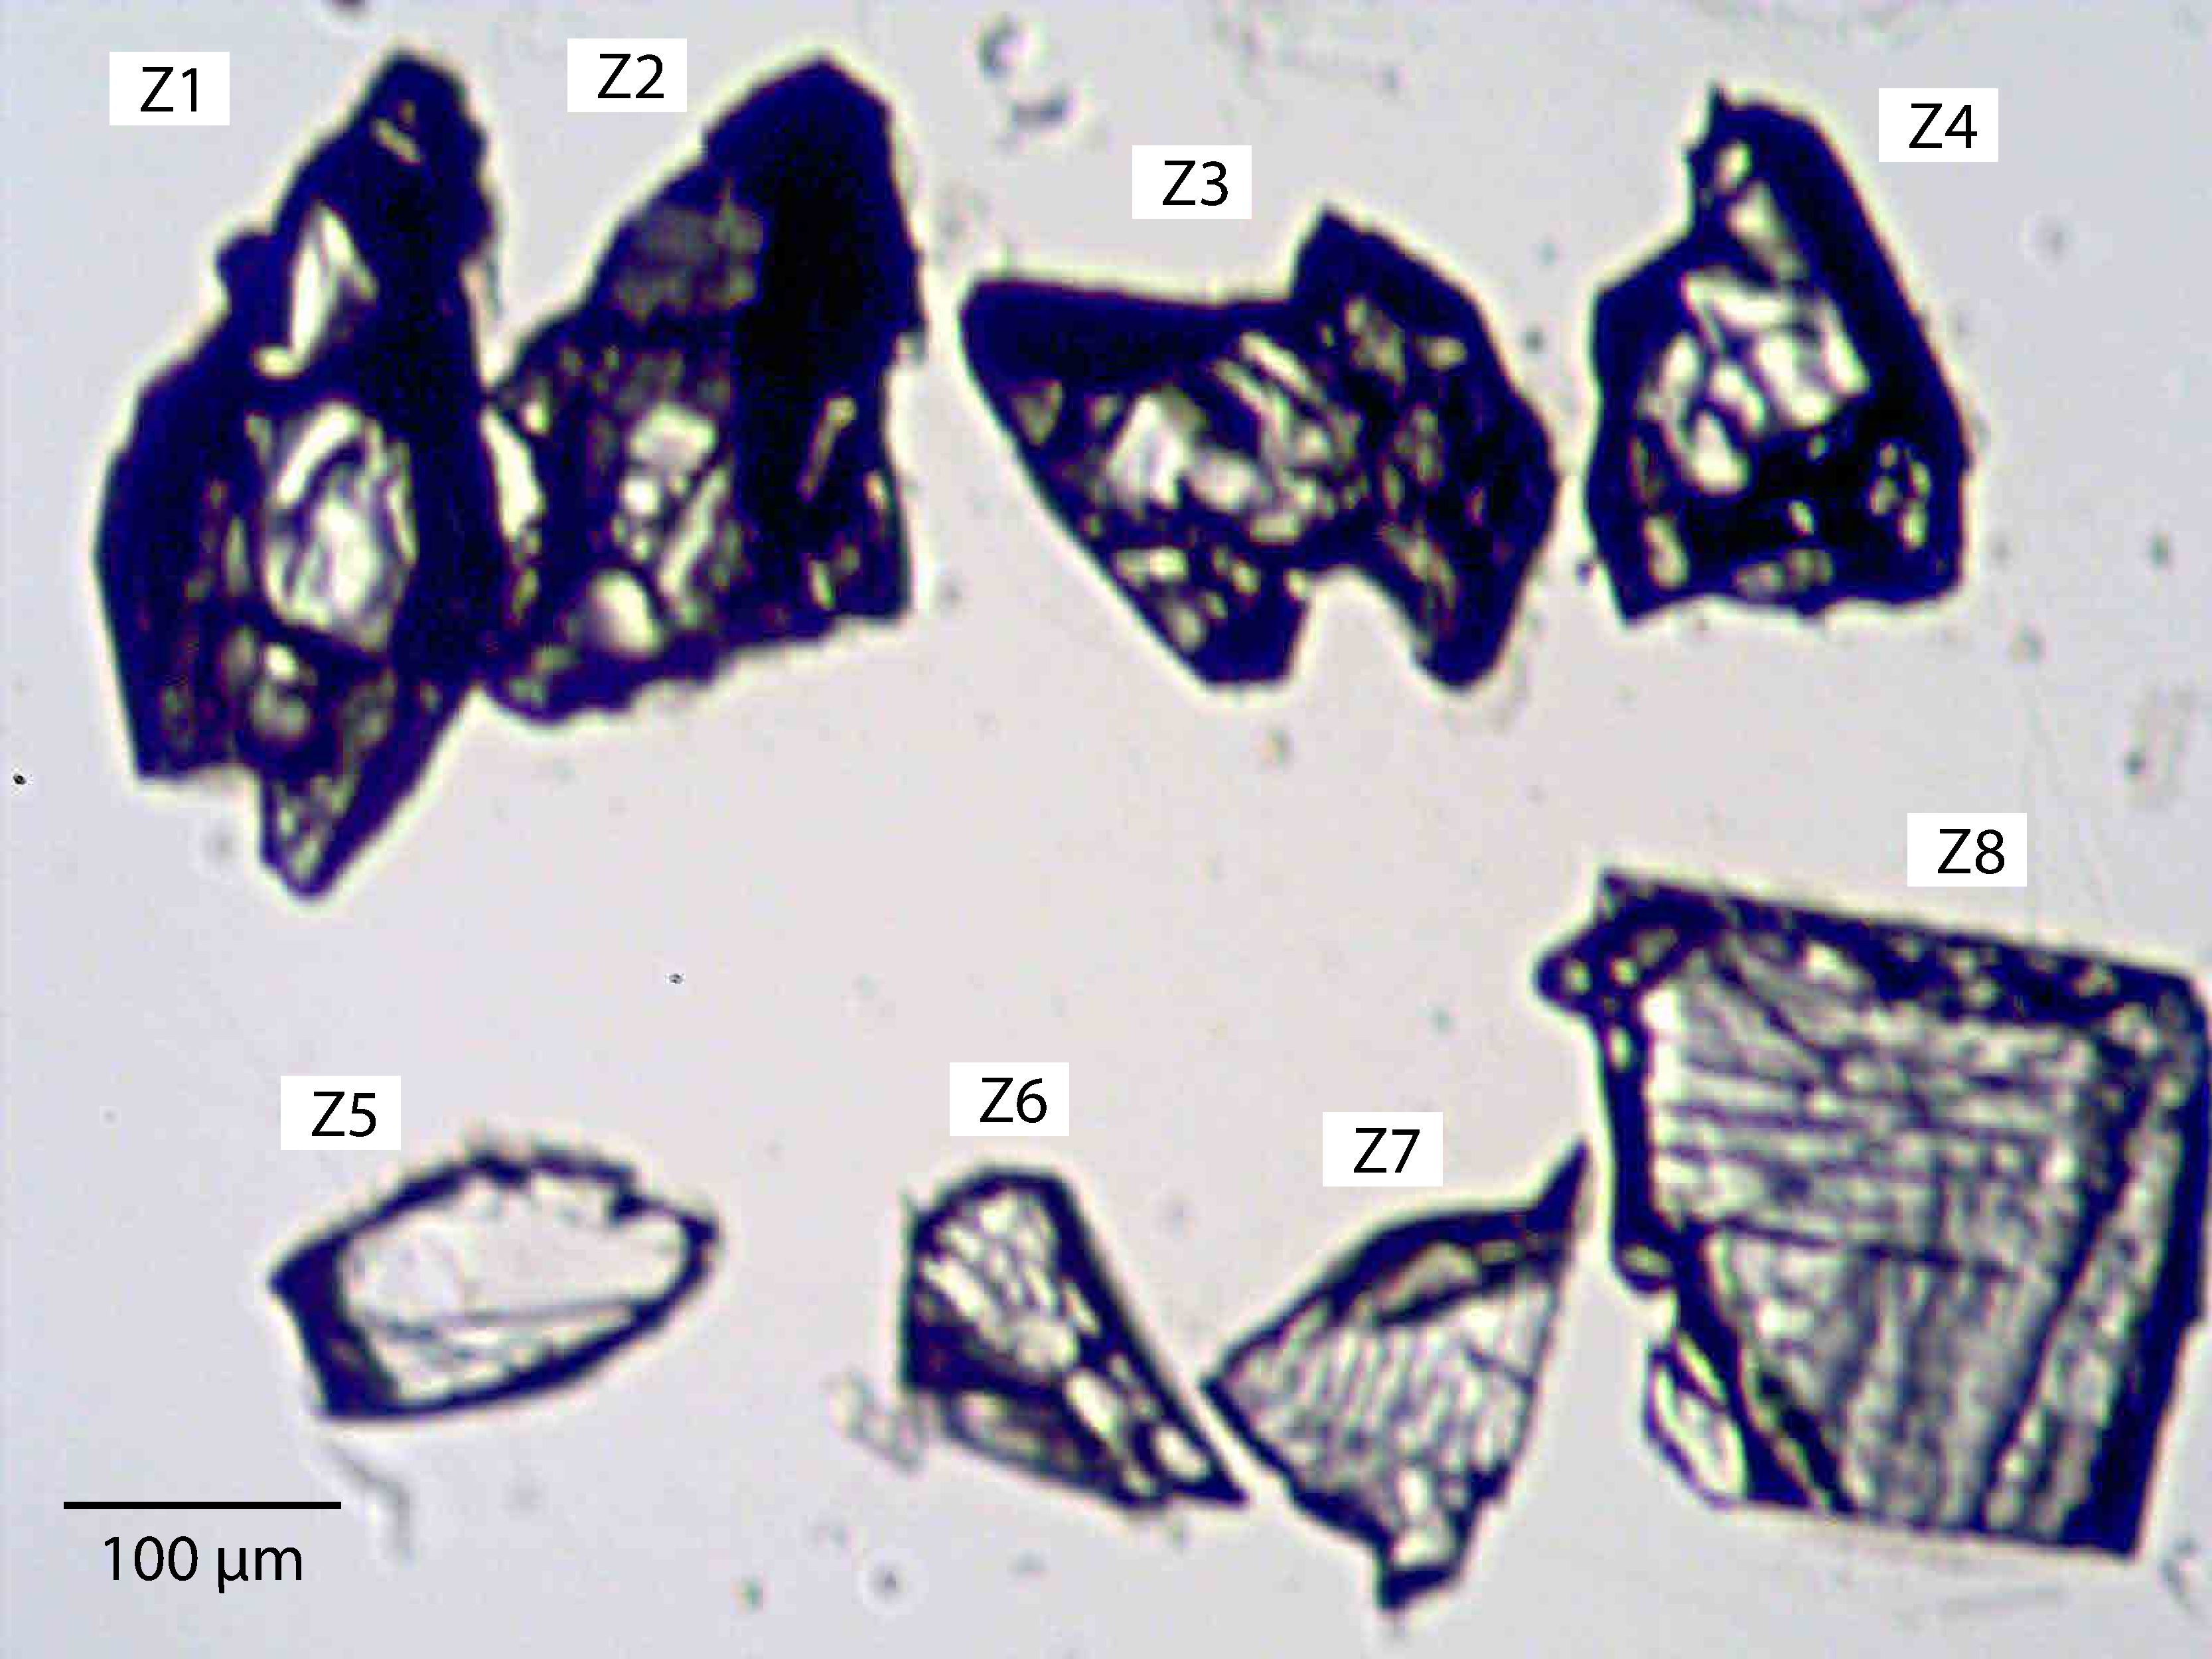
\includegraphics[width=0.9\textwidth]{figure/Zhang2021/SI_zircons.pdf}
\centering
\caption[Image of individual zircons used for ID-TIMS U-Pb geochronology from sample MS99033]{\footnotesize{Image of individual zircons used for ID-TIMS U-Pb geochronology from sample MS99033. Zircons (z1-z4) are subhedral to anhedral crystals and (z5-z8) are platy fragments.}}
\label{fig:zircon_image}
\end{figure}

\begin{figure}[h!]
\noindent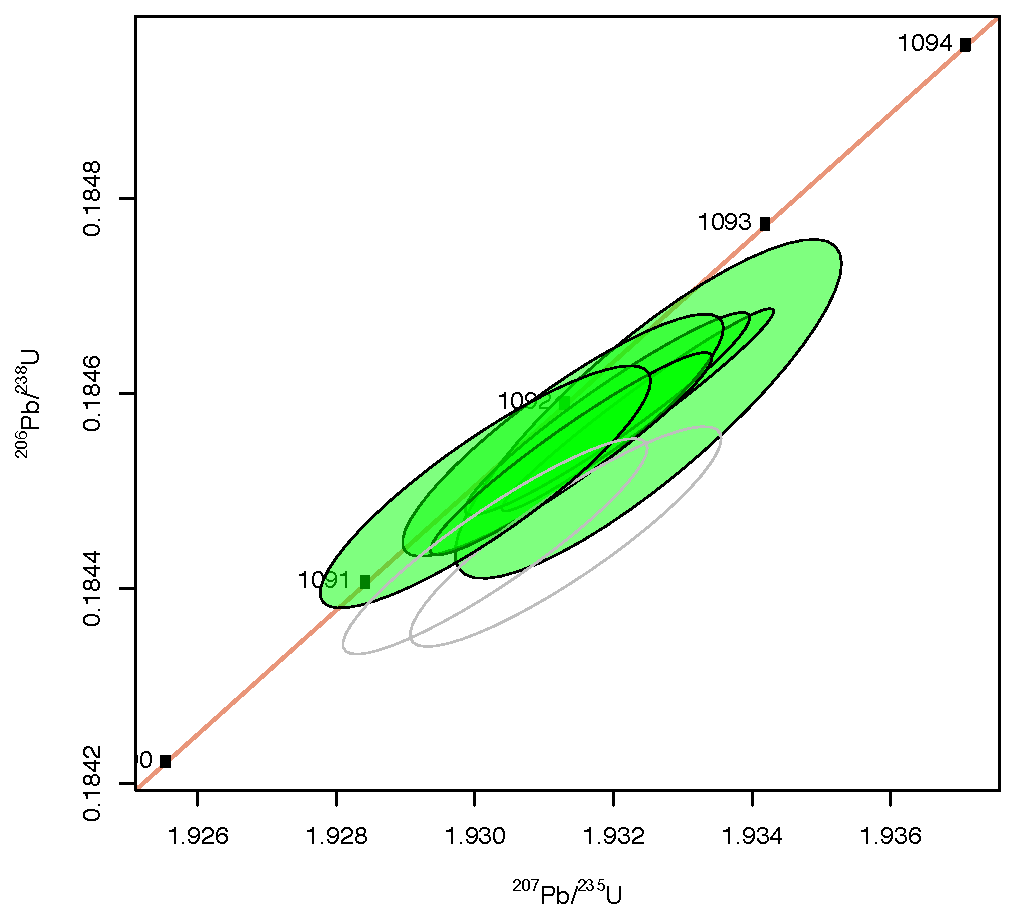
\includegraphics[width=0.8\textwidth]{figure/Zhang2021/SI_MS99033_geochron_plot.pdf}
\centering
\caption[U-Pb concordia plots for the new zircon dates from anorthosite xenoliths AX16, geochronology sample MS99033]{\footnotesize{U-Pb concordia plots for the new zircon dates from anorthosite xenoliths AX16, geochronology sample MS99033. The ellipses represent 2$\sigma$ analytical uncertainty on individual zircon dates. Green filled ellipses are analyses included in the $^{206}$Pb/$^{238}$U weighted mean dates while the grey ellipses are those that were excluded. }}
\label{fig:zircon_concordia}
\end{figure}

U-Pb dates were obtained by chemical abrasion isotope dilution thermal ionization mass spectrometry (ID-TIMS) in the Boise State University (BSU) Isotope Geology Laboratory (Table S2; Fig. \ref{fig:zircon_image}). 

Zircons were separated from the bulk rock sample using a sledge, Retsch DM200 disc mill, 500 µm sieve, Wilfley Shaker Table, LB-1 Frantz magnetic separator, and methylene iodide heavy liquid. Heavy separates were annealed at 900\textdegree C for 48 to 60 hours in quartz crucibles in a muffle furnace. Individual zircons were chemically abraded. Chemical abrasion was carried out by transferring zircons to 3 ml Teflon Perfluoroalkoxy alkane (PFA) beakers in which they were rinsed in 3.5 M HNO$_\mathrm{3}$ and ultrapure H$_\mathrm{2}$O prior to loading into 300 $\mu$l Teflon PFA microcapsules. Fifteen microcapsules were placed in a large-capacity Parr vessel and the zircon partially dissolved in 120 $\mu$l of 29 M HF for 12 hours at 190\textdegree C. Zircons were returned to 3 ml Teflon PFA beakers, HF was removed, and zircons were immersed in 3.5 M HNO$_\mathrm{3}$, ultrasonically cleaned for an hour, and fluxed on a hotplate at 80°C for an hour. The HNO$_\mathrm{3}$ was removed and zircon was rinsed twice in ultrapure H2O before being reloaded into the 300 $\mu$l Teflon PFA microcapsules (rinsed and fluxed in 6 M HCl during sonication and washing of the zircons) and spiked with the $^{233}$U-$^{235}$U-$^{205}$Pb BSU tracer solution (BSU1B). Zircons were dissolved in Parr vessels in 120 $\mu$l of 29 M HF at 220\textdegree C for 48 hours, dried to fluorides, and re-dissolved in 6 M HCl at 180\textdegree C overnight. Pb and U were separated from the zircon matrix using an HCl-based anion-exchange chromatographic procedure \citep{Krogh1973a}, eluted together and dried with 2 $\mu$l of 0.05 N H$_\mathrm{3}$PO$_\mathrm{4}$.

Pb and U were loaded on a single outgassed Re filament in 5 $\mu$l of a silica-gel/phosphoric acid mixture \citep{Gerstenberger1997a}, and Pb and U isotopic measurements made on a GV Isoprobe-T multicollector thermal ionization mass spectrometer equipped with an ion-counting Daly detector. Pb isotopes were measured by peak-jumping all isotopes on the Daly detector for 190 cycles with a mass bias correction of 0.16 $\pm$ 0.03$\%$/a.m.u. (1$\sigma$). Transitory isobaric interferences due to high-molecular weight organics, particularly on $^{204}$Pb and $^{207}$Pb, disappeared within 30-45 cycles, while ionization efficiency averaged 104 cps/pg of each Pb isotope. Linearity (to $\geq$1.4 x 10$^6$ cps) and the associated deadtime correction of the Daly detector were determined by analysis of NBS982. Uranium was analyzed as UO$_2^+$ ions in static Faraday mode on 10$^{12}$ ohm resistors for up to 300 cycles, and corrected for isobaric interference of $^{233}$U$^{18}$O$^{16}$O on $^{235}$U$^{16}$O$^{16}$O with an $^{18}$O/$^{16}$O of 0.00206. Ionization efficiency averaged 20 mV/ng of each U isotope. U mass fractionation was corrected using the $^{233}$U/$^{235}$U ratio of the BSU1B tracer. 

\section*{LA-ICPMS plagioclase geochemistry}

Rare earth elements (REE) ICPMS analyses are done by the GeoAnalytical Lab at Washington State University. Four plagioclase crystals with minimal visible other mineral inclusions from anorthosite sample MS99033 were picked for REE analyses (Table S3). The Flux used for the fusion is di-Lithium-tetraborate (Spectromelt$^@$ A-10, EM Science, Gibbstown, NJ). Reagents are HNO$_3$ 69-70\% (Fisher ACS plus grade), HF 48-52\% (Baker ACS reagent grade), HClO$_4$ 67-71\% (Fisher Trace Metal Grade), and H$_2$O$_2$ (Baker ACS Reagent). The HF is further purified before use by sub-boiling distillation in a Teflon still.  All water used is $>$18 M deionized water from a Nanopure analytical grade water system (Barnstead/Thermolyne)

Powdered samples are mixed with an equal amount of lithium tetraborate flux (typically 2g), placed in a carbon crucible and fused at 1000\textdegree C in a muffle furnace for 30 minutes. After cooling, the resultant fusion bead is briefly ground in a carbon-steel ring mill and a 250 mg portion is weighed into a 30 ml, screw-top Teflon PFA vial for dissolution. The acid dissolution consists of a first evaporation with HNO$_3$ (2ml), HF (6 ml), and HClO$_4$ (2 ml) at 110\textdegree C. After evaporating to dryness, the sample is wetted and the sides of the vial are rinsed with a small amount of water before a second evaporation with HClO$_4$ (2 ml) at 160\textdegree C. After the second evaporation, samples are brought into solution by adding approximately 10 ml of water, 3 ml HNO$_3$, 5 drops H$_2$O$_2$, 2 drops of HF and warmed on a hot plate until a clear solution is obtained. The sample is then transferred to a clean 60 ml HDPE bottle diluted up to a final weight of 60g with deionized water.

Solutions are analyzed on an Agilent model 4500 ICPMS and are diluted an additional 10X at the time of analysis using Agilent’s Integrated Sample Introduction System (ISIS). This yields a final dilution factor of 1:4800 relative to the amount of sample fused. Instrumental drift is corrected using Ru, In, and Re as internal standards. Internal standardization for the REEs uses a linear interpolation between In and Re after \cite{Doherty1989a} to compensate for mass-dependant differences in the rate and degree of instrumental drift. Isobaric interference of light rare earth oxides on the mid- heavy REEs can be a significant source of error in ICPMS analysis, so tuning is optimized to keep the CeO/Ce ratio below 0.5\%. Correction factors used to compensate for the remaining oxide interferences are estimated using two mixed-element solutions. The first contains Ba, Pr, and Nd, and the second Tb, Sm, Eu, and Gd.  Standardization is accomplished by processing duplicates of three in-house rock standards interspersed within each batch of 18 unknowns. Concentrations, oxide- and drift corrections are then calculated offline using a spreadsheet. Methods description is provided by: \url{https://environment.wsu.edu/facilities/geoanalytical-lab/technical-notes/icp-ms-method/}.  


\section*{LA-ICPMS zircon geochemistry}

15 zircons extracted from sample MS99033 were analyzed by laser ablation inductively coupled plasma mass spectrometry (LA-ICPMS) using a ThermoElectron, iCAP-RQ, single quadrupole ICPMS and a Teledyne (Photon Machines) Analyte Excite+ 193 nm excimer Analyte laser with a HelEx ablation cell at BSU. Analytical protocols, standard materials, and data reduction software developed at BSU were used for acquisition and calibration of U-Pb dates and a suite of high field strength elements (HFSE) and rare earth elements (REE). Zircon were ablated with a 25 µm diameter laser spot using fluence and pulse rates of $\sim$2.5 J/cm2 and $\sim$5 Hz, respectively, during a 20-second analysis excavating a pit 25 µm deep. Ablated material was carried to the nebulizer flow of the plasma by a 1.2 L/min He gas stream. Total sweep duration is 895 ms, and quadrupole dwell times were 5 ms for Si and Zr, 40 ms for $^{202}$Hg, $^{204}$Pb, $^{208}$Pb, $^{232}$Th, and $^{238}$U, 80 ms for $^{206}$Pb, 200 ms for $^{49}$Ti and $^{207}$Pb, and 10 ms for all other HFSE and REE. Background count rates were obtained prior to each spot analysis and subtracted from the raw count rate for each analyte. Concentrations were calculated using background-subtracted count rates internally normalized to $^{29}$Si and calibrated with the primary standards NIST SRM-610 and -612 glasses. Ablation pits that intersected mineral inclusions were identified based on Ti and P spikes. The Ti-in-zircon thermometer was calculated using an average TiO$_2$ activity value of 0.7 in crustal rocks \citep{Watson2006a} and an average SiO$_2$ activity value of 1.0 \citep{Ferry2007a}. 

\section*{Additional zircon photomicrograph}
\begin{figure}[h!]
\noindent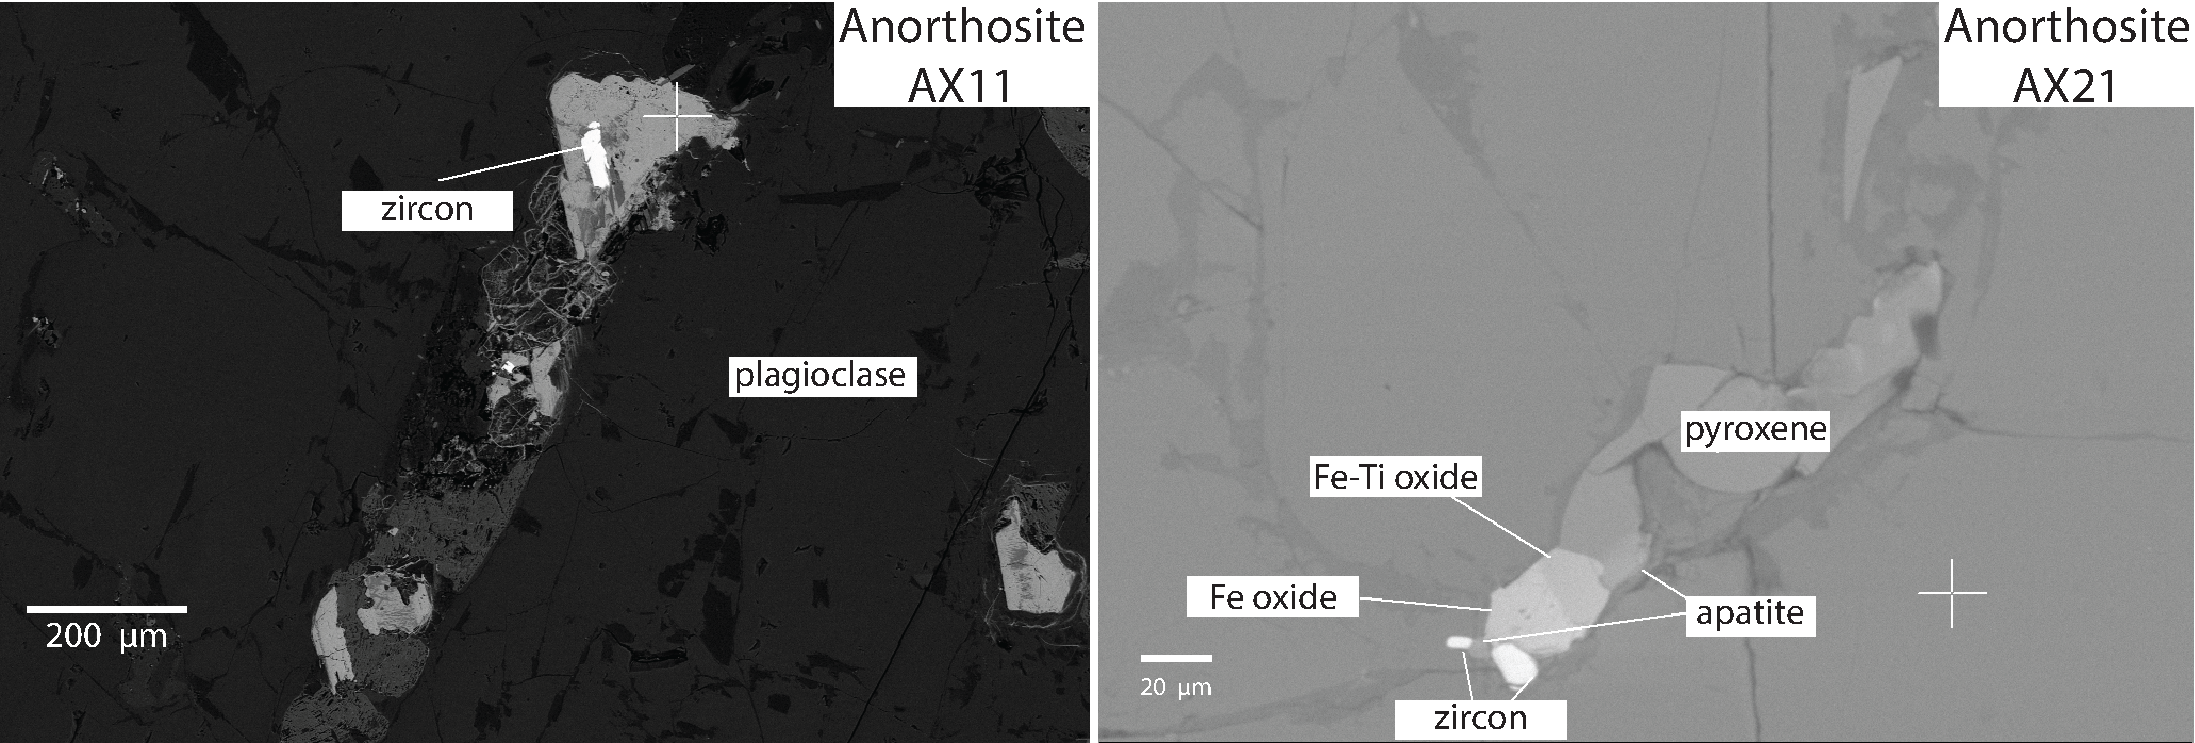
\includegraphics[width=\textwidth]{figure/Zhang2021/SI_interstitial_zircons.pdf}
\caption[Backscattered electron (BSE) images of anorthosite xenoliths.]{\footnotesize{Backscattered electron (BSE) images of anorthosite xenoliths. Subhedral to anhedral zircons form next to mafic melt pockets.}}
\label{fig:interstitial_zircons}
\end{figure}

Fig. \ref{fig:interstitial_zircons} shows subhedral and anhedral zircons in anorthosite xenoliths AX11 and AX21 in back scattered electron (BSE) images of anorthosite thin sections. All zircons found are interstitial to the plagioclase. This texture is consistent with the interpretation of a zircon formation from interstitial melt liquids preserved in plagioclase mush.

\section*{Beaver River diabase structural correction}

Structural measurements were obtained from the published geologic maps of the study area as well as our field data. We calculated the mean directions from the combined volcanic bedding measurements from the Schroeder-Lutsen basalt and igneous layering measurements from the Beaver River diabase and constructed two sets of tilt correction data for the paleomagnetic sites in the southern and eastern Beaver Bay Complex \citep{Boerboom2004a, Boerboom2006a, Boerboom2006b, Boerboom2007a, Miller2001a}. The mean dip angle for the two areas are very similar while the dip trends are different, with the southern Beaver Bay Complex showing a slightly more easterly trend than the eastern Beaver Bay Complex. This difference in dip trend reflects the overall arcuate shape of the Beaver Bay Complex intrusions along the shore of Lake Superior. 

\begin{figure}[h!]
\noindent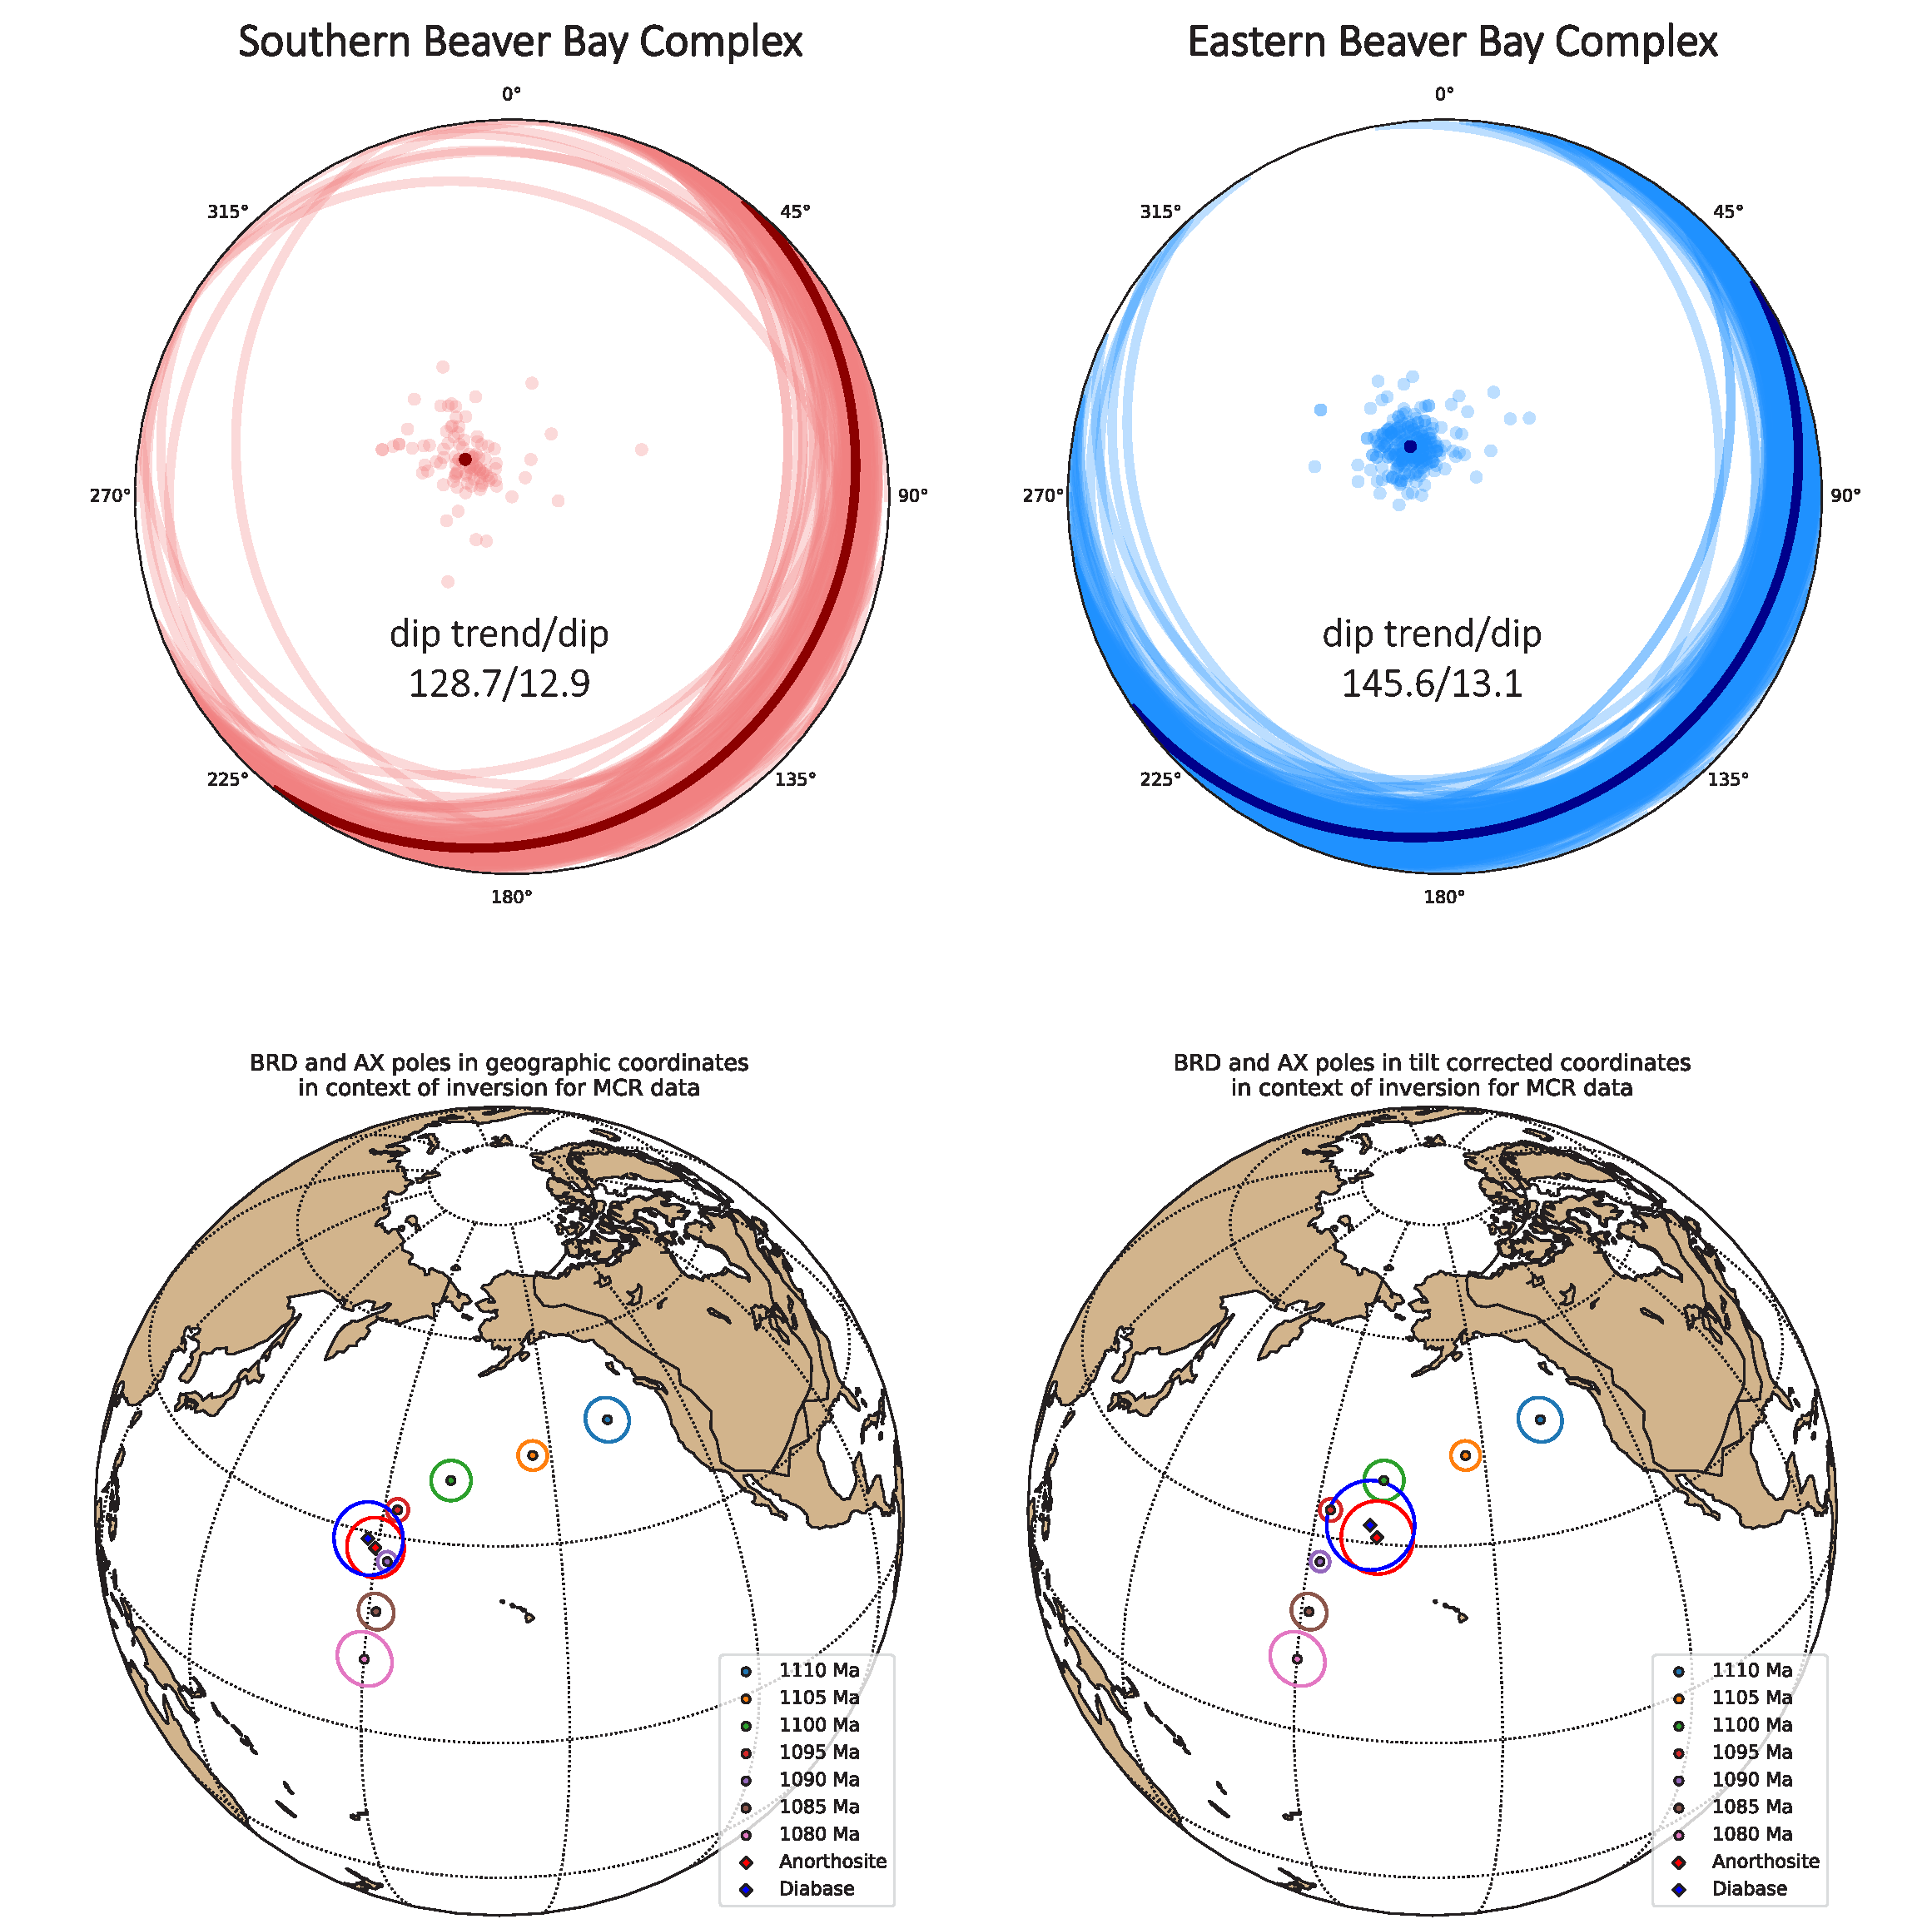
\includegraphics[width=0.9\textwidth]{figure/Zhang2021/SI_tilt_correction.pdf}
\centering
\caption[Tilt correction analyses for the Beaver River diabase and anorthosite paleomagnetic data]{\footnotesize{Stereonet plots of the compiled structural orientation data to tilt correct the paleomagnetic directions obtained from the Beaver River diabase and the anorthosite xenoliths therein. The mean pole position of the diabase and anorthosite units before and after the tilt correction are shown in context of the inverted Keweenawan Track developed by \cite{Swanson-Hysell2019a}.}}
\label{fig:tilt_correction}
\end{figure}

To summarize, We use a bedding dip direction - dip of 145.6 - 13.1 for paleomagnetic site AX3, AX4, AX5, AX6, AX7, AX8, AX9, AX10, and BD2, BD14, BD15, BD16 in the Eastern Beaver Bay Complex region. We use a bedding dip direction - dip of 128.7 - 12.9 for site AX1, AX2, AX11, AX12, AX13, AX14, AX15, AX16, AX17, AX18, AX19, AX20, AX21, AX22, BD1, BD3, BD4, BD5, BD6, BD7. BD8. BD9, BD10, BD11, BD12, BD13, BD17 in the Southern Beaver Bay Complex.

Fig. \ref{fig:tilt_correction} shows the stereonet plots of the bedding orientations compiled for tilt correcting the paleomagnetic directions of samples collected in the Southern Beaver Bay Complex and the Eastern Beaver Bay Complex. The resultant mean pole position for the diabase changes from 29.0\textdegree N, 178.2\textdegree E, N = 15, A95 = 5.2\textdegree, k = 55.3 before tilt correction to 32.5\textdegree N, 189.5\textdegree E, N = 15, A95 = 6.3\textdegree, k = 37.4 after tilt correction. For the anorthosite, the mean pole position changes from 28.0\textdegree N, 179.6\textdegree E, N = 17, A95 = 4.3\textdegree, k = 70.6 before tilt correction to 30.9\textdegree N, 190.8\textdegree E, N = 17, A95: 5.2\textdegree, k = 48.5 after tilt correction. The uncertainty ellipses for both units are slightly larger after tilt correcting the directions. This may reflect the uncertainties associated with using igneous fabrics as our paleohorizontal references. Nevertheless, the mean pole position of the diabase and anorthosite still overlaps and is consistent with the expected position derived from the inverted Keweenawan Track \textit{ca.} 1092 Ma \citep{Swanson-Hysell2019a}. 


\clearpage
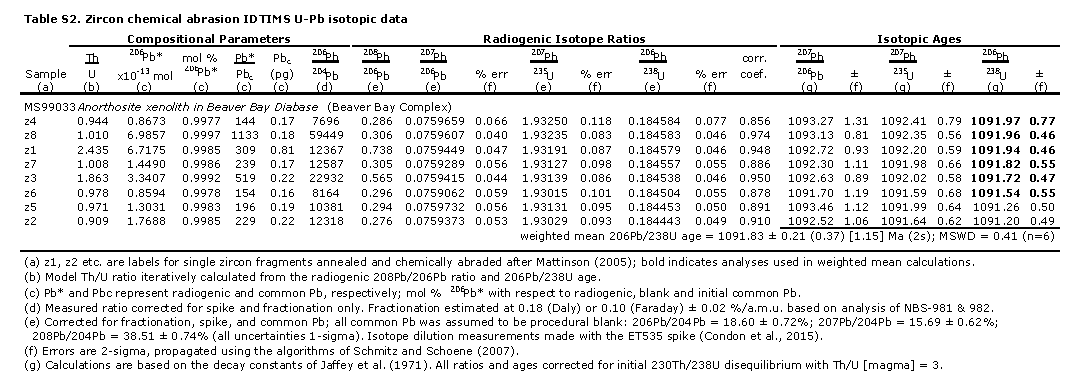
\includepdf[width=7.65 in]{figure/Zhang2021/SI_MS99033_geochron.pdf}

\clearpage
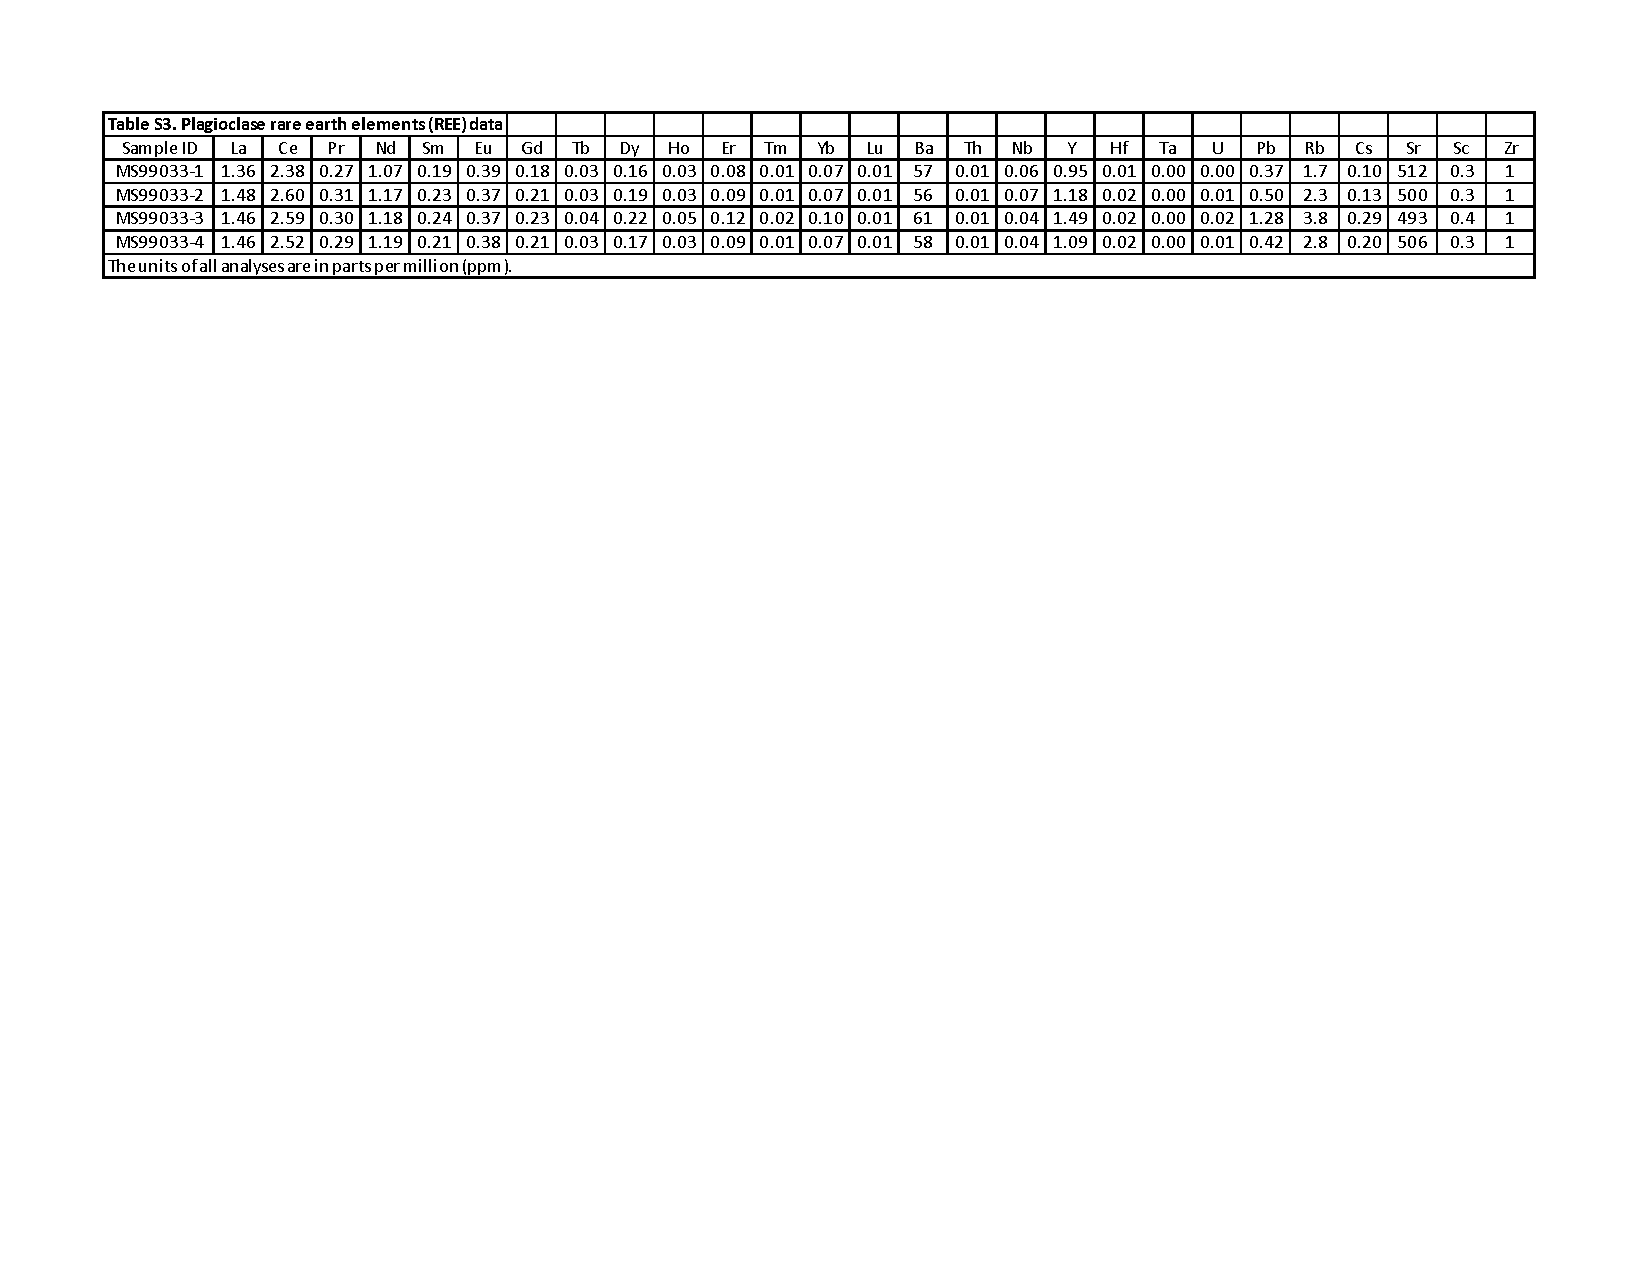
\includepdf[width=7.65 in]{figure/Zhang2021/SI_plag_REE_table.pdf}

\nocite{Mattinson2005a, Condon2015a, Schmitz2007a, Jaffe1975a}

\clearpage


\chapter[Supporting Information for ``High geomagnetic field intensity recorded by anorthosite xenoliths requires a vigorous late Mesoproterozoic geodynamo"][Supporting Information--Late Mesoproterozoic Geodynamo]{Supporting Information for ``High geomagnetic field intensity recorded by anorthosite xenoliths requires a vigorous late Mesoproterozoic geodynamo"}


\begin{figure}
\noindent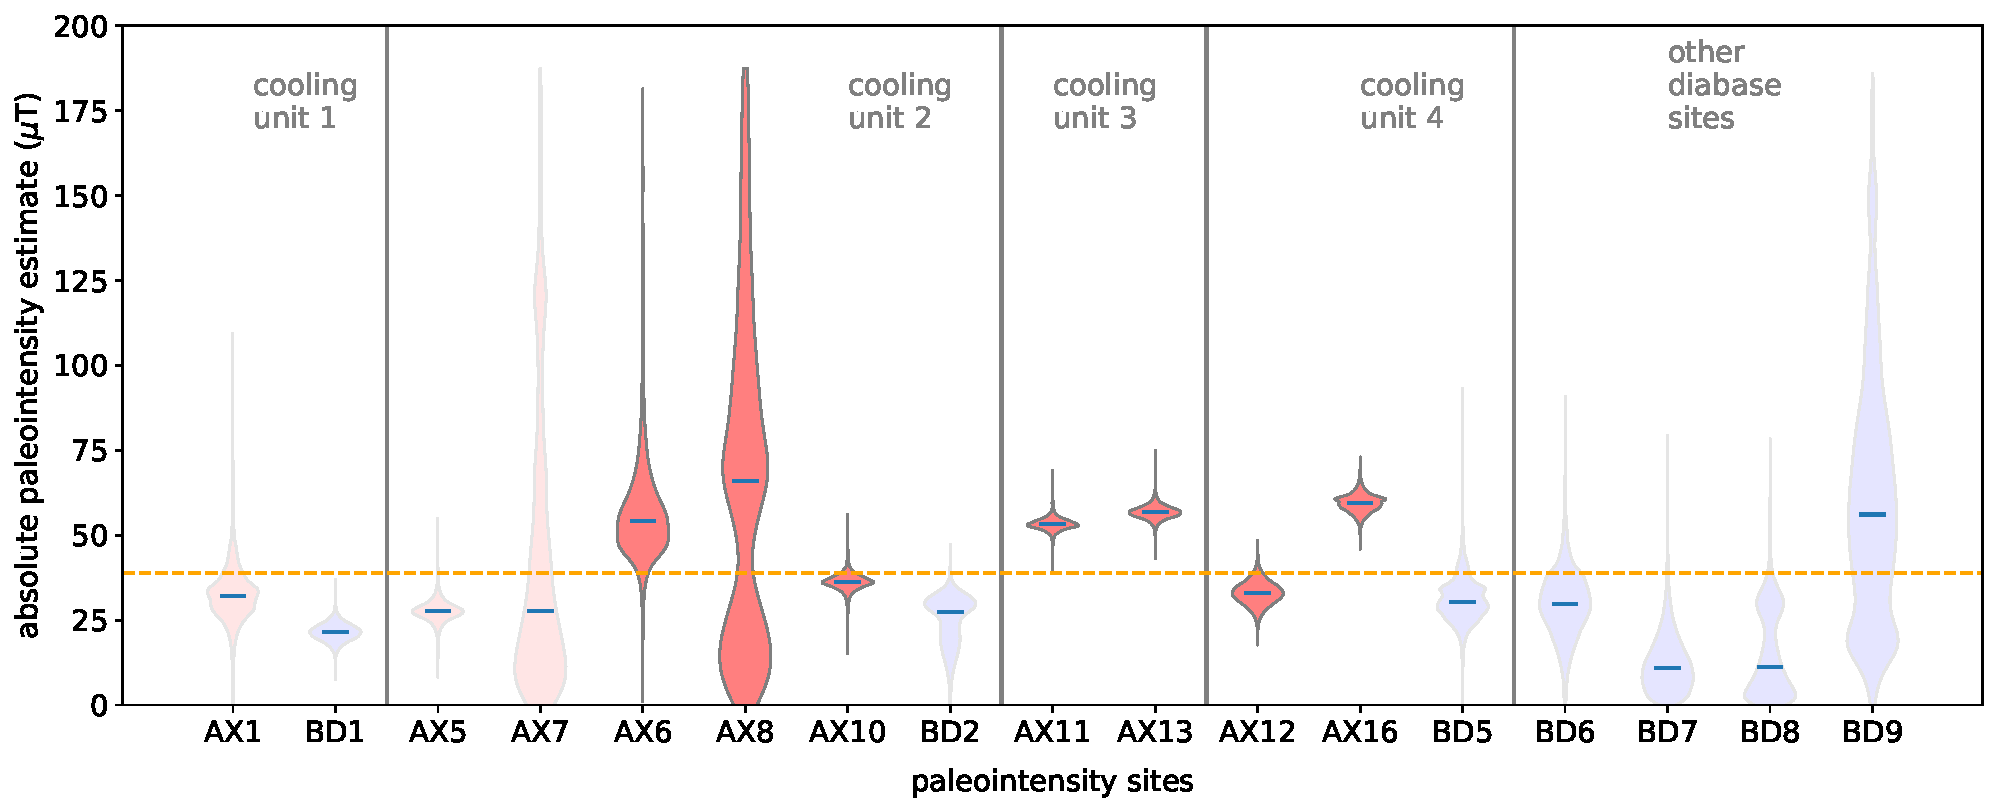
\includegraphics[width=0.9\textwidth]{figure/Zhang2022/PINT_BiCEP.pdf}
\centering
\caption[Beaver River anorthosite and diabase paleointensity estimates based on the BiCEP method]{Violin plots of site-level posterior paleointensity distributions estimated using the bias corrected estimation of paleointensity (BiCEP) method developed by ref. \citealp{Cych2021a}. Blue bars of each violin plot represent the median of the distributions. The yellow dashed line is the mean paleointensity of the posterior estimates across all sites estimated using BiCEP (38.82 $\pm$ 4.60 mT). Assuming that paleointensity estimates from specimens that come from a same cooling unit are distributed around a true paleointensity value with the various deflections being expressed as the curvature parameter of the NRM/TRM plot \cite{Arai1963a, Paterson2011a}, the method uses all paleointensity measurement-level data without applying selection criteria. For comparison of results from this independent method with those based on our selection (as show in Fig. 4 in manuscript), we highlight the anorthosite sites that pass our paleointensity selection and make other anorthosite and diabase more transparent. The results from the BiCEP method address the uncertainties associated with anorthosite AX6 and AX8. This is associated with the relatively variable specimen behaviors within these two sites. For sites AX10, AX11, AX13, AX12, and AX16, the posterior probability distributions have very narrow bounds, consistent with the interpretation that these anorthosites are faithful paleointensity recorders that have high-quality paleointensity behaviors. AX--anorthosite xenolith site; BD--Beaver River diabase site. The grouping of cooling units is based on the spatial proximity between site locations and the inclusion relationship of host diabase and anorthosite xenoliths reported by ref. \citealp{Zhang2021b}.}
\label{fig:PINT_BiCEP}
\end{figure}

\clearpage

\begin{figure}
\noindent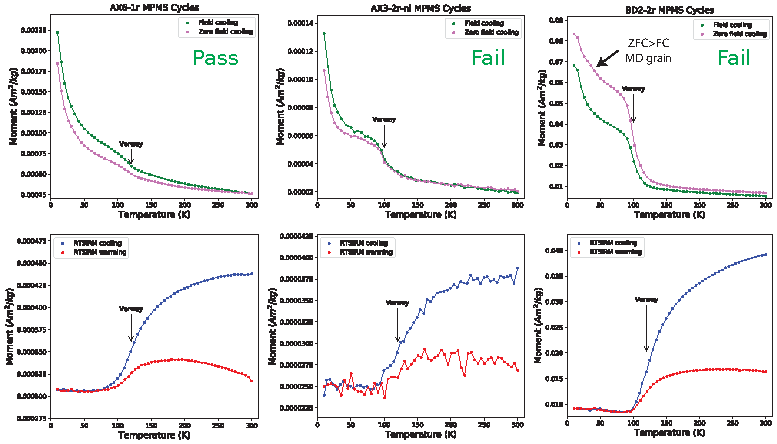
\includegraphics[width=0.9\textwidth]{figure/Zhang2022/MPMS.pdf}
\centering
\caption[Beaver River diabase and anorthosite low-temperature magnetic property measurement results]{Low-temperature magnetic property measurement system (MPMS) experiment results. ``Pass" or ``Fail" represents whether their sister specimens passed our paleointensity selection or not. In the field-cooled (FC) experiments, the magnetization was measured upon warming following the specimen having cooled in an applied field of 2.5 T from 300 to 10 K. In the zero-field-cooled (ZFC) experiment, a low-temperature saturation isothermal remanence (LTSIRM) of 2.5 T was applied at 10 K after the specimen cooled in a (near-)zero field. In the room-temperature saturation isothermal remanence (RTSIRM) experiment, the sample was pulsed with a 2.5 T field at room temperature ($\sim$300 K) and then cooled to 10 K and warmed back to room temperature in a (near-) zero field. Specimen AX6-1r is from anorthosite AX6 which passed our paleointensity selection. It has a well-defined Verwey transition $\sim$120 K \cite{Verwey1939a}. Specimens AX3-2r-ni and BD2-2r show Verwey transition but the transition temperatures are suppressed below $\sim$120 K. Specimen BD2-2r has a consistently higher moment during the zero-field-cooled step than during the field-cooled step. This is consistent with the interpretation that multidomain (MD) magnetic carriers exist in significant quantity in this specimen \cite{Carter-Stiglitz2006a}.}
\label{fig:MPMS}
\end{figure}

\clearpage

\begin{figure}
\noindent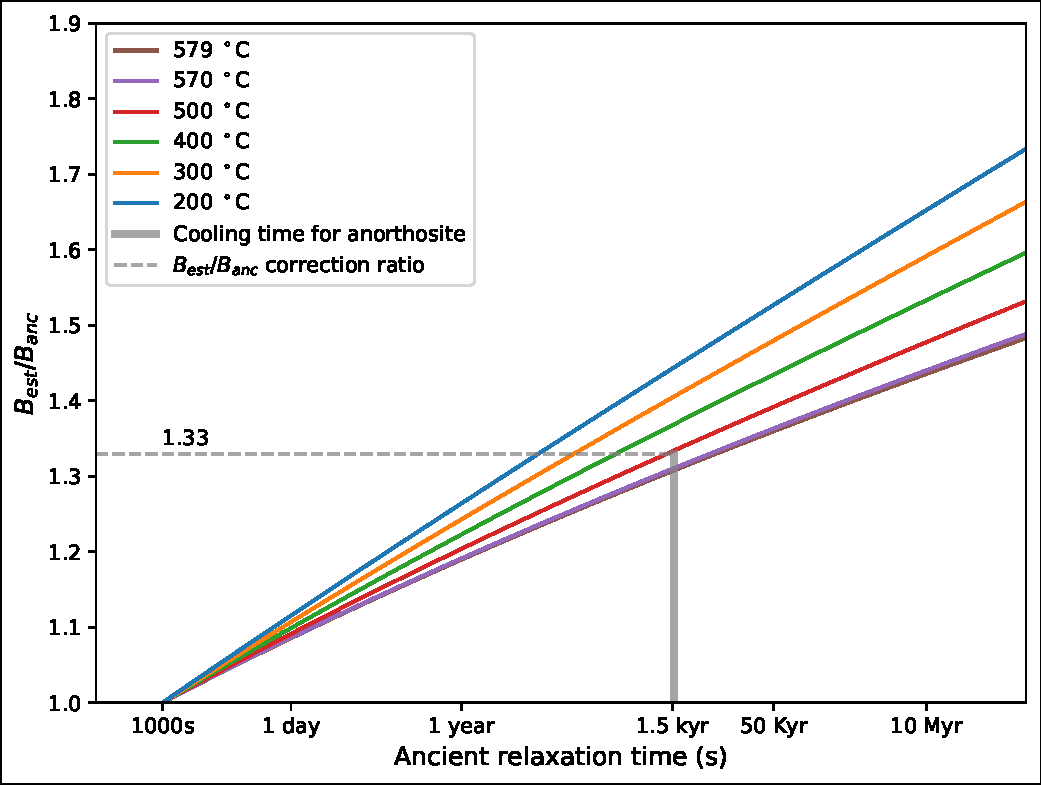
\includegraphics[width=0.9\textwidth]{figure/Zhang2022/Cooling_rate_correction.pdf}
\centering
\caption[Beaver River anorthosite cooling rate correction for paleointensity estimates]{Graph of predicted paleointensity overestimate due to slow cooling of the intrusive Beaver River diabase and anorthosite xenoliths relative to the cooling rate in laboratory following the model of ref. \citealp{Halgedahl1980a}. Because the majority of the anorthosites have unblocking temperatures between 500\textdegree C and 580\textdegree C, we estimate that the slow cooling during natural remanence acquisition could have resulted in a 33\% overestimate. Thus, a correction factor of 0.75 is applied at specimen level for the paleointensity summary plot.}
\label{fig:SI_PINT_cooling_corrected}
\end{figure}

\clearpage


\begin{figure}
\noindent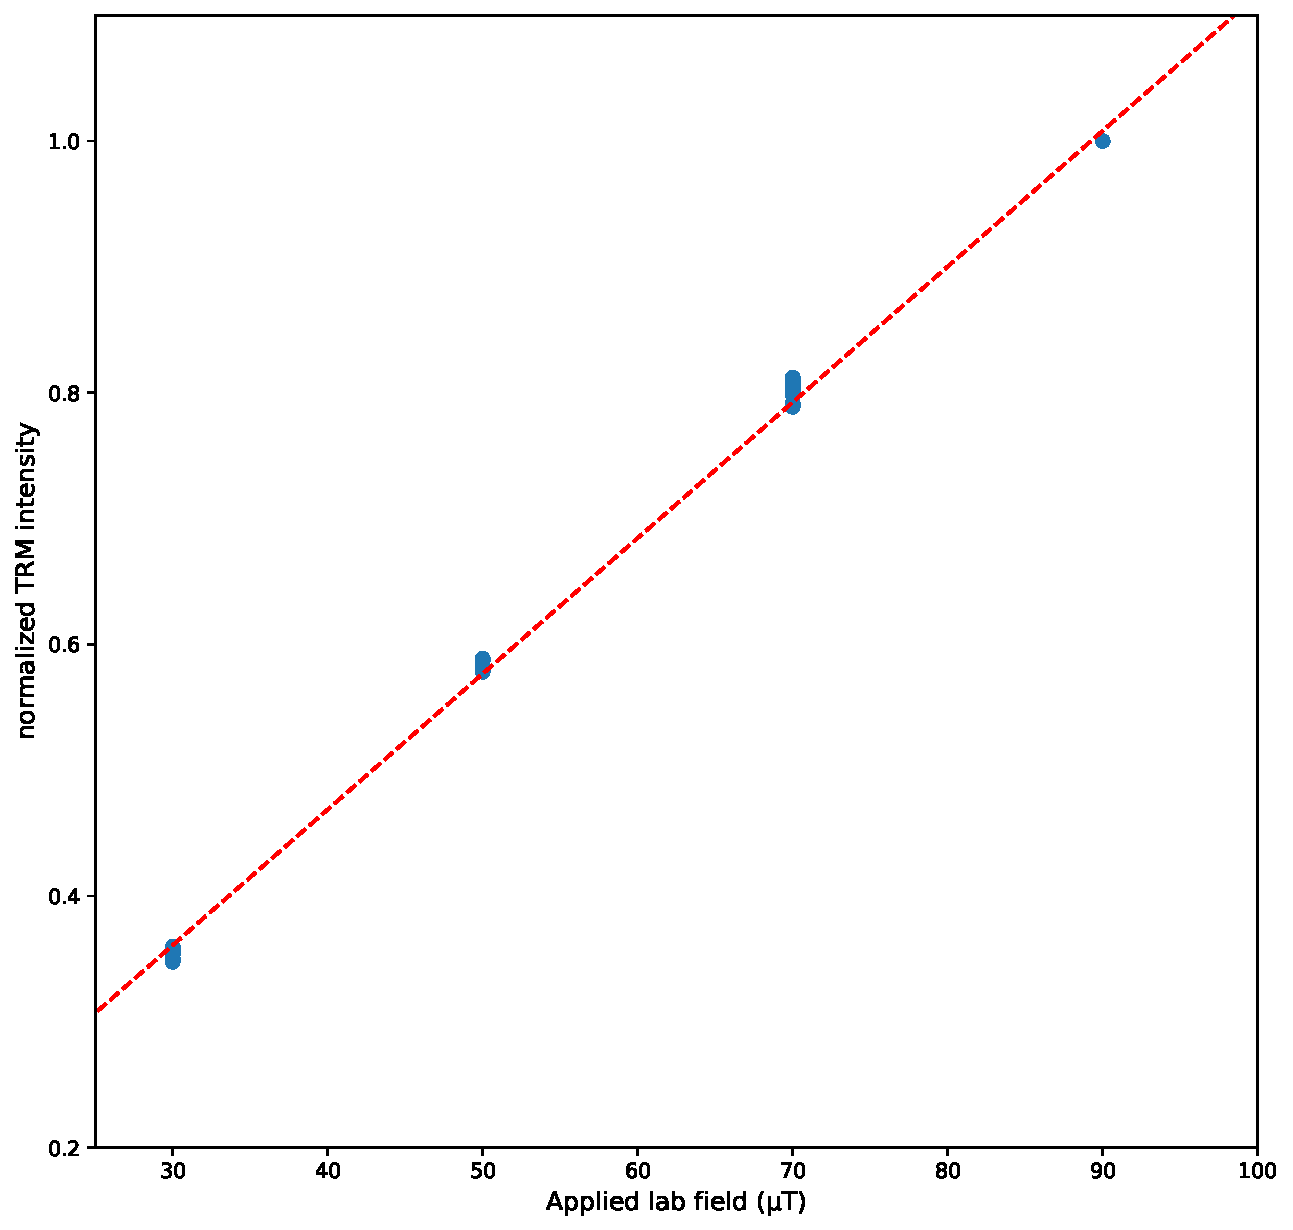
\includegraphics[width=0.9\textwidth]{figure/Zhang2022/Linear_TRM_test.pdf}
\centering
\caption[Plot of thermal remanent magnetization acquisition experiment results]{Plot of thermal remanent magnetization acquisition experiment results. After IZZI-type Thellier paleointensity experiments, full TRMs were imparted on the same specimens in known lab fields of 30, 50, 70, and 90 $\mu$T. The red dashed line shows a linear fit through the data points. The results show that the anorthosite xenoliths do not acquire saturation remanence or display non-linear remanence acquisition under fields relevant to this study. Therefore, non-linear acquisition correction is not needed for our paleointensity results. }
\label{fig:nonlinear_check}
\end{figure}

\clearpage

\begin{figure}
\noindent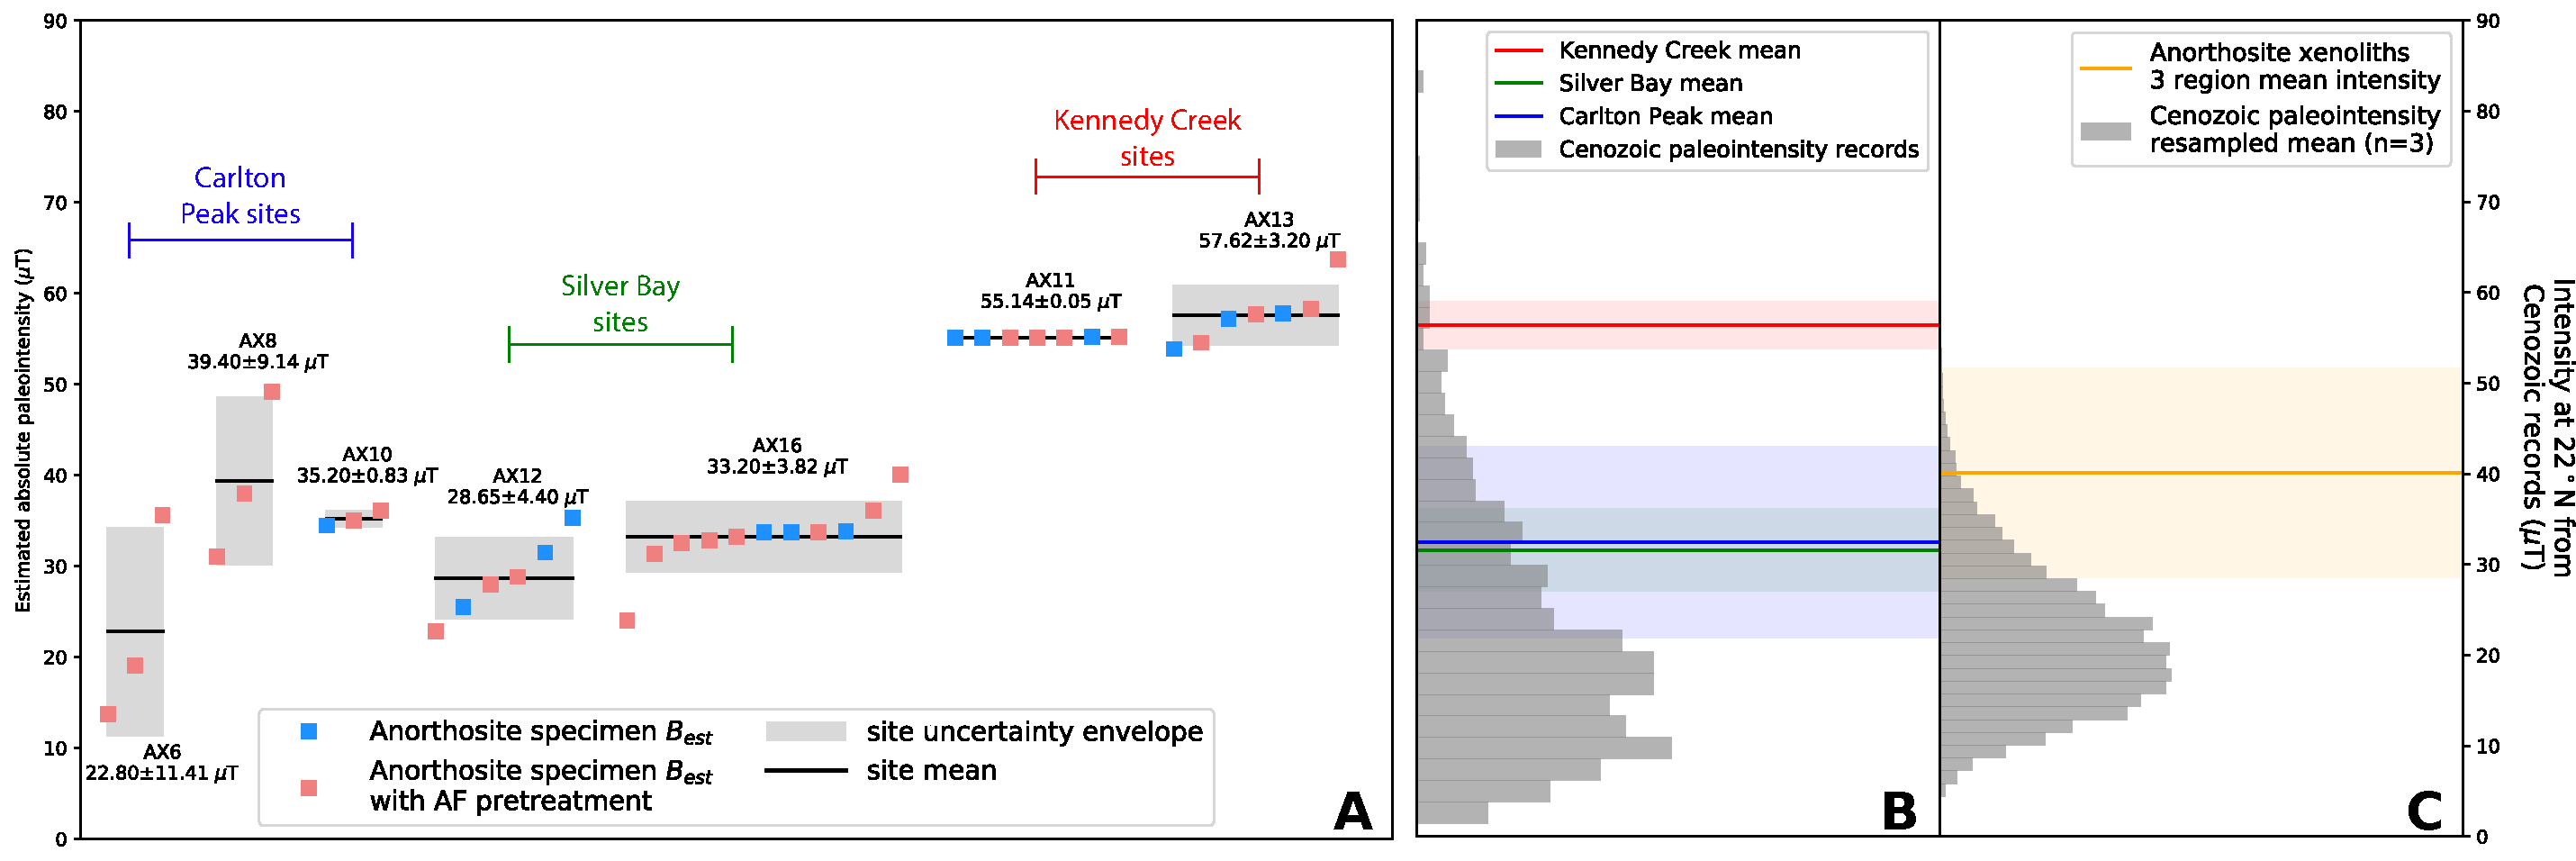
\includegraphics[width=\textwidth]{figure/Zhang2022/Cenozoic_resample_SI.pdf}
\centering
\caption[Comparison between Beaver River anorthosite paleointensity results and compilation of the Cenozoic database]{\footnotesize{Data from this study as in Figure 4 of the main text, but compared to the Cenozoic paleointensity database rather than the PADM2M model. A) Summary plot of individual specimen absolute paleointensity results (square symbols) and their averages and standard deviations at site level (black bars with grey uncertainty boxes) from this study. All results are corrected for cooling rate with a factor of 0.75. Each `AX' site is an individual anorthosite xenolith within the Beaver River diabase. The sites with successful experiments come from 3 regions which would have cooled at distinct times yielding similar estimates within the each region with differences between regions. B) Specimen level means calculated for these regions are compared to the distribution of intensities calculated from the existing paleointensity data in the Cenozoic (past 66 Myr) in the PINT database (PINT v8.0.0; \url{http://www.pintdb.org/}; \citealp{Bono2022a}) at the latitude corresponding to the paleolatitude of study region (22\textdegree N). C) The mean of the 3 regional means is compared to means calculated from 3 random values drawn from the Cenozoic data. The paleointensity records used for resampling are filtered for Q$_{PI} \geq$3 \cite{Biggin2014a}. The distribution represents a total of 10,000 iterations of taking 3 random draws and calculating the mean.}}
\label{fig:SI_Cenozoic_PINT}
\end{figure}

\clearpage

\begin{figure}
\noindent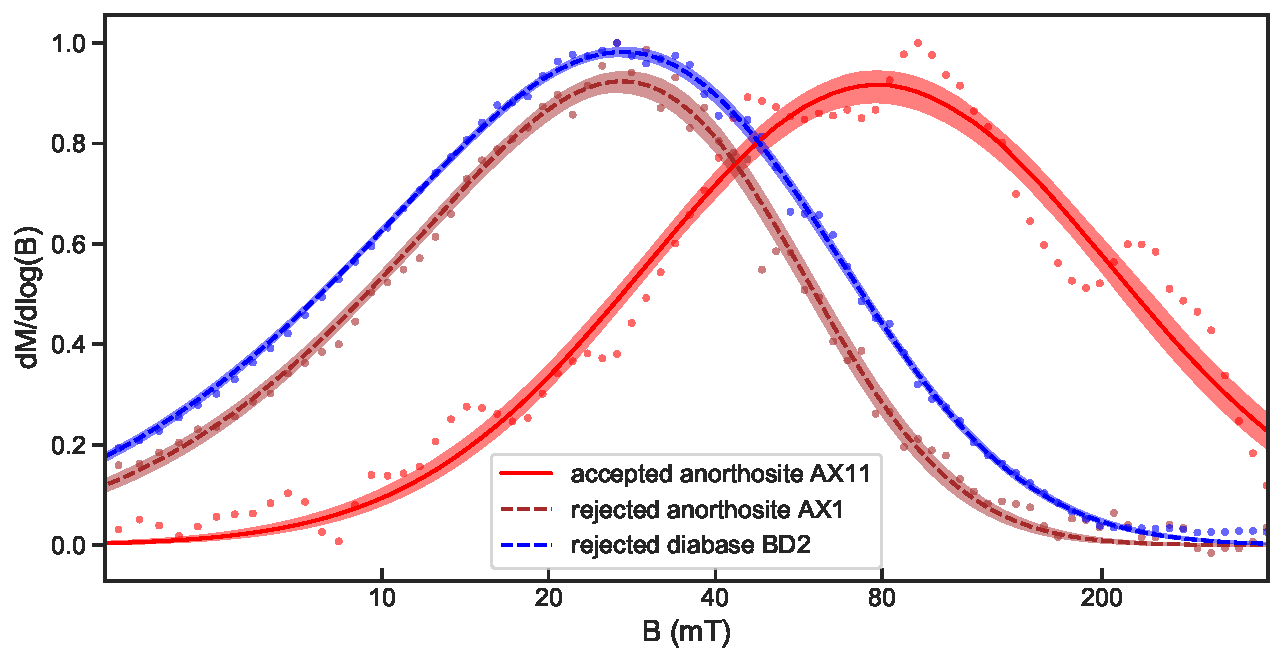
\includegraphics[width=0.9\textwidth]{figure/Zhang2022/example_unmix_plot_with_data.pdf}
\centering
\caption[Example coercivity spectra of anorthosite and diabase specimens]{\footnotesize{Example coercivity spectra of anorthosite and diabase specimens from sites that pass or fail our paleointensity selection criteria. The specimens and fits are the same as those shown in Figure 5 in the manuscript. Data points used for fitting the coercivity curves are shown in this figure. }}
\label{fig:Cenozoic_PINT}
\end{figure}

\clearpage

\begin{sidewaystable}
\tiny
\caption[Specimen paleointensity results that passed our selection]{\tiny Specimen paleointensity results that passed our selection. B$_{anc}$ is the calculated ancient field intensity over the chosen temperature interval in $\mu$T. T$_{min}$ and T$_{max}$ indicate the temperature interval over which the best fit for paleointensity was defined. N is the number of steps used within the selected interval for paleointensity determination. FRAC is the fraction of remanence used for fitting. NpTRM shows the number of pTRM checks within the selected interval for paleointensity determination. $\beta$ is the scatter parameter. GAP-MAX is the maximum magnetization gap between two adjacent steps. MAD is the maximum angle of deviation. DANG is the deviation angle. SCAT is the scatter parameter. inc$_{tc}$ is the tilt-corrected inclination. Paleolatitude is calculated from the inclination values reported in \cite{Zhang2021b}. $\gamma$ is the gamma statistic that measures the angle between the last pTRM step used for paleointensity determination and the applied field direction. V(A)DM is the virtual (axial) dipole moment reported in $10^{21}$Am$^2$ (ZAm$^2$). }
\resizebox{0.9\textwidth}{!}{\begin{tabular}{p{0.6cm}p{1.2cm}p{0.6cm}p{0.6cm}p{0.6cm}p{0.4cm}p{0.8cm} c c p{0.6cm}p{0.6cm}p{1cm}p{1cm}p{1cm} c c p {0.8cm}}
\hline
Site & Specimen & B$_{anc}$ & T$_{min}$ & T$_{max}$ & N  & FRAC & NpTRM & $\beta$ & GAP-MAX & MAD ($^\circ$) & DANG ($^\circ$) & SCAT & inc$_{tc}$ & Paleolatitude & $\gamma$ & VDM (ZAm$^2$) \\
\hline
AX6  & AX6-2a   & 13.72     & 400       & 585       & 18 & 0.70 & 10    & 0.04    & 0.12    & 3.4            & 3.4             & PASS & 38.9       & 22.0          & 2.7      & 29.8          \\
AX6  & AX6-3a   & 19.09     & 400       & 585       & 18 & 0.76 & 10    & 0.04    & 0.10    & 4.3            & 2.9             & PASS & 38.9       & 22.0          & 3.2      & 41.4          \\
AX6  & AX6-1a   & 35.61     & 475       & 585       & 15 & 0.60 & 10    & 0.02    & 0.16    & 2.9            & 1.7             & PASS & 38.9       & 22.0          & 2.0      & 77.3          \\
AX8  & AX8-3a   & 31.05     & 400       & 580       & 17 & 0.75 & 9     & 0.03    & 0.14    & 4.4            & 2.2             & PASS & 40.3       & 23.0          & 11.2     & 66.5          \\
AX8  & AX8-2a   & 37.98     & 400       & 580       & 17 & 0.63 & 9     & 0.04    & 0.16    & 3.2            & 1.3             & PASS & 40.3       & 23.0          & 3.7      & 81.4          \\
AX8  & AX8-1a   & 49.16     & 425       & 566       & 13 & 0.60 & 8     & 0.07    & 0.20    & 5.3            & 3.0             & PASS & 40.3       & 23.0          & 7.0      & 105.3         \\
AX10 & AX10-1a  & 34.47     & 425       & 585       & 17 & 0.78 & 10    & 0.06    & 0.24    & 5.6            & 2.6             & PASS & 36.6       & 20.4          & 4.7      & 76.3          \\
AX10 & AX10-2a  & 35.05     & 450       & 585       & 16 & 0.62 & 10    & 0.04    & 0.20    & 5.3            & 2.2             & PASS & 36.6       & 20.4          & 7.8      & 77.6          \\
AX10 & AX10-3a  & 36.10     & 425       & 585       & 17 & 0.69 & 10    & 0.04    & 0.24    & 4.0            & 1.6             & PASS & 36.6       & 20.4          & 5.8      & 79.9          \\
AX11 & AX11-1a  & 55.11     & 425       & 560       & 10 & 0.67 & 6     & 0.08    & 0.21    & 5.3            & 2.5             & PASS & 35.2       & 19.4          & 5.9      & 123.5         \\
AX11 & AX11-2a  & 55.11     & 400       & 560       & 11 & 0.65 & 6     & 0.07    & 0.21    & 3.9            & 1.5             & PASS & 35.2       & 19.4          & 9.9      & 123.5         \\
AX11 & AX11-4a  & 55.12     & 500       & 570       & 11 & 0.66 & 8     & 0.09    & 0.20    & 1.5            & 3.3             & PASS & 35.2       & 19.4          & 5.6      & 123.5         \\
AX11 & AX11-6a  & 55.13     & 200       & 562       & 14 & 0.69 & 7     & 0.07    & 0.17    & 4.0            & 1.3             & PASS & 35.2       & 19.4          & 3.0      & 123.5         \\
AX11 & AX11-9a  & 55.14     & 100       & 562       & 15 & 0.67 & 7     & 0.06    & 0.17    & 5.3            & 1.1             & PASS & 35.2       & 19.4          & 11.9     & 123.5         \\
AX11 & AX11-3a  & 55.20     & 400       & 560       & 11 & 0.66 & 6     & 0.08    & 0.21    & 4.0            & 2.1             & PASS & 35.2       & 19.4          & 8.2      & 123.7         \\
AX11 & AX11-5a  & 55.22     & 400       & 566       & 14 & 0.73 & 8     & 0.05    & 0.18    & 2.9            & 0.9             & PASS & 35.2       & 19.4          & 1.9      & 123.7         \\
AX12 & AX12-14a & 22.81     & 475       & 585       & 16 & 0.75 & 10    & 0.06    & 0.17    & 1.7            & 0.6             & PASS & 55.2       & 35.7          & 0.9      & 41.5          \\
AX12 & AX12-1a  & 25.48     & 0         & 580       & 21 & 0.97 & 9     & 0.03    & 0.17    & 5.5            & 4.7             & PASS & 55.2       & 35.7          & 10.0     & 46.3          \\
AX12 & AX12-6a  & 27.95     & 425       & 564       & 12 & 0.69 & 7     & 0.08    & 0.22    & 3.6            & 2.1             & PASS & 55.2       & 35.7          & 5.0      & 50.8          \\
AX12 & AX12-8a  & 28.83     & 475       & 565       & 12 & 0.75 & 8     & 0.06    & 0.25    & 1.5            & 2.3             & PASS & 55.2       & 35.7          & 1.6      & 52.4          \\
AX12 & AX12-4a  & 31.50     & 500       & 585       & 14 & 0.66 & 10    & 0.05    & 0.24    & 3.9            & 3.2             & PASS & 55.2       & 35.7          & 11.4     & 57.3          \\
AX12 & AX12-2a  & 35.29     & 425       & 570       & 14 & 0.70 & 8     & 0.05    & 0.24    & 3.4            & 2.4             & PASS & 55.2       & 35.7          & 7.0      & 64.2          \\
AX13 & AX13-3a  & 53.89     & 100       & 550       & 12 & 0.71 & 5     & 0.08    & 0.22    & 5.9            & 1.9             & PASS & 35.1       & 19.4          & 3.4      & 120.9         \\
AX13 & AX13-7a  & 54.59     & 475       & 585       & 15 & 0.61 & 10    & 0.03    & 0.20    & 3.6            & 2.1             & PASS & 35.1       & 19.4          & 11.6     & 122.4         \\
AX13 & AX13-4a  & 57.24     & 200       & 550       & 11 & 0.65 & 5     & 0.04    & 0.18    & 8.8            & 1.1             & PASS & 35.1       & 19.4          & 3.7      & 128.4         \\
AX13 & AX13-6a  & 57.74     & 200       & 555       & 12 & 0.70 & 6     & 0.06    & 0.22    & 3.8            & 1.5             & PASS & 35.1       & 19.4          & 4.5      & 129.5         \\
AX13 & AX13-2a  & 57.79     & 200       & 555       & 12 & 0.71 & 6     & 0.05    & 0.20    & 8.1            & 2.2             & PASS & 35.1       & 19.4          & 4.1      & 129.6         \\
AX13 & AX13-9a  & 58.26     & 0         & 564       & 17 & 0.94 & 7     & 0.03    & 0.16    & 6.0            & 1.1             & PASS & 35.1       & 19.4          & 2.6      & 130.7         \\
AX13 & AX13-8a  & 63.78     & 450       & 570       & 13 & 0.81 & 8     & 0.02    & 0.24    & 3.7            & 1.8             & PASS & 35.1       & 19.4          & 5.1      & 143.0         \\
AX16 & AX16-15a & 23.99     & 475       & 570       & 13 & 0.61 & 8     & 0.07    & 0.17    & 3.1            & 1.4             & PASS & 49.2       & 30.1          & 2.6      & 46.8          \\
AX16 & AX16-13a & 31.34     & 400       & 570       & 15 & 0.72 & 8     & 0.07    & 0.20    & 3.5            & 1.9             & PASS & 49.2       & 30.1          & 1.1      & 61.2          \\
AX16 & AX16-16a & 32.56     & 400       & 562       & 13 & 0.65 & 7     & 0.09    & 0.18    & 5.1            & 2.9             & PASS & 49.2       & 30.1          & 2.0      & 63.6          \\
AX16 & AX16-14a & 32.81     & 400       & 565       & 14 & 0.63 & 8     & 0.08    & 0.14    & 3.8            & 2.1             & PASS & 49.2       & 30.1          & 6.0      & 64.1          \\
AX16 & AX16-11a & 33.21     & 450       & 570       & 14 & 0.70 & 8     & 0.06    & 0.15    & 2.9            & 2.1             & PASS & 49.2       & 30.1          & 4.6      & 64.9          \\
AX16 & AX16-4a  & 33.70     & 425       & 575       & 15 & 0.76 & 9     & 0.05    & 0.21    & 4.8            & 1.1             & PASS & 49.2       & 30.1          & 4.2      & 65.8          \\
AX16 & AX16-1a  & 33.76     & 200       & 564       & 15 & 0.87 & 7     & 0.06    & 0.22    & 5.6            & 2.4             & PASS & 49.2       & 30.1          & 4.5      & 65.9          \\
AX16 & AX16-5a  & 33.77     & 425       & 560       & 10 & 0.65 & 6     & 0.10    & 0.24    & 7.4            & 3.9             & PASS & 49.2       & 30.1          & 4.0      & 65.9          \\
AX16 & AX16-2a  & 33.87     & 425       & 564       & 12 & 0.65 & 7     & 0.07    & 0.22    & 4.3            & 1.4             & PASS & 49.2       & 30.1          & 4.9      & 66.1          \\
AX16 & AX16-9a  & 36.12     & 500       & 585       & 15 & 0.61 & 10    & 0.04    & 0.17    & 3.0            & 1.2             & PASS & 49.2       & 30.1          & 4.3      & 70.5          \\
AX16 & AX16-10a & 40.05     & 510       & 585       & 14 & 0.62 & 10    & 0.04    & 0.20    & 2.8            & 1.1             & PASS & 49.2       & 30.1          & 5.5      & 78.2         \\
\hline
\end{tabular}}
\label{tab:PINT_result}
\end{sidewaystable}

\clearpage



\begin{table}

\caption[Summary statistics for the Q$_{PI}$ quality criteria of \cite{Biggin2014a}]{\footnotesize{Summary statistics for the Q$_{PI}$ quality criteria of \cite{Biggin2014a}.}}
%\centering
\begin{tabular}{ccccccccccccc}
\hline
Site & N  & Age (Ma) & Method & AGE & STAT & TRM & ALT & MD & ACN & TECH & LITH & QPI \\ \hline
AX6  & 3  & 1091.8   & T+     & 1   & 0    & 1   & 1   & 1  & 1   & 0    & 0    & 5   \\
AX8  & 2  & 1091.8   & T+     & 1   & 0    & 1   & 1   & 1  & 1   & 0    & 0    & 5   \\
AX10 & 3  & 1091.8   & T+     & 1   & 0    & 1   & 1   & 1  & 1   & 0    & 0    & 5   \\
AX11 & 7  & 1091.8   & T+     & 1   & 1    & 1   & 1   & 1  & 1   & 0    & 0    & 6   \\
AX12 & 6  & 1091.8   & T+     & 1   & 1    & 1   & 1   & 1  & 1   & 0    & 0    & 6   \\
AX13 & 7  & 1091.8   & T+     & 1   & 1    & 1   & 1   & 1  & 1   & 0    & 0    & 6   \\
AX16 & 11 & 1091.8   & T+     & 1   & 1    & 1   & 1   & 1  & 1   & 0    & 0    & 6   \\ \hline
\end{tabular}
\label{tab:QPI}
\end{table}


\clearpage


\begin{sidewaystable}
\centering
\scriptsize
\caption[Summary paleointensity result statistics at site-level, region-level, and overall arithmetic mean]{\footnotesize{Summary paleointensity result statistics at site-level, region-level, and overall arithmetic means. The statistics names are the same as in Table \ref{tab:PINT_result}}. n represents the total number of specimen- or site- or region-level results used for calculating mean values. inc$_{tc}$ is the tilt-corrected mean inclination. Site-level means for AX6, AX8, AX10, AX11, AX12, AX13, AX16 are calculated based on specimen results. Regional means for Carlton Peak, Kennedy Creek, and Silver Bay are calculated by grouping specimen results from AX6 and AX8 and AX10, AX11 and AX13, AX12 and AX16, respectively. Overall site mean values are calculated using all site-level results in this table. Overall region-mean values are calculated using all regional mean results in this table. All paleointensity values and corresponding virtual dipole moments are corrected for cooling rate by a factor of 0.75. Taking a threshold p value of 0.01, the independent two-sample t-test results show that specimen paleointensity distributions of site AX12 and AX16, and those of site AX11 and AX13 are indistinguishable; region Kennedy Creek have distinguishable distributions from the other two regions; Silver Bay region and Carlton Peak region values are indistinguishable.}
\begin{tabular}{ccccccccp {0.4 cm}cp {0.4 cm} p {1 cm}}
                                           &               & B$_{anc}$ & n  & FRAC & GAP-MAX & MAD ($^\circ$) & DANG ($^\circ$) & inc$_{tc}$ & Paleolatitude & $\gamma$ & VDM (ZAm$^2$) \\ \hline
\multirow{7}{*}{specimen mean for sites}   & AX6           & 22.8      & 3  & 0.69 & 0.13    & 3.6            & 2.7             & 38.9       & 22.0          & 2.6      & 49.5          \\
                                           & AX8           & 39.4      & 3  & 0.66 & 0.17    & 4.3            & 2.2             & 40.3       & 23.0          & 7.3      & 84.4          \\
                                           & AX10          & 35.2      & 3  & 0.70 & 0.23    & 5.0            & 2.1             & 36.6       & 20.4          & 6.1      & 77.9          \\
                                           & AX11          & 55.2      & 7  & 0.68 & 0.19    & 3.8            & 1.8             & 35.2       & 19.4          & 6.6      & 123.6         \\
                                           & AX12          & 28.6      & 6  & 0.75 & 0.22    & 3.3            & 2.5             & 55.2       & 35.7          & 6.0      & 52.1          \\
                                           & AX13          & 57.6      & 7  & 0.73 & 0.2     & 5.7            & 1.7             & 35.1       & 19.4          & 5.0      & 129.2         \\
                                           & AX16          & 33.2      & 11 & 0.68 & 0.19    & 4.2            & 2.0             & 49.2       & 30.1          & 4.0      & 64.8          \\ \hline
\multirow{3}{*}{specimen mean for regions} & Carlton Peak  & 32.5      & 9  & 0.68 & 0.17    & 4.3            & 2.3             & 38.6       & 21.8          & 5.3      & 70.6          \\
                                           & Kennedy Creek & 56.4      & 14 & 0.70 & 0.20    & 4.8            & 1.7             & 35.2       & 19.4          & 5.8      & 126.4         \\
                                           & Silver Bay    & 31.6      & 17 & 0.71 & 0.20    & 3.9            & 2.2             & 51.3       & 32.1          & 4.7      & 60.3          \\ \hline
overall site mean                          &               & 38.9      & 7  &      &         &                &                 &            &               &          & 83.1          \\
overall region mean                        &               & 40.2      & 3  &      &         &                &                 &            &               &          & 85.8         
\end{tabular}
\label{tab:SI_PINT_regional_mean}
\end{sidewaystable}



\clearpage




\chapter[Supporting Information for ``Tracking Rodinia in the Neoproterozoic: new paleomagnetic constraint from the Jacobsville Formation"][Supporting Information--Jacobsville Fm]{Supporting Information for ``Tracking Rodinia in the Neoproterozoic: new paleomagnetic constraint from the Jacobsville Formation"}

\begin{figure}
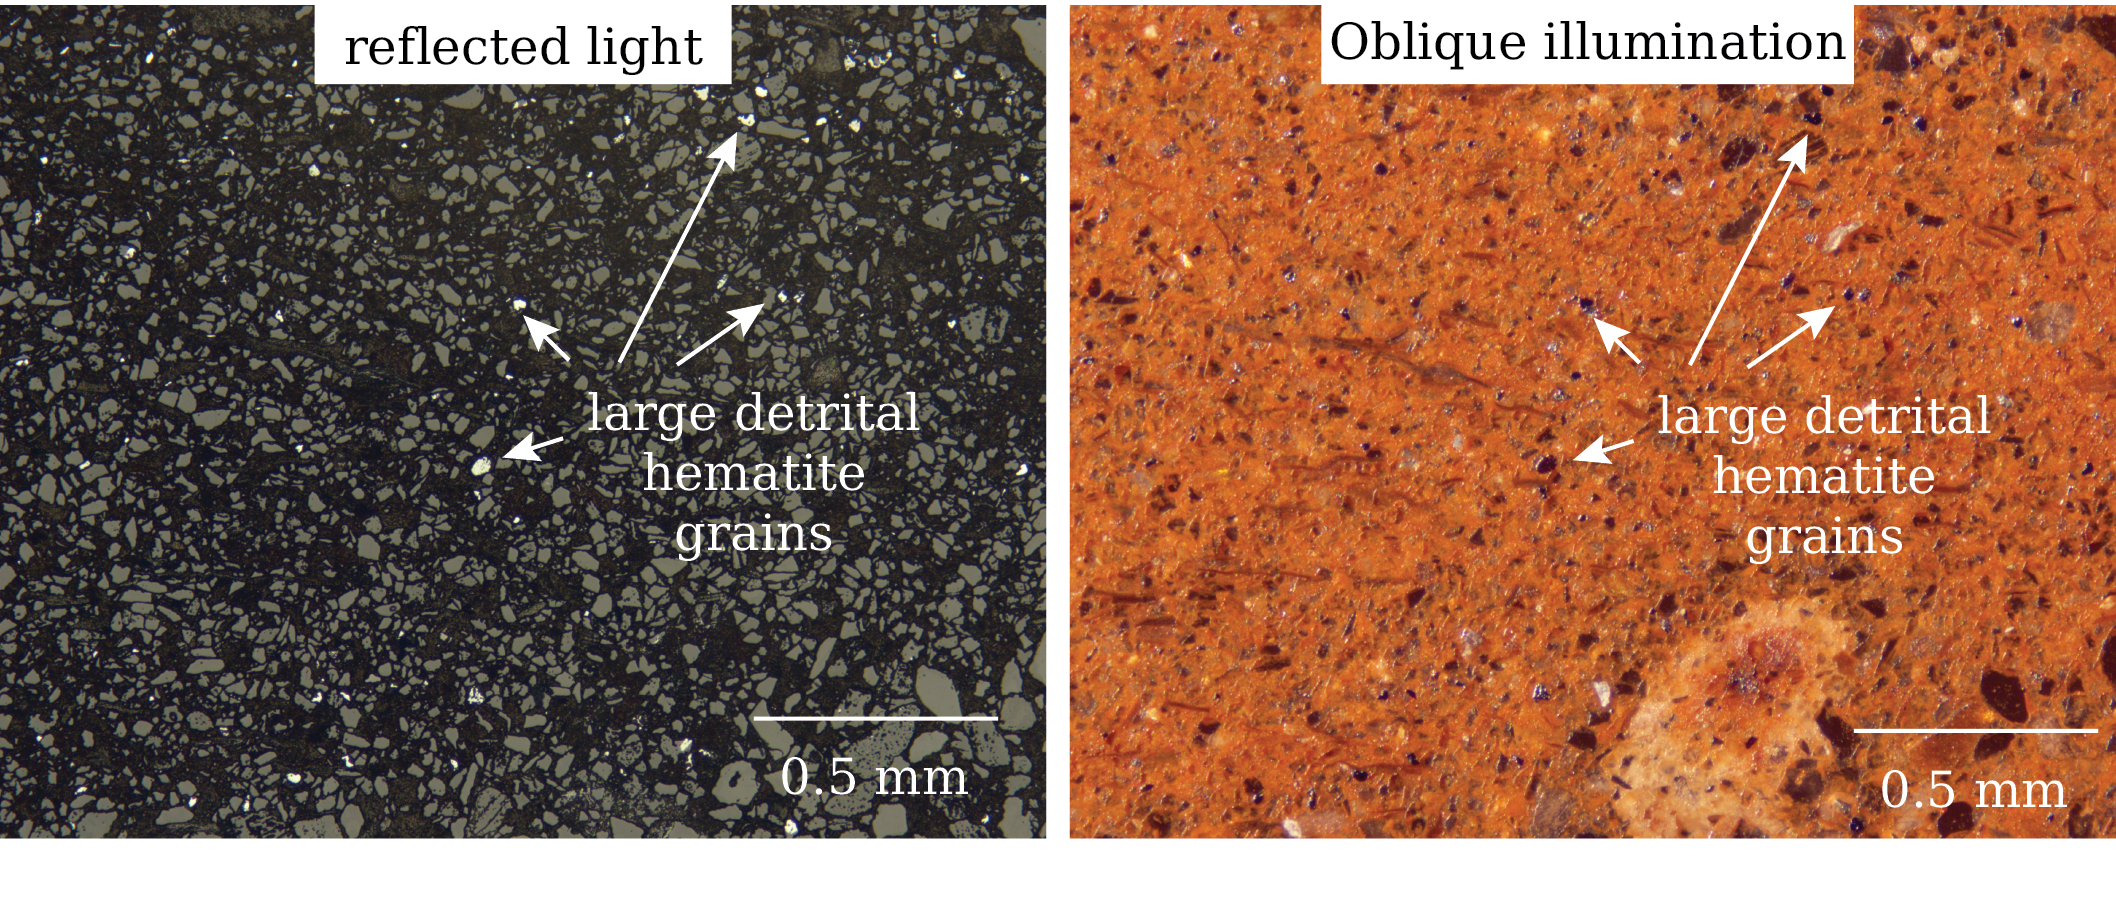
\includegraphics[width=0.9\textwidth]{figure/Zhang2024a/SI_petrography.png}
\caption{Side-by-side reflected light and oblique illumination images of a thin section of the same field of view of sample NW2-7 collected from Natural Wall ravine. The white arrows point towards examples of large sub-milimeter-scale detrital hematite grains that have bright reflectance under reflected light. Almost all subangular grains in grey color in the reflected image are quartz grains. The red color in the oblique illumination image is a result of diffuse reflectance of pigmentary hematite grains that often coat the boundaries of detrital grains. }
\label{fig:SI_petrography}
\end{figure}

\begin{figure}
\centering
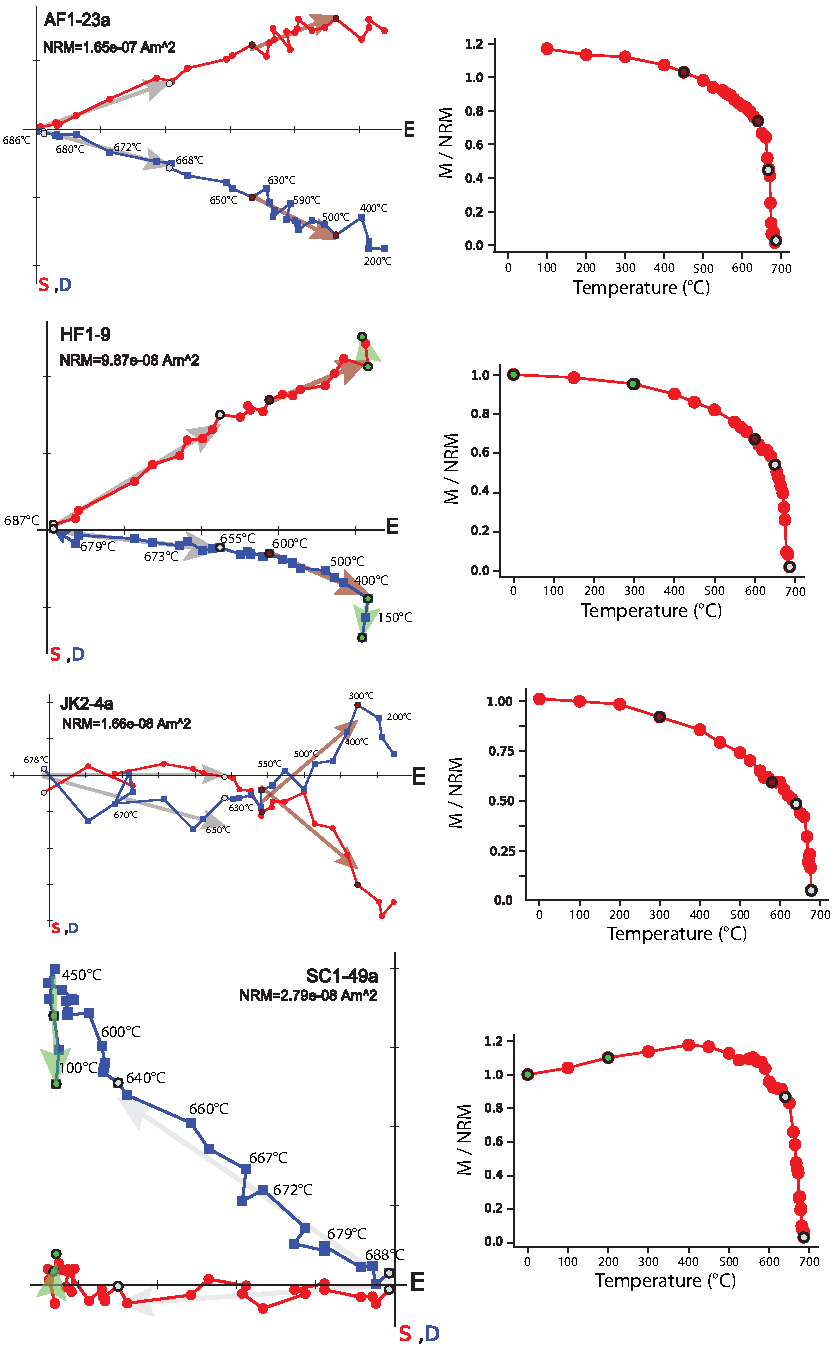
\includegraphics[width=0.6\textwidth]{figure/Zhang2024a/SI_orthogonal.pdf}
\caption{Representative orthogonal vector diagrams of demagnetization experiments for specimens from different stratigraphic sections of this study. An overprint component subparallel to the present day field direction in the study area is typically minimally present in siltstone to very fine-grained sandstone facies. This component shown in light green can be fit with a least-squares line in fine-grained facies. After the removal of the low-temperature component, a mid-temperature component typically unblocks through a wide range of temperature steps by up to $\sim$650\textdegree C. Finally, an origin-trending component with typically a shallower inclination than that of the mid-temperature component sharply unblocks through heating with smaller temperature intervals up toward the N\'eel temperature of hematite ($\sim$690\textdegree C). AF-Agate Falls section; HF-Hungarian side falls section near Dover Creek; JK-Hammel Creek section; SC-Snake Creek tributary section. M-magnetic moment; NRM-natural remanent magnetic moment. All diagrams are shown in tilt-corrected coordinates.}
\label{fig:SI_orthogonal}
\end{figure}

\begin{figure}
\centering
\includegraphics[width=0.5\textwidth]{figure/Zhang2024a/Jacobsville_pdf_directions.pdf}
\caption{Jacobsville present day local field directions. This present day overprint component is typically removed by $\sim$300\textdegree C.}
\label{fig:Jacobsville_pdf}
\end{figure}

\begin{figure}
\centering
\includegraphics[width=0.9\textwidth]{figure/Zhang2024a/SI_hct_fold_test.pdf}
\caption{Bootstrap paleomagnetic fold test \citep{Tauxe1994a} of the chemical remanent magnetization directions recorded by specimens from the nearly horizontal beds and moderately tilted beds at the Snake Creek tributary. Complete unfolding does not lie within the 95\% confidence limits of the test, consistent with the magnetization having been acquired syn- to post-folding.}
\label{fig:Jacobsville_hct_fold_test}
\end{figure}

\begin{figure}
\centering
\includegraphics[width=0.9\textwidth]{figure/Zhang2024a/SI_reversal_test.pdf}
\caption{Jacobsville detrital remanence directions showing dual polarities plotted on an equal area stereonet plot. The directions do not pass a reversal test of \cite{McFadden1990a} as the angle between the mean directions is 15.9\textdegree\, larger than the critical angle of 7.5\textdegree. The directions also do not pass the bootstrap reversal test of \cite{Tauxe1991a}. }
\label{fig:Jacobsville_reversal_test}
\end{figure}

\begin{figure}
\centering
\includegraphics[width=0.9\textwidth]{figure/Zhang2024a/SI_hct.pdf}
\caption{Jacobsville chemical remanence magnetization directions plotted by section. Samples collected from the Natural Wall section do not have interpretable chemical remanence component that can be fit with least-squares lines. All directions are plotted in geographic coordinates.}
\label{fig:Jacobsville_CRM}
\end{figure}

\begin{figure}
\centering
\includegraphics[width=0.75\textwidth]{figure/Zhang2024a/SI_Jacobsville_vs_Appalachian_poles.pdf}
\caption{Jacobsville detrital remanence Kent mean pole position and chemical remanence Fisher mean pole position (in geographic coordinates) plotted in context of Laurentia's paleomagnetic poles during Appalachian orogeny (ca. 460-260 Ma) as compiled in \cite{Torsvik2012a}. The mean chemical remanence pole position from the Snake Creek tributary section is plotted in context of the ca. 970-960 Ma poles developed by \cite{Brown2012a} from the Adirondack Highlands of the Grenville orogen. That this chemical remanence component failed a fold test (Figure S4) and yields a pole position that overlaps with the Grenville poles are consistent with the interpretation that the chemical remanence of the Jacobsville Formation at this locality was acquired  during the early Neoproterozoic, soon after Jacobsville deposition and deformation. That the Jacobsville DRM and CRM mean poles are distinct and far away from any of Laurentia's mid- to late-Paleozoic poles supports the interpretation that the Jacobsville detrital remanence magnetization was acquired during the Rigolet phase of the Grenvillian orogeny and the chemical remanence overprint was likely acquired soon after deposition as discussed in detail in the manuscript.}
\label{fig:Jacobsville_Appalachian}
\end{figure}

\begin{figure}
\centering
\includegraphics[width=0.9\textwidth]{figure/Zhang2024a/SI_Jacobsville_Nonesuch_rate.pdf}
\caption{Monte Carlo simulations of apparent polar wander rates implied by paleomagnetic and geochronologic data between the Nonesuch Formation and the Jacobsville Formation. (A) The gold and red points are 10,000 simulated Kent distribution mean paleomagnetic poles for the Nonesuch Formation and Jacobsville Formation, respectively. The simulated poles are connected by gray lines which represent the apparent polar wander great circle paths. (B) The points color-coded in the same way as in (A) show the simulated paleomagnetic pole latitudes plotted against their simulated pole ages using uniform distributions. The points are connected by gray lines which represent the simulated pole latitudinal motion. The histogram on the right shows all 10,000 of the simulated rates that yield the labeled 2.5 percentile value of 2.5 cm/yr, median value of 3.2 cm/yr and 97.5 percentile value of 4.3 cm/yr.}
\label{fig:Jacobsville_Nonesuch_rate}
\end{figure}

\begin{sidewaystable}
\tiny
\caption[Compilation of Laurentian paleomagnetic poles.]{\scriptsize Compilation of up-to-date Keweenawan Track paleomagnetic poles and ca. 780-720 Ma Laurentian paleomagnetic poles. }
\begin{tabular}{p{4cm}lllp{4cm}lllp{4cm}}

\hline
\multicolumn{9}{c}{Compilation of Fisher mean paleomagnetic poles}                                                                                                                                                                                        \\ \hline
Pole                                                       & Pole lat & Pole lon & A95  & Pole reference                                                         & AgeNominal & AgeLower & AgeUpper & Age reference                                       \\
Osler reverse (lower)                                      & 40.9     & 218.6    & 4.8  & \cite{Swanson-Hysell2014a}                                           & 1108       & 1105.15  & 1110     & \cite{Davis1985a, Swanson-Hysell2019a}               \\
Osler reverse (upper)                                      & 42.3     & 203.4    & 3.7  & \cite{Halls1974a, Davis1985a, Swanson-Hysell2014a} & 1105.15    & 1104.82  & 1105.48  & \cite{Swanson-Hysell2019a}                       \\
Mamainse lower reversed 1                                  & 49.5     & 227      & 5.3  & \cite{Swanson-Hysell2014b}                                           & 1109       & 1106     & 1112     & As discussed in \cite{Swanson-Hysell2019a}         \\
Mamainse lower reversed 2                                  & 37.5     & 205.2    & 4.5  & \cite{Swanson-Hysell2014b}                                                  & 1105       & 1100.4   & 1109     & \cite{Swanson-Hysell2014b}                              \\
Mamainse lower normal and upper reversed                   & 36.1     & 189.7    & 4.9  & \cite{Swanson-Hysell2014b}                                                  & 1100.36    & 1100.1   & 1100.61  & \cite{Swanson-Hysell2014b}                               \\
Mamainse upper normal                                      & 31.2     & 183.2    & 2.5  & \cite{Swanson-Hysell2014b}                                                  & 1094       & 1090     & 1100     & As discussed in S\cite{Swanson-Hysell2019a}            \\
Grand Portage Basalts                                      & 46       & 201.7    & 6.8  & \cite{Books1968a, Tauxe2009a}                                    & 1106       & 1105.28  & 1108     & \cite{Swanson-Hysell2019a}                         \\
North Shore Volcanic Group (upper NE   sequence)           & 31.1     & 181.7    & 4.2  & \cite{Books1972a, Tauxe2009a}                                    & 1095       & 1092     & 1098     & \cite{Davis1997a, Fairchild2017a}       \\
North Shore Volcanic Group (upper SW   sequence)           & 36.9     & 179.3    & 2.1  & \cite{Tauxe2009a, Swanson-Hysell2019a}                   & 1096.18    & 1093.94  & 1096.75  & \cite{Swanson-Hysell2019a}                        \\
Schroeder Lutsen Basalts                                   & 28.3     & 187.6    & 2.5  & \cite{Books1972a, Tauxe2009a, Fairchild2017a}            & 1090       & 1085     & 1091.5   & \cite{Fairchild2017a}                               \\
Portage Lake Volcanics                                     & 27.5     & 182.5    & 2.3  & \cite{Books1972a, Hnat2006a}                                         & 1092.51    & 1091.59  & 1093.37  & \cite{Swanson-Hysell2019a}                    \\
Lake Shore Traps                                           & 22.2     & 180.8    & 4.5  & \cite{Diehl1994a}                                                     & 1085.47    & 1084     & 1091     & \cite{Fairchild2017a, Swanson-Hysell2019a}    \\
Siemens Creek Volcanics                                    & 45.8     & 214      & 9.2  & \cite{Palmer1986a}                                                 & 1108       & 1105     & 1111     & \cite{Davis1997a}                               \\
Michipicoten Island Formation                              & 17       & 174.7    & 4.4  & \cite{Palmer1987a, Fairchild2017a}                        & 1083.95    & 1083.52  & 1084.39  & \cite{Fairchild2017a}                           \\
Freda Formation                                            & 2.2      & 179      & 4.2  & \cite{Henry1977a}                                                     & 1070       & 1060     & 1083.5   & As discussed in \cite{Swanson-Hysell2019a}            \\
Haliburton Intrusions                                      & -36.2    & 141.7    & 6.0  & \cite{Buchan1976a}                          & 1015       & 1000     & 1030     & \cite{Warnock2000a}                                          \\
Adirondack Highlands gneiss                                & -19      & 148.7    & 11.2 & \cite{Brown2012a}                                                &            &          &          &                                                     \\
Adirondack Highlands anorthositic rocks                    & -25.2    & 143.4    & 12.9 & \cite{Brown2012a}                                                &            &          &          &                                                     \\
Adirondack Highlands granites                              & -28.5    & 131.7    & 7.1  & \cite{Brown2012a}                                                &            &          &          &                                                     \\
Franklin large igneous province   Victoria/Mainland/Baffin & 6.7      & 162.1    & 3    & \cite{Denyszyn2009a}                                                   & 716.33     & 715.79   & 716.87   &                                                     \\
Combo Carbon Butte–Awatubi                                 & 14.2     & 163.8    & 3.5  & \cite{Eyster2019a}                                                   & 751        & 743.4    & 758.6    &                                                     \\
Carbon Canyon                                              & -0.5     & 166      & 9.7  & compilation by \cite{Eyster2019a}                                    & 757        & 750.2    & 763.8    &                                                     \\
UMG Group 3                                                & 4.9      & 160.6    & 3.2  & compilation by \cite{Eyster2019a}                                    & 755        &          &          & As discussed in \cite{Eyster2019a}                \\
Nankoweap                                                  & -10      & 163      & 4.9  & \cite{Weil2003a}                                                     & 782        &          &          & As discussed in Eyster et al., 2020                 \\
UMG Group 2                                                & -5.8     & 158.7    & 2.7  & compilation by \cite{Eyster2019a}                                    & 760        &          &          & As discussed in Eyster et al., 2021                 \\
UMG Group 1                                                & 3        & 163.5    & 3.2  & compilation by \cite{Eyster2019a}                                    & 766        &          &          & As discussed in Eyster et al., 2022                 \\
Gunbarrel mean                                             & 9.1      & 138.2    & 11.7 & \cite{Eyster2019a}                                                   & 774.93     & 774.39   & 775.47   &                                                    
\end{tabular}
\label{tab:pole_compilation}
\end{sidewaystable}

\clearpage

\begin{sidewaystable}
\begin{scriptsize}
\begin{tabular}{p{1.5cm}p{1cm}p{1cm}p{1cm}p{1cm}p{1cm}p{1cm}p{1cm}p{1cm}p{1cm}p{1cm}p{1cm}p{1cm}p{2cm}}
\hline
\multicolumn{14}{c}{Compilation of Kent mean paleomagnetic poles}                                                                                                                                                                                           \\ \hline 
Pole                  & Pole lat & Pole lon & Major axis lat & Major axis lon & Major axis magnitude & Minor axis lat & Minor axis lon & Minor axis magnitude & Pole reference         & Age Nominal & Age Lower & Age Upper & Age reference                                       \\
Nonesuch Formation    & 6.6      & 182.9    & 27.6           & 280.2          & 2.8                  & 41.6           & 87             & 2                    & \cite{Slotznick2023a} & 1080       & 1070     & 1083.5   & As discussed in \cite{Swanson-Hysell2019a}         \\
Jacobsville Formation & 16.9    & 183.4    & 45.2           & 255.5          & 4.1                    & 39.9           & 108.1          & 3.1                  & this study             & 990        & 985      & 992     & \cite{Hodgin2022a}; as discussed in the manuscript
\end{tabular}
\end{scriptsize}
\end{sidewaystable}

\clearpage



\chapter[Supporting Information for ``Paleomagnetism of the southwest Laurentia large igneous province and Cardenas Basalt: pulsed magmatism during rapid late Mesoproterozoic plate motion"][Supporting Information--SWLLIP]{Supporting Information for ``Paleomagnetism of the southwest Laurentia large igneous province and Cardenas Basalt: pulsed magmatism during rapid late Mesoproterozoic plate motion"}

\begin{figure}
\centering
\includegraphics[width=\textwidth]{figure/Zhang2024b/Cardenas_Unkar_geochem_major.pdf}
\caption[Major element geochemical data of the Cardenas Basalt and diabase intrusions in the Unkar Group.]{Total alkali-silica diagram of the Cardenas Basalt and mafic intrusions within the Unkar Group. The sills and dikes typically have lower silica content (basalt) than the Cardenas Basalt (basaltic trachy-andesite). Data for the Cardenas Basalt are from \cite{Hendricks1989a} and \cite{Larson1994a}. Data for the intrusions are from \cite{Hendricks1989a}.}
\label{fig:geochem_major}
\end{figure}

\begin{figure}
\noindent\includegraphics[width=5.8 in]{figure/Zhang2024b/SI_CB4.pdf}
\caption[Paleomagnetic data of Cardenas Basalt lava flow site CB4.]{\footnotesize Top panel: Thermal demagnetization data of paleomagnetic specimens collected near the bottom of lava flow CB4. Specimen CB4-2a has a demagnetization behavior similar to other lava flows--after the removal of the present day local field overprint, an origin-trending magnetite-carrying characteristic component unblocks up to 580\textdegree C. However, for all other specimens, after the removal of the present day local field overprint by $\sim$300\textdegree C (green vector), their total magnetic moments typically increase as the thermal demagnetization approaches $\sim$600\textdegree C. This mid-temperature component is followed by an origin-trending decay approaching the N\`eel temperature of hematite. Bottom panel: Bootstrap reversal test \citep{Tauxe1991a} of the mid-temperature and high-temperature remanence component of CB4. The directions pass the bootstrap reversal test and \cite{McFadden1990a} reversal test of  with a `C' classification. The high-temperature component that unblocks sharply near the hematite N\`eel temperature has the same polarity with titanomagnetite carried directions in other Cardenas Basalt flows. This similarity is consistent with the hematite forming from oxidation soon after eruption \citep{Haggerty1967a}. A likely origin of the antipodal component is that it is a self-reversed chemical remanent magnetization held by fine-grained hematite that formed as a result of inversion of maghemite precursors \citep{Hedley1968a, McClelland1987a, McClelland1993a, Swanson-Hysell2011a}. This self-reversal behavior is more likely than one that involves the reversal of the geomagnetic field after the emplacement of the CB4 lava flow. No reversed direction is observed in the adjacent lava flows and previous compilations of paleomagnetic data during this time suggest that the Cardenas lava flows were emplaced during a normal-polarity superchron \citep{Swanson-Hysell2019a, Driscoll2016b}.}
\label{fig:CB4_reversal_test}
\end{figure}

\begin{figure}
\noindent\includegraphics[width=5.8 in]{figure/Zhang2024b/SI_CBS1_CB11.pdf}
\caption[Paleomagnetic data of Cardenas Basalt lava flow site CB11 and the interflow sandstone site CBS1 below CB11.]{Top: Equal area plot showing the hematite magnetization specimen directions (orange) of the interflow sandstone CBS1 which is stratigraphically below the CB11 lava flow, whose magnetite magnetization directions are shown in purple. Bottom: Bootstrap common mean test of \cite{Tauxe1991a} between the specimens directions of the sandstone and the lava flow show a positive result. The specimen directions also passes a common mean test of \cite{McFadden1990a} with a `B' classification and have a positive support for sharing a common mean based on the Bayesian approach of \cite{Heslop2023a}.}
\label{fig:DV_tilt_test}
\end{figure}


\begin{figure}
\noindent\includegraphics[width=5.8 in]{figure/Zhang2024b/SI_tilt_test.pdf}
\caption[Death Valley diabase sill paleomagnetic tilt test]{Equal area plots showing the site-level directions and site-mean directions of the Death Valley diabase sills that yielded coherent within-site thermal demagnetization results in both geographic coordinates (left) and tilt-corrected coordinates (right). The site-mean direction in geographic coordinates is dec=295.1\textdegree, inc=8.9\textdegree, n=8, k=7.5, a$_{95}$=21.6\textdegree. The site-mean direction in tilt-corrected coordinates is dec=302.8\textdegree, inc=58.0\textdegree, k=34.8, a$_{95}$=9.5\textdegree. Applying tilt correction to the sills significantly improves the grouping of the site level directions. }
\label{fig:DV_tilt_test}
\end{figure}

\begin{figure}
\noindent\includegraphics[width=5.8 in]{figure/Zhang2024b/SI_Cardenas_QQ.png}
\caption[Cardenas Basalt VGPs Fisher distribution test]{Fisher quantile-quantile \cite{Fisher1987a} test of the distribution of the site level virtual geomagnetic poles of the Cardenas Basalt lava flows. The results show that the null hypothesis that the VGPs are Fisher-distributed cannot be rejected.}
\label{fig:Cardenas_QQ}
\end{figure}

\begin{figure}
\centering
\includegraphics[width=0.7\textwidth]{figure/Zhang2024b/Larson1994a_trace_elements.pdf}
\caption[Trace element geochemistry data of the Cardenas Basalt and the Hance sill.]{Trace element geochemistry data from \cite{Larson1994a}. The elemental abundance of the interior of the Hance sill is similar to that of the Cardenas Basalt lavas. Virtual geomagnetic poles developed from the Hance sill, Hance dike, and another undated sill in Red Canyon adjacent to Hance rapids plot closer to those of the Cardenas Basalt than the dated ca. 1098 Ma poles as shown in the main text. These data are consistent with the interpretation that the intrusions near Hance rapids are feeders to the Cardenas Basalt.}
\label{fig:trace_elements}
\end{figure}


\begin{sidewaystable}
\begin{footnotesize}
\caption[Compilation of paleomagnetic data developed from mafic sills in central Arizona by \cite{Harlan1993a} and \cite{Donadini2011a}.]{\scriptsize Compilation of paleomagnetic data collected from mafic sills in central Arizona by \cite{Harlan1993a} and \cite{Donadini2011a}. The study of \cite{Donadini2011a} revisited some field areas of \cite{Harlan1993a} and resampled some diabase sills in the earlier study. However, the determination of individual cooling units was not clear in \cite{Donadini2011a}. We compiled data from both studies with a focus on distinguishing individual paleomagnetic sites as distinct cooling units based on geographic and paleomagnetic information provided in the original publications. Data rejected by the original authors are not included. Original ``site" level data with better Fisher statistics (higher concentration parameter k values) are preferentially used in cases where repeat sampling of the same cooling unit is interpreted to have happened. We interpret site GD12 and GD13 of \cite{Harlan1993a} are the same as site OD in \cite{Donadini2011a} and thus recalculated mean statistics. dir\_dec---declination; dir\_inc--- inclination; k---kappa concentration parameter of the site mean direction; a$_{95}$---95\% confidence angle of site mean direction; n---number of samples included in each site; N---number of sites used in calculating the mean statistics by polarity; plat/Plat---pole latitude; plon/Plon---pole longitude. The site level pole locations are recalculating using the directions and site location information provided in the original studies.}
\begin{tabular}{p{3cm}p{1cm}p{1cm}p{1cm}p{1cm}p{1cm}p{1.2cm}p{1cm}p{3cm}p{1cm}p{1cm}p{1cm}}

site                   & dir\_dec & dir\_inc & k     & a95  & n  & slon    & slat  & pole reference                      & plon  & plat  & polarity \\
\hline 
GD01-02                & 279.2    & 57       &       &      &    & 249.5   & 33.7  & Harlan, 1993                        & 188.7 & 26.4  & N        \\
GD03                   & 285.3    & 51.4     & 165   & 3.6  & 11 & 249.5   & 33.8  & Harlan, 1993                        & 180.7 & 28.8  & N        \\
GD04                   & 295.5    & 56.6     & 81.9  & 7.7  & 7  & 249.5   & 33.8  & Harlan, 1993                        & 182.9 & 38.4  & N        \\
GD05                   & 283.2    & 26       & 108.5 & 5.8  & 7  & 249.5   & 33.8  & Harlan, 1993                        & 163.9 & 18.4  & N        \\
GD06-07                & 282.8    & 48.9     &       &      &    & 249.3   & 33.5  & Harlan, 1993                        & 179.3 & 25.8  & N        \\
GD08                   & 318      & 61.2     & 56.1  & 5.6  & 13 & 249.3   & 33.5  & Harlan, 1993                        & 186.8 & 56.1  & N        \\
GD09                   & 299.2    & 53.8     & 21.1  & 11.5 & 9  & 249.3   & 33.5  & Harlan, 1993                        & 178.3 & 40.3  & N        \\
GD10                   & 267.5    & 38.2     & 421.5 & 3.3  & 6  & 249.3   & 33.5  & Harlan, 1993                        & 178.7 & 9.7   & N        \\
GD17                   & 285.9    & 17.1     & 34.5  & 8.3  & 10 & 249.1   & 33.6  & Harlan, 1993                        & 157.7 & 18    & N        \\
GD18-20                & 339.6    & 36.3     &       &      &    & 249.2   & 33.5  & Harlan, 1993                        & 128   & 67.5  & N        \\
GD22                   & 270.1    & 40.4     & 120.3 & 5.1  & 8  & 249.5   & 33.8  & Harlan, 1993                        & 178.9 & 12.7  & N        \\
GD24                   & 297.9    & 58.5     & 168   & 4    & 9  & 249.5   & 33.8  & Harlan, 1993                        & 184.8 & 40.8  & N        \\
GD29                   & 306.9    & 66.4     & 678.5 & 2    & 9  & 249.4   & 33.6  & Harlan, 1993                        & 197.2 & 48.2  & N        \\
GD30                   & 264.1    & 33.4     & 157.6 & 5.4  & 6  & 249.4   & 33.6  & Harlan, 1993                        & 177.8 & 5.3   & N        \\
DF                     & 332.6    & 69.4     & 145.1 & 3.5  & 13 & 249.3   & 33.5  & Donadini et al., 2011               & 212.7 & 62.5  & N        \\
DG                     & 266.2    & 34.4     & 58.7  & 8    & 7  & 249.4   & 33.6  & Donadini et al., 2011               & 176.9 & 7.4   & N        \\
DJ                     & 281.9    & 52.8     & 325.5 & 2.9  & 9  & -110.48 & 33.65 & Donadini et al., 2011               & 182.8 & 26.7  & N        \\
KD                     & 293.8    & 13.4     & 142.3 & 3.3  & 14 & -110.97 & 33.89 & Donadini et al., 2011               & 151.2 & 23.5  & N        \\
MD                     & 277.2    & 50.7     & 110.4 & 4.2  & 12 & -110.98 & 33.87 & Donadini et al., 2011               & 182.9 & 22.2  & N        \\
GD12\_GD13\_OD         & 280.8    & 45.7     & 313.7 & 7    &    & -110.98 & 33.81 & Harlan, 1993; Donadini et al., 2011 & 177.6 & 23    & N        \\
GD11                   & 115.3    & -69.9    & 173.7 & 4.2  & 8  & -110.96 & 33.75 & Harlan, 1993                        & 24.3  & -41   & R        \\
GD15-27                & 224.9    & -73.7    &       &      &    & -110.5  & 33.8  & Harlan, 1993                        & 103.8 & -50.9 & R        \\
BD                     & 137.6    & -74      & 66.1  & 8.2  & 7  & -110.61 & 33.61 & Donadini et al., 2011               & 36.5  & -52   & R        \\
WD                     & 199.2    & -71      & 92.1  & 3.1  & 24 & -110.69 & 33.55 & Donadini et al., 2011               & 95    & -64.4 & R        \\
                       &          &          &       &      &    &         &       &                                     &       &       &          \\
\hline 
                       & dir\_dec & dir\_inc & k     & a95  & N  & Plon    & Plat  & A95                                 &       &       &          \\
\hline 
normal polarity mean   & 287.6    & 47.4     & 14.4  & 8.5  & 20 & 177.4   & 30.6  & 8.9                                 &       &       &          \\
reversed polarity mean & 167.4    & -77      & 31.8  & 16.6 & 4  & 239.9   & 57.5  & 30.6                                &       &       &         
\end{tabular}
\end{footnotesize}
\end{sidewaystable}

\clearpage







\end{document}